\documentclass[lang=en,mode = fancy,black]{elegantbook}
\usepackage[switch,mathlines]{lineno}
\usepackage{tikz-cd}
\usepackage{tikz}
\usepackage{bm}
\usepackage{amssymb}
\usepackage{cancel}
\usetikzlibrary{patterns}
\usepackage{braket}
\setcounter{tocdepth}{3}
\newcommand{\tr}{\mathrm{tr}}
\newcommand{\dd}{\mathrm{d}}
\newcommand{\bigzero}{\mbox{\normalfont\Large\bfseries 0}}
\newcommand{\rvline}{\hspace*{-\arraycolsep}\vline\hspace*{-\arraycolsep}}
\newcommand{\thermfrac}[3]{\left( \frac{\partial #1}{\partial #2} \right)_{#3}}
\newcommand{\jacobian}[4]{\frac{\partial \left(#1, #2\right)}{\partial \left(#3, #4\right)}}
\newcommand{\ppp}[2]{\frac{\partial #1}{\partial #2}}
\linenumbers
\title{量子力学笔记}
\author{梁莫言}
\institute{清华大学}
\date{\today}

\begin{document}
\frontmatter
\nolinenumbers

\begin{titlepage}
    \vspace{70cm}
    \begin{center}
        \begin{flushright}
        {\Large Notes on Quantum Mechanics} \\
        {\textit{Augustin--Ignace des Rameaux Leung Mouk--yin} }
        \vline
    \end{flushright}
    \vspace{20pt}
    \begin{figure*}[htbp!]
        \centering
        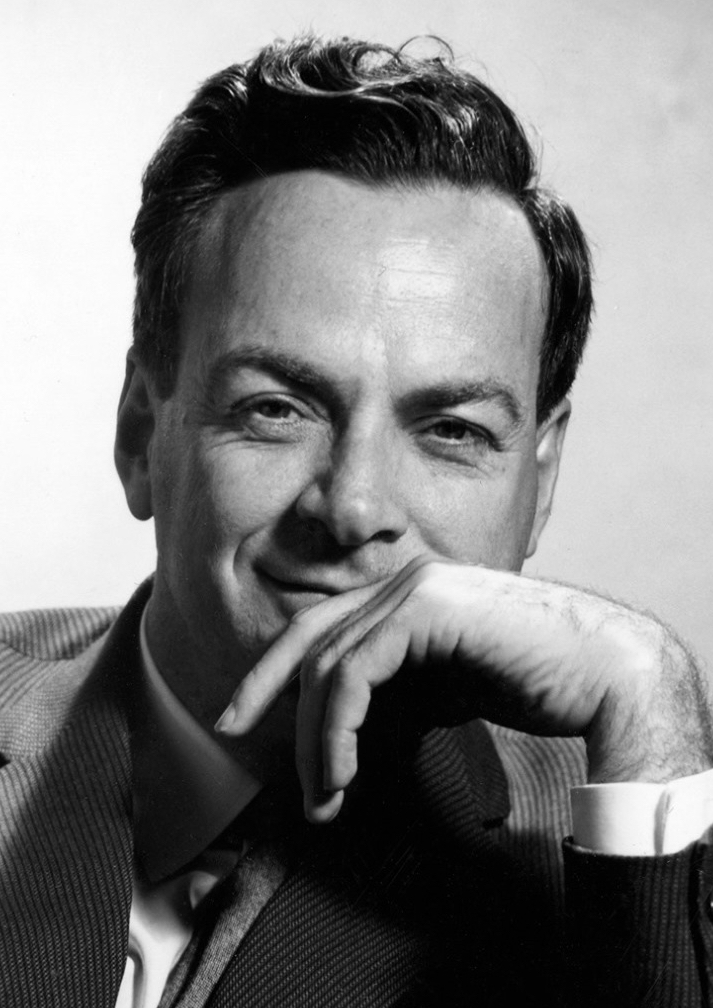
\includegraphics[scale=0.4]{graphics/Richard_Feynman_Nobel.jpg}\\
        {\large {Richard P. Feynman} }
    \end{figure*}
    \end{center}
    
    \newpage\pagestyle{empty}
    \topskip0pt
\vspace*{\fill}
\textsc{Ubi eras quando ponebam fundamenta terræ ; 
indica mihi, si habes intelligentiam.
Quis posuit mensuras ejus, si nosti ; 
vel quis tetendit super eam lineam ; Super quo bases illius solidatæ sunt ; 
aut quis demisit lapidem angularem ejus, cum me laudarent simul astra matutina,
et jubilarent omnes filii Dei ; Quis conclusit ostiis mare,
quando erumpebat quasi de vulva procedens;cum ponerem nubem vestimentum ejus,
et caligine illud quasi pannis infantiæ obvolverem ; 
Circumdedi illud terminis meis,
et posui vectem et ostia,
et dixi: Usque huc venies, et non procedes amplius,
et hic confringes tumentes fluctus tuos.
Numquid post ortum tuum præcepisti diluculo,
et ostendisti auroræ locum suum ; 
Et tenuisti concutiens extrema terræ,
et excussisti impios ex ea ; 
Restituetur ut lutum signaculum,
et stabit sicut vestimentum:
auferetur ab impiis lux sua,
et brachium excelsum confringetur.
Numquid ingressus es profunda maris,
et in novissimis abyssi deambulasti ; 
Numquid apertæ sunt tibi portæ mortis,
et ostia tenebrosa vidisti ; 
Numquid considerasti latitudinem terræ ; 
indica mihi, si nosti, omnia!}

\vspace*{\fill}
\end{titlepage}
\tableofcontents
\mainmatter
\linenumbers
\resetlinenumber
\include{chaps/history_modern_qm}
\include{chaps/hilbert_axiom}
\include{chaps/measurement_operators_spectra}
\chapter{Evolution Operators, Symmetries, and Conservation Laws}

\begin{note}
    This chapter is deductive in character. Taking the state-space axioms of Chapter~2 and the measurement axioms of Chapter~3 as established input, it adds exactly one new axiom --- the evolution postulate --- and derives its consequences: the Schr\"odinger equation as the postulate's theorem-form, the spectral resolution of the evolution operator, two exact two-state dynamics (spin precession and magnetic resonance), the time-ordered exponential for driven systems, symmetry transformations and Wigner's theorem, continuous symmetries treated as Lie groups, the Galilean group with its algebra derived and its central charge exhibited, the special status of time, conservation laws with good quantum numbers and selection rules, and the discrete symmetries of space and time. Two deep theorems (Stone's and Wigner's) are stated without proof and cited with pointers to the literature; everything provable with the machinery at hand is proved. It presupposes nothing beyond Chapters~2 and~3.
\end{note}

The preceding chapter closed with a question it had proved its own axioms cannot answer (Section~\ref{sec:ch3summary}):
\begin{quote}
    An observable is a self-adjoint operator, and a measurement is a projector's work. But the theory so far speaks only of interrogations: a preparation, then a question, then an answer. Between two measurements the counters are silent --- and the silence is an experimental fact with content, for interrogating identically prepared ensembles after different waiting times does not answer as ``nothing happened'' would predict: the next experiment's counts depend on the delay. Yet no axiom given so far contains the waiting time. What law governs the state between measurements? That is the theory of evolution, and it is the next chapter.
\end{quote}
This chapter is that theory.

The register of the answer differs from that of the first three chapters, and the difference is the book's, not merely the chapter's. Chapters~1--3 were inductive: from the crises of the old quantum theory and from the two-state experiments they distilled the state-space axioms (S1)--(S5) and the measurement axioms (M1)--(M5), admitting no formal object that had not first been earned on a bench. With those axioms in hand the book enters its second phase, in which the axioms are input and the theorems are output. Exactly one new axiom is added --- the evolution postulate of Section~\ref{sec:evolution-postulate} --- and everything else in the chapter is either proved from it and its predecessors, or cited honestly with the proof pointed to. Deduction does not mean detachment from the bench: by the charter of this phase, every section still lands on a measurable quantity --- precession and resonance frequencies, survival and beat laws, selection rules and degeneracies, and one phase between two orders of moving a system that no counter has yet exhibited.

The question is as old as the theory, and the shape of its answer was glimpsed at the theory's birth. Heisenberg's transition quantities of 1925 oscillated at the Bohr frequencies by construction, because the observed spectral lines demanded it (Section~\ref{subsec:matrix}); Schr\"odinger's wave equation of 1926, a controlled guess in Chapter~1's accounting, supplied a law of motion in one representation; and the distinction drawn there between kinematics and dynamics --- kinematics fixes what kind of object a state is and what questions may be asked of it, while dynamics says how the state evolves in time (Section~\ref{subsec:why-kinematics}) --- is exactly the border this chapter crosses. Wigner and Weyl brought the theory of group representations into quantum mechanics within a few years, preparing the modern understanding of symmetry that Chapter~1 deferred to a later chapter (Section~\ref{subsec:djv-formalism}). This is that chapter as well: the law of waiting and the theory of symmetry turn out to be one subject, because evolution is the model continuous family of transformations.

The route is deductive, but the landings are experimental. Section~\ref{sec:evolution-postulate} states the evolution postulate and proves its infinitesimal form; Section~\ref{sec:stationary-states} resolves the evolution operator into the spectrum of its generator and identifies what the eigenvalues physically are; Sections~\ref{sec:spin-precession} and~\ref{sec:time-ordered} solve the two-state dynamics exactly, first for a static field and then for a driven one, repaying the oldest two-state debt of the book, the Stern--Gerlach spin of Chapter~1. The chapter then turns to the transformations whose theory evolution completes: symmetry transformations, classified by Wigner's theorem (Section~\ref{sec:symmetry-transformations}); continuous symmetry families, recognized as Lie groups (Section~\ref{sec:lie-groups}); the Galilean group as the central worked example, with mass emerging as a central, superselected charge (Section~\ref{sec:galilean-group}); and the special status of time (Section~\ref{sec:time-status}). The harvest follows: conservation laws, good quantum numbers, degeneracy, and selection rules (Section~\ref{sec:conservation}); parity and time reversal (Section~\ref{sec:discrete-symmetries}); and at the exit, the ledger balanced and the next chapters' questions named (Section~\ref{sec:ch4summary}).

\section{Between Interrogations: the Evolution Postulate}
\label{sec:evolution-postulate}

The question is now posed with all its machinery in place. A system is prepared in the state $\ket{\psi(0)}$ at time $t = 0$; it is then left alone; at time $t$ it is interrogated. The counters of that interrogation depend on the delay --- that is the experimental content of the preceding chapter's exit question --- so the preparation and the delay together fix a state $\ket{\psi(t)}$, and waiting defines a map $\ket{\psi(0)} \mapsto \ket{\psi(t)}$. What can be said about that map a priori, before any particular system is studied? Four clauses, each a bench report with its operative constraint named, fix its form completely; and the form they fix is this chapter's single new axiom.

(i)~\emph{Linearity.} Between the preparation and the interrogation no record exists anywhere in the world of which alternative the system took --- that is what ``left alone'' means. By the marking clause of Chapter~2 (Section~\ref{sec:alternatives}), alternatives that leave no record combine by amplitudes, and amplitudes add: a superposition of preparations must evolve into the corresponding superposition of evolved states. The map of waiting is therefore a linear map on $\mathcal{H}$. The operative constraint is the absence of a record; where a record exists, the experiment is an interrogation and the law of this section does not apply to it.

(ii)~\emph{Unitarity.} At any delay, any complete question may be asked, and its outcome probabilities must sum to one: for every projection-valued measure, $\sum_n \braket{\psi(t)|P_n|\psi(t)} = \braket{\psi(t)|\psi(t)}$ by the Born rule \eqref{eq:pvm-born} and the resolution of identity \eqref{eq:resolution-identity}. The map of waiting therefore preserves the norm of every state. A linear map that preserves the norm of every vector preserves every inner product --- inner products are fixed linear combinations of norms, by the polarization identity \eqref{eq:polarization} --- and is therefore unitary \eqref{eq:unitary-def}. One loophole must be closed honestly, and it is closed inside the axiom itself. Probability sums alone would also permit an \emph{antilinear} norm-preserving map, of which complex conjugation in a fixed basis is the prototype. The composition law of clause (iv) below excludes the loophole: it gives $U(t) = U(t/2)\,U(t/2)$, so every member of the family is a square, and the square of \emph{either} norm-preserving kind is linear --- conjugating the scalars twice restores them. Hence every $U(t)$ is linear, hence unitary. The antilinear possibility is genuine physics, not a pedant's scruple: it returns exactly once in this book, where the reversal of motion forces it (Section~\ref{sec:discrete-symmetries}), and its classification theorem is Wigner's (Section~\ref{sec:symmetry-transformations}).

(iii)~\emph{Continuity.} The delayed counts vary continuously with the delay: no frequency has ever been observed to jump as a waiting time is dialed through any value. In the theory's language, $U(t)\ket{\psi}$ approaches $\ket{\psi}$ as $t \to 0$, for every prepared state --- strong continuity.

(iv)~\emph{Composition.} Waiting $s$ and then waiting $t$ is one way of waiting $s + t$, so $U(t+s) = U(t)\,U(s)$; and the law of waiting does not depend on when the preparation happened --- the homogeneity of time --- so one and the same family $U(t)$ serves at every epoch, with $U(0) = I$. It is this clause that makes the family a \emph{one-parameter group}: composition is addition of the parameter. The vocabulary is Section~\ref{sec:lie-groups}'s; the fact is the bench's.

None of these clauses is a theorem, and this section does not pretend otherwise: each is a plausibility argument whose operative constraint has been named, and together they fix the form of the law. That form we now postulate.

\medskip\noindent\textbf{Axiom D1 (evolution between interrogations).} \emph{Between a preparation and the next interrogation, the state of an isolated system is carried by a family of linear operators $U(t)$, one for each waiting time:}
\begin{linenomath}
    \begin{equation}
        \ket{\psi(t)} = U(t)\,\ket{\psi(0)}, \qquad U(t+s) = U(t)\,U(s), \qquad U(0) = I, \qquad U(t)^\dagger\,U(t) = I,
        \label{eq:evolution-axiom}
    \end{equation}
\end{linenomath}
\emph{with the family strongly continuous in $t$.}

The axiom's whole content is infinitesimal: a family obeying the composition law is determined by its behavior at $t = 0$, and the object sitting there is the theory's first generator. In finite dimension the statement is elementary. A continuous unitary family is differentiable; differentiating $U(t)^\dagger U(t) = I$ at $t = 0$ gives $U'(0)^\dagger = -U'(0)$, so the operator $i\hbar\,U'(0)$ equals its adjoint. In the general case the differentiability itself is deep, and its theorem is cited, not proved.

\medskip\noindent\textbf{Theorem (Stone, stated without proof).} \emph{Every strongly continuous one-parameter unitary family \eqref{eq:evolution-axiom} has a unique self-adjoint generator $H$:}
\begin{linenomath}
    \begin{equation}
        U(t) = e^{-iHt/\hbar}, \qquad H := i\hbar\left.\frac{\dd U}{\dd t}\right|_{t=0},
        \label{eq:generator-def}
    \end{equation}
\end{linenomath}
\emph{where the exponential is the function $e^{-ixt/\hbar}$ of the observable $H$ in the sense of Chapter~3's function-of-an-observable rule \eqref{eq:function-of-observable}.}\footnote{M.~H. Stone, \emph{Ann. of Math.}~\textbf{33}, 643 (1932). For unbounded $H$ the exponential is defined through the spectral resolution, and the domain questions it raises belong to Appendix~A; the spectral reading of the display is made explicit in Section~\ref{sec:stationary-states}.} The insertion of $\hbar$ is, at this stage, dimensional only: $U'(0)$ is a rate, with units of inverse time, and multiplication by the quantum of action gives the generator the \emph{units} of energy. Whether the generator \emph{is} the energy observable is a physical question, not settled by a choice of units; it is earned in Section~\ref{sec:stationary-states}.

\medskip\noindent\textbf{Theorem (Schr\"odinger equation; the theorem-form of D1).} \emph{Every state evolving by \textup{(D1)} obeys}
\begin{linenomath}
    \begin{equation}
        i\hbar\,\frac{\dd}{\dd t}\ket{\psi(t)} = H\,\ket{\psi(t)},
        \label{eq:schroedinger}
    \end{equation}
\end{linenomath}
\emph{with $H$ the generator \eqref{eq:generator-def}.} The proof is one line of calculus on the family law:
\begin{linenomath}
    \begin{equation*}
        \frac{\dd U}{\dd t}\bigg|_{t} = \lim_{\varepsilon\to 0}\frac{U(t+\varepsilon) - U(t)}{\varepsilon} = \lim_{\varepsilon\to 0}\frac{U(\varepsilon) - I}{\varepsilon}\,U(t) = U'(0)\,U(t) = -\frac{i}{\hbar}\,H\,U(t),
    \end{equation*}
\end{linenomath}
and applying both sides to $\ket{\psi(0)}$ gives \eqref{eq:schroedinger}. The equation is therefore honestly labeled: it is not a new axiom but the infinitesimal register of (D1), and the two say one thing. In finite dimension the loop closes elementarily, without Stone's theorem: the equation $i\hbar\,\dd U/\dd t = HU$ with $U(0) = I$ has the unique solution $U(t) = e^{-iHt/\hbar}$, as differentiation of the exponential series shows at once. The generator $H$ is called the \textbf{Hamiltonian} of the system. The name is so far only a name; its physical reading as the energy is earned by the Bohr-frequency identification of Section~\ref{sec:stationary-states} and sealed by the time-translation analysis of Sections~\ref{sec:galilean-group} and~\ref{sec:time-status}.

The equation has stood in this book twice before, and both appearances are now discharged. Chapter~1 recorded Schr\"odinger's wave equation of 1926 as a controlled guess, and its equivalence section recorded the component law $i\hbar\,\dot c_m = \sum_n H_{mn} c_n$ of matrix mechanics (Section~\ref{subsec:equivalence}). What \eqref{eq:schroedinger} adds is deductive status: the law of motion is proved from (D1), abstract and representation-free --- no longer a guess, and no longer tied to any representation. Its wave-mechanical specialization remains the next chapter's.

One operational remark belongs to this section, stated once and not developed. Throughout this chapter, $t$ is the experimenter's waiting time, read from the laboratory clock: a parameter of the description, not an observable of the system --- no counter registers it. The structural consequences of that status (there is no time operator, and the Hamiltonian's role is dual) are analyzed in Section~\ref{sec:time-status}.

\begin{note}
Two laws, two jurisdictions. Between a preparation and the next interrogation, the state obeys (D1) alone: the evolution is continuous, deterministic, and reversible. At an interrogation, the measurement axioms (M1)--(M5) take over: the outcomes are random with Born-rule frequencies, and the conditional state is the L\"uders update \eqref{eq:luders-update} --- discontinuous and irreversible. The joint protocol of the theory is: evolve by \eqref{eq:schroedinger} between interrogations; update by \eqref{eq:luders-update} at one. Which physical event constitutes an interrogation --- when nature applies the second clause rather than the first --- the formalism does not say; that is the measurement problem, and it belongs to the chapter on composite systems.
\end{note}

The theorem's first consequence is a survival law, and it is measurable. Ask the simplest delayed question of all: is the system still in the state in which it was prepared? The survival amplitude is expanded from the exponential series of \eqref{eq:generator-def}:
\begin{linenomath}
    \begin{equation*}
        \begin{aligned}
            \braket{\psi(0)|\psi(t)}
            &= \braket{\psi(0)|e^{-iHt/\hbar}|\psi(0)}
             = \braket{\psi(0)|\Bigl(I - \frac{i}{\hbar}Ht - \frac{1}{2\hbar^2}H^2t^2 + O(t^3)\Bigr)|\psi(0)} \\[4pt]
            &= 1 - \frac{i}{\hbar}\langle H\rangle_\psi\,t - \frac{1}{2\hbar^2}\langle H^2\rangle_\psi\,t^2 + O(t^3) .
        \end{aligned}
    \end{equation*}
\end{linenomath}
For the squared modulus, set $a := \frac{t}{\hbar}\langle H\rangle_\psi$ and $b := \frac{t^2}{2\hbar^2}\langle H^2\rangle_\psi$, so that $\braket{\psi(0)|\psi(t)} = 1 - ia - b + O(t^3)$. Then
\begin{linenomath}
    \begin{equation*}
        \begin{aligned}
            P(t) := \bigl|\braket{\psi(0)|\psi(t)}\bigr|^2
            &= |1 - ia - b|^2 + O(t^4)
             = (1 - b)^2 + a^2 + O(t^4) \\
            &= 1 - 2b + a^2 + O(t^4)
             = 1 - \frac{t^2}{\hbar^2}\langle H^2\rangle_\psi + \frac{t^2}{\hbar^2}\langle H\rangle_\psi^2 + O(t^4)
             = 1 - \frac{t^2}{\hbar^2}\bigl(\langle H^2\rangle_\psi - \langle H\rangle_\psi^2\bigr) + O(t^4) .
        \end{aligned}
    \end{equation*}
\end{linenomath}
Collecting the variance via \eqref{eq:variance}:
\begin{linenomath}
    \begin{equation}
        \braket{\psi(0)|\psi(t)} = 1 - \frac{i}{\hbar}\langle H\rangle_\psi\,t - \frac{t^2}{2\hbar^2}\langle H^2\rangle_\psi + O(t^3), \qquad P(t) = 1 - \frac{(\Delta H)^2}{\hbar^2}\,t^2 + O(t^4),
        \label{eq:quadratic-survival}
    \end{equation}
\end{linenomath}
with $(\Delta H)^2 := \langle H^2\rangle_\psi - \langle H\rangle_\psi^2$ the generator's variance \eqref{eq:variance} in the prepared state. Two readings of the display are experimental. First, no survival curve ever begins linearly: every decay starts flat, with a curvature set by the spread of the preparation over the generator's eigenvalues. Second, the flatness is exploitable: re-interrogating the survival question $n$ times at intervals $t/n$ returns the survival probability $P(t/n)^n \simeq \bigl(1 - (\Delta H)^2 t^2/\hbar^2 n^2\bigr)^n \longrightarrow 1$ as $n \to \infty$ --- watched sufficiently often, the state ceases to change. This is the \emph{quantum Zeno effect}, named once and not developed further.\footnote{B.~Misra and E.~C.~G.~Sudarshan, \emph{J. Math. Phys.}~\textbf{18}, 756 (1977).}

The advantage of (D1) is its economy: a single axiom carries the entire dynamics of the theory, and every clause of it is a bench report --- linearity from the absence of records between interrogations, unitarity from the freedom to ask any complete question at any delay, continuity from the smooth drift of the counts, composition from the homogeneity of time. Its limitation is equally sharp: the postulate says \emph{that} a self-adjoint generator exists, never \emph{which} generator a given system has. The Hamiltonian is physical input, identified case by case; the two-state instances of Sections~\ref{sec:spin-precession} and~\ref{sec:time-ordered} are phenomenological identifications, measured rather than derived, and Section~\ref{sec:galilean-group} will show how far symmetry alone can carry the generator of a free system.

The generator is in hand, but its eigenvalues are so far anonymous numbers: the theorem provides the operator, not their physical reading. What those eigenvalues \emph{are} --- and how the whole evolution decomposes into them --- is the spectral resolution of $U(t)$, the subject of the next section.

\section{Stationary States and the Spectral Resolution of $U(t)$}
\label{sec:stationary-states}

The evolution postulate hands us a self-adjoint generator, and Chapter~3 hands us the language to read it: by the spectral theorem \eqref{eq:eigenproblem}, $H$ resolves into eigenvalues and projectors, $H = \sum_n E_n\,P_n$ \eqref{eq:spectral-decomposition}, with the degenerate form \eqref{eq:spectral-degenerate} when levels repeat. This section solves the evolution postulate in that language --- and in the solution discovers what the eigenvalues physically are.

The exponential of \eqref{eq:generator-def} is the function $e^{-ixt/\hbar}$ of the observable $H$, in the sense of Chapter~3's function-of-an-observable rule \eqref{eq:function-of-observable}:
\begin{linenomath}
    \begin{equation}
        U(t) = e^{-iHt/\hbar} := \sum_n e^{-iE_n t/\hbar}\,P_n .
        \label{eq:evolution-operator}
    \end{equation}
\end{linenomath}
That this family satisfies every clause of (D1) is a computation with the projector algebra \eqref{eq:projector-algebra}: orthogonality $P_m P_n = 0$ ($m \neq n$) collapses the double sum in $U(t)U(s)$ to $\sum_n e^{-iE_n(t+s)/\hbar}P_n = U(t+s)$; idempotence and the resolution of identity \eqref{eq:resolution-identity} give $U(0) = \sum_n P_n = I$; and the reality of the $E_n$ gives $U(t)^\dagger U(t) = \sum_n P_n = I$. Term-by-term differentiation gives $i\hbar\,\dd U/\dd t = \sum_n E_n e^{-iE_n t/\hbar}P_n = H\,U(t)$, the Schr\"odinger equation \eqref{eq:schroedinger}. In finite dimension nothing further is needed; the convergence questions of the infinite case are Appendix~A's.\footnote{For an unbounded $H$ the sum is replaced by an integral over the spectrum, and the differentiability statements hold on the generator's domain; see Appendix~A.}

An eigenray of the generator evolves by a phase and nothing more, and a general preparation decomposes into such eigenrays:
\begin{linenomath}
    \begin{equation}
        \ket{e_n(t)} = e^{-iE_n t/\hbar}\ket{e_n}, \qquad \ket{\psi(t)} = \sum_n c_n\,e^{-iE_n t/\hbar}\ket{e_n}, \qquad c_n = \braket{e_n|\psi(0)} .
        \label{eq:stationary-phase}
    \end{equation}
\end{linenomath}
By the ray theorem (Section~\ref{sec:rays}), a state changed only by a phase is the same state: a preparation sharp in the generator is physically unchanged by waiting, and every interrogation answers at time $t$ exactly as it answered at time $0$. Such eigenrays are called \emph{stationary states}. (They are eigenrays of $H$; no wave functions are involved or needed.) All the time dependence of a general state lives in the \emph{relative} phases $e^{-i(E_m - E_n)t/\hbar}$ of its stationary components.

Insert the expansion into the expectation of any fixed operator $A$:
\begin{linenomath}
    \begin{equation}
        \langle A\rangle(t) = \braket{\psi(t)|A|\psi(t)} = \sum_{m,n} c_m^{*}c_n\,e^{i(E_m - E_n)t/\hbar}\,\braket{e_m|A|e_n} .
        \label{eq:bohr-frequencies}
    \end{equation}
\end{linenomath}
Every time dependence of every expectation value is a sum of oscillations at the frequencies $\omega_{mn} := (E_m - E_n)/\hbar$ --- the \emph{Bohr frequencies} of the generator. This is exactly the time dependence Heisenberg imposed on his transition quantities in 1925, because the observed spectral lines come at such differences (Section~\ref{subsec:matrix}); here it is not imposed but derived, the dynamical repayment of that debt. And the empirical warrant Heisenberg had --- the combination principle, that spectral lines are differences of terms (Section~\ref{subsec:matrix}) --- is now turned into an identification, stated with its register made plain: \textbf{the eigenvalues of the generator are the energy levels of the system, and the generator $H$ is the energy observable.} The identification is physical, not definitional; its structural sealing --- time translation exhibited as the evolution family's place among the spacetime symmetries --- is the work of Sections~\ref{sec:galilean-group} and~\ref{sec:time-status}. Stationary states are now named honestly: they are the energy-sharp preparations.

One clause of \eqref{eq:bohr-frequencies} deserves isolating at once: an operator with no matrix elements between distinct eigenrays, $\braket{e_m|A|e_n} = 0$ for $m \neq n$, has a constant expectation in every state. Which operators these are, and why, is the conservation theorem of Section~\ref{sec:conservation}.

The two-state case computes the display end to end, and it is the book's first exact dynamics. The general two-state generator is Chapter~3's \eqref{eq:hermitian-2d}: $H = a_0\,I + \bm a\cdot\bm\sigma$, with eigenvalues $E_\pm = a_0 \pm |\bm a|$ and eigenrays the spin alternatives along $\pm\hat{\bm a}$. Take $\hat{\bm a} = \hat{\bm z}$ and prepare the state $\ket{+x} = (\ket{+z} + \ket{-z})/\sqrt{2}$ of Chapter~1's two-state grammar (Section~\ref{sec:twostate}). The state decomposes into the two stationary rays,
\begin{linenomath}
    \begin{equation*}
        \ket{\psi(t)} = \frac{1}{\sqrt{2}}\Bigl(e^{-i(a_0+|\bm a|)t/\hbar}\ket{+z} + e^{-i(a_0-|\bm a|)t/\hbar}\ket{-z}\Bigr),
    \end{equation*}
\end{linenomath}
and every expectation with off-diagonal content oscillates at the single Bohr frequency $\omega = (E_+ - E_-)/\hbar = 2|\bm a|/\hbar$:
\begin{linenomath}
    \begin{equation*}
        \langle\sigma_x\rangle(t)
        = \braket{\psi(t)|\sigma_x|\psi(t)}
        = \frac{1}{2}\Bigl(e^{i\omega t}\braket{+z|\sigma_x|-z} + e^{-i\omega t}\braket{-z|\sigma_x|+z}\Bigr)
        = \frac{1}{2}\bigl(e^{i\omega t} + e^{-i\omega t}\bigr)
        = \cos\omega t,
    \end{equation*}
\end{linenomath}
using $\sigma_x\ket{\pm z} = \ket{\mp z}$ from the Pauli algebra of Chapter~3 \eqref{eq:sigma-commutator}; a complete oscillation of the ensemble's answer between the $+x$ and $-x$ alternatives. Two measurables of this kind carry names. The intensity modulation of a radiating ensemble whose atoms are coherently excited into a superposition of two nearby levels is the \emph{quantum beat}, read off at the Bohr frequency of the pair. And Ramsey's separated-field method --- two short interrogations bracketing a free wait --- reads the accumulated relative phase directly, the working principle of atomic frequency standards. The overall rate $a_0/\hbar$ appears in no count: a common phase is unobservable (Section~\ref{sec:rays}), and only eigenvalue \emph{differences} are measured --- the combination principle again, now a theorem-clause of the evolution law.

The beat was abstract: $a_0$ and $\bm a$ were numbers without an apparatus. The oldest two-state system of this book --- the spin of the Stern--Gerlach benches --- realizes it literally when a magnetic field does the driving. That realization, solved exactly, is next.

\section{Spin in a Magnetic Field: Precession Solved Exactly}
\label{sec:spin-precession}

The Stern--Gerlach benches of Chapter~1 (Section~\ref{sec:twostate}, Figure~\ref{fig:stern_gerlach}) gave this book its first two-state system, and Pauli's two-valuedness gave the electron its spin (Section~\ref{subsec:spin}). The debt recorded then comes due now in its dynamical share: what does a spin \emph{do} between interrogations? In a static magnetic field the answer is exact, and it is this chapter's flagship computation.

A spin carries a magnetic moment $\bm\mu = \gamma\,\bm S$, with $\bm S = (\hbar/2)\,\bm\sigma$ the spin operator of Chapter~3 \eqref{eq:sigma-n-def} and $\gamma$ the particle's gyromagnetic ratio --- a measured constant of the particle, known from the Stern--Gerlach deflection itself and read with precision by the resonance of Section~\ref{sec:time-ordered}. The coupling to a field $\bm B = B\bm n$ is $H = -\bm\mu\cdot\bm B$:
\begin{linenomath}
    \begin{equation*}
        H = -\gamma\,\bm B\cdot\bm S = -\frac{\gamma\hbar B}{2}\,(\bm n\cdot\bm\sigma) =: \frac{\hbar\omega}{2}\,(\bm n\cdot\bm\sigma), \qquad \omega := -\gamma B .
    \end{equation*}
\end{linenomath}
The identification is phenomenological in the sense of Section~\ref{sec:evolution-postulate}'s limitation: the form of the generator is measured, not derived. The Larmor frequency $\omega$ carries the sign of $-\gamma$ (the electron's $\gamma$ is negative, its $\omega$ positive); the sign fixes only the sense of the precession, and $|\omega|$ is what the bench measures.

The evolution operator follows in closed form. The Pauli algebra recorded with \eqref{eq:hermitian-2d} gives $(\bm n\cdot\bm\sigma)^2 = I$, so the exponential series splits into its even and odd powers, the two subseries being those of the cosine and the sine:
\begin{linenomath}
    \begin{equation}
        U(t) = e^{-i\omega t\,(\bm n\cdot\bm\sigma)/2} = \cos\frac{\omega t}{2}\,I - i\,\sin\frac{\omega t}{2}\,(\bm n\cdot\bm\sigma) .
        \label{eq:larmor-evolution}
    \end{equation}
\end{linenomath}

Choose the field along $z$ and expand the state as $a\ket{+z} + b\ket{-z}$, with $a,b$ the complex coefficients at $t=0$. By \eqref{eq:larmor-evolution} with $\bm n = \hat{\bm z}$,
\begin{linenomath}
    \begin{equation*}
        U(t) = \cos\frac{\omega t}{2}\,I - i\,\sin\frac{\omega t}{2}\,\sigma_z
        = \begin{pmatrix}
            e^{-i\omega t/2} & 0 \\[2pt] 0 & e^{+i\omega t/2}
        \end{pmatrix},
    \end{equation*}
\end{linenomath}
so the two components evolve as $a(t) = a\,e^{-i\omega t/2}$ and $b(t) = b\,e^{+i\omega t/2}$. Now form the combination that extracts the off-diagonal content:
\begin{linenomath}
    \begin{equation*}
        \langle\sigma_x\rangle(t) + i\langle\sigma_y\rangle(t)
        = \braket{\psi(t)|(\sigma_x + i\sigma_y)|\psi(t)}
        = \begin{pmatrix} a(t)^{*} & b(t)^{*} \end{pmatrix}
          \begin{pmatrix} 0 & 2 \\ 0 & 0 \end{pmatrix}
          \begin{pmatrix} a(t) \\ b(t) \end{pmatrix}
        = 2\,a(t)^{*}b(t) .
    \end{equation*}
\end{linenomath}
Inserting the evolved coefficients,
\begin{linenomath}
    \begin{equation*}
        \langle\sigma_x\rangle(t) + i\langle\sigma_y\rangle(t)
        = 2\,(a^{*}e^{+i\omega t/2})(b\,e^{+i\omega t/2})
        = 2a^{*}b\,e^{+i\omega t}
        = \bigl(\langle\sigma_x\rangle(0) + i\langle\sigma_y\rangle(0)\bigr)\,e^{+i\omega t},
    \end{equation*}
\end{linenomath}
and the conjugate combination gives the minus sign. Meanwhile $\langle\sigma_z\rangle(t) = |a(t)|^{2} - |b(t)|^{2} = |a|^{2} - |b|^{2} = \langle\sigma_z\rangle(0)$, since the phases cancel in each squared modulus. For the $+x$ recapture, with $\ket{\psi(0)} = \ket{+x} = (\ket{+z}+\ket{-z})/\sqrt{2}$ we have $a=b=1/\sqrt{2}$, so $a(t) = e^{-i\omega t/2}/\sqrt{2}$, $b(t) = e^{+i\omega t/2}/\sqrt{2}$, and
\begin{linenomath}
    \begin{equation*}
        P_{+x\to+x}(t) = \bigl|\braket{+x|\psi(t)}\bigr|^{2}
        = \Bigl|\frac{1}{\sqrt{2}}\bigl(a(t)+b(t)\bigr)\Bigr|^{2}
        = \frac{1}{4}\,\bigl|e^{-i\omega t/2}+e^{+i\omega t/2}\bigr|^{2}
        = \cos^{2}\frac{\omega t}{2} .
    \end{equation*}
\end{linenomath}
Collecting the results:
\begin{linenomath}
    \begin{equation}
        \langle\sigma_x\rangle(t) \pm i\,\langle\sigma_y\rangle(t) = e^{\pm i\omega t}\bigl(\langle\sigma_x\rangle(0) \pm i\,\langle\sigma_y\rangle(0)\bigr), \qquad \langle\sigma_z\rangle(t) = \langle\sigma_z\rangle(0); \qquad P_{+x\,\to\,+x}(t) = \cos^2\frac{\omega t}{2} .
        \label{eq:precession}
    \end{equation}
\end{linenomath}
The expectation vector rotates about the field axis at the rate $\omega$ with its $z$-component frozen --- Larmor precession. The third clause is the exit question of Chapter~3 (Section~\ref{sec:ch3summary}) turned into a number: a $\ket{+x}$ beam, left to wait in the field and then re-interrogated along $x$, answers $+x$ with a frequency $\cos^2(\omega t/2)$ that oscillates between one and zero, although nothing was recorded in between.

\begin{note}
The motion of the expectation vector has an evident geometric reading: the arrow $(\langle\sigma_x\rangle, \langle\sigma_y\rangle, \langle\sigma_z\rangle)$ rotates about the field axis. The reading is correct, but this section has used no rotation theory: every display above is $2\times 2$ matrix arithmetic. The identification of that arithmetic with the geometry of rotations is a theorem of Sections~\ref{sec:lie-groups} and~\ref{sec:galilean-group}, not an assumption of this one.
\end{note}

One full period of the precession returns the state with a sign:
\begin{linenomath}
    \begin{equation}
        U(2\pi/\omega) = \cos\pi\,I - i\,\sin\pi\,(\bm n\cdot\bm\sigma) = -I .
        \label{eq:spinor-sign}
    \end{equation}
\end{linenomath}
By the ray theorem (Section~\ref{sec:rays}) the sign changes no count: after a full Larmor period every interrogation answers as it did before. Yet the $-1$ is not nothing. It is exactly the sign Chapter~2 recorded as an experimental fact of neutron interferometry (Section~\ref{sec:rays}): a rotation through $4\pi$, not $2\pi$, is required to return a spin-$\tfrac12$ state to itself. And the precession operator $e^{-i\theta\,(\bm n\cdot\bm\sigma)/2}$ has precisely the form of a rotation representative acting on the two-state system --- angle $\theta$ about the axis $\bm n$, with the characteristic half-angle. That Larmor precession \emph{is} a rotation of the spin state is named here; it is earned where the rotation generators are derived (Section~\ref{sec:galilean-group}), and its full interpretation remains the angular-momentum chapter's declared debt.

The measurable landing of the computation is the precession frequency itself. Magnetic resonance --- Rabi's molecular-beam method\footnote{I.~I.~Rabi, \emph{Phys. Rev.}~\textbf{51}, 652 (1937). The method's exact theory is the driven problem of Section~\ref{sec:time-ordered}.} --- reads $\omega$ against a known field and hence measures $|\gamma|$; the magnetic moments of the electron, the proton, and the nuclei are known to their many digits by this route.

A static field precesses the spin; an oscillating field can flip it. Flips driven on demand need the evolution operator for a time-dependent Hamiltonian --- the one place the postulate (D1) requires generalizing. That generalization, and the exact solution of the resonance problem it buys, are next.

\section{Time-Dependent Hamiltonians: the Time-Ordered Exponential}
\label{sec:time-ordered}

The postulate (D1) governs an isolated system, whose law of waiting carries no clock of its own. A driven system --- a spin in a field that the experimenter sweeps, an atom in a switched pulse --- has its dynamics prescribed from outside: the Hamiltonian itself depends on time, $H = H(t)$. The generalization of the law of evolution is immediate to state, and its solution form is this section's first business.

\medskip\noindent\textbf{The generalized evolution law.} \emph{For a driven system the postulate \textup{(D1)} is generalized in the only way the drive allows: the evolution is a two-parameter family of unitary operators $U(t, t_0)$ obeying}
\begin{linenomath}
    \begin{equation}
        i\hbar\,\frac{\dd}{\dd t}U(t, t_0) = H(t)\,U(t, t_0), \qquad U(t_0, t_0) = I,
        \label{eq:schroedinger-timedep}
    \end{equation}
\end{linenomath}
\emph{with $\ket{\psi(t)} = U(t, t_0)\,\ket{\psi(t_0)}$ between interrogations.} The composition law survives, but only in its two-time form:
\begin{linenomath}
    \begin{equation*}
        U(t_2, t_0) = U(t_2, t_1)\,U(t_1, t_0), \qquad U(t, t_0)^{-1} = U(t_0, t) = U(t, t_0)^\dagger .
    \end{equation*}
\end{linenomath}
What is given up is the homogeneity of time: $U(t, t_0)$ depends on both times, not on their difference, because the law itself differs from epoch to epoch. With homogeneity goes energy conservation --- a driven system exchanges energy with its drive; the precise statement is Section~\ref{sec:conservation}'s.

When the Hamiltonian commutes with itself at different times, $[H(t), H(t')] = 0$, the solution of \eqref{eq:schroedinger-timedep} is the ordinary exponential of the integrated generator, $U(t, t_0) = \exp\!\bigl(-\frac{i}{\hbar}\int_{t_0}^{t}H(t')\,\dd t'\bigr)$, as differentiation shows at once (Exercise~4 of this chapter). In general it is not: $H(t_1)$ and $H(t_2)$ need not commute, and the order in which the infinitesimal evolutions are applied matters --- the order-sensitivity of Chapter~1's fourth requirement now \emph{inside} the dynamics itself. The solution keeps the order explicit. The differential equation with its initial condition is one integral equation,
\begin{linenomath}
    \begin{equation*}
        U(t, t_0) = I - \frac{i}{\hbar}\int_{t_0}^{t} H(t')\,U(t', t_0)\,\dd t',
    \end{equation*}
\end{linenomath}
and iterating it into itself --- replacing $U(t', t_0)$ under the integral by the whole right-hand side, and repeating --- generates a series of nested integrals in which the times are ordered $t_1 \geq t_2 \geq \cdots \geq t_n$ by construction. That series \emph{defines} the time-ordered exponential:
\begin{linenomath}
    \begin{equation}
        \begin{split}
            U(t, t_0) &= T\exp\!\biggl(-\frac{i}{\hbar}\int_{t_0}^{t}H(t')\,\dd t'\biggr) \\
            &:= I + \sum_{n=1}^{\infty}\biggl(-\frac{i}{\hbar}\biggr)^{n}\!\int_{t_0}^{t}\!\dd t_1\!\int_{t_0}^{t_1}\!\dd t_2\;\cdots\!\int_{t_0}^{t_{n-1}}\!\dd t_n\,H(t_1)\,H(t_2)\cdots H(t_n) .
        \end{split}
        \label{eq:time-ordered-exp}
    \end{equation}
\end{linenomath}
The symbol $T$ (time-ordering) is an instruction: in every operator product, the factors stand with later times to the left. The nested-integral series on the right --- the \emph{Dyson series} --- is the definition's content; its existence and convergence for bounded $H(t)$ are matters for Appendix~A.\footnote{On a finite interval with $\|H(t)\|$ bounded, the $n$-th term is bounded by $(\sup\|H\|\,(t-t_0)/\hbar)^n/n!$ and the series converges in norm; the unbounded cases are Appendix~A's.}

One pointer, and no more, belongs here. Truncated after its first nontrivial term, the series \eqref{eq:time-ordered-exp} \emph{is} time-dependent perturbation theory, and its first-order amplitude is the seed of Fermi's golden rule --- the later chapter's repayment of Chapter~1's debt of the Einstein coefficients (Section~\ref{subsec:einsteinAB}). No truncation is made here; this chapter's driven problem is solved exactly.

The driven two-state system is that problem, and it carries the oldest two-state hardware of the book to its precision form. Take the static field of Section~\ref{sec:spin-precession} along $z$ and add a transverse field rotating circularly in the $x$--$y$ plane, $\bm B_1(t) = B_1(\cos\omega t, \sin\omega t, 0)$; with the same moment-coupling as before, $\omega_0 := -\gamma B_0$ and $\omega_1 := -\gamma B_1$, the Hamiltonian is
\begin{linenomath}
    \begin{equation*}
        H(t) = \frac{\hbar\omega_0}{2}\,\sigma_z + \frac{\hbar\omega_1}{2}\bigl(\cos\omega t\,\sigma_x + \sin\omega t\,\sigma_y\bigr) .
    \end{equation*}
\end{linenomath}
The time dependence is removed by a relabeling: describe the state against a question that has itself been rotated through the angle $\omega t$ about $z$,
\begin{linenomath}
    \begin{equation*}
        \ket{\tilde\psi(t)} := e^{i\omega t\,\sigma_z/2}\ket{\psi(t)} .
    \end{equation*}
\end{linenomath}
Two conjugation identities do the work. From $e^{i\theta\sigma_z/2} = \cos(\theta/2)I + i\sin(\theta/2)\sigma_z$ and the Pauli algebra \eqref{eq:sigma-commutator}:
\begin{linenomath}
    \begin{align*}
        e^{i\theta\sigma_z/2}\,\sigma_x\,e^{-i\theta\sigma_z/2}
        &= \bigl(\cos\tfrac{\theta}{2}\,I + i\sin\tfrac{\theta}{2}\,\sigma_z\bigr)\,\sigma_x\,
           \bigl(\cos\tfrac{\theta}{2}\,I - i\sin\tfrac{\theta}{2}\,\sigma_z\bigr) \\
        &= \cos^{2}\tfrac{\theta}{2}\,\sigma_x
           - i\cos\tfrac{\theta}{2}\sin\tfrac{\theta}{2}\,\sigma_x\sigma_z
           + i\cos\tfrac{\theta}{2}\sin\tfrac{\theta}{2}\,\sigma_z\sigma_x
           + \sin^{2}\tfrac{\theta}{2}\,\sigma_z\sigma_x\sigma_z .
    \end{align*}
\end{linenomath}
Using $\sigma_x\sigma_z = -i\sigma_y$, $\sigma_z\sigma_x = i\sigma_y$, and $\sigma_z\sigma_x\sigma_z = \sigma_z(i\sigma_y) = i\sigma_z\sigma_y = i(-i\sigma_x) = -\sigma_x$ (from $\sigma_z\sigma_y = -i\sigma_x$), the four terms become
\begin{linenomath}
    \begin{equation*}
        \cos^{2}\tfrac{\theta}{2}\,\sigma_x
        - \cos\tfrac{\theta}{2}\sin\tfrac{\theta}{2}\,\sigma_y
        - \cos\tfrac{\theta}{2}\sin\tfrac{\theta}{2}\,\sigma_y
        - \sin^{2}\tfrac{\theta}{2}\,\sigma_x
        = (\cos^{2}\tfrac{\theta}{2}-\sin^{2}\tfrac{\theta}{2})\sigma_x
          - 2\cos\tfrac{\theta}{2}\sin\tfrac{\theta}{2}\,\sigma_y
        = \cos\theta\,\sigma_x - \sin\theta\,\sigma_y .
    \end{equation*}
\end{linenomath}
The second identity follows by the same arithmetic with $\sigma_y$ in place of $\sigma_x$; the result is recorded together:
\begin{linenomath}
    \begin{align*}
        e^{i\theta\sigma_z/2}\,\sigma_x\,e^{-i\theta\sigma_z/2}
        &= \cos\theta\,\sigma_x - \sin\theta\,\sigma_y, \\
        e^{i\theta\sigma_z/2}\,\sigma_y\,e^{-i\theta\sigma_z/2}
        &= \sin\theta\,\sigma_x + \cos\theta\,\sigma_y,
    \end{align*}
\end{linenomath}
with $\theta=\omega t$, hence
\begin{linenomath}
    \begin{equation*}
        e^{i\omega t\sigma_z/2}\bigl(\cos\omega t\,\sigma_x + \sin\omega t\,\sigma_y\bigr)e^{-i\omega t\sigma_z/2}
        = \cos\omega t(\cos\omega t\,\sigma_x - \sin\omega t\,\sigma_y)
          + \sin\omega t(\sin\omega t\,\sigma_x + \cos\omega t\,\sigma_y)
        = \sigma_x,
    \end{equation*}
\end{linenomath}
and $e^{i\omega t\sigma_z/2}\,\sigma_z\,e^{-i\omega t\sigma_z/2} = \sigma_z$ trivially since $\sigma_z$ commutes with itself.

Substituting $\ket{\psi(t)} = e^{-i\omega t\sigma_z/2}\ket{\tilde\psi(t)}$ into the Schr\"odinger equation \eqref{eq:schroedinger}:
\begin{linenomath}
    \begin{equation*}
        i\hbar\,\frac{\dd}{\dd t}\bigl(e^{-i\omega t\sigma_z/2}\ket{\tilde\psi(t)}\bigr)
        = H(t)\,e^{-i\omega t\sigma_z/2}\ket{\tilde\psi(t)} .
    \end{equation*}
\end{linenomath}
The left side carries two contributions --- the derivative of the exponential and the derivative of $\ket{\tilde\psi(t)}$:
\begin{linenomath}
    \begin{equation*}
        i\hbar\Bigl(-\frac{i\omega}{2}\sigma_z\Bigr)e^{-i\omega t\sigma_z/2}\ket{\tilde\psi(t)}
        + i\hbar\,e^{-i\omega t\sigma_z/2}\,\frac{\dd}{\dd t}\ket{\tilde\psi(t)}
        = H(t)\,e^{-i\omega t\sigma_z/2}\ket{\tilde\psi(t)} .
    \end{equation*}
\end{linenomath}
Multiplying from the left by $e^{i\omega t\sigma_z/2}$ and rearranging:
\begin{linenomath}
    \begin{equation*}
        i\hbar\,\frac{\dd}{\dd t}\ket{\tilde\psi(t)}
        = e^{i\omega t\sigma_z/2}H(t)e^{-i\omega t\sigma_z/2}\ket{\tilde\psi(t)}
          - \frac{\hbar\omega}{2}\,\sigma_z\ket{\tilde\psi(t)} .
    \end{equation*}
\end{linenomath}
The conjugated Hamiltonian expands with the identities above. The static $z$-term $(\hbar\omega_0/2)\sigma_z$ commutes with $e^{i\omega t\sigma_z/2}$ and is unchanged; the drive term $(\hbar\omega_1/2)(\cos\omega t\,\sigma_x + \sin\omega t\,\sigma_y)$ conjugates to $(\hbar\omega_1/2)\,\sigma_x$ by the line following \eqref{eq:sigma-commutator}. Defining $\delta := \omega - \omega_0$:
\begin{linenomath}
    \begin{equation*}
        i\hbar\,\frac{\dd}{\dd t}\ket{\tilde\psi(t)} = H_{\mathrm{eff}}\ket{\tilde\psi(t)}, \qquad H_{\mathrm{eff}} = \frac{\hbar\omega_1}{2}\,\sigma_x - \frac{\hbar\delta}{2}\,\sigma_z .
    \end{equation*}
\end{linenomath}
The problem is reduced to the static one of Section~\ref{sec:spin-precession}: an effective field with Larmor rate $\sqrt{\omega_1^2 + \delta^2}$. Set $\Omega := \sqrt{\omega_1^2 + \delta^2}$ and write $H_{\mathrm{eff}} = \frac{\hbar\Omega}{2}\,(\hat{\bm n}_{\mathrm{eff}}\!\cdot\!\bm\sigma)$ with $\hat{\bm n}_{\mathrm{eff}} = (\omega_1/\Omega,\,0,\,-\delta/\Omega)$. The evolution in the rotating frame is, by \eqref{eq:larmor-evolution},
\begin{linenomath}
    \begin{equation*}
        \widetilde{U}(t) = e^{-iH_{\mathrm{eff}}t/\hbar}
        = \cos\frac{\Omega t}{2}\,I
          - i\sin\frac{\Omega t}{2}\,(\hat{\bm n}_{\mathrm{eff}}\!\cdot\!\bm\sigma)
        = \begin{pmatrix}
            \cos\frac{\Omega t}{2} + i\frac{\delta}{\Omega}\sin\frac{\Omega t}{2}
            & -i\frac{\omega_1}{\Omega}\sin\frac{\Omega t}{2} \\[6pt]
            -i\frac{\omega_1}{\Omega}\sin\frac{\Omega t}{2}
            & \cos\frac{\Omega t}{2} - i\frac{\delta}{\Omega}\sin\frac{\Omega t}{2}
        \end{pmatrix}.
    \end{equation*}
\end{linenomath}
For the initial state $\ket{+z}$, the rotating-frame state is $\ket{\tilde\psi(t)} = \widetilde{U}(t)\ket{+z}$, whose lower component reads $-i(\omega_1/\Omega)\sin(\Omega t/2)$. The physical state is $\ket{\psi(t)} = e^{-i\omega t\sigma_z/2}\ket{\tilde\psi(t)}$, so the $\ket{-z}$ component acquires only the phase $e^{+i\omega t/2}$ from the relabeling. Squaring,
\begin{linenomath}
    \begin{equation*}
        P_{+\to-}(t) = \bigl|\braket{-z|\psi(t)}\bigr|^{2}
        = \bigl|e^{+i\omega t/2}\bigr|^{2}\,
          \Bigl|-i\frac{\omega_1}{\Omega}\sin\frac{\Omega t}{2}\Bigr|^{2}
        = \frac{\omega_1^2}{\Omega^{2}}\,\sin^{2}\frac{\Omega t}{2} .
    \end{equation*}
\end{linenomath}
The detuning $\delta$ measures how far the drive sits from resonance:
\begin{linenomath}
    \begin{equation}
        P_{+\,\to\,-}(t) = \frac{\omega_1^2}{\omega_1^2 + \delta^2}\,\sin^2\!\Bigl(\frac{1}{2}\sqrt{\omega_1^2 + \delta^2}\;t\Bigr), \qquad \delta = \omega - \omega_0 .
        \label{eq:rabi-formula}
    \end{equation}
\end{linenomath}
The relabeling contributed only a phase to the $\ket{-z}$ amplitude, invisible in the probability.
This is the \emph{Rabi formula}, exact. At exact resonance ($\delta = 0$) the spin flips with certainty after a time $\pi/\omega_1$, and oscillates between the two alternatives at the rate $\omega_1$; off resonance the transfer is incomplete, with peak height $\omega_1^2/(\omega_1^2 + \delta^2)$. Swept in $\omega$, the flip probability traces a resonance curve peaked at $\omega = \omega_0$ with a width set by $\omega_1$: the curve reads $|\omega_0| = |\gamma| B_0$ directly, and with it the particle's magnetic moment. This is the working principle of the precision moment measurements named in Section~\ref{sec:spin-precession}.

Two honesty clauses attach to the example. First, the laboratory drive is usually a field oscillating along a fixed line, $B_1\cos\omega t$; such a field decomposes into two counter-rotating circular components, and the solution above is exact for the circular drive. The standard treatment of a linear drive keeps the component rotating near the spin's precession sense and drops the counter-rotating one --- the \emph{rotating-wave approximation}, named here as what it is. Second, the drive has been treated as a prescribed classical function of time; its own dynamics and back-action belong to a fuller theory.

\begin{note}
The substitution $\ket{\psi(t)} \mapsto e^{i\omega t\sigma_z/2}\ket{\psi(t)}$ used above is Chapter~3's instantaneous relabeling (Section~\ref{sec:projectors}) applied at each instant: the same state, described against a question rotated through the angle $\omega t$ about $z$. It is not a new law of evolution, and it is not a picture of dynamics --- the operator-carried reading of evolution is the next chapter's subject, flagged at this chapter's exit (Section~\ref{sec:ch4summary}).
\end{note}

Evolution --- static or driven --- is one distinguished continuous family of relabelings. But relabelings, and their active cousins, form a far larger class: the transformations that leave the physics of a system invariant. Classifying what quantum mechanics permits there is the theory of symmetry, and its foundation theorem is Wigner's --- the next section.

\section{Symmetry Transformations: Active, Passive, and Wigner's Theorem}
\label{sec:symmetry-transformations}

The evolution operator of Section~\ref{sec:evolution-postulate} carries the state through time while preserving every transition probability. Probability preservation is a far broader notion, and it deserves a name of its own. An invertible map $T$ that assigns to every preparation a transformed preparation is called a \textbf{symmetry transformation} when it preserves every Born-rule overlap:
\begin{linenomath}
    \begin{equation}
        \bigl|\braket{T\phi\,|\,T\psi}\bigr| = \bigl|\braket{\phi|\psi}\bigr|
        \label{eq:symmetry-def}
    \end{equation}
\end{linenomath}
for every pair of states. The definition is stated on rays, not on vectors, because the Born rule \eqref{eq:born-rule} is the whole empirical content of the theory: two transformations that agree on every ray are the same transformation, and the arena is the projective space of Section~\ref{sec:rays}, whose invariance \eqref{eq:ray-invariance} is built into the definition itself.

Two readings of such a map must be distinguished, for they share one operator but not one meaning. In the \emph{passive} reading the system stands still and the question is moved: the same preparation is described against a rotated apparatus, and the two descriptions are related by the overlap matrix of the two bases (\eqref{eq:overlap}, \eqref{eq:overlap-unitary}) --- the relabelings of the measurement chapter, read here as the passive case of symmetry. In the \emph{active} reading the question stands still and the system is carried to a new physical situation: the beam is translated, the preparation is rotated, the laboratory waits. The Stern--Gerlach bench of Chapter~1 exhibits the unity (Figure~\ref{fig:stern_gerlach}): rotating the magnet and rotating the beam's preparation by the same angle are one transformation, and the measured overlaps are identical in the two readings.

Wigner's theorem states that the definition \eqref{eq:symmetry-def} exhausts its own solutions.

\medskip\noindent\textbf{Theorem (Wigner, stated without proof).}\footnote{E.~Wigner, \emph{Gruppentheorie und ihre Anwendung auf die Quantenmechanik der Atomspektren} (1931); a modern proof is V.~Bargmann, \emph{J.~Math.~Phys.} \textbf{5}, 862 (1964). The historical setting was recalled in Section~\ref{subsec:djv-formalism}.} \emph{Every symmetry transformation \eqref{eq:symmetry-def} is induced by an operator $U$ on $\mathcal{H}$, unique up to an overall phase, and $U$ is either \textbf{unitary} \eqref{eq:unitary-def} or \textbf{antiunitary}:}
\begin{linenomath}
    \begin{equation}
        \braket{U\phi\,|\,U\psi} = \braket{\phi|\psi}\ \ \text{(unitary)}, \qquad\text{or}\qquad \braket{U\phi\,|\,U\psi} = \braket{\psi|\phi}\ \ \text{(antiunitary)} .
        \label{eq:wigner}
    \end{equation}
\end{linenomath}
The prototype of the second branch is complex conjugation in a fixed basis, denoted $K_0$:
\begin{linenomath}
    \begin{equation}
        \braket{K_0\phi\,|\,K_0\psi} = \braket{\psi|\phi}
        \label{eq:antiunitary-def}
    \end{equation}
\end{linenomath}
The dichotomy is exercised at once on the two-state system. Let $K_0$ conjugate the components of a vector in the $z$-basis: it is antilinear by construction, $K_0(\alpha\ket{\psi})=\alpha^{*}K_0\ket{\psi}$; direct $2\times2$ arithmetic verifies $\braket{K_0\phi\,|\,K_0\psi}=\braket{\psi|\phi}$ and $K_0^2=I$; and every two-state probability is preserved. Complex conjugation is an antiunitary symmetry of $\mathbb{CP}^1$, in arithmetic. Its geometric content on the two-state system is read off in Exercise~5; its physical identification --- which operation of reversal it implements --- is deferred to the rotation theory of the angular-momentum chapter.

Two structural remarks carry the chapter forward. First, the theorem's conclusion is an operator \emph{up to a phase}; consequently a \emph{group} of symmetry transformations is represented on states only up to phase, with a composition law of the form $U(g)U(g')=e^{i\xi(g,g')}U(gg')$. That phase freedom, trivial for a single transformation, is load-bearing for families: it is what the next section names a ray representative, and what the Galilean section spends on the algebra's center. Second, symmetry transformations compose, and the composition is order-sensitive: they form a group. The fourth kinematical requirement of Chapter~1 (Section~\ref{subsec:why-kinematics}) receives here its dynamical repayment --- the kinematical share, the order-sensitive product of given operators (Section~\ref{sec:commutators}), is completed by the transformation law itself and by the composition of the evolution family of Section~\ref{sec:evolution-postulate}.

The advantage of Wigner's theorem is its exhaustiveness: every invariance of the theory is an operator, and the two cases are the whole story. Its limitation is existential: which symmetries a given system \emph{has} is physics, not theorem --- that is the work of the following sections --- and the antiunitary branch carries exactly one physical occupant, which we meet at the chapter's end. Wigner says every symmetry is an operator, up to a phase. The symmetries that come in continuous families say much more: their composition law, differentiated once, hands each family an observable, and differentiated twice, an algebra. The chapter's own $U(t)$ has been such a family since Section~\ref{sec:evolution-postulate}.

\section{Continuous Symmetries as Lie Groups}
\label{sec:lie-groups}

The families of transformations met so far share one law. Waiting twice is waiting once: $U(t_1)U(t_2)=U(t_1+t_2)$, the composition clause of the evolution postulate. Translating twice in one direction is translating once: $T(a_1)T(a_2)=T(a_1+a_2)$. Rotating twice about one axis is rotating once. A continuous family of transformations whose parameter composes by addition,
\begin{linenomath}
    \begin{equation}
        U(s_1)\,U(s_2) = U(s_1+s_2),
        \label{eq:one-parameter-subgroup}
    \end{equation}
\end{linenomath}
is called a \textbf{one-parameter subgroup}, and a family of transformations whose labels compose smoothly is called a \textbf{Lie group}. Smoothness is used here in the operational sense of the evolution postulate: small changes of the parameter give near-identical statistics on every preparation.\footnote{The systematic theory of Lie groups and Lie algebras is collected in Appendix~B; this section earns the four notions it needs --- one-parameter subgroups, the exponential map, generators, structure constants --- from families already on the page.}

Stone's theorem, stated for the evolution family in Section~\ref{sec:evolution-postulate}, applies to every one-parameter subgroup of unitaries: there exists a self-adjoint operator $G$ with
\begin{linenomath}
    \begin{equation}
        U(s) = e^{-isG/\hbar}
        = I - \frac{i}{\hbar}\,sG + O(s^2),
        \label{eq:infinitesimal-generator}
    \end{equation}
\end{linenomath}
the \textbf{exponential map}, and $G$ is called the family's \textbf{generator}. Since the generator is self-adjoint, it is an observable of the theory of the measurement chapter (\eqref{eq:selfadjoint-reality}, \eqref{eq:eigenproblem}): every continuous symmetry family carries its own measurable quantity, and no operator in this chapter is an orphan. The three families of nonrelativistic physics complete the correspondence:
\begin{linenomath}
    \begin{equation}
        T(\bm a) = e^{-i\bm a\cdot\bm P/\hbar},
        \qquad
        U(t) = e^{-itH/\hbar},
        \qquad
        R_{\bm n}(\theta) = e^{-i\theta J_n/\hbar},
        \label{eq:generator-correspondence}
    \end{equation}
\end{linenomath}
translations generated by the momentum $\bm P$, time translations by the energy $H$ (the identification of Section~\ref{sec:stationary-states}, whose structural analysis is Section~\ref{sec:time-status}'s), rotations by the angular momentum $J_n$ about the axis $\bm n$. Momentum's name is earned as energy's was: by correspondence with the classical generator of translations, by de Broglie's relation (Section~\ref{subsec:debroglie}), and by the diffraction bench of the measurement chapter (Section~\ref{sec:uncertainty}), which is the momentum meter of this book; the position-representation form of $\bm P$ is the representations chapter's debt, not this one's.

For a family of several parameters, composition of different subgroups need not commute, and the failure is measurable. Let $U_\varepsilon=e^{-i\varepsilon G_1/\hbar}$ and $V_\varepsilon=e^{-i\varepsilon G_2/\hbar}$ be two one-parameter subgroups of one group, and form the group commutator $U_\varepsilon V_\varepsilon U_\varepsilon^{-1}V_\varepsilon^{-1}$. Set $A=-iG_1/\hbar$, $B=-iG_2/\hbar$. Expanding each factor to second order by \eqref{eq:infinitesimal-generator}:
\begin{linenomath}
    \begin{align*}
        e^{\varepsilon A} &= I + \varepsilon A + \tfrac{1}{2}\varepsilon^{2}A^{2} + O(\varepsilon^{3}), &
        e^{\varepsilon B} &= I + \varepsilon B + \tfrac{1}{2}\varepsilon^{2}B^{2} + O(\varepsilon^{3}),\\
        e^{-\varepsilon A} &= I - \varepsilon A + \tfrac{1}{2}\varepsilon^{2}A^{2} + O(\varepsilon^{3}), &
        e^{-\varepsilon B} &= I - \varepsilon B + \tfrac{1}{2}\varepsilon^{2}B^{2} + O(\varepsilon^{3}) .
    \end{align*}
\end{linenomath}
Multiply the first pair and the second pair, keeping terms through order $\varepsilon^{2}$:
\begin{linenomath}
    \begin{align*}
        e^{\varepsilon A}e^{\varepsilon B}
        &= I + \varepsilon(A+B) + \varepsilon^{2}\bigl(\tfrac{1}{2}A^{2} + AB + \tfrac{1}{2}B^{2}\bigr) + O(\varepsilon^{3}),\\
        e^{-\varepsilon A}e^{-\varepsilon B}
        &= I - \varepsilon(A+B) + \varepsilon^{2}\bigl(\tfrac{1}{2}A^{2} + AB + \tfrac{1}{2}B^{2}\bigr) + O(\varepsilon^{3}) .
    \end{align*}
\end{linenomath}
Now multiply the two products, again retaining terms through $\varepsilon^{2}$:
\begin{linenomath}
    \begin{align*}
        e^{\varepsilon A}e^{\varepsilon B}e^{-\varepsilon A}e^{-\varepsilon B}
        &= \bigl[I + \varepsilon(A+B) + \varepsilon^{2}S\bigr]\,
           \bigl[I - \varepsilon(A+B) + \varepsilon^{2}S\bigr] + O(\varepsilon^{3})
           \qquad\bigl(S := \tfrac{1}{2}A^{2}+AB+\tfrac{1}{2}B^{2}\bigr)\\
        &= I + \cancel{\varepsilon(A+B)} - \cancel{\varepsilon(A+B)}
           + \varepsilon^{2}\bigl(2S - (A+B)^{2}\bigr) + O(\varepsilon^{3}) .
    \end{align*}
\end{linenomath}
Since $2S = A^{2} + 2AB + B^{2}$ and $(A+B)^{2} = A^{2} + AB + BA + B^{2}$, their difference is $2S - (A+B)^{2} = AB - BA = [A,B]$. Hence
\begin{linenomath}
    \begin{equation}
        e^{\varepsilon A}e^{\varepsilon B}e^{-\varepsilon A}e^{-\varepsilon B}
        = I + \varepsilon^{2}[A,B] + O(\varepsilon^{3}),
        \label{eq:lie-bracket}
    \end{equation}
\end{linenomath}
with $A=-iG_1/\hbar$, $B=-iG_2/\hbar$. The operator commutator of the generators is the infinitesimal shadow of the group's noncommutation, and it is in principle measurable by composing the transformations in both orders on the bench. Since the group commutator is again an element of the group, the brackets of the generators must close among themselves:
\begin{linenomath}
    \begin{equation}
        [G_a,G_b] = i\hbar\sum_c f_{abc}\,G_c,
        \label{eq:structure-constants}
    \end{equation}
\end{linenomath}
where the numbers $f_{abc}$ are the group's \textbf{structure constants} --- properties of its composition law, not new physics.

The bench decides one case and the representatives compute another. Translations of the Stern--Gerlach bench in two perpendicular directions, performed in either order, return identical statistics for every preparation: the translation family commutes, $[P_x,P_y]=0$, and path-independence of translation \emph{is} the vanishing commutator. Rotations of the two-state system do not commute, and the instance has been on the page since the measurement chapter: $[\sigma_x,\sigma_y]=2i\sigma_z$ \eqref{eq:sigma-commutator}, the bracket of the two-state rotation family closing on a third generator, with structure constant $f_{xyz}=2$ in $\sigma$-units read off a $2\times2$ multiplication. One group's constants are decided on the bench; another's are computed from its representatives; the full spacetime family of the next section is treated by exactly this pattern.

One freedom remains to be named before the walk through that family. By Wigner's up-to-a-phase conclusion (Section~\ref{sec:symmetry-transformations}), a group's action on \emph{states} is a family of unitaries obeying
\begin{linenomath}
    \begin{equation}
        U(g)\,U(g') = e^{i\xi(g,g')}\,U(gg'),
        \label{eq:ray-representative}
    \end{equation}
\end{linenomath}
a \textbf{ray representative} of the group. The phase $\xi$ is freedom inherited from the ray theorem \eqref{eq:ray-invariance}: each representative is defined only up to its own phase, and the composition law inherits the ambiguity. When $\xi$ can be absorbed by rephasing every representative, the representative is true; when it cannot, the generators' brackets are allowed to close on a multiple of the identity --- a \emph{central} charge. That possibility is the door, and the Galilean group walks through it.

A continuous symmetry family, in this language, is no longer an unstructured bag of operators: its law is the composition rule, its observable content is the generator list, and its noncommutation is compressed into a finite table of structure constants. Which families nature uses is physics, not language. One group above all organizes nonrelativistic physics, the transformations of space and time themselves: translations, rotations, boosts, and waiting. Its algebra, derived from the representatives, carries a surprise in its center.

\section{The Galilean Group and its Algebra}
\label{sec:galilean-group}

The group is the Galilean group, and its ten one-parameter subgroups are on the page or within reach: space translations $T(\bm a)$ (three), time translations $U(t)$ (one, the chapter's own), rotations $R_{\bm n}(\theta)$ (three, named since Section~\ref{sec:lie-groups}), and the \textbf{boosts} $B(\bm v)$ (three): a boost carries the system to a copy moving with velocity $\bm v$ relative to the original --- or, in the passive reading of Section~\ref{sec:symmetry-transformations}, describes the same system from a uniformly moving frame. The empirical warrant is the Galilean relativity of the bench: experiments performed in a uniformly moving laboratory return the same statistics. This is the classical inheritance of the theory, and its range of validity is this book's domain.

The composition law is exhibited where it matters. Translations compose by addition. A rotation conjugates a translation into the rotated translation,
\begin{linenomath}
    \begin{equation}
        R\,T(\bm a)\,R^{-1} = T(R\bm a),
        \label{eq:rotation-translation-conjugation}
    \end{equation}
\end{linenomath}
which is not an axiom but a derivation from what rotation does to a displacement --- the classical input, read off the structure of space itself. Boosts and translations compose with a phase at ray level, derived below.

The Lie algebra is now derived from the unitary ray representatives, bracket by bracket, by the construction of Section~\ref{sec:lie-groups}. The result is
\begin{linenomath}
    \begin{equation}
    \begin{gathered}
        \relax [P_i,P_j] = 0,\qquad
        [J_i,J_j] = i\hbar\,\epsilon_{ijk}J_k,\qquad
        [J_i,P_j] = i\hbar\,\epsilon_{ijk}P_k,\qquad
        [J_i,K_j] = i\hbar\,\epsilon_{ijk}K_k,\\
        [K_i,K_j] = 0,\qquad
        [P_i,H] = 0,\qquad
        [J_i,H] = 0,\qquad
        [K_i,H] = -i\hbar P_i,
    \end{gathered}
    \label{eq:galilei-algebra}
    \end{equation}
\end{linenomath}
together with the center, to which we turn separately. Each entry is treated below, bracket by bracket.

\emph{Translations commute:} $[P_i,P_j]=0$ is the bench fact of Section~\ref{sec:lie-groups} --- translations of a system in two perpendicular directions, performed in either order, return identical statistics for every preparation. \textbf{Stated/cited without proof.}

\emph{The rotation algebra:} $[J_i,J_j]=i\hbar\epsilon_{ijk}J_k$ is the rotation family's own composition law; it is \textbf{stated/cited without proof} --- the structure constants of rotations, whose two-state shadow $[\sigma_x,\sigma_y]=2i\sigma_z$ has been on the page since the measurement chapter (\eqref{eq:sigma-commutator}). The full spectral harvest belongs to the angular-momentum chapter.

\emph{Momentum is a vector under rotations:} $[J_i,P_j]=i\hbar\epsilon_{ijk}P_k$ is derived from the conjugation display \eqref{eq:rotation-translation-conjugation}. Set $R = e^{-i\theta J_n/\hbar}$ with infinitesimal $\theta$ and $T(\bm a) = e^{-i\bm a\cdot\bm P/\hbar}$:
\begin{linenomath}
    \begin{align*}
        R\,T(\bm a)\,R^{-1}
        &= \bigl(I - \tfrac{i\theta}{\hbar}J_n + O(\theta^{2})\bigr)\,
           \bigl(I - \tfrac{i}{\hbar}\bm a\!\cdot\!\bm P + O(a^{2})\bigr)\,
           \bigl(I + \tfrac{i\theta}{\hbar}J_n + O(\theta^{2})\bigr) \\
        &= I - \tfrac{i}{\hbar}\bm a\!\cdot\!\bm P
           - \tfrac{\theta}{\hbar^{2}}\bigl(J_n(\bm a\!\cdot\!\bm P) - (\bm a\!\cdot\!\bm P)J_n\bigr) + O(\theta^{2},a^{2}) \\
        &= I - \tfrac{i}{\hbar}\bm a\!\cdot\!\bm P - \tfrac{\theta}{\hbar^{2}}\,a_j\,[J_n,P_j] + O(\theta^{2},a^{2}) .
    \end{align*}
\end{linenomath}
The right side of \eqref{eq:rotation-translation-conjugation} is $T(R\bm a) = I - \frac{i}{\hbar}(R\bm a)_k P_k + O(a^{2})$. For an infinitesimal rotation by angle $\theta$ about $\hat{\bm n}$, $(R\bm a)_k = a_k + \theta\,\epsilon_{k n j}\,a_j + O(\theta^{2})$. Hence
\begin{linenomath}
    \begin{equation*}
        T(R\bm a) = I - \tfrac{i}{\hbar}\bigl(a_k + \theta\,\epsilon_{k n j}\,a_j\bigr)P_k + O(\theta^{2},a^{2})
        = I - \tfrac{i}{\hbar}\bm a\!\cdot\!\bm P - \tfrac{i\theta}{\hbar}\,\epsilon_{k n j}\,a_j P_k + O(\theta^{2},a^{2}) .
    \end{equation*}
\end{linenomath}
Equating the $O(\theta)$ terms of the two sides, $-\frac{1}{\hbar^{2}}a_j[J_n,P_j] = -\frac{i}{\hbar}\epsilon_{k n j}\,a_j P_k$. Since this holds for all $\bm a$, $[J_n,P_j] = i\hbar\,\epsilon_{k n j}P_k = i\hbar\,\epsilon_{n j k}P_k$.

\emph{Boost generators transform as vectors:} $[J_i,K_j]=i\hbar\epsilon_{ijk}K_k$. The same conjugation argument applies to $B(\bm v) = e^{-i\bm v\cdot\bm K/\hbar}$ under rotations, with the classical input that a boosted frame rotated is a rotation of the boosted frame: $R\,B(\bm v)\,R^{-1} = B(R\bm v)$. The expansion is identical to the momentum case with $\bm K$ in place of $\bm P$ and yields the bracket above. \textbf{The derivation is structurally identical to the preceding one.}

\emph{Boosts commute:} $[K_i,K_j]=0$. \textbf{Stated/cited without proof:} composition of two Galilean boosts is a single boost by the vector sum of the velocities --- a kinematic fact of Galilean relativity.

\emph{Space-translation invariance:} $[P_i,H]=0$. The homogeneity of space means that translating a prepared system and then waiting, and waiting and then translating, return the same final state: $T(\bm a)U(t) = U(t)T(\bm a)$ for all $\bm a,t$. Expanding each side to first order in $\bm a$ and $t$ via $T(\bm a) = I - i\bm a\!\cdot\!\bm P/\hbar + O(a^{2})$ and $U(t) = I - iHt/\hbar + O(t^{2})$ gives $(I - i\bm a\!\cdot\!\bm P/\hbar)(I - iHt/\hbar) = (I - iHt/\hbar)(I - i\bm a\!\cdot\!\bm P/\hbar) + O(a^{2},t^{2})$, from which the $O(at)$ terms yield $(\bm a\!\cdot\!\bm P)H = H(\bm a\!\cdot\!\bm P)$, i.e.\ $[P_i,H]=0$. \textbf{Stated/cited without proof:} the physical assumption is the invariance of the law of waiting under spatial translation.

\emph{Rotation invariance:} $[J_i,H]=0$. The same argument from $R\,U(t) = U(t)R$ for all rotations and all $t$, with the physical assumption that the law of waiting is isotropic. \textbf{Stated/cited without proof.}

\emph{Boost--Hamiltonian bracket:} $[K_i,H]=-i\hbar P_i$. \textbf{Stated/cited without proof:} this bracket encodes the Galilean transformation of energy --- in a boosted frame the energy acquires a contribution from the momentum, and the sign convention is fixed by the package \eqref{eq:boost-momentum-shift} stated below.

The center is
\begin{linenomath}
    \begin{equation}
        [P_i,K_j] = +i\hbar\,\delta_{ij}\,M,
        \qquad
        [M,\,\text{every generator}] = 0.
        \label{eq:central-extension}
    \end{equation}
\end{linenomath}
That a center is possible at all is the ray freedom made algebraic: the representatives are ray representatives \eqref{eq:ray-representative}, so brackets may close on a phase times the identity --- the ambiguity of \eqref{eq:ray-invariance} inherited by the algebra. We fix the sign convention once: with $B(\bm v)=e^{-i\bm v\cdot\bm K/\hbar}$ implementing the active boost
\begin{linenomath}
    \begin{equation}
        B(\bm v)^\dagger\,\bm P\,B(\bm v) = \bm P + M\bm v,
        \label{eq:boost-momentum-shift}
    \end{equation}
\end{linenomath}
the signs of $[P_i,K_j]=+i\hbar\delta_{ij}M$, of $[K_i,H]=-i\hbar P_i$, and of the phase below are mutually consistent; the structural facts --- centrality, the phase's existence, and what they forbid --- are independent of the convention.

The central bracket integrates to a phase. Since $M$ commutes with every generator, the commutator $[-i\bm a\!\cdot\!\bm P/\hbar,\,-i\bm v\!\cdot\!\bm K/\hbar]$ is central --- it commutes with both generators, so all higher BCH commutators vanish. Set $A=-i\bm a\!\cdot\!\bm P/\hbar$, $B=-i\bm v\!\cdot\!\bm K/\hbar$:
\begin{linenomath}
    \begin{equation*}
        [A,B] = \Bigl(-\frac{i}{\hbar}\Bigr)^{2} a_i v_j\,[P_i,K_j]
              = -\frac{1}{\hbar^{2}}\,a_i v_j\,(i\hbar\,\delta_{ij}M)
              = -\frac{i}{\hbar}\,M\,\bm a\!\cdot\!\bm v,
    \end{equation*}
\end{linenomath}
which commutes with $A$ and with $B$. For such a central commutator the Baker--Campbell--Hausdorff series truncates: $e^{A}e^{B}=e^{A+B+[A,B]/2}$.\footnote{The identity $e^{A}e^{B}=e^{B}e^{A}e^{[A,B]}$ when $[A,B]$ is central is verified in Exercise~7(a) by series expansion; the display form $e^{A}e^{B}=e^{A+B+[A,B]/2}$ follows by commuting $e^{B}$ past $e^{A}$ in $e^{B}e^{A}e^{[A,B]}$ and absorbing the central factor.} Hence
\begin{linenomath}
    \begin{equation*}
        e^{A}e^{B}=e^{-iM\bm a\cdot\bm v/2\hbar}\,e^{-i(\bm a\cdot\bm P+\bm v\cdot\bm K)/\hbar},
        \qquad
        e^{B}e^{A}=e^{+iM\bm a\cdot\bm v/2\hbar}\,e^{-i(\bm a\cdot\bm P+\bm v\cdot\bm K)/\hbar}.
    \end{equation*}
\end{linenomath}
Eliminating the common factor $e^{-i(\bm a\cdot\bm P+\bm v\cdot\bm K)/\hbar}$,
\begin{linenomath}
    \begin{equation}
        T(\bm a)\,B(\bm v) = e^{-iM\bm a\cdot\bm v/\hbar}\,B(\bm v)\,T(\bm a).
        \label{eq:boost-translation-phase}
    \end{equation}
\end{linenomath}
Translate-then-boost differs from boost-then-translate by a phase proportional to the mass. The physical reading takes two paragraphs. First, $M$ is the \textbf{mass}: the one Galilean invariant carried by every elementary system, identified by the classical correspondence of the boost action $\bm P\mapsto\bm P+M\bm v$ --- the generator of boosts is the mass-weighted position, and the mass is the central charge of the spacetime algebra. Second, \textbf{Bargmann's remark}.\footnote{V.~Bargmann, \emph{Ann.~Math.} \textbf{59}, 1 (1954).} In a superposition of two different masses the phase of \eqref{eq:boost-translation-phase} would be a \emph{relative}, and therefore observable, phase --- yet no experiment exhibits interference across mass sectors. The consistent reading is that such superpositions do not occur: mass is a \emph{superselected} charge. The states chapter noted that between certain sectors relative phases are never observable (Section~\ref{sec:rays}); here that clause receives its first derived instance and its mechanism --- superselection lives in the central charge of a ray-represented symmetry group. The instances named there, integer versus half-integer angular momentum and charge, are reaffirmed as the angular-momentum chapter's and field theory's; the present section repays the Galilean share, and the ledger is updated, not closed.

The two greatest of the Galilean charges are treated in detail. The \emph{action on states}: $T(\bm a)$ translates the state's position label, the translated state's statistics against a fixed question differing by the displacement; $R_{\bm n}(\theta)$ rotates it, and the spin-$\tfrac12$ instance is computed --- the precession operator $e^{-i\theta\sigma_z/2}$ of Section~\ref{sec:spin-precession} \emph{is} the $z$-rotation representative on the spin state, its half-angle $\theta/2$ flagged once more as the angular-momentum chapter's lesson. The \emph{commutation from structure}: the vector character of $\bm P$ and the $\sigma$-shadow of $\bm J$ are displayed in \eqref{eq:galilei-algebra}; the \emph{spectrum} of $\bm J$ --- its eigenvalues and multiplets --- is deliberately not derived here, being the angular-momentum chapter's harvest. \emph{Momentum's observable content}: the diffraction bench of the measurement chapter (Section~\ref{sec:uncertainty}) measures the distribution of $\bm P$; its sharp values are non-normalizable labels in the sense of the continuous preview (Section~\ref{sec:continuous-spectra}); its position-representation form belongs to the representations chapter. \emph{Conservation under invariance}: named here, proved in Section~\ref{sec:conservation} --- $[P_i,H]=0$ gives momentum conservation, $[J_i,H]=0$ gives angular momentum conservation for centrally symmetric dynamics, the hydrogen preview whose spectrum repays Balmer in the angular-momentum chapter.

The algebra even fixes the free dynamics' shape. From \eqref{eq:galilei-algebra} and \eqref{eq:central-extension}:
\begin{linenomath}
    \begin{equation*}
        \begin{aligned}
            \bigl[K_i,\,H - \tfrac{\bm P^{2}}{2M}\bigr]
            &= [K_i,H] - \tfrac{1}{2M}\bigl([K_i,P_j]P_j + P_j[K_i,P_j]\bigr) \\
            &= -i\hbar P_i - \tfrac{1}{2M}\bigl((-i\hbar\delta_{ij}M)P_j + P_j(-i\hbar\delta_{ij}M)\bigr) \\
            &= -i\hbar P_i + \tfrac{i\hbar}{2M}(P_i + P_i) = 0 .
        \end{aligned}
    \end{equation*}
\end{linenomath}
The same quantity commutes with $\bm P$ (trivially, since $[P_i,P_j]=0$ and $[P_i,H]=0$) and with $\bm J$ (by rotation-invariance of the scalar $\bm P^{2}$). For an elementary system, with no internal degrees exercised, a central quantity is a constant, and
\begin{linenomath}
    \begin{equation}
        H = \frac{\bm P^2}{2M} + E_{\mathrm{int}}.
        \label{eq:free-hamiltonian}
    \end{equation}
\end{linenomath}
This is stated honestly: it is the most general time-translation generator compatible with the Galilei algebra for a free elementary system --- symmetry fixing the \emph{shape} of the free dynamics, not deriving any force law.

The internal two-state systems of this book make the boost's two faces concrete. Spin and polarization are \emph{internal}: the Galilean boost representative factors, acting on the motional state and as the identity on the internal $\mathbb C^2$ --- a boost does not turn a spin. A boosted qubit is the same qubit described from a moving frame: pure relabeling, no precession. The nontrivial content is the motional phase: $T(\bm a)B(\bm v)\ket{\psi}$ and $B(\bm v)T(\bm a)\ket{\psi}$ differ by $e^{-iM\bm a\cdot\bm v/\hbar}$ --- unobservable on a single mass sector by the ray theorem, would-be observable across a mass superposition. That arithmetic is what forces Bargmann's clause. The phase's interferometric realization, species-dependent fringe shifts, is named and not developed; the point here is the algebra's center and what it forbids.

The advantage of the Galilean analysis is compression: the whole spacetime kinematics of nonrelativistic quantum mechanics fits in one algebra, with mass emerging as its central charge, and the superselection of mass exhibited as the reading that the center forces --- the extension derived, its consistent reading named, for the first time in this book. Its limitation is its domain: the group is the \emph{nonrelativistic} kinematics.\footnote{In the relativistic upgrade the boosts cease to commute, $[K_i,K_j]\sim-i\epsilon_{ijk}J_k/c^2$, spin mixes with boosts, and the Thomas precession of the historical chapter is the first symptom. This book does not develop the Lorentz group.} One generator of the family, however, stands apart from all the others already within the domain. $P$, $J$, $K$ are symmetry charges whose families may or may not leave the dynamics invariant; $H$ is the dynamics. The asymmetry is not accidental --- it is what time \emph{is} in this theory, and it deserves a section of its own.

\section{The Special Status of Time}
\label{sec:time-status}

The Galilean census of Section~\ref{sec:galilean-group} placed ten generators side by side, and one of them does not belong to the company it keeps. Translations, rotations, and boosts are operations the experimenter may perform or refrain from performing: their generators $\bm P$, $\bm J$, $\bm K$ are symmetry charges, and whether the dynamics respects them is a question of fact, settled case by case by the bracket $[G,H]$ of the next section. Waiting is not such an operation. The time-translation subgroup is not a candidate symmetry of the evolution law; by Axiom~(D1) (\eqref{eq:evolution-axiom}) it \emph{is} the evolution law. This section draws the structural consequences of that asymmetry, and so repays with its full analysis the operational remark of Section~\ref{sec:evolution-postulate}: that $t$ is the reading of the laboratory clock, the experimenter's waiting time, never an observable of the system.

\textbf{The dual role of $H$.} In the Galilei algebra \eqref{eq:galilei-algebra}, $H$ appears as the generator of the time-translation subgroup, one row of brackets among many. But its place in the theory is double in a way no other generator shares: $H$ generates time translations, and the family it generates \emph{is} the dynamics. To ask whether the evolution is invariant under time translation is to ask whether $[H,H] = 0$, which is a tautology; time translation asks no invariance question because it is the law whose invariance is elsewhere being asked about. The contrast with the pure symmetry charges is threefold. \emph{Parameter versus coordinate:} $t$ labels the waiting between a preparation and an interrogation; in this book's nonrelativistic theory it is not a reading drawn from the system, and no state is sharp in it. \emph{Generator of the law versus generators of transformations:} $\bm P$, $\bm J$, $\bm K$ generate physical operations whose invariance status is an open, physical question; $H$'s family is the law itself. \emph{Conservation by tautology versus conservation by symmetry:} momentum conservation, where it holds, reports a translation invariance of $H$; energy conservation reports nothing beyond the homogeneity of time already postulated with (D1) --- a tautological shadow that the conservation theorem of Section~\ref{sec:conservation} recovers and elevates into the general principle.

The book's own two-state arena makes the dual role literal, and then exhibits, in arithmetic, the obstruction that bars time from the ledger of observables. On the spin bench of Section~\ref{sec:spin-precession}, the single operator $H = (\hbar\omega/2)\,\sigma_z$ is at once the energy observable --- eigenvalues $\pm\hbar\omega/2$, whose difference is the Bohr frequency identified in Section~\ref{sec:stationary-states} --- and the generator of waiting, whose exponential precesses every transverse polarization (\eqref{eq:larmor-evolution}). The same matrix does both jobs; that is the dual role made concrete. Against it, a charge such as $\sigma_x$ is a question: $[\sigma_x,H] \neq 0$, and the answer is read off the motion of $\langle\sigma_x\rangle$ computed in Section~\ref{sec:spin-precession}.

\textbf{No time operator.} If $t$ were an observable of the system, there would be a self-adjoint operator $T$ reading it, canonically conjugate to the energy in the sense of the canonical pair named in the measurement chapter (\eqref{eq:canonical-commutator}, cited by name):
\begin{linenomath}
    \begin{equation}
        [T,H] = i\hbar\,I \;\Longrightarrow\; \tr[T,H] = 0 \;\neq\; i\hbar\,\dim\mathcal{H} .
        \label{eq:no-time-operator}
    \end{equation}
\end{linenomath}
In finite dimension the obstruction is the displayed line of arithmetic and nothing more: the trace of a commutator vanishes, and no dimension makes zero equal to $i\hbar\,\dim\mathcal{H}$. The two-state instance is immediate --- for $H = (\hbar\omega/2)\,\sigma_z$, or for any $2\times2$ matrix whatever, taking traces of both sides of $[T,H] = i\hbar\,I$ pits $0$ against $2i\hbar$. The general obstruction is spectral rather than arithmetic, and it is named here, not developed.\footnote{W.~Pauli, \emph{Die allgemeinen Prinzipien der Wellenmechanik}, in \emph{Handbuch der Physik}, vol.~24/1 (Springer, 1933): a $T$ with $[T,H] = i\hbar\,I$ would generate rigid translations of the energy, making $H$ unitarily equivalent to $H + \epsilon\,I$ for every real $\epsilon$ and thereby spreading its spectrum over the whole real line --- against the boundedness below of every stable system's energy. The spectral and domain questions on which the argument turns for unbounded $H$ are deferred to Appendix~A.}

\begin{note}[Two registers, kept apart]
    The obstruction \eqref{eq:no-time-operator} is exact arithmetic on the finite arena of this book's models; Pauli's argument is a statement about the spectra of realistic, infinite-dimensional systems. They are different proofs of one conclusion, and this book keeps them in different registers: the displayed line is a theorem, the footnote a literature pointer whose rigor belongs to Appendix~A. What neither register permits is the conclusion's evasion: there is no time operator, in any dimension.
\end{note}

\textbf{The time--energy uncertainty relation.} The frequently quoted $\Delta E\,\Delta t \gtrsim \hbar/2$ is not a Robertson relation between two spreads of a state, and the machinery of Section~\ref{sec:uncertainty} cannot make it one: the Robertson bound \eqref{eq:robertson} prices the ensemble widths of two observables, and there is no time width of a state, $t$ being a parameter --- the formal status of $\Delta x\,\Delta p$ (\eqref{eq:xp-robertson}) has no temporal analog. The relation's precise content is kinetic: the energy width of a preparation sets the rate of the state's own change. For any observable $A$, the timescale $\tau_A := \Delta A\,/\,\bigl|\dd\langle A\rangle_\psi/\dd t\bigr|$ obeys $\Delta E\,\tau_A \geq \hbar/2$, with $\Delta E$ the energy spread of the state.\footnote{L.~Mandelstam and I.~Tamm, \emph{J. Phys. (USSR)} \textbf{9}, 249 (1945). The argument applies the Robertson relation \eqref{eq:robertson} to the pair $(H,A)$ and converts the commutator into a rate through the expectation-value equation of motion \eqref{eq:expectation-eom}; the full derivation, with its honesty clause, is this chapter's Exercise~9.} A preparation of narrow energy spread changes slowly; the decay widths of unstable states --- the natural widths of the spectral lines of the historical chapter's spectroscopy --- are the same content read from the other side, and their rate theory belongs to the chapter on perturbation methods. What the relation does not say is that a measurement of time carries an uncertainty; there is no such measurement, and no such reading is endorsed here.

Symmetries of the question rearrange the description; symmetries of the dynamics --- generators that commute with $H$, in the language now earned --- freeze quantities. That freezing, computed for every Galilean charge at once, is the conservation law, and it is the next section.

\section{Conservation Laws, Good Quantum Numbers, and Degeneracy}
\label{sec:conservation}

Section~\ref{sec:time-status} separated the generators that ask a question --- may this family be performed without changing the dynamics? --- from the one generator that is the dynamics. This section answers the question, once for every generator, and then reads the answer against the Galilean census of Section~\ref{sec:galilean-group}. The instrument is the equation of motion of expectation values.

\textbf{The expectation-value equation of motion.} Let $A$ be any fixed operator and $\ket{\psi(t)}$ any state evolving under Axiom~(D1). Differentiating the sandwich $\braket{\psi(t)|A|\psi(t)}$,
\begin{linenomath}
    \begin{align}
        \frac{\dd}{\dd t}\braket{\psi|A|\psi}
        &= \Bigl(\frac{\dd}{\dd t}\bra{\psi}\Bigr)A\ket{\psi}
           + \bra{\psi}A\Bigl(\frac{\dd}{\dd t}\ket{\psi}\Bigr) \nonumber\\
        &= \Bigl(\frac{i}{\hbar}\bra{\psi}H\Bigr)A\ket{\psi}
           + \bra{\psi}A\Bigl(-\frac{i}{\hbar}H\ket{\psi}\Bigr) \nonumber\\
        &= \frac{i}{\hbar}\bra{\psi}(HA - AH)\ket{\psi}
         = \frac{i}{\hbar}\braket{\psi|[H,A]|\psi},
    \end{align}
\end{linenomath}
hence
\begin{linenomath}
    \begin{equation}
        \frac{\dd}{\dd t}\,\langle A\rangle_\psi \;=\; \frac{i}{\hbar}\,\bigl\langle [H,A] \bigr\rangle_\psi
        \qquad (A\ \text{fixed}) .
        \label{eq:expectation-eom}
    \end{equation}
\end{linenomath}
The rate of change of every ensemble mean is priced by one commutator. The statement concerns expectation values --- a fixed operator between evolving states. Arithmetically the same display admits a second reading, in which $U^\dagger(t)\,A\,U(t)$ is taken to evolve in the state's stead; that reading is the next chapter's, and the ambiguity it opens is registered at this chapter's exit (Section~\ref{sec:ch4summary}) --- nothing here depends on it. One clause is named for completeness: an operator carrying its own explicit time dependence, $A = A(t)$, contributes the additional term $\langle\partial A/\partial t\rangle_\psi$; the instruments of this chapter are fixed, and the clause will not be used.

\textbf{Theorem (conservation).} \emph{For a self-adjoint generator $G$,}
\begin{linenomath}
    \begin{equation}
        [G,H] = 0
        \;\Longleftrightarrow\;
        \frac{\dd}{\dd t}\,\langle G\rangle_\psi = 0 \ \ \text{in every state } \ket{\psi} .
        \label{eq:conservation-theorem}
    \end{equation}
\end{linenomath}
The forward direction is \eqref{eq:expectation-eom} read off: a vanishing commutator makes the right side zero. For the converse, suppose the mean is constant in every state; then $\langle[H,G]\rangle_\psi = 0$ in every state. The operator $i[H,G]$ is self-adjoint by the anti-self-adjointness of the commutator (\eqref{eq:commutator-adjoint}), and a self-adjoint operator whose diagonal values vanish in \emph{every} state vanishes as an operator, by the polarization identity of the measurement chapter (\eqref{eq:polarization}) --- the operative constraint is the quantifier: conservation on some subfamily of preparations would force nothing. The theorem's content is in fact distributional, stronger than the constancy of a mean. If $[G,H] = 0$, the compatibility theorem (\eqref{eq:common-eigenbasis}) hands $G$ and $H$ a common eigenbasis, in which the evolution operator \eqref{eq:evolution-operator} is diagonal; every amplitude against a $G$-eigenray therefore changes only by a phase,
\begin{linenomath}
    \begin{equation}
        \bigl|\braket{g|\psi(t)}\bigr|^2 = \bigl|\braket{g|\psi(0)}\bigr|^2 ,
        \label{eq:conservation-distributional}
    \end{equation}
\end{linenomath}
and the whole statistics of $G$ --- every moment, every outcome probability --- is conserved, not merely its average.

\textbf{The Galilean reading.} Read against the algebra \eqref{eq:galilei-algebra}, the theorem is a census of the conserved quantities of nonrelativistic physics, generator by generator. Translation invariance of the law of waiting, $[P_i,H] = 0$, is momentum conservation --- the free law of Section~\ref{sec:galilean-group}, with the free generator \eqref{eq:free-hamiltonian} its paradigm. Rotation invariance, $[J_i,H] = 0$, is angular momentum conservation --- the symmetry of central problems, whose spectroscopic harvest, the hydrogen atom behind the historical chapter's Balmer terms, is the angular-momentum chapter's to reap. Time independence is energy conservation, the tautological case of Section~\ref{sec:time-status}: the homogeneity of time is its mother.\footnote{The general principle --- to each continuous symmetry of the dynamics, one conserved quantity --- is Noether's theorem of 1918, proved there for classical action principles. In this book's quantum setting its content is precisely the conservation theorem proved above; the classical variational theory is named, not developed.} The boost stands apart: its bracket $[K_i,H] = -i\hbar P_i$ never vanishes, so boosts furnish no conserved charge; their symmetry content survives only for the free system, where a boost carries motions to motions, and interactions destroy even that.

\textbf{Good quantum numbers.} The eigenvalues of a conserved $G$ are permanent labels: a preparation addressed by $g$ keeps that address under every waiting. A complete set of commuting observables containing $H$ (\eqref{eq:csco-joint}) therefore addresses every state by quantities that either set its phase rate --- the energy --- or never change at all. Such addresses are the \textbf{good quantum numbers}; the permanence of the label is the conservation theorem, and its precision as an address is the measurement chapter's completeness.

\textbf{Theorem (degeneracy).} \emph{If $[G,H] = 0$, every eigenspace of $H$ is invariant under $G$; if $G$ does not act as a scalar within an eigenspace, that level is degenerate.} The proof is one line: for $H\ket{E} = E\ket{E}$,
\begin{linenomath}
    \begin{equation}
        H\,\bigl(G\ket{E}\bigr) = G\,H\ket{E} = E\,\bigl(G\ket{E}\bigr) ,
        \label{eq:degeneracy-invariance}
    \end{equation}
\end{linenomath}
so $G$ maps each level into itself; within a non-degenerate level every operator is a scalar, hence a non-scalar restriction forces the level to have dimension greater than one. A corollary is worth naming: two conserved generators \emph{whose restrictions to a level fail to commute} --- equivalently, whose commutator does not annihilate the level --- force that level to be degenerate, since on a one-dimensional space the restrictions would be scalars and scalars commute. The Galilean instance is immediate: a rotation-invariant $H$ inherits the rotation family's noncommutation \eqref{eq:galilei-algebra} wherever the generators fail to commute within a level; the classification of the multiplets so forced is the angular-momentum chapter's harvest, flagged here and not built.

\textbf{Theorem (selection rule).} \emph{If $[A,G] = 0$, then $\braket{g'|A|g} = 0$ whenever $g' \neq g$ are distinct eigenvalues of $G$:}
\begin{linenomath}
    \begin{equation}
        (g - g')\,\braket{g'|A|g} = \braket{g'|[A,G]|g} = 0
        \;\Longrightarrow\;
        \braket{g'|A|g} = 0 \qquad (g' \neq g) .
        \label{eq:selection-rule}
    \end{equation}
\end{linenomath}
One line, and it is the engine of spectroscopy: an operator that respects a conserved charge connects no states that differ in it. The parity instance is proved in Section~\ref{sec:discrete-symmetries}; the angular-momentum rules belong to the angular-momentum chapter; the rates of the transitions the rule allows belong to the chapter on perturbation methods.

The theorem pair is exhibited on hardware the book already owns. The two-doublet atom of the measurement chapter (Section~\ref{sec:compatible}) carries a which-manifold observable --- renamed here in prose, to keep it clear of the Galilean central charge --- that commutes with the internal Hamiltonian. The manifold label is therefore a good quantum number: no internal evolution moves population between the doublets, and the metastable doublet's long life \emph{is} a selection rule --- decay awaits a coupling that fails to commute with the manifold observable, the coupling to the radiation field whose theory belongs to later chapters and is named here as the mechanism, not developed. The degeneracy theorem is read off the same bench: in zero field the internal Hamiltonian is spin-independent, so every spin component is conserved, and since the components fail to commute within each level's spin space, each manifold's level is at least twofold --- the doublets themselves. Metastable lifetimes and forbidden lines, measured in every spectroscopic laboratory, are symmetry bookkeeping.

The conservation machinery is continuous-symmetry machinery, keyed to the Lie families of Sections~\ref{sec:lie-groups} and~\ref{sec:galilean-group}. Its discrete cousins --- the inversion of space and the reversal of motion --- belong to the same spacetime group in its disconnected pieces, and they are no less measurable. They close the chapter's construction, next.

\section{Discrete Symmetries: Parity and Time Reversal}
\label{sec:discrete-symmetries}

The spacetime group also has disconnected pieces --- transformations no parameter dials continuously to zero --- and two of them belong to the main line of physics: the inversion of space and the reversal of motion. They are no less measurable than their continuous cousins; each carries a selection rule, and one of them is this book's single consumer of Wigner's antiunitary branch (Section~\ref{sec:symmetry-transformations}).

\medskip\noindent\textbf{Parity.} Space inversion is a symmetry transformation in the sense of \eqref{eq:symmetry-def}: a ray map preserving every transition probability, and therefore, by Wigner's theorem, an operator on $\mathcal{H}$ from one of the two branches. It is realized unitarily --- nothing in the inversion of space compels the conjugation of $i$, and the compulsion that does arise for the reversal of motion is the second half of this section, where the contrast will do honest work. Two inversions restore the original situation, so the square of the inversion operator is the identity up to a phase, which the freedom of \eqref{eq:ray-invariance} absorbs; the parity operator can therefore be chosen with
\begin{linenomath}
    \begin{equation}
        \Pi^\dagger = \Pi, \qquad \Pi^2 = I, \qquad \text{eigenvalues}\ \pm 1 ,
        \label{eq:parity-def}
    \end{equation}
\end{linenomath}
both self-adjoint and unitary, an observable in its own right. Its eigenstates are the even states ($\Pi\ket{\psi} = +\ket{\psi}$) and the odd states ($\Pi\ket{\psi} = -\ket{\psi}$). For the interactions of this book's main line, space inversion leaves the dynamics invariant, $[\Pi,H] = 0$, and parity is a good quantum number in the sense of Section~\ref{sec:conservation}.\footnote{The rule of parity entered spectroscopy before the concept: O.~Laporte distilled from the iron arc in 1924 the empirical law that spectral lines fall into two classes connected only across, never within; E.~Wigner explained the law in 1927 by introducing the parity quantum number --- the first concrete fruit of the symmetry theory of Section~\ref{sec:symmetry-transformations}.}\footnote{Parity is not a universal symmetry: the weak interactions violate it (T.~D.~Lee and C.~N.~Yang, 1956; C.~S.~Wu and collaborators, 1957). That physics lies outside this book's main line, and this footnote is its only mention.}

Operators are classified by the same conjugation: $A$ is even or odd according as
\begin{linenomath}
    \begin{equation}
        \Pi A \Pi = +A \qquad\text{or}\qquad \Pi A \Pi = -A .
        \label{eq:operator-parity}
    \end{equation}
\end{linenomath}
Physical instances are named, not built: the position operator and the electric dipole are odd --- their operator theory belongs to the chapters on operator methods and on perturbation theory.

\textbf{Theorem (the parity selection rule).} \emph{For odd $A$, the matrix elements within either parity sector vanish:}
\begin{linenomath}
    \begin{equation}
        \Pi A \Pi = -A
        \;\Longrightarrow\;
        \braket{\mathrm{even}|A|\mathrm{even}} = \braket{\mathrm{odd}|A|\mathrm{odd}} = 0 .
        \label{eq:parity-selection}
    \end{equation}
\end{linenomath}
The proof is two insertions of $\Pi^2 = I$. For even $\ket{e}$, $\ket{e'}$: $\braket{e|A|e'} = \braket{e|\Pi\,(\Pi A \Pi)\,\Pi|e'} = (+1)(-1)(+1)\,\braket{e|A|e'}$, hence zero; for odd $\ket{o}$, $\ket{o'}$ the same display comes out with $(-1)(-1)(-1) = -1$, hence zero again. This is Laporte's rule: dipole transitions connect states of opposite parity only, and the spectra of parity-invariant systems divide into the allowed and the forbidden. The rates of the allowed transitions belong to the chapter on perturbation methods.

The rule is read off arithmetic on a two-sector model. Let the state space be the direct sum of an even and an odd sector --- the direct-sum license of Section~\ref{sec:compatible} --- with $\Pi = \operatorname{diag}(+I,-I)$ by blocks. Then $[\Pi,H] = 0$ holds exactly when $H$ is block-diagonal: parity conservation forbids the dynamics itself from mixing the sectors. Even operators are block-diagonal, odd operators off-block-diagonal; a dipole-like operator has only the off-diagonal blocks, and the selection rule \eqref{eq:parity-selection} is the matrix shape read aloud: within a sector every such element is a zero block, across sectors it may live. A spectrum with lines only between the sectors is the arithmetic shadow of Laporte's rule --- allowed and forbidden lines as two shapes of matrix.

\medskip\noindent\textbf{Time reversal.} The reversal of motion is defined operationally: the ray map that exchanges every motion with its reverse, carrying an evolving state to the state that evolves as the film run backward --- sending the family $U(t)$ to $U(-t)$ --- while leaving a time-reversal-invariant Hamiltonian unchanged. The implementing operator $\Theta$ must therefore satisfy, for all $t$,
\begin{linenomath}
    \begin{equation}
        \Theta\,e^{-iHt/\hbar}\,\Theta^{-1} = e^{+iHt/\hbar}
        \;\Longrightarrow\;
        \text{unitary } \Theta:\ \Theta H \Theta^{-1} = -H ;
        \qquad
        \text{antiunitary } \Theta:\ \Theta H \Theta^{-1} = H ,
        \label{eq:time-reversal-def}
    \end{equation}
\end{linenomath}
Differentiating both sides of $\Theta\,e^{-iHt/\hbar}\,\Theta^{-1} = e^{+iHt/\hbar}$ at $t=0$:
\begin{linenomath}
    \begin{equation*}
        \Theta\,\Bigl(-\frac{i}{\hbar}H\Bigr)\,\Theta^{-1}
        = \Bigl.\frac{\dd}{\dd t}\,e^{+iHt/\hbar}\Bigr|_{t=0}
        = \frac{i}{\hbar}H .
    \end{equation*}
\end{linenomath}
Multiplying through by $i\hbar$ yields $\Theta H \Theta^{-1} = -\,\Theta i \Theta^{-1} H$. Now invoke Wigner's dichotomy (\eqref{eq:wigner}). If $\Theta$ is unitary, $\Theta i \Theta^{-1} = i$, so $\Theta H \Theta^{-1} = -iH/i = -H$. If $\Theta$ is antiunitary, $\Theta i \Theta^{-1} = -i$ (by \eqref{eq:antiunitary-def}), so $\Theta H \Theta^{-1} = -(-i)H/i = H$.

The unitary branch $\Theta H \Theta^{-1} = -H$ forces the spectrum of $H$ to be unitarily equivalent to its reflection through zero; realistic systems, whose energies are bounded below and not above, admit no such equivalence, and the branch is rejected. The antiunitary branch $\Theta H \Theta^{-1} = H$ requires exactly time-reversal invariance of the Hamiltonian, and nothing pathological. The choice is forced once for all systems: one law of motion-reversal must cover the spin bench and the atom alike.

\begin{note}[The honesty of the finite arena]
    On this book's two-state toys the spectral objection to the unitary branch is vacuous: the spectrum of $H = (\hbar\omega/2)\,\sigma_z$ is symmetric under reflection through zero, and unitary candidates exist ($\sigma_x$ conjugates $H$ to $-H$). The antiunitarity of time reversal is therefore not proved by the toys; it is forced by the demand that one law cover every system, the realistic ones included, and seconded by the kinematical argument below. The toys illustrate the conclusion; the universe forces it.
\end{note}

Kinematics independently seconds the same branch. A motion reversed keeps its positions and reverses its momenta: $\Theta X_i \Theta^{-1} = X_i$, $\Theta P_i \Theta^{-1} = -P_i$. Conjugating the canonical commutator named in the measurement chapter (\eqref{eq:canonical-commutator}, cited by name --- its construction belongs to the chapter on operator methods) then yields $[X_i, -P_j] = -i\hbar\,\delta_{ij}I$ on the operator side and $\Theta\,(i\hbar\,\delta_{ij}I)\,\Theta^{-1}$ on the scalar side, which agree only if $\Theta i \Theta^{-1} = -i$. Note also the consonance with Section~\ref{sec:time-status}: $\Theta$ acts on the sign of the \emph{parameter}, not on any coordinate of the system --- there is no time operator for it to conjugate.

The antiunitary algebra of Section~\ref{sec:symmetry-transformations} now earns its keep. The square $\Theta^2$ is a symmetry realized unitarily --- the square of either Wigner branch is unitary --- and, differing from the identity by nothing measurable, it acts as a phase; two cases exhaust the possibilities,
\begin{linenomath}
    \begin{equation}
        \Theta^2 = \pm I ,
        \label{eq:theta-squared}
    \end{equation}
\end{linenomath}
stated here without proof. Which case a system realizes is rotation theory: for half-integer spin, $\Theta^2 = -I$ --- the time-reversal twin of the spinor sign \eqref{eq:spinor-sign}, whose reason belongs to the angular-momentum chapter and is flagged as its debt, with this chapter's rotation algebra \eqref{eq:galilei-algebra} on the page but its spectrum still unbuilt.

\textbf{Kramers degeneracy.} \emph{If $\Theta^2 = -I$, every energy eigenstate of a time-reversal-invariant Hamiltonian is at least twofold degenerate.} The argument is two lines from the antiunitary rule \eqref{eq:antiunitary-def}: applied with $\Theta\psi$ in the first slot,
\begin{linenomath}
    \begin{equation}
        \Theta^2 = -I
        \;\Longrightarrow\;
        \braket{\psi|\Theta\psi} = \braket{\Theta^2\psi|\Theta\psi} = -\braket{\psi|\Theta\psi}
        \;\Longrightarrow\;
        \braket{\psi|\Theta\psi} = 0 ,
        \label{eq:kramers}
    \end{equation}
\end{linenomath}
so $\Theta\ket{\psi}$ is orthogonal to $\ket{\psi}$ --- not a phase times it --- while $\Theta H \Theta^{-1} = H$ makes it an eigenstate with the same eigenvalue. The theorem's content is physical: no time-reversal-invariant perturbation can split a Kramers pair. Electric fields are even under motion reversal and magnetic fields odd --- their sources are charges at rest and charges in motion, the classical input named --- so electrostatic environments of arbitrary complexity leave the doublet intact.\footnote{H.~A.~Kramers, 1930. The degeneracy is exact: its proof needs no knowledge of the Hamiltonian's details, only its invariance under the reversal of motion.}

The pair is on the bench. For the spin-$1/2$ doublet $\{\ket{+z},\ket{-z}\}$, time reversal exchanges the partners up to phase, $\Theta\ket{+z} \propto \ket{-z}$ --- the precise phases are rotation theory and belong to the angular-momentum chapter. In zero field the doublet is a Kramers pair, degenerate in every time-reversal-invariant environment; the resonance bench of Section~\ref{sec:time-ordered} registers the fact as an absence --- at zero field there is no line to split --- and a resonance line appears only when the $T$-odd field is switched on. The Stern--Gerlach magnet's splitting (Figure~\ref{fig:stern_gerlach}) is consistent with the theorem only because the field is odd under motion reversal --- its currents run backward when the film does --- and the theory of that splitting, the Zeeman effect, is named as a preview of the angular-momentum chapter.

The advantage of the discrete symmetries is their economy: they are the spacetime group's disconnected pieces, and parity is the simplest selection-rule engine in physics --- two sectors, one sign, and a spectroscopy of allowed and forbidden lines. Time reversal is the subtlest symmetry of the chapter: the only antiunitary one, a transformation whose square, not itself, carries the deepest physics. The limitation of this section's account is that the spin content of that square, $\Theta^2 = -I$ for half-integer spin, is declared and not derived: its proof is the representation theory of rotations, owed to the angular-momentum chapter together with the rest of the rotation spectrum.

The chapter's construction is complete: one new axiom, two cited theorems, one derived algebra, and a column of proved ones. It remains to collect the principles, balance the ledger, and name what the evolution operator itself has left ambiguous.

\section{The Evolution Postulate and the Symmetry Principles: Summary and Open Debts}
\label{sec:ch4summary}

The chapter's content compresses into one new axiom and five symmetry principles. The bookkeeping of honesty is restated with them: postulated, (D1) alone; cited without proof, Stone's theorem and Wigner's theorem; everything else --- the Schr\"odinger equation, the spectral resolution of $U(t)$, the Lie bracket, the Galilei algebra and its central extension, the boost--translation phase, the conservation, degeneracy, and selection theorems, the parity rule, the Kramers argument --- proved.
\begin{enumerate}
    \item[\textbf{(D1)}] \textbf{Evolution.} Between interrogations the state is carried by a continuous one-parameter unitary family, $\ket{\psi(t)} = U(t)\ket{\psi(0)}$ with $U(t+s) = U(t)U(s)$ and $U(0) = I$ (\eqref{eq:evolution-axiom}, Section~\ref{sec:evolution-postulate}); the Schr\"odinger equation is its proved theorem-form with $H$ the self-adjoint generator (\eqref{eq:schroedinger}), and the time-ordered exponential its generalization to time-dependent laws (\eqref{eq:time-ordered-exp}, Section~\ref{sec:time-ordered}).
    \item[\textbf{(S1)}] \textbf{Symmetry.} A symmetry transformation is a probability-preserving ray map (\eqref{eq:symmetry-def}), realized by a unitary or antiunitary operator unique up to a phase --- Wigner's theorem, cited (Section~\ref{sec:symmetry-transformations}).
    \item[\textbf{(S2)}] \textbf{Continuous symmetries.} A continuous symmetry family is a Lie group: its one-parameter subgroups are exponentials of self-adjoint generators (\eqref{eq:infinitesimal-generator}); the generators' brackets are the infinitesimal shadow of the family's composition and close with the structure constants (\eqref{eq:structure-constants}); on states the group acts by ray representatives (\eqref{eq:ray-representative}) (Section~\ref{sec:lie-groups}).
    \item[\textbf{(S3)}] \textbf{Spacetime symmetry.} The spacetime symmetry of nonrelativistic states is the Galilean group, whose algebra, derived from the ray representatives, carries the mass as a central charge (\eqref{eq:galilei-algebra}, \eqref{eq:central-extension}); the boost--translation phase \eqref{eq:boost-translation-phase} then forces mass superselection as the consistent reading, given the empirical absence of interference across mass sectors (Section~\ref{sec:galilean-group}).
    \item[\textbf{(S4)}] \textbf{Time.} Time is the evolution parameter, not an observable: $H$'s role is dual, and no time operator exists (\eqref{eq:no-time-operator}, Section~\ref{sec:time-status}).
    \item[\textbf{(S5)}] \textbf{Conservation.} A generator is conserved exactly when it commutes with $H$ (\eqref{eq:conservation-theorem}), with good quantum numbers, symmetry-forced degeneracy, and selection rules as its fruits (\eqref{eq:selection-rule}, Section~\ref{sec:conservation}); parity and time reversal are the discrete instances (Section~\ref{sec:discrete-symmetries}).
\end{enumerate}

The chapter's integration of experiment and formalism is collected, in lieu of a new example, in Table~\ref{tab:ch4-dictionary}, which adds the transformation rows to the experiment--formalism dictionary of the states and measurement chapters (Tables~\ref{tab:ch2-dictionary} and~\ref{tab:ch3-dictionary}).
\begin{table}[htbp!]
    \centering
    \caption{The experiment--formalism dictionary, third installment: the transformation rows of this chapter, extending Tables~\ref{tab:ch2-dictionary} and~\ref{tab:ch3-dictionary}.}
    \label{tab:ch4-dictionary}
    \small
    \setlength{\tabcolsep}{4pt}
    \begin{tabular}{ll}
        \toprule
        Experimental notion & Formal object \\
        \midrule
        Waiting between interrogations & a one-parameter unitary family \\
        The law of waiting & the self-adjoint generator $H$ \\
        A symmetry & a unitary or antiunitary operator, up to a phase \\
        A continuous symmetry & a one-parameter subgroup, exponential of a generator \\
        The composition law of a symmetry family & the structure constants \\
        The spacetime symmetry of nonrelativistic states & the Galilean group \\
        Mass & the central charge of the Galilei algebra (superselected) \\
        Time & the evolution parameter --- not an observable \\
        A conserved quantity & a generator with $[G,H] = 0$ \\
        A forbidden transition & a selection rule \\
        Space inversion & the parity operator $\Pi$ \\
        Reversal of motion & the antiunitary time reversal $\Theta$ \\
        \bottomrule
    \end{tabular}
\end{table}

The mainline duty is the ledger, and it must be stated plainly. \emph{Repaid here:} the measurement chapter's exit question --- the law of the state between measurements --- as Axiom~(D1) and its theorem-form (Section~\ref{sec:evolution-postulate}); the two-families flag of the measurement chapter, as the model continuous family of relabelings and their classification (Sections~\ref{sec:evolution-postulate}, \ref{sec:symmetry-transformations}, \ref{sec:lie-groups}); the overlap-matrix seed of the states chapter, as the passive case of symmetry (Section~\ref{sec:symmetry-transformations}); the dynamical share of the historical chapter's fourth requirement (Section~\ref{subsec:why-kinematics}) --- order-sensitive composition of transformations --- as the family law, the group law, and the bracket; the Stern--Gerlach debt, this chapter's share, as spin precession and magnetic resonance (Sections~\ref{sec:spin-precession} and~\ref{sec:time-ordered}); the Bohr-frequency time dependence of 1925 (Section~\ref{subsec:matrix}), derived as \eqref{eq:bohr-frequencies}; the historical chapter's controlled guess of 1926, its abstract share, as the theorem \eqref{eq:schroedinger}; the Wigner--Weyl pointer of the historical chapter (Section~\ref{subsec:djv-formalism}), as the symmetry theory of Sections~\ref{sec:symmetry-transformations}--\ref{sec:galilean-group}; and the states chapter's superselection clause, its Galilean share (Section~\ref{sec:rays}): the central extension derived (\eqref{eq:central-extension}), its mechanism identified in the phase freedom of ray representatives, and the superselection reading named with its empirical warrant, the absence of observed interference across mass sectors --- while the two instances the states chapter named remain the angular-momentum chapter's and field theory's. \emph{Planted, and declared openly:} the pictures of evolution and the operator reading of the equation of motion, position and momentum as operators with the canonical commutator built, wave functions and propagators, to the next chapter; the rotation spectrum --- ladder operators, eigenvalues and multiplets, the half-angle law, the spinor sign's interpretation, $\Theta^2 = -1$ for half-integer spin, and the angular-momentum share of superselection --- to the chapter on angular momentum, whose inheritance is now precise: the algebra is derived here (\eqref{eq:galilei-algebra}), the spectrum is owed there; the truncation of the time-ordered series, transition rates, and the dipole physics behind Laporte's rule, to the chapter on perturbation methods; the proofs of Stone and Wigner and the domains of unbounded generators, to Appendix~A; group-theory systematics, to Appendix~B; parity violation, outside the main line, one footnote spent in Section~\ref{sec:discrete-symmetries}; the relativistic contrast, one footnote spent in Section~\ref{sec:galilean-group}.

One number, two readings. A fixed observable's expectation in an evolving state, $\braket{\psi(t)|A|\psi(t)} = \braket{\psi(0)|U^\dagger(t)AU(t)|\psi(0)}$, can be computed in two ways: carry the evolution on the state --- this chapter's choice --- or carry it on the operator, $U^\dagger(t)AU(t)$, with the state standing still. Every count of every experiment is indifferent to the choice; yet the second reading re-reads this chapter's every equation, and in it the commutator $[H,A]$, not the state, carries the motion. Which of the two is the dynamics --- and must a physical law have a unique answer to that question? That is the theory of pictures, and it is the next chapter. The rotation family, whose algebra this chapter has derived among the Galilean brackets, must then be built in its own right: its spectra, its representations, and the half-angle law it has owed us since the states chapter --- the chapter after next.

\begin{problemset}
\item ($\star$) (Section~\ref{sec:evolution-postulate}) Family-law drill. For $H = (\hbar\omega/2)\,\sigma_z$, exponentiate $U(t) = e^{-iHt/\hbar}$ directly via $\sigma_z^2 = I$, obtaining $U(t) = \cos(\omega t/2)\,I - i\,\sin(\omega t/2)\,\sigma_z$. Verify by explicit multiplication: $U^\dagger(t)\,U(t) = I$; $U(0) = I$; $U(t+s) = U(t)\,U(s)$; $U(-t) = U^\dagger(t)$. Verify the Schr\"odinger equation \eqref{eq:schroedinger} by differentiating $U(t)\ket{\psi(0)}$ for an arbitrary initial state.

\item ($\star$) (Section~\ref{sec:stationary-states}) Stationary phases and the Bohr beat. Let $H\ket{E_{1,2}} = E_{1,2}\ket{E_{1,2}}$ with $E_2 > E_1$, and prepare $\ket{\psi(0)} = (\ket{E_1} + \ket{E_2})/\sqrt{2}$. (a) Write $\ket{\psi(t)}$ using \eqref{eq:stationary-phase}. (b) Show that the survival probability is $\cos^2(\omega t/2)$ with $\hbar\omega = E_2 - E_1$. (c) Show that $\langle A\rangle(t)$ is constant for every energy-diagonal $A$, and oscillates at the Bohr frequency $\omega$ for $A = \ket{E_1}\bra{E_2} + \ket{E_2}\bra{E_1}$, confirming the expansion \eqref{eq:bohr-frequencies}. (d) State in one sentence why only eigenvalue \emph{differences} of $H$ are observable (the ray theorem, Section~\ref{sec:rays}).

\item ($\star\star$) (Section~\ref{sec:spin-precession}) Larmor precession. Take $H = (\hbar\omega/2)\,\sigma_z$ with the initial state $\ket{+x}$. (a) Compute $\ket{\psi(t)}$ from \eqref{eq:larmor-evolution}. (b) Compute $\langle\sigma_x\rangle(t)$, $\langle\sigma_y\rangle(t)$, $\langle\sigma_z\rangle(t)$ and verify the precession \eqref{eq:precession}. (c) Evaluate the $+x$-recapture probability at $t = \pi/\omega$ and at $t = 2\pi/\omega$. (d) Show that $\ket{\psi(2\pi/\omega)} = -\ket{+x}$, and state, invoking the ray theorem (Section~\ref{sec:rays}), why the sign changes no count of any experiment --- the $4\pi$ return of \eqref{eq:spinor-sign}, whose rotational interpretation belongs to the chapter on angular momentum.

\item ($\star\star$) (Section~\ref{sec:time-ordered}) Time ordering exercised. (a) For $H(t) = f(t)\,H_0$ with a fixed $H_0$, show that the time-ordered exponential \eqref{eq:time-ordered-exp} reduces to
\begin{linenomath}
    \begin{equation}
        U(t,0) = \exp\!\Bigl(-\frac{i}{\hbar}\,H_0\!\int_0^t f(t')\,\dd t'\Bigr) ,
    \end{equation}
\end{linenomath}
and verify the result by differentiation against \eqref{eq:schroedinger-timedep}. (b) For the piecewise-constant two-state drive --- $H_1 = (\hbar\omega_1/2)\,\sigma_x$ for $0 < t < \tau$, then $H_2 = (\hbar\omega_2/2)\,\sigma_z$ for $\tau < t < 2\tau$ --- write $U(2\tau,0)$ as an ordered product of the two segment evolutions. For the input $\ket{+z}$, compute the $+x$-recapture probability $\bigl|\braket{+x|U(2\tau,0)|+z}\bigr|^2$ in \emph{both} orderings --- drive 1 then drive 2, and drive 2 then drive 1 --- and show that they differ:
\begin{linenomath}
    \begin{equation}
        \frac{1}{2}\,\bigl(1 + \sin\omega_1\tau\,\sin\omega_2\tau\bigr)
        \qquad\text{versus}\qquad
        \frac{1}{2} .
    \end{equation}
\end{linenomath}
Ordering inside the dynamics matters. (c) Show that the $+z$-survival probability does \emph{not} differ between the orderings --- both give $\cos^2(\omega_1\tau/2)$ --- and explain in one sentence why the $\sigma_z$ segment is invisible to that particular question: \emph{which} question one asks decides whether ordering shows.

\item ($\star\star$) (Section~\ref{sec:symmetry-transformations}) The Wigner dichotomy in dimension two. Let $K_0$ be complex conjugation in the $z$-basis, $K_0(\alpha\ket{+z} + \beta\ket{-z}) = \alpha^*\ket{+z} + \beta^*\ket{-z}$. (a) Verify antilinearity, the antiunitary rule $\braket{K_0\phi|K_0\psi} = \braket{\psi|\phi}$ (\eqref{eq:antiunitary-def}), and $K_0^2 = I$. (b) Verify probability preservation on the pair $\ket{+z}$, $\ket{+x}$: $\bigl|\braket{K_0(+z)|K_0(+x)}\bigr|^2 = \bigl|\braket{+z|+x}\bigr|^2$. (c) Using the spin-$\bm n$ basis of the states chapter (\eqref{eq:spin-n}, experimental input), show that $K_0$ maps the ray of $\ket{+\bm n}$ with polar angles $(\theta,\varphi)$ to the ray with $(\theta,-\varphi)$.

\item ($\star\star$) (Section~\ref{sec:lie-groups}) From the group commutator to the algebra bracket. (a) Prove
\begin{linenomath}
    \begin{equation}
        e^{\varepsilon A}\,e^{\varepsilon B}\,e^{-\varepsilon A}\,e^{-\varepsilon B} = I + \varepsilon^2\,[A,B] + O(\varepsilon^3)
    \end{equation}
\end{linenomath}
by series expansion through second order (the commutator algebra \eqref{eq:commutator-algebra} may be cited) --- the content of \eqref{eq:lie-bracket}. (b) Interpret in one sentence: the group commutator measures the bracket of the generators. (c) Compute both sides at order $\varepsilon^2$ for $A = -i\sigma_x/2$, $B = -i\sigma_y/2$, and identify the structure constant of the two-state rotation family (in $\sigma$-units, from \eqref{eq:sigma-commutator}); state in one sentence what vanishes instead for two perpendicular spatial translations.

\item ($\star\star$) (Section~\ref{sec:galilean-group}) The Galilean center. Take $[P_i,K_j] = +i\hbar\,\delta_{ij}\,M$ with $M$ central (\eqref{eq:central-extension}). (a) Prove the central Baker--Campbell--Hausdorff identity
\begin{linenomath}
    \begin{equation}
        e^{A}e^{B} = e^{B}e^{A}e^{[A,B]}
        \qquad\text{when } [A,B] \text{ commutes with } A \text{ and with } B ,
    \end{equation}
\end{linenomath}
by series expansion or by the differential method (either, stated). (b) Apply it to $T(\bm a) = e^{-i\bm a\cdot\bm P/\hbar}$ and $B(\bm v) = e^{-i\bm v\cdot\bm K/\hbar}$ to derive the boost--translation phase \eqref{eq:boost-translation-phase},
\begin{linenomath}
    \begin{equation}
        T(\bm a)\,B(\bm v) = e^{-iM\bm a\cdot\bm v/\hbar}\,B(\bm v)\,T(\bm a) .
    \end{equation}
\end{linenomath}
Watch the signs: they work out \emph{with} the stated package. (c) Explain in one paragraph why the phase is unobservable within a single mass sector (the ray theorem, Section~\ref{sec:rays}) yet forbids coherent superpositions of different masses --- Bargmann's superselection reading of Section~\ref{sec:galilean-group}, connecting to the superselection clause of the states chapter (Section~\ref{sec:rays}).

\item ($\star\star$) (Section~\ref{sec:conservation}) Conservation computed. Let $H = (\hbar\omega/2)\,\sigma_z$. (a) Verify $[\sigma_z,H] = 0$ and show, via the equation of motion \eqref{eq:expectation-eom}, that $\langle\sigma_z\rangle$ is constant for \emph{any} initial state. (b) Compute
\begin{linenomath}
    \begin{equation}
        \frac{\dd}{\dd t}\langle\sigma_x\rangle = -\omega\,\langle\sigma_y\rangle,
        \qquad
        \frac{\dd}{\dd t}\langle\sigma_y\rangle = \omega\,\langle\sigma_x\rangle
    \end{equation}
\end{linenomath}
from \eqref{eq:expectation-eom} and \eqref{eq:sigma-commutator}, and check the result against the precession of Exercise~3. (c) Exhibit one state with $\dd\langle\sigma_x\rangle/\dd t \neq 0$ --- a non-commuting generator is not conserved, in numbers.

\item ($\star\star\star$) (Section~\ref{sec:time-status}, with the Robertson relation \eqref{eq:robertson}) The status of time, honestly handled. (a) \emph{The obstruction:} show that no $2\times2$ matrix $T$ can satisfy $[T,H] = i\hbar\,I$ (take traces of both sides); state in one sentence what extra input the general argument needs (a bounded-below energy spectrum --- the Pauli footnote of Section~\ref{sec:time-status}). (b) \emph{The relation that does exist:} apply the Robertson relation to the pair $(H,A)$ and use the equation of motion \eqref{eq:expectation-eom} to derive
\begin{linenomath}
    \begin{equation}
        \Delta E\,\Delta A \;\geq\; \frac{\hbar}{2}\,\Bigl|\frac{\dd\langle A\rangle}{\dd t}\Bigr| ;
    \end{equation}
\end{linenomath}
define the timescale $\tau_A := \Delta A\,/\,\bigl|\dd\langle A\rangle/\dd t\bigr|$ and conclude $\Delta E\,\tau_A \geq \hbar/2$. Compute $\tau_{\sigma_x}$ for the precessing state of Exercise~3. (c) \emph{Honesty clause:} explain in one paragraph why (b) is \emph{not} a Robertson relation for a ``time operator'' --- $t$ is a parameter, not an observable, and $\tau_A$ is a timescale defined by the state and the observable jointly (the Mandelstam--Tamm reading, footnote of Section~\ref{sec:time-status}).

\item ($\star\star\star$) (Section~\ref{sec:discrete-symmetries}) Discrete symmetries in arithmetic. (a) \emph{Parity:} with $\Pi = \sigma_z$ on $\mathbb{C}^2$, classify $\sigma_x$, $\sigma_y$, $\sigma_z$, $I$ by operator parity (\eqref{eq:parity-def}); verify $\braket{\pm z|A|\pm z} = 0$ for every odd $A$ (the selection rule \eqref{eq:parity-selection}) and exhibit a nonzero even--odd matrix element. (b) \emph{Kramers:} given antiunitary $\Theta$ with $\Theta^2 = -I$, prove $\braket{\psi|\Theta\psi} = 0$ in two lines from the antiunitary rule \eqref{eq:antiunitary-def} (\eqref{eq:kramers}); then verify the abstract argument on the doublet $\{\ket{+z},\ket{-z}\}$ with $\Theta = i\sigma_y K_0$ --- check $\Theta^2 = -I$ and $\Theta\ket{+z} \propto \ket{-z}$. (The rotation reading of $i\sigma_y K_0$ belongs to the chapter on angular momentum: one honesty sentence.)
\end{problemset}

\include{chaps/sols_pics_reps}
\chapter{The Theory of Rotations and Angular Momenta}

The preceding chapter closed with a question it deliberately left for the algebra to answer (Section~\ref{sec:ch5summary}): the rotation family's spectrum. The evolution chapter derived the brackets $[J_i,J_j]=i\hbar\epsilon_{ijk}J_k$ among the generators of rotation---the complete angular momentum algebra, a structural fact about space itself read off the unitary ray representatives of the Galilei group (\eqref{eq:galilei-algebra})---and then stopped. It named the ladder problem, identified the operator-method template that the representations chapter had just proved for the harmonic oscillator, and handed the whole rotation family to the present chapter as its central debt (\eqref{eq:number-ladder-commutators}, \eqref{eq:number-spectrum}, \eqref{eq:ladder-action}). The question this chapter must answer is: given that single commutator, what are the possible values of angular momentum, and what does rotation symmetry force about the spectra of physical systems?

The answer repays the book's oldest unpaid structural debt, and it repays it in a theorem. The Balmer formula and the Rydberg constant, measured in the hydrogen spectrum since the 1880s and written into the first chapter as the theory's founding promissory note, are derived here as the fruit of rotational symmetry. The Stern--Gerlach two-state system, the book's paradigm of quantum incompatibility since Chapter~2, is reconstructed from the smallest nontrivial representation of the rotation group, and the half-angle law that Chapter~2 took as an experimental fact becomes a theorem of SU(2). The spinor sign that the evolution chapter computed for Larmor precession (\eqref{eq:spinor-sign}) acquires its group-theoretic meaning: a $2\pi$ rotation multiplies a spin-$1/2$ state by $-1$ because SU(2) covers SO(3) twice. And the ladder template of Chapter~5---define a ladder pair from one commutator, let positivity force the descent to terminate, compute the norms to fix the actions---is re-run on the rotation commutator, yielding the complete $J^2,J_z$ spectrum by algebraic positivity alone.

The arc is deductive, and every section lands on a measurable quantity. Section~\ref{sec:rotation-group} re-reads the rotation piece of ch4's Galilei algebra as a self-contained Lie group, introduces SO(3) as the rotation group and SU(2) as its universal cover, develops the Euler-angle parametrization of finite rotations and the Wigner D-matrices as the irreducible unitary representations, and establishes the 2:1 covering as the group-theoretic origin of the half-integer spin sign. Section~\ref{sec:angular-momentum-algebra} derives the full $J^2,J_z$ spectrum by the ladder method: $j=0,1/2,1,\ldots$, $m=-j,\ldots,j$, with the $(2j+1)$-fold degeneracy of every multiplet forced by rotation invariance. Section~\ref{sec:spin-half} constructs the $j=1/2$ representation, recovers the Pauli matrices and the Bloch sphere, derives the half-angle law and the spin-$\bm n$ ONB from SU(2) rotations, and proves $\Theta^2=-I$ for half-integer spin---repaying four of the book's oldest debts in one section. Section~\ref{sec:orbital-angular-momentum} builds the orbital angular momentum operator $\bm L=\bm r\times\bm p$ in the position representation, solves its eigenvalue problem in spherical coordinates, obtains the spherical harmonics, and reduces the central-potential problem to a one-dimensional radial equation. Section~\ref{sec:schwinger-model} presents Schwinger's oscillator model---an alternative construction that re-derives the entire angular momentum theory from two boson modes, unifying the ladder method with the harmonic oscillator algebra and providing the natural language for angular momentum coupling. Section~\ref{sec:angular-momentum-coupling} formalizes the addition of two angular momenta on the tensor product space, defines the Clebsch--Gordan coefficients as the change of basis between coupled and uncoupled bases, presents the Racah closed form and the 3-$j$ symbols as the more symmetric notation, and exhibits the two-spin-$1/2$ system---singlet and triplet---as the paradigmatic example that bridges to the composite-systems chapter. Section~\ref{sec:irreducible-tensor-operators} introduces irreducible tensor operators, proves the Wigner--Eckart theorem, and extracts its spectroscopic content: the $m$-selection rule, the triangle inequality, and the factorization of every matrix element into a geometric part and a physical part. Section~\ref{sec:hydrogen-atom} solves the Coulomb problem, derives the Balmer/Rydberg formula from the Schr\"odinger equation with rotational symmetry, exhibits the wave functions, and closes with the Zeeman splitting---the chapter's final measurable landing. Section~\ref{sec:ch6summary} balances the ledger and hands the tensor-product machinery to the composite-systems chapter.

The chapter adds zero new axioms. Every display below is proved from the axioms of Chapters~2--5: the rotation algebra (\eqref{eq:galilei-algebra}), the ladder template (\eqref{eq:ladder-algebra}, \eqref{eq:ladder-action}), the position-representation machinery (\eqref{eq:x-multiplication}, \eqref{eq:momentum-generator}, \eqref{eq:canonical-commutator-built}), and the measurement theory (\eqref{eq:common-eigenbasis}, \eqref{eq:csco-joint}). The SO(3)/SU(2) topology is stated with an Appendix~B pointer; the Clebsch--Gordan series is proved by dimension counting; the Wigner--Eckart theorem is proved from rotation-operator conjugation and CG orthogonality. This is a theorem chapter, and its harvest is the hydrogen atom.

\section{The Rotation Group, Euler Angles, and Finite Rotations}
\label{sec:rotation-group}

The rotation algebra \eqref{eq:galilei-algebra}---the complete algebraic content of rotational symmetry, derived in the evolution chapter among the Galilean brackets (Section~\ref{sec:galilean-group})---and the generator correspondence \eqref{eq:generator-correspondence}, which gives the finite rotation $R_{\bm n}(\theta)=e^{-i\theta J_n/\hbar}$ with $J_n:=\bm n\cdot\bm J$, are the chapter's entry. The algebra is the infinitesimal shadow of the finite composition law; the spectrum of the $J_i$---the possible eigenvalues of angular momentum---is a question about the algebra alone, and it is the subject of Section~\ref{sec:angular-momentum-algebra}. But the algebra is the algebra of a group, and the group's topology decides what the algebra alone cannot: the distinction between integer and half-integer angular momentum. This section earns the group facts needed for that distinction, develops the Euler-angle parametrization of finite rotations, and defines the Wigner D-matrices as the irreducible unitary representations of the rotation group.

\medskip\noindent\textbf{SO(3): the rotation group.} The group of rotations in three-dimensional Euclidean space is the set of real $3\times3$ orthogonal matrices with determinant $+1$:
\begin{linenomath}
    \begin{equation}
        \mathrm{SO}(3) := \{\,R\in\mathbb{R}^{3\times3}\mid R^{\mathsf{T}}R = I,\;\det R = +1\,\}.
    \end{equation}
\end{linenomath}
Every $R\in\mathrm{SO}(3)$ can be written as a rotation by some angle $\theta\in[0,\pi]$ about some unit axis $\bm n\in S^2$:
\begin{linenomath}
    \begin{equation}
        R_{\bm n}(\theta) = e^{\theta N},\qquad N_{jk} = -\epsilon_{ijk}\,n_i,
        \label{eq:so3-param}
    \end{equation}
\end{linenomath}
where $N$ is the $3\times3$ antisymmetric matrix whose action on a vector $\bm v$ is $N\bm v = \bm n\times\bm v$. The exponential is the matrix exponential; the parametrization is unique except at $\theta=\pi$, where $R_{\bm n}(\pi)=R_{-\bm n}(\pi)$. The angle parametrizes a one-parameter subgroup for each fixed axis, exactly as the evolution chapter's general construction demands (\eqref{eq:one-parameter-subgroup}).

The Lie algebra of SO(3) is obtained by differentiating the one-parameter subgroups at the identity. Let $T_i := \dd R_{\bm e_i}(\theta)/\dd\theta\big|_{\theta=0}$; then $(T_i)_{jk} = -\epsilon_{ijk}$, and direct computation of the matrix commutator gives
\begin{linenomath}
    \begin{equation}
        [T_i,T_j] = \epsilon_{ijk}\,T_k.
    \end{equation}
\end{linenomath}
Identifying the quantum generator $J_i$ with $i\hbar\,T_i$ reproduces \eqref{eq:galilei-algebra}: $[i\hbar T_i,\, i\hbar T_j] = -\hbar^2\epsilon_{ijk}T_k = i\hbar\,\epsilon_{ijk}\,(i\hbar T_k)$, so $[J_i,J_j]=i\hbar\epsilon_{ijk}J_k$. The algebra of rotations is the algebra of SO(3); the factor $i\hbar$ is the physicist's convention for self-adjoint generators, and the structure constants $f_{ijk}=\epsilon_{ijk}$ are the signature of three-dimensional rotation. This is the defining representation: the three-dimensional vector representation on $\mathbb{R}^3$, with generators $(T_i)_{jk}=-\epsilon_{ijk}$.

\medskip\noindent\textbf{The topology of SO(3).} The parametrization \eqref{eq:so3-param} shows that SO(3) is a three-dimensional compact manifold. It is not simply connected: a closed curve in SO(3) representing a continuous family of rotations that starts and ends at the identity cannot always be continuously shrunk to a point. The fundamental group is $\pi_1(\mathrm{SO}(3)) = \mathbb{Z}_2$: there are exactly two homotopy classes. Physically, a $2\pi$ rotation about any axis is a closed loop in SO(3) that is \emph{not} contractible to the identity, while a $4\pi$ rotation is contractible. The group that covers SO(3) without this topological obstruction---the simply connected universal cover---is SU(2).

\medskip\noindent\textbf{SU(2): the universal cover.} The group SU(2) is the set of $2\times2$ unitary matrices with determinant $+1$:
\begin{linenomath}
    \begin{equation}
        \mathrm{SU}(2) := \{\,U\in\mathbb{C}^{2\times2}\mid U^\dagger U = I,\;\det U = +1\,\}.
    \end{equation}
\end{linenomath}
Every $U\in\mathrm{SU}(2)$ can be parametrized by an axis $\bm n$ and an angle $\theta$:
\begin{linenomath}
    \begin{equation}
        U_{\bm n}(\theta) = e^{-i(\theta/2)\,\bm n\cdot\bm\sigma}
        = \cos\frac{\theta}{2}\,I - i\sin\frac{\theta}{2}\,(\bm n\cdot\bm\sigma),
        \label{eq:su2-param}
    \end{equation}
\end{linenomath}
where $\bm\sigma = (\sigma_x,\sigma_y,\sigma_z)$ are the Pauli matrices of the measurement chapter (\eqref{eq:sigma-commutator}). The second equality follows from $(\bm n\cdot\bm\sigma)^2 = I$, which gives $e^{-i\alpha\,\bm n\cdot\bm\sigma} = \cos\alpha\,I - i\sin\alpha\,(\bm n\cdot\bm\sigma)$ for any real $\alpha$, with $\alpha = \theta/2$. The parameter $\theta$ runs from $0$ to $2\pi$ for a full cycle: $U_{\bm n}(2\pi)=-I$, $U_{\bm n}(4\pi)=I$.

The Lie algebra of SU(2) is read off the generators at the identity. Differentiating $U_{\bm e_i}(\theta)$ at $\theta=0$ gives $S_i := i(\hbar/2)\sigma_i$, and these satisfy exactly the same bracket as the $J_i$:
\begin{linenomath}
    \begin{equation}
        [S_i,S_j] = i\hbar\,\epsilon_{ijk}S_k,
    \end{equation}
\end{linenomath}
by the Pauli commutator $[\sigma_i,\sigma_j]=2i\epsilon_{ijk}\sigma_k$ (\eqref{eq:sigma-commutator}). The algebras of SO(3) and SU(2) are isomorphic, as they must be: a group and its covering group share the same Lie algebra, because the covering map is a local diffeomorphism near the identity.

\medskip\noindent\textbf{The 2:1 homomorphism.} The covering map $\Pi:\mathrm{SU}(2)\to\mathrm{SO}(3)$ sends a unitary $U$ to a rotation $R(U)$ defined by its action on a vector $\bm v = v_i\sigma_i$ (any Hermitian traceless $2\times2$ matrix, representing a vector in $\mathbb{R}^3$):
\begin{linenomath}
    \begin{equation}
        U\,(\bm v\cdot\bm\sigma)\,U^\dagger = (R(U)\,\bm v)\cdot\bm\sigma,
        \qquad
        R_{ij}(U) = \frac{1}{2}\,\tr\!\bigl(\sigma_i\,U\,\sigma_j\,U^\dagger\bigr).
        \label{eq:su2-so3-homomorphism}
    \end{equation}
\end{linenomath}
The map $\Pi$ is a group homomorphism: $\Pi(U_1U_2)=\Pi(U_1)\Pi(U_2)$. It is surjective---every rotation comes from some SU(2) matrix---but not injective: both $U$ and $-U$ produce the same $R$, since $(-U)(\bm v\cdot\bm\sigma)(-U)^\dagger = U(\bm v\cdot\bm\sigma)U^\dagger$. The kernel of $\Pi$ is $\{I,-I\}$, so $\mathrm{SO}(3) \cong \mathrm{SU}(2)/\{\pm I\}$. The covering is 2:1.

The physical consequence is the chapter's organizing fact: a spatial rotation by $2\pi$---the identity in SO(3)---lifts to $-I$ in SU(2). A state that transforms under the defining representation of SU(2) therefore changes sign under a $2\pi$ rotation. States that transform under representations of SO(3)---the identity's lift is $+I$---are periodic under $2\pi$. The two classes are the integer-spin and half-integer-spin representations, and the algebra alone does not distinguish them; the group topology does. The full representation theory is collected in Appendix~B; the physics that flows from this distinction occupies the rest of the chapter.

\begin{note}
    The homomorphism \eqref{eq:su2-so3-homomorphism} is the explicit form of the textbook statement that SU(2) is the double cover of SO(3). The map is constructed by observing that any traceless Hermitian $2\times2$ matrix can be written as $\bm v\cdot\bm\sigma$, and that conjugation by a unitary preserves the trace and Hermiticity, hence maps the space of such matrices to itself linearly. The linear map is orthogonal because $\det(\bm v\cdot\bm\sigma) = -|\bm v|^2$ and $\det(U(\bm v\cdot\bm\sigma)U^\dagger)=\det(\bm v\cdot\bm\sigma)$; it has determinant $+1$ because SU(2) is connected. The trace formula for the matrix elements follows from $\tr(\sigma_i\sigma_j)=2\delta_{ij}$.
\end{note}

\medskip\noindent\textbf{Euler angles.} The axis-angle parametrizations \eqref{eq:so3-param} and \eqref{eq:su2-param} describe rotations by a single angle about a fixed axis. For composing arbitrary rotations, a three-angle parametrization is required. The standard choice, due to Euler, factors any rotation into three successive rotations about coordinate axes:
\begin{linenomath}
    \begin{equation}
        U(\alpha,\beta,\gamma) = e^{-i\alpha J_z/\hbar}\,e^{-i\beta J_y/\hbar}\,e^{-i\gamma J_z/\hbar},
        \label{eq:euler-angles}
    \end{equation}
\end{linenomath}
with the angle ranges
\begin{linenomath}
    \begin{equation}
        \alpha \in [0,2\pi),\qquad \beta \in [0,\pi],\qquad \gamma \in [0,2\pi)
    \end{equation}
\end{linenomath}
for SO(3). For SU(2), the third Euler angle runs to $4\pi$: $\gamma \in [0,4\pi)$, reflecting the double cover. The three angles have a transparent geometric meaning in the active convention: $\alpha$ is a first rotation about the space-fixed $z$-axis, $\beta$ is a rotation about the (new) $y$-axis, and $\gamma$ is a second rotation about the (new) $z$-axis. Equivalently, in the passive picture, $(\beta,\alpha)$ are the spherical coordinates of the body-fixed $z$-axis on the unit sphere, and $\gamma$ is the twist about that axis.

The Euler-angle form makes the 2:1 covering visible in the parameter ranges. The identity rotation in SO(3) is represented by $(\alpha,\beta,\gamma)=(0,0,0)$ and also by $(\alpha,\beta,\gamma)=(0,0,2\pi)$, since a $2\pi$ rotation about any axis is the identity in SO(3). But in SU(2), $U(0,0,2\pi)=e^{-i2\pi J_z/\hbar}$, which on a state of definite $m$ gives the factor $e^{-i2\pi m}=(-1)^{2j}$. For integer $j$ this is $+I$; for half-integer $j$ it is $-I$, and the identity is reached only at $\gamma=4\pi$. The Euler-angle picture thus encodes the single topological fact---SU(2) covers SO(3) twice---in the range of one angle.

\medskip\noindent\textbf{Wigner D-matrices.} The Euler-angle parametrization leads directly to the matrix elements of finite rotations in the angular momentum basis. Define the Wigner D-matrix:
\begin{linenomath}
    \begin{equation}
        D^{(j)}_{m'm}(\alpha,\beta,\gamma) := \braket{j,m'|U(\alpha,\beta,\gamma)|j,m}
        = e^{-i\alpha m'}\,d^{(j)}_{m'm}(\beta)\,e^{-i\gamma m},
        \label{eq:D-matrix-def}
    \end{equation}
\end{linenomath}
where $d^{(j)}_{m'm}(\beta):=\braket{j,m'|e^{-i\beta J_y/\hbar}|j,m}$ is the reduced (Wigner small) $d$-matrix. The factorization follows because $J_z$ is diagonal in the $\ket{j,m}$ basis --- the first and third Euler factors contribute only the phases $e^{-i\alpha m'}$ and $e^{-i\gamma m}$ --- while the middle factor, the rotation about the $y$-axis, mixes $m$ values and carries the nontrivial $\beta$-dependence. The D-matrices are the $(2j+1)$-dimensional irreducible unitary representations of $\mathrm{SU}(2)$: under a rotation $R$, $U(R)\ket{j,m}=\sum_{m'}D^{(j)}_{m'm}(R)\ket{j,m'}$. They are the finite-rotation counterpart of the ladder coefficients of Section~\ref{sec:angular-momentum-algebra} --- the ladders step by one unit of $m$, the D-matrices rotate the entire multiplet by an arbitrary angle.

\medskip\noindent\textbf{Closed form and explicit low-$j$ matrices.} The small-$d$ matrix has the explicit closed form (Appendix~\ref{sec:appendix-d-matrices}, \eqref{eq:d-jacobi-sum}), in terms of a finite factorial sum (equivalently a Jacobi polynomial). The two representations most used in physics are read off directly:
\begin{linenomath}
    \begin{equation}
        d^{(1/2)}(\beta)=\begin{pmatrix}\cos(\beta/2)&-\sin(\beta/2)\\[2pt]\sin(\beta/2)&\cos(\beta/2)\end{pmatrix},\qquad
        d^{(1)}(\beta)=\begin{pmatrix}
        \dfrac{1{+}\cos\beta}{2}&-\dfrac{\sin\beta}{\sqrt2}&\dfrac{1{-}\cos\beta}{2}\\[6pt]
        \dfrac{\sin\beta}{\sqrt2}&\cos\beta&-\dfrac{\sin\beta}{\sqrt2}\\[6pt]
        \dfrac{1{-}\cos\beta}{2}&\dfrac{\sin\beta}{\sqrt2}&\dfrac{1{+}\cos\beta}{2}
        \end{pmatrix},
        \label{eq:d1-vector}
    \end{equation}
\end{linenomath}
in the bases $\{\ket{+z},\ket{-z}\}$ ($j=1/2$) and $\{\ket{1,1},\ket{1,0},\ket{1,-1}\}$ ($j=1$). The higher instances $d^{(3/2)}$ ($4\times4$) and $d^{(2)}$ ($5\times5$), together with the general factorial formula and the top-row specialization $d^{(j)}_{j,m}=(-1)^{j-m}\sqrt{\binom{2j}{j-m}}(\cos\frac\beta2)^{j+m}(\sin\frac\beta2)^{j-m}$, are tabulated in Appendix~\ref{sec:appendix-d-matrices}. The full D-matrix follows by sandwiching $d$ between the diagonal $z$-rotation phases; for $j=1/2$,
\begin{linenomath}
    \begin{equation*}
        D^{(1/2)}(\alpha,\beta,\gamma)=\begin{pmatrix}
        e^{-i(\alpha+\gamma)/2}\cos(\beta/2)&-e^{-i(\alpha-\gamma)/2}\sin(\beta/2)\\[2pt]
        e^{i(\alpha-\gamma)/2}\sin(\beta/2)&e^{i(\alpha+\gamma)/2}\cos(\beta/2)
        \end{pmatrix}.
    \end{equation*}
\end{linenomath}
The half-angle $\beta/2$ is the signature of the double cover: the entries are $4\pi$-periodic in $\alpha,\gamma$, and $D^{(1/2)}(\alpha,\beta,\gamma+2\pi)=-D^{(1/2)}(\alpha,\beta,\gamma)$. The first column at $\gamma=0$ is the spin-$\bm n$ state $\ket{+\bm n}$ that Section~\ref{sec:spin-half} constructs from $\ket{+z}$ by the Euler rotation $U(\alpha,\beta,0)$.

\medskip\noindent\textbf{Properties.} From $U(R_{1}R_{2})=U(R_{1})U(R_{2})$ the D-matrices compose as representations, $\sum_{m''}D^{(j)}_{m'm''}(R_{1})D^{(j)}_{m''m}(R_{2})=D^{(j)}_{m'm}(R_{1}R_{2})$; they are unitary; and in the Condon--Shortley convention $D^{(j)*}_{m'm}=(-1)^{m-m'}D^{(j)}_{-m',-m}$ (from the reality and reflection symmetry of $d^{(j)}$). Under the Haar measure $\dd R=(1/8\pi^{2})\sin\beta\,\dd\alpha\,\dd\beta\,\dd\gamma$ they obey the great orthogonality
\begin{linenomath}
    \begin{equation*}
        \int\dd R\;D^{(j)*}_{m'm}(R)\,D^{(j')}_{\mu'\mu}(R)=\frac{1}{2j+1}\,\delta_{jj'}\,\delta_{m\mu}\,\delta_{m'\mu'},
    \end{equation*}
\end{linenomath}
the $\mathrm{SU}(2)$ instance of the Peter--Weyl theorem (Appendix~\ref{sec:appendix-d-matrices}): the $D^{(j)}_{m'm}$ are a complete orthogonal basis of $L^{2}(\mathrm{SU}(2))$, the compact-group avatar of Fourier analysis.

\medskip\noindent\textbf{Connection to spherical harmonics; rotation of functions.} For integer $\ell$, the $m'=0$ column of $D^{(\ell)}$ at $\gamma=0$ is a spherical harmonic:
\begin{linenomath}
    \begin{equation}
        D^{(\ell)}_{m0}(\alpha,\beta,0)
        = \sqrt{\frac{4\pi}{2\ell+1}}\,Y_\ell^{m*}(\beta,\alpha),
        \label{eq:D-Y-relation}
    \end{equation}
\end{linenomath}
and in particular $D^{(\ell)}_{00}=P_\ell(\cos\beta)$. The spherical harmonics are the $m'=0$ column --- the functions on the coset sphere $S^{2}\cong\mathrm{SO}(3)/\mathrm{SO}(2)$. The general transformation law under a finite rotation $R$ follows:
\begin{linenomath}
    \begin{equation}
        Y_{\ell}^{m}(R^{-1}\hat{\bm r})=\sum_{m'=-\ell}^{\ell}D^{(\ell)}_{m'm}(R)\,Y_{\ell}^{m'}(\hat{\bm r}),
        \label{eq:Ylm-rotation-ch6}
    \end{equation}
\end{linenomath}
the active rotation of a scalar field on the sphere: rotating a spherical harmonic mixes the $(2\ell+1)$ members of its multiplet by the D-matrix, exactly as rotating a state $\ket{\ell,m}$ mixes the basis kets. This is the bridge to Section~\ref{sec:orbital-angular-momentum}.

\medskip\noindent\textbf{Rotation of Cartesian vectors and tensors.} The $j=1$ representation \eqref{eq:d1-vector} \emph{is} the vector representation in the spherical basis. The spherical components $V^{(1)}_{\pm1}=\mp(V_x\pm iV_y)/\sqrt2$, $V^{(1)}_{0}=V_z$ of a vector $\bm V$ transform as $V^{(1)}_{q}\mapsto\sum_{q'}D^{(1)}_{q'q}(R)\,V^{(1)}_{q'}$, which is exactly the Cartesian rotation $\bm V\mapsto R\bm V$ rewritten --- $d^{(1)}(\beta)$ is the rotation about $y$ in that basis. A rank-$k$ Cartesian tensor $T_{i_{1}\cdots i_{k}}$ decomposes under rotations into irreducible spherical tensors of ranks $k,k-2,\ldots$ (the traceless symmetric part is rank $k$, traces lower), each transforming by $D^{(k)}$; this is the bridge to the irreducible-tensor operators of Section~\ref{sec:irreducible-tensor-operators}.

\medskip\noindent\textbf{Example: spin precession re-read through Euler angles.} The Larmor precession of the evolution chapter (Section~\ref{sec:spin-precession}) acquires its Euler-angle reading here. The evolution operator for a spin in a uniform magnetic field $\bm B = B\hat{z}$ is $U(t)=e^{-i\omega t\,\sigma_z/2}$, with $\omega=-\gamma B$ (\eqref{eq:larmor-evolution}). In the Euler-angle language of \eqref{eq:euler-angles} this is the special case $\alpha=\omega t$, $\beta=0$, $\gamma=0$: a one-parameter subgroup generated by $J_z$ alone. The D-matrix element \eqref{eq:D-matrix-def} gives the amplitude to remain in the initial $m$-state, $D^{(1/2)}_{++}(\omega t,0,0)=e^{-i\omega t/2}$, $D^{(1/2)}_{--}(\omega t,0,0)=e^{i\omega t/2}$. At $t=2\pi/\omega$, $D^{(1/2)}(2\pi,0,0)=-I$, the spinor sign of \eqref{eq:spinor-sign}: the state has traversed a full cycle in $\mathrm{SU}(2)$ while the spatial rotation in $\mathrm{SO}(3)$ is the identity. The expectation vector $\langle\bm\sigma\rangle(t)$ of \eqref{eq:precession} rotates at frequency $\omega$ in $\mathbb R^{3}$ and completes one cycle at $\omega t=2\pi$; the state completes one cycle at $\omega t=4\pi$. The 2:1 covering is made quantitative.

\medskip\noindent\textbf{Example: the symmetric top --- a rigid rotor with D-matrices as wavefunctions.} A rigid molecule whose inertia tensor has a symmetry axis (a \emph{symmetric top}, e.g.\ NH$_{3}$ or CH$_{3}$Cl) has rotational Hamiltonian $H=A\,J_{a}^{2}+B(J_{b}^{2}+J_{c}^{2})$ in the body-fixed frame, where $A\ne B$ are the principal moments and $a$ the symmetry axis. Writing $J_{a}^{2}$ as the projection of $\bm J$ onto the body axis --- the operator whose space-fixed representative is the third Euler angle --- the simultaneous eigenstates of $H$, $J^{2}$, $J_{z}$ (space-fixed, quantum number $M$), and $J_{a}$ (body-fixed, quantum number $K$) are precisely the D-matrices:
\begin{linenomath}
    \begin{equation}
        \braket{\alpha,\beta,\gamma|J,M,K}\propto D^{(J)*}_{MK}(\alpha,\beta,\gamma),
        \label{eq:symmetric-top}
    \end{equation}
\end{linenomath}
and the energies are
\begin{linenomath}
    \begin{equation*}
        E_{J,K}=B\,J(J+1)+(A-B)\,K^{2},\qquad J=0,1,2,\ldots,\;\;K=-J,\ldots,J.
    \end{equation*}
\end{linenomath}
The $(2J+1)$-fold $M$-degeneracy is rotation invariance (as for any rotor); the $(2J+1)$-fold $K$-degeneracy (counting $\pm K$) is the additional symmetry of the symmetric top. The asymmetric top ($A\ne B\ne C$) mixes $K$ and has no closed form --- its levels are found by diagonalizing $H$ in the $|JMK\rangle$ basis, a standard application of the D-matrix algebra. Rotational spectroscopy of molecules (the CO $J=1\to0$ line of \eqref{eq:rigid-rotor} and, more generally, the microwave spectra of symmetric tops) is read directly off the D-matrix eigenvalue formula.

\medskip\noindent\textbf{Example: spin-1 and photon polarization.} The $j=1$ representation is the natural language of vector (spin-1) fields. A massless spin-1 particle --- the photon --- carries no longitudinal state: its two physical polarizations are the helicity $\lambda=\pm1$ states, obtained from the $j=1$ triplet by projecting onto the direction of motion. A polarization state is a point on the Poincar\'e sphere (the $j=1$ analogue of the spin-$1/2$ Bloch sphere of Section~\ref{sec:spin-half}); the Stokes parameters $(S_{1},S_{2},S_{3})$ are its Bloch vector, with $|\bm S|=1$ for pure polarization and $|\bm S|<1$ for partial polarization. Linear polarizers, quarter- and half-wave plates, and polarization rotators act on the $(S_{1},S_{2},S_{3})$ vector by exactly the $\mathrm{SO}(3)$ rotations of \eqref{eq:d1-vector} --- the spin-1 D-matrix is the operator behind every optical polarization calculation. This is the $j=1$ counterpart of the $j=1/2$ Stern--Gerlach grammar of Chapters~2--3.

The finite-rotation formalism --- the group structure, the 2:1 covering, the Euler-angle parametrization, the Wigner D-matrices with their explicit low-$j$ forms and their reduction to spherical harmonics --- is now complete. The D-matrices give the amplitude for any initial state $\ket{j,m}$ to be found in any final state $\ket{j,m'}$ after any rotation, and the composition property converts sequences of rotations into matrix multiplication. What remains is algebraic: what eigenvalues can the generators $J^{2}$ and $J_{z}$ possess? The answer is independent of the group topology and follows from the single commutator \eqref{eq:galilei-algebra} alone, by the ladder method of Chapter~5.

\section{Angular Momentum Algebra: the Spectrum of $J^2$ and $J_z$}
\label{sec:angular-momentum-algebra}

The rotation algebra \eqref{eq:galilei-algebra} is the chapter's sole input. This section derives its complete spectral content---the eigenvalues of $J^2$ and $J_z$ and the ladder actions that connect them---by the method of Chapter~5, Section~\ref{sec:harmonic-oscillator}: form a complex pair from two noncommuting generators, let positivity force the descent to terminate, and compute the norms to fix the actions. The method is identical; the algebra is different, and the resulting spectrum is the quadratic $j(j+1)$ in place of the oscillator's linear $n$.

\medskip\noindent\textbf{The ladder operators.} The three Hermitian generators $J_x,J_y,J_z$ satisfy \eqref{eq:galilei-algebra}. Define the complex pair
\begin{linenomath}
    \begin{equation}
        J_+ := J_x + iJ_y,\qquad
        J_- := J_x - iJ_y,
        \qquad
        J_\pm^\dagger = J_\mp.
        \label{eq:Jpm-def}
    \end{equation}
\end{linenomath}
The adjoint relation follows from $J_x^\dagger=J_x$, $J_y^\dagger=J_y$. Their commutators with $J_z$ are immediate from \eqref{eq:galilei-algebra} and the commutator algebra \eqref{eq:commutator-algebra}:
\begin{linenomath}
    \begin{align}
        [J_z,J_\pm] &= [J_z,J_x] \pm i[J_z,J_y]
        = i\hbar\,\epsilon_{zxy}J_y \pm i(i\hbar\,\epsilon_{zyx}J_x) \notag\\
        &= i\hbar J_y \pm i(-i\hbar J_x) = i\hbar J_y \pm \hbar J_x
        = \pm\hbar\,(J_x \pm iJ_y)
        = \pm\hbar\,J_\pm.
        \label{eq:Jz-Jpm}
    \end{align}
\end{linenomath}
The sign says exactly what a ladder operator must: $J_+$ raises the $J_z$ eigenvalue by one unit of $\hbar$, and $J_-$ lowers it. The mutual commutator of the pair is
\begin{linenomath}
    \begin{align}
        [J_+,J_-] &= [J_x+iJ_y,\,J_x-iJ_y]
        = -i[J_x,J_y] + i[J_y,J_x] \notag\\
        &= -i(i\hbar J_z) + i(-i\hbar J_z)
        = 2\hbar J_z.
        \label{eq:Jp-Jm}
    \end{align}
\end{linenomath}
Equations \eqref{eq:Jz-Jpm} and \eqref{eq:Jp-Jm} are the angular-momentum ladder algebra, the rotation-family analog of the oscillator's $[N,a]=-a$, $[N,a^\dagger]=+a^\dagger$, $[a,a^\dagger]=I$ (\eqref{eq:number-ladder-commutators}, \eqref{eq:ladder-algebra}).

\medskip\noindent\textbf{The Casimir invariant.} A rotation is specified by its axis and its angle, but the square of the total angular momentum is independent of axis---it commutes with every generator. Define
\begin{linenomath}
    \begin{equation}
        J^2 := J_x^2 + J_y^2 + J_z^2.
        \label{eq:Jsq-def}
    \end{equation}
\end{linenomath}
The operator can be rewritten in terms of the ladder pair. From the definitions,
\begin{linenomath}
    \begin{equation*}
        J_-J_+ = (J_x-iJ_y)(J_x+iJ_y) = J_x^2 + J_y^2 + i[J_x,J_y] = J_x^2 + J_y^2 - \hbar J_z,
    \end{equation*}
\end{linenomath}
so that $J_x^2+J_y^2 = J_-J_+ + \hbar J_z$, and substituting into \eqref{eq:Jsq-def} gives
\begin{linenomath}
    \begin{equation}
        J^2 = J_-J_+ + J_z^2 + \hbar J_z
        = J_+J_- + J_z^2 - \hbar J_z.
    \end{equation}
\end{linenomath}
The two forms are equivalent; both will be used. The commutation of $J^2$ with every $J_i$ follows from a single computation using \eqref{eq:Jz-Jpm} and \eqref{eq:Jp-Jm}:
\begin{linenomath}
    \begin{align*}
        [J^2,J_z] &= [J_-J_+ + J_z^2 + \hbar J_z,\,J_z]
        = [J_-J_+,J_z] \\
        &= J_-[J_+,J_z] + [J_-,J_z]J_+
        = J_-(-\hbar J_+) + (-\hbar J_-)J_+ = 0,
    \end{align*}
\end{linenomath}
where the last equality uses $[J_+,J_z] = -\hbar J_+$ and $[J_-,J_z] = +\hbar J_-$, which is \eqref{eq:Jz-Jpm} with the sign reversed. The same argument with $J_x$ and $J_y$ (or the cyclic symmetry of the algebra) gives $[J^2,J_i]=0$ for all $i$. $J^2$ is the quadratic Casimir of the rotation algebra: it labels the irreducible representations.

\medskip\noindent\textbf{Simultaneous diagonalization.} Because $[J^2,J_z]=0$, the compatibility theorem of the measurement chapter (\eqref{eq:common-eigenbasis}) delivers a basis of simultaneous eigenstates. Let these be denoted $\ket{j,m}$ with eigenvalues written in units of $\hbar$:
\begin{linenomath}
    \begin{equation}
        J^2\ket{j,m} = \hbar^2\lambda_j\ket{j,m},\qquad
        J_z\ket{j,m} = \hbar\,m\ket{j,m},
    \end{equation}
\end{linenomath}
where $\lambda_j$ and $m$ are dimensionless real numbers to be determined ($J^2$ and $J_z$ are self-adjoint, \eqref{eq:selfadjoint-reality}). The label $j$ is a placeholder for whatever quantum number distinguishes different eigenvalues of $J^2$; the notation anticipates the result $j(j+1)=\lambda_j$. Within a fixed $j$, the states are distinguished by $m$; the set $\{J^2,J_z\}$ forms a CSCO for a single angular momentum, the joint eigenvalues $(j,m)$ addressing a unique ray within each $j$-multiplet (\eqref{eq:csco-joint}).

\medskip\noindent\textbf{The ladder actions.} From \eqref{eq:Jz-Jpm}, $J_z(J_\pm\ket{j,m}) = (J_\pm J_z \pm \hbar J_\pm)\ket{j,m} = \hbar(m\pm1)\,(J_\pm\ket{j,m})$. Whenever $J_\pm\ket{j,m} \neq 0$, it is an eigenstate of $J_z$ with eigenvalue $\hbar(m\pm1)$, and it remains an eigenstate of $J^2$ since $[J^2,J_\pm]=0$. Hence $J_\pm\ket{j,m}$ is proportional to $\ket{j,m\pm1}$ within the same $j$-multiplet. The squared norm is computed from \eqref{eq:Jsq-def} via $J_\mp J_\pm = J^2 - J_z^2 \mp \hbar J_z$:
\begin{linenomath}
    \begin{align}
        \|J_\pm\ket{j,m}\|^2
        &= \braket{j,m|J_\mp J_\pm|j,m}
        = \braket{j,m|\bigl(J^2 - J_z^2 \mp \hbar J_z\bigr)|j,m} \notag\\
        &= \hbar^2\bigl(\lambda_j - m^2 \mp m\bigr)
        = \hbar^2\bigl(\lambda_j - m(m\pm1)\bigr).
        \label{eq:Jpm-norm}
    \end{align}
\end{linenomath}

\medskip\noindent\textbf{Positivity forces termination.} The squared norm \eqref{eq:Jpm-norm} cannot be negative. Since $J_\pm$ acting on any state must either produce another state (positive norm) or annihilate it (zero norm), the quantity $\lambda_j - m(m\pm1)$ must be nonnegative for every value of $m$ that occurs in the multiplet. The ladder operators change $m$ by $\pm1$, so starting from any $m$ and applying $J_+$ repeatedly yields a strictly increasing sequence of $m$-values; the norm condition $\lambda_j \ge m(m+1)$ restricts how high the sequence can climb before the norm would become negative. The ascent must therefore terminate: there exists a maximum value $m_{\max}$ with
\begin{linenomath}
    \begin{equation}
        J_+\ket{j,m_{\max}} = 0,
        \qquad
        \lambda_j = m_{\max}(m_{\max}+1),
    \end{equation}
\end{linenomath}
the second equality following from setting \eqref{eq:Jpm-norm} to zero at $m=m_{\max}$. Similarly, repeated application of $J_-$ must terminate at a minimum $m_{\min}$ with
\begin{linenomath}
    \begin{equation}
        J_-\ket{j,m_{\min}} = 0,
        \qquad
        \lambda_j = m_{\min}(m_{\min}-1).
    \end{equation}
\end{linenomath}
Equating the two expressions for $\lambda_j$ gives $m_{\max}(m_{\max}+1) = m_{\min}(m_{\min}-1)$, whose nonnegative solution is $m_{\max} = -m_{\min}$. The difference $m_{\max} - m_{\min} = 2m_{\max}$ must be an integer, because each application of $J_-$ or $J_+$ changes $m$ by exactly one unit and the two extrema are connected by a finite number of such steps. Hence
\begin{linenomath}
    \begin{equation}
        m_{\max} = -m_{\min} =: j,
        \qquad
        j = 0,\;\frac{1}{2},\;1,\;\frac{3}{2},\;2,\;\ldots,
        \qquad
        \lambda_j = j(j+1).
    \end{equation}
\end{linenomath}
The conclusion is the spectrum theorem.

\medskip\noindent\textbf{Theorem (angular momentum spectrum).} \emph{From the single commutator $[J_i,J_j]=i\hbar\epsilon_{ijk}J_k$, the eigenvalues of $J^2$ and $J_z$ on their simultaneous eigenstates are}
\begin{linenomath}
    \begin{equation}
        J^2\ket{j,m} = \hbar^2 j(j+1)\ket{j,m},\qquad
        J_z\ket{j,m} = \hbar\,m\ket{j,m},
        \label{eq:angular-momentum-spectrum}
    \end{equation}
\end{linenomath}
\emph{with $j = 0,\frac12,1,\frac32,\ldots$ and, for each $j$, $m = -j,-j+1,\ldots,j-1,j$.}

The spectrum is the chapter's first harvest. The ladder argument permits both integer and half-integer $j$; the algebra alone does not distinguish them. The distinction is the group-topological one of Section~\ref{sec:rotation-group}: representations of SO(3) carry integer $j$, while representations of SU(2) permit both, with the half-integer representations being the double-valued ones that change sign under a $2\pi$ rotation.

\medskip\noindent\textbf{The normalized ladder actions.} The norm computation \eqref{eq:Jpm-norm} with $\lambda_j=j(j+1)$ gives the magnitude of the ladder coefficients. The phase is fixed by the standard convention, which this book adopts throughout:
\begin{linenomath}
    \begin{equation}
        J_\pm\ket{j,m} = \hbar\sqrt{j(j+1)-m(m\pm1)}\;\ket{j,m\pm1},
        \label{eq:ladder-action-j}
    \end{equation}
\end{linenomath}
with the square root taken real and nonnegative. This is the \textbf{Condon--Shortley phase convention}: all matrix elements of $J_x$ and $J_z$ are real, and those of $J_y$ are purely imaginary. It is the structural analog of the oscillator's \eqref{eq:ladder-action}, with the quadratic argument $j(j+1)-m(m\pm1)$ replacing the linear $n$ and $n+1$.

\medskip\noindent\textbf{The $(2j+1)$-fold degeneracy.} Each $j$ carries a $(2j+1)$-dimensional irreducible representation of the rotation algebra. For a system whose Hamiltonian is rotation-invariant, $[H,J_i]=0$ for all $i$, the evolution chapter's conservation theorem (\eqref{eq:conservation-theorem}) makes every $J_i$ a conserved quantity, and its level-local degeneracy corollary (\eqref{eq:degeneracy-invariance}) forces the following structure: the restriction of the $J_i$ to each energy eigenspace carries a representation of the rotation algebra, and the noncommutation of these restrictions---when the level is not a singlet---forces the $(2j+1)$-fold degeneracy of every level whose total angular momentum quantum number is $j>0$. The $m$-degeneracy is rotation symmetry's doing; the possibility of additional degeneracy beyond the $(2j+1)$-fold one (as in the hydrogen atom) is the sign of a higher symmetry.

\medskip\noindent\textbf{Integer versus half-integer: the superselection rule.} The operator $e^{-i2\pi J_z/\hbar}$ is the finite rotation by $2\pi$ about the $z$-axis. On a state $\ket{j,m}$, it produces the phase $e^{-i2\pi m}$:
\begin{linenomath}
    \begin{equation}
        e^{-i2\pi J_z/\hbar}\ket{j,m} = e^{-i2\pi m}\ket{j,m} = (-1)^{2j}\ket{j,m},
    \end{equation}
\end{linenomath}
since $m$ and $j$ have the same integer or half-integer character. Integer-$j$ states are periodic under $2\pi$ rotations; half-integer states change sign. No experiment has ever observed a coherent superposition of an integer-spin and a half-integer-spin state---the relative phase of the two sectors would be shifted by $-1$ under a $2\pi$ rotation of the apparatus, rendering it unobservable. The two sectors are superselected: the Hilbert space decomposes into the direct sum of the integer-spin and half-integer-spin subspaces, and every physical observable respects the decomposition. This is the angular-momentum share of the superselection remark of the states chapter, and its group-theoretic origin is the 2:1 covering of Section~\ref{sec:rotation-group}.

\begin{note}
    The superselection rule between integer and half-integer angular momentum sectors is experimentally warranted by the $4\pi$ periodicity of spinor states under rotation (the neutron-interferometer measurement cited in Sections~\ref{sec:spin-half} and~\ref{sec:spin-precession}) and has its formal statement in the Wick--Wightman--Wigner analysis of 1952, cited in the states chapter. The physical content is that no observable connects the two sectors; the formal content is that the ray representative of the rotation group is a true representation on each sector separately.
\end{note}

\medskip\noindent\textbf{Example: the $j=1$ representation.} The three states $\ket{1,1},\ket{1,0},\ket{1,-1}$ carry the $j=1$ multiplet. From \eqref{eq:ladder-action-j}:
\begin{linenomath}
    \begin{align*}
        J_+\ket{1,1} &= 0, &
        J_+\ket{1,0} &= \hbar\sqrt{2}\,\ket{1,1}, &
        J_+\ket{1,-1} &= \hbar\sqrt{2}\,\ket{1,0},\\
        J_-\ket{1,1} &= \hbar\sqrt{2}\,\ket{1,0}, &
        J_-\ket{1,0} &= \hbar\sqrt{2}\,\ket{1,-1}, &
        J_-\ket{1,-1} &= 0.
    \end{align*}
\end{linenomath}
Reading off the matrix elements in the ordered basis $\{\ket{1,1},\ket{1,0},\ket{1,-1}\}$,
\begin{linenomath}
    \begin{align*}
        J_x &= \frac{J_++J_-}{2} = \frac{\hbar}{\sqrt{2}}
        \begin{pmatrix}
            0 & 1 & 0 \\
            1 & 0 & 1 \\
            0 & 1 & 0
        \end{pmatrix},\\
        J_y &= \frac{J_+-J_-}{2i} = \frac{\hbar}{\sqrt{2}}
        \begin{pmatrix}
            0 & -i & 0 \\
            i & 0 & -i \\
            0 & i & 0
        \end{pmatrix},\\
        J_z &= \hbar
        \begin{pmatrix}
            1 & 0 & 0 \\
            0 & 0 & 0 \\
            0 & 0 & -1
        \end{pmatrix}.
    \end{align*}
\end{linenomath}
These are exactly (up to unitary equivalence) the SO(3) generators $i\hbar\,T_i$ of Section~\ref{sec:rotation-group}: the $j=1$ representation is the defining vector representation of SO(3). The Casimir is $J^2 = 2\hbar^2\,I_{3\times3}$. In a central potential, the three $m$ values share the same energy, forming the $p$-orbital triplet---the simplest instance of the multiplet structure that rotation invariance forces.

The advantage of the algebraic derivation is its purity: from one commutator, positivity, and norm computation, the complete spectrum follows, with no differential equation and no coordinate system. Its limitation is the same as the oscillator's in Chapter~5: it earns the eigenvalues and the ladder actions but not the wave functions; those require a representation, and the position representation for orbital angular momentum is the subject of Section~\ref{sec:orbital-angular-momentum}. The structure it does earn is universal: every system with rotational symmetry, from a single spin to a rotating molecule to a nucleus to a baryon, organizes its states into $(2j+1)$-fold multiplets labeled by the single quantum number $j$, and the ladder actions \eqref{eq:ladder-action-j} are the exact algebraic engine of every transition amplitude among them.

The algebra has delivered the full spectrum. The simplest nontrivial case is $j=1/2$---the representation behind the Stern--Gerlach experiment and the states chapter's two-state grammar. Its construction repays three of the book's oldest debts.

\section{Spin 1/2 and Pauli Matrices}
\label{sec:spin-half}

The preceding section extracted the full angular momentum spectrum from the single commutator \eqref{eq:galilei-algebra}: the ladder template of the oscillator chapter re-run on the rotation algebra delivered $j = 0,\frac12,1,\frac32,\ldots$ and $m = -j,\ldots,j$, forced by positivity alone. The smallest nontrivial representation is $j = 1/2$, and it is the representation behind the Stern--Gerlach experiment of Chapter~1, the two-state grammar of Chapter~2, and the $\sigma$-commutator incompatibility of Chapter~3. This section constructs it explicitly. With it, three of the book's oldest structural debts -- the half-angle law, the spin-$\bm n$ ONB, and the spinor $4\pi$ sign -- are repaid from first principles, and the $\Theta^2 = (-1)^{2j}$ formula outstanding from the discrete symmetries section of Chapter~4 is proved for the first time.

\medskip\noindent\textbf{The $j=1/2$ representation.} Insert $j = 1/2$ into the spectrum theorem \eqref{eq:angular-momentum-spectrum}. Two states, $m = +1/2$ and $m = -1/2$, span the space:
\begin{linenomath}
  \begin{equation}
    J^2\ket{\tfrac12,\pm\tfrac12} = \hbar^2\,\tfrac34\,\ket{\tfrac12,\pm\tfrac12},
    \qquad
    J_z\ket{\tfrac12,\pm\tfrac12} = \pm\frac{\hbar}{2}\,\ket{\tfrac12,\pm\tfrac12}.
  \end{equation}
\end{linenomath}
Abbreviate the two basis vectors as $\ket{+z} := \ket{\tfrac12,+\tfrac12}$ and $\ket{-z} := \ket{\tfrac12,-\tfrac12}$, with the $z$-axis taken as the quantization direction. From the normalized ladder actions \eqref{eq:ladder-action-j} with $j = 1/2$,
\begin{linenomath}
  \begin{equation}
    J_+\ket{-z} = \hbar\,\ket{+z}, \qquad
    J_-\ket{+z} = \hbar\,\ket{-z}, \qquad
    J_+\ket{+z} = J_-\ket{-z} = 0.
  \end{equation}
\end{linenomath}
The entire two-dimensional representation is fixed by these four actions plus the diagonal $J_z$ eigenvalues.

\medskip\noindent\textbf{The Pauli matrices.} Define the spin operator $\bm S$ as the $j = 1/2$ instance of $\bm J$. In the ordered basis $\{\ket{+z},\ket{-z}\}$, the matrix elements $\braket{\pm z|S_i|\pm z}$ follow directly from the ladder actions. The result is the compact expression
\begin{linenomath}
  \begin{equation}
    S_i = \frac{\hbar}{2}\,\sigma_i, \qquad i = x,y,z,
    \label{eq:pauli-matrices}
  \end{equation}
\end{linenomath}
with the Pauli matrices
\begin{linenomath}
  \begin{equation}
    \sigma_x = \begin{pmatrix} 0 & 1 \\ 1 & 0 \end{pmatrix}, \qquad
    \sigma_y = \begin{pmatrix} 0 & -i \\ i & 0 \end{pmatrix}, \qquad
    \sigma_z = \begin{pmatrix} 1 & 0 \\ 0 & -1 \end{pmatrix}.
  \end{equation}
\end{linenomath}
The matrices are constructed by reading off $S_x = (S_+ + S_-)/2$ and $S_y = (S_+ - S_-)/2i$ from the ladder pair \eqref{eq:Jpm-def}: $S_+\ket{-z} = \hbar\ket{+z}$ gives $S_x = (\hbar/2)\sigma_x$ and $S_y = (\hbar/2)\sigma_y$, and the diagonal of $S_z$ yields $\sigma_z$.

\medskip\noindent\textbf{Theorem (Pauli algebra).} \emph{The Pauli matrices satisfy}
\begin{linenomath}
  \begin{equation}
    [\sigma_i,\sigma_j] = 2i\,\epsilon_{ijk}\,\sigma_k,
    \qquad
    \{\sigma_i,\sigma_j\} = 2\,\delta_{ij}\,I,
    \label{eq:pauli-algebra}
  \end{equation}
\end{linenomath}
\emph{where $\{\,,\}$ denotes the anticommutator. Every $2\times2$ matrix can be expanded as $A = a_0 I + \bm a\cdot\bm\sigma$ with $a_0 = \frac12\tr A$ and $a_i = \frac12\tr(A\sigma_i)$.}

The proof of the commutator is one computation: inserting $S_i = (\hbar/2)\sigma_i$ into the rotation algebra \eqref{eq:galilei-algebra} gives $[(\hbar/2)\sigma_i, (\hbar/2)\sigma_j] = i\hbar\epsilon_{ijk}(\hbar/2)\sigma_k$, and cancelling $\hbar^2/4$ on both sides yields $[\sigma_i,\sigma_j] = 2i\epsilon_{ijk}\sigma_k$. The anticommutator is verified by direct multiplication: $\sigma_x\sigma_y = i\sigma_z$ and $\sigma_y\sigma_x = -i\sigma_z$ give the anticommutator zero; $\sigma_x^2 = I$ and the cyclic permutations give the diagonal $\delta_{ij}$ term. The trace identity follows from $\tr\sigma_i = 0$ and the orthogonality $\tr(\sigma_i\sigma_j) = 2\delta_{ij}$. With this theorem, the $\sigma$-commutator \eqref{eq:sigma-commutator} of the measurement chapter -- displayed there as a computational fact of $2\times2$ matrices and flagged as a debt to be repaid -- is now read as the $j = 1/2$ instance of the rotation algebra \eqref{eq:galilei-algebra}: the noncommutation of spin components, which the two-state experiments of Chapters~2 and~3 forced as a bench fact, acquires its group-theoretic meaning as the infinitesimal shadow of the noncommutation of finite rotations in SU(2). The two-state incompatibility structure of the measurement chapter's Section~\ref{sec:commutators} is the $j=1/2$ representation of the rotation group.

\medskip\noindent\textbf{Spinors.} Every state in $\mathbb{C}^2$ is a \textbf{spinor}:
\begin{linenomath}
  \begin{equation}
    \ket{\psi} = \alpha\,\ket{+z} + \beta\,\ket{-z},
    \qquad
    |\alpha|^2 + |\beta|^2 = 1,
  \end{equation}
\end{linenomath}
with $\alpha,\beta\in\mathbb{C}$. The two-component column $\begin{pmatrix}\alpha\\\beta\end{pmatrix}$ is the spinor's representation in the $\sigma_z$ eigenbasis. A finite rotation about an axis $\bm n$ (a unit vector) by angle $\theta$ acts on spinors through the SU(2) parametrization \eqref{eq:su2-param}:
\begin{linenomath}
  \begin{equation}
    R_{\bm n}(\theta) = e^{-i(\theta/2)\,\bm n\cdot\bm\sigma}
    = \cos\frac{\theta}{2}\,I - i\,\sin\frac{\theta}{2}\,(\bm n\cdot\bm\sigma),
  \end{equation}
\end{linenomath}
where the second equality follows from expanding the exponential and using $(\bm n\cdot\bm\sigma)^2 = I$ from the anticommutator half of \eqref{eq:pauli-algebra}, which collapses the series to two terms. The parameter is $\theta/2$, not $\theta$: the state rotates by half the spatial angle, because SU(2) covers SO(3) twice -- the topological fact of the preceding section \eqref{eq:su2-so3-homomorphism} is here a concrete formula.

\medskip\noindent\textbf{Derivation of the spin-$\bm n$ orthonormal basis (repaying Chapter~2 debt \#11).}
The spin-$\bm n$ states of Chapter~2 -- displayed there as \eqref{eq:spin-n} and consumed as experimental input by the measurement chapter -- are now derived. Take the reference state $\ket{+z}$ and construct $\bm n = (\sin\theta\cos\phi,\sin\theta\sin\phi,\cos\theta)$ by a rotation from the $z$-axis: first rotate by $\theta$ about the $y$-axis, then by $\phi$ about the $z$-axis. The corresponding SU(2) operator is $e^{-i(\phi/2)\sigma_z}e^{-i(\theta/2)\sigma_y}$. The inner rotation is evaluated using the Euler identity \eqref{eq:su2-param}:
\begin{linenomath}
  \begin{equation*}
    e^{-i(\theta/2)\sigma_y}
    = \cos\frac{\theta}{2}\,I - i\sin\frac{\theta}{2}\,\sigma_y
    = \begin{pmatrix}
        \cos(\theta/2) & -\sin(\theta/2) \\[2pt]
        \sin(\theta/2) &  \cos(\theta/2)
      \end{pmatrix}.
  \end{equation*}
\end{linenomath}
Acting on $\ket{+z} = \binom{1}{0}$:
\begin{linenomath}
  \begin{equation*}
    e^{-i(\theta/2)\sigma_y}\!\ket{+z}
    = \begin{pmatrix} \cos(\theta/2) \\ \sin(\theta/2) \end{pmatrix}
    = \cos\frac{\theta}{2}\ket{+z} + \sin\frac{\theta}{2}\ket{-z}.
  \end{equation*}
\end{linenomath}
The outer $z$-rotation $e^{-i(\phi/2)\sigma_z} = \operatorname{diag}(e^{-i\phi/2}, e^{i\phi/2})$ multiplies the upper component by $e^{-i\phi/2}$ and the lower by $e^{i\phi/2}$. Discarding the overall phase $e^{-i\phi/2}$ (rays are physical, Section~\ref{sec:rays}) gives
\begin{linenomath}
  \begin{equation}
    \ket{+\bm n} = \cos\frac{\theta}{2}\,\ket{+z} + e^{i\phi}\,\sin\frac{\theta}{2}\,\ket{-z},
    \label{eq:spin-n-derived}
  \end{equation}
\end{linenomath}
and the orthogonal companion follows by the same rotation applied to $\ket{-z}=\binom{0}{1}$:
\begin{linenomath}
  \begin{equation}
    \ket{-\bm n} = e^{-i(\phi/2)\sigma_z}\,e^{-i(\theta/2)\sigma_y}\,\ket{-z}
    = -e^{-i\phi}\,\sin\frac{\theta}{2}\,\ket{+z} + \cos\frac{\theta}{2}\,\ket{-z}.
  \end{equation}
\end{linenomath}
These are exactly Chapter~2's \eqref{eq:spin-n}, with the phase conventions matching those of the states chapter. What was previously given as experimental input -- the two-component parametrization of the most general orthonormal basis for a two-state system -- is now a theorem: it is the orbit of the reference basis under the SU(2) rotation group.

\medskip\noindent\textbf{The half-angle law (repaying Chapter~2 debt \#9).}
The probability that a system prepared in $\ket{+z}$ passes an SG magnet oriented along $\bm n$ is the squared overlap:
\begin{linenomath}
  \begin{equation}
    |\braket{+z|+\bm n}|^2 = \cos^2\frac{\theta}{2},
    \qquad
    |\braket{-z|+\bm n}|^2 = \sin^2\frac{\theta}{2},
    \label{eq:half-angle-law}
  \end{equation}
\end{linenomath}
read off directly from \eqref{eq:spin-n-derived}. Chapter~2 recorded these formulas as \eqref{eq:half-angle} and called them an experimental fact of rotated Stern--Gerlach magnets, owed to the angular-momentum chapter. That debt is now discharged: the $\theta/2$ in the argument is the signature of the SU(2) covering -- the state rotates by half the spatial angle. The operative constraint is the group-theoretic fact that the parameter in the spinor representation's exponential is $\theta/2$, not $\theta$, because SU(2) covers SO(3) twice.

\medskip\noindent\textbf{The spinor $4\pi$ sign (repaying Chapter~2 debt \#10).}
Set $\theta = 2\pi$ in the finite rotation formula:
\begin{linenomath}
  \begin{equation}
    R_{\bm n}(2\pi) = \cos\pi\,I - i\,\sin\pi\,(\bm n\cdot\bm\sigma) = -I.
    \label{eq:spinor-sign-interpretation}
  \end{equation}
\end{linenomath}
A $2\pi$ spatial rotation multiplies every spin-$1/2$ state by $-1$. Chapter~4 computed this fact as \eqref{eq:spinor-sign} for the Larmor precession operator: $U(2\pi/\omega) = -I$ on the spin-$1/2$ space, and noted that its rotational interpretation was owed to this chapter. The interpretation is now supplied: the sign is the defining signature of the spinor representation, the group-theoretic fact that the identity in SO(3) lifts to both $+I$ and $-I$ in SU(2). In SO(3) a $2\pi$ rotation is the identity; its SU(2) pre-image \eqref{eq:su2-so3-homomorphism} is $-I$ for the $j=1/2$ representation. The neutron-interferometer experiment cited in Chapter~2 (Rauch and Werner, 1975) -- a $4\pi$ precession returning the original interference pattern while $2\pi$ flips it -- is the direct physical confirmation.

\medskip\noindent\textbf{Bloch sphere parametrization.}
A pure spin-$1/2$ state $\ket{\psi}$ can be mapped to a point on the unit sphere $S^2$, the \textbf{Bloch sphere}. Write $\ket{\psi} = \alpha\ket{+z} + \beta\ket{-z}$ with $|\alpha|^2+|\beta|^2=1$. The density operator (the projector onto the ray, named in the measurement chapter's Section~\ref{sec:pvm} and to be developed fully in the composite-systems chapter) is
\begin{linenomath}
\begin{equation*}
\rho = \ket{\psi}\bra{\psi}
= \begin{pmatrix}
    |\alpha|^2 & \alpha\beta^* \\
    \alpha^*\beta & |\beta|^2
  \end{pmatrix}.
\end{equation*}
\end{linenomath}
Every $2\times2$ Hermitian matrix can be expanded in the basis $\{I,\sigma_x,\sigma_y,\sigma_z\}$ with real coefficients. Writing $\rho = \frac12(a_0 I + \bm a\cdot\bm\sigma)$ and matching the four entries gives
\begin{linenomath}
\begin{equation*}
\frac12\begin{pmatrix} a_0 + a_z & a_x - i a_y \\ a_x + i a_y & a_0 - a_z \end{pmatrix}
= \begin{pmatrix} |\alpha|^2 & \alpha\beta^* \\ \alpha^*\beta & |\beta|^2 \end{pmatrix}.
\end{equation*}
\end{linenomath}
Hence $a_0 = |\alpha|^2+|\beta|^2 = 1$ (from $\tr\rho=1$), $a_x = 2\Re(\alpha\beta^*)$, $a_y = -2\Im(\alpha\beta^*)$, $a_z = |\alpha|^2-|\beta|^2$. Purity $\tr(\rho^2)=1$ gives $a_0^2 + |\bm a|^2 = 2$, so $|\bm a|=1$. Define $\bm r := \bm a$, the \textbf{Bloch vector}:
\begin{linenomath}
  \begin{equation}
    \rho = \ket{\psi}\bra{\psi} = \frac12\bigl(I + \bm r\cdot\bm\sigma\bigr),
    \qquad
    \bm r = \braket{\psi|\bm\sigma|\psi},
    \qquad
    |\bm r| = 1,
    \label{eq:bloch-vector}
  \end{equation}
\end{linenomath}
where $\bm r$ is the expectation vector of the Pauli operators. The parametrization is proved by expanding $\ket{\psi}$ in the basis $\{\ket{+z},\ket{-z}\}$ and computing the four matrix entries of $\rho$ against $I$ and $\bm\sigma$; the trace condition $\tr\rho=1$ fixes $a_0=1$, and purity $\tr(\rho^2)=1$ gives $|\bm a|=1$, so $\bm r = \bm a$ is a unit vector. The ray space of a two-state system is $\mathbb{CP}^1 \cong S^2$: each physical state -- each ray -- is a point on the sphere, and the sphere's north and south poles are the $\ket{+z}$ and $\ket{-z}$ rays respectively. The half-angle law \eqref{eq:half-angle-law} has a geometric reading on the Bloch sphere: the squared overlap $|\braket{\psi|\phi}|^2$ is $\cos^2(\Theta/2)$ where $\Theta$ is the angle between the two state vectors $\bm r_\psi$ and $\bm r_\phi$ on the sphere.

The Bloch sphere re-reads the Stern--Gerlach statistics of the measurement chapter (\eqref{eq:spin-expectation}): the expectation $\braket{+z|\sigma_{\bm n}|+z} = \cos\theta$ is the projection of the north-pole vector onto the $\bm n$-direction. The sequential-SG probabilities of the measurement chapter's treatment of sequential filters (Section~\ref{sec:filters}) reduce to spherical geometry: a filter along $\bm n$ followed by a filter along $\bm n'$ transmits a fraction $|\braket{+\bm n|+\bm n'}|^2 = \cos^2(\Theta/2)$ where $\Theta$ is the angle between $\bm n$ and $\bm n'$ on the sphere.

\medskip\noindent\textbf{Time reversal for spin-$1/2$ (repaying the $\Theta^2$ share of Chapter~4 debt \#24).}
The time-reversal operator $\Theta$, defined in the discrete-symmetries section of Chapter~4 as the antiunitary operator reversing spin, satisfies $\Theta \bm J \Theta^{-1} = -\bm J$. For a general angular momentum representation, this condition is solved by a rotation by $\pi$ about the $y$-axis followed by complex conjugation in the standard $J_z$ eigenbasis:
\begin{linenomath}
  \begin{equation}
    \Theta = e^{-i\pi J_y/\hbar}\,K_0,
    \qquad
    \Theta^2 = e^{-i2\pi J_y/\hbar} = (-1)^{2j}\,I,
    \label{eq:theta-j}
  \end{equation}
\end{linenomath}
where $K_0$ is the antiunitary prototype \eqref{eq:antiunitary-def}: complex conjugation in the $J_z$ eigenbasis. In the standard $J_z$ eigenbasis, $J_z$ and $J_x$ have real matrix elements while $J_y$ is purely imaginary, hence
\begin{linenomath}
\begin{equation*}
K_0 J_z K_0^{-1} = J_z,\qquad
K_0 J_x K_0^{-1} = J_x,\qquad
K_0 J_y K_0^{-1} = -J_y.
\end{equation*}
\end{linenomath}
The conjugation of the generators by a $\pi$-rotation about the $y$-axis uses the adjoint action derived from the rotation algebra: $e^{-i\theta J_y/\hbar}J_z e^{i\theta J_y/\hbar} = J_z\cos\theta + J_x\sin\theta$, and $e^{-i\theta J_y/\hbar}J_x e^{i\theta J_y/\hbar} = J_x\cos\theta - J_z\sin\theta$, both following from the commutators $[J_y,J_z]=i\hbar J_x$ and $[J_y,J_x]=-i\hbar J_z$ by the Baker-Campbell-Hausdorff expansion of $e^{A}Be^{-A}$ applied to the rotation algebra. At $\theta=\pi$:
\begin{linenomath}
\begin{equation*}
e^{-i\pi J_y/\hbar}J_z e^{i\pi J_y/\hbar} = -J_z,\qquad
e^{-i\pi J_y/\hbar}J_x e^{i\pi J_y/\hbar} = -J_x,\qquad
e^{-i\pi J_y/\hbar}J_y e^{i\pi J_y/\hbar} = J_y.
\end{equation*}
\end{linenomath}
Now verify $\Theta \bm J \Theta^{-1} = -\bm J$ component by component:
\begin{linenomath}
\begin{align*}
\Theta J_z \Theta^{-1} &= e^{-i\pi J_y/\hbar}K_0 J_z K_0^{-1} e^{i\pi J_y/\hbar}
= e^{-i\pi J_y/\hbar} J_z e^{i\pi J_y/\hbar} = -J_z,\\
\Theta J_x \Theta^{-1} &= e^{-i\pi J_y/\hbar}K_0 J_x K_0^{-1} e^{i\pi J_y/\hbar}
= e^{-i\pi J_y/\hbar} J_x e^{i\pi J_y/\hbar} = -J_x,\\
\Theta J_y \Theta^{-1} &= e^{-i\pi J_y/\hbar}K_0 J_y K_0^{-1} e^{i\pi J_y/\hbar}
= e^{-i\pi J_y/\hbar}(-J_y) e^{i\pi J_y/\hbar} = -J_y.
\end{align*}
\end{linenomath}
For $\Theta^2$, use antiunitarity: $K_0 i K_0^{-1} = -i$ and $K_0 J_y K_0^{-1} = -J_y$, giving $K_0 J_y^n K_0^{-1} = (-J_y)^n$ and consequently
\begin{linenomath}
\begin{equation*}
K_0 e^{-i\pi J_y/\hbar}K_0^{-1}
= \sum_{n=0}^{\infty}\frac{1}{n!}K_0\Bigl(-\frac{i\pi}{\hbar}\Bigr)^{\!n}J_y^{\,n}K_0^{-1}
= \sum_{n=0}^{\infty}\frac{1}{n!}\Bigl(\frac{i\pi}{\hbar}\Bigr)^{\!n}(-J_y)^{n}
= e^{-i\pi J_y/\hbar}.
\end{equation*}
\end{linenomath}
Hence $\Theta^2 = e^{-i\pi J_y/\hbar}K_0\,e^{-i\pi J_y/\hbar}K_0 = e^{-i\pi J_y/\hbar}(K_0 e^{-i\pi J_y/\hbar}K_0^{-1})K_0^2 = e^{-i\pi J_y/\hbar}e^{-i\pi J_y/\hbar} = e^{-i2\pi J_y/\hbar}$. Since the $2\pi$ rotation acts on any state in the $j$-multiplet as $e^{-i2\pi J_y/\hbar}\ket{j,m} = (-1)^{2j}\ket{j,m}$ (the $4\pi$ periodicity of the representation), the operator identity $\Theta^2 = (-1)^{2j}I$ follows.

For $j = 1/2$,
\begin{linenomath}
  \begin{equation}
    \Theta^2 = (-1)^{2\cdot\frac12}\,I = -I.
  \end{equation}
\end{linenomath}
This is the formula Chapter~4 stated without proof as \eqref{eq:theta-squared}, owed to this chapter. The action on the $j=1/2$ basis follows from \eqref{eq:theta-j} with $e^{-i\pi S_y/\hbar} = e^{-i(\pi/2)\sigma_y} = -i\sigma_y$ (the Condon--Shortley phase convention, which makes all ladder matrix elements real and positive in \eqref{eq:ladder-action-j}):
\begin{linenomath}
  \begin{equation}
    \Theta\ket{+z} = +\ket{-z}, \qquad
    \Theta\ket{-z} = -\ket{+z}.
  \end{equation}
\end{linenomath}
The Kramers degeneracy theorem \eqref{eq:kramers} -- every energy eigenstate of a time-reversal-invariant Hamiltonian is at least twofold degenerate when $\Theta^2 = -I$ -- now has its rotation-theoretic foundation: every spin-$1/2$ doublet is a Kramers pair. The generic argument of Chapter~4's Section~\ref{sec:discrete-symmetries} is here made concrete in the simplest representation.

\medskip\noindent\textbf{Non-selective measurement and the density operator.}
A Stern--Gerlach measurement whose output ports are not sorted -- the non-selective case of the measurement chapter's Section~\ref{sec:filters} -- mixes the spinor's information. A system prepared in $\ket{\psi}$ and measured non-selectively along $\bm n$ emerges in the ensemble described by
\begin{linenomath}
  \begin{equation}
    \rho_{\text{after}}
    = P_{+\bm n}\,\rho_{\text{before}}\,P_{+\bm n}
    + P_{-\bm n}\,\rho_{\text{before}}\,P_{-\bm n},
    \qquad
    \rho_{\text{before}} = \ket{\psi}\bra{\psi},
  \end{equation}
\end{linenomath}
where $P_{\pm\bm n} = \ket{\pm\bm n}\bra{\pm\bm n}$ are the projectors onto the spin-$\bm n$ eigenstates \eqref{eq:spin-n-derived}. This is a mixed state: the off-diagonal coherence of the pure spinor is erased by the projective sum. The density operator $\rho$, named in the measurement chapter via the Gleason signpost \eqref{eq:gleason}, is the natural language for this bookkeeping; its full theory -- partial traces, entanglement measures, mixed-state geometry inside the Bloch ball -- belongs to the composite-systems chapter. Here it suffices to note that the non-selective measurement maps the Bloch vector $\bm r$ to its projection along $\bm n$: $\bm r \mapsto (\bm r\cdot\bm n)\,\bm n$, shrinking the sphere's surface to a chord.

\begin{note}
  The Bloch sphere is a pure-state representation: $|\bm r| = 1$ for every ray. Mixed states -- convex combinations of projectors -- inhabit the interior $|\bm r| < 1$, the Bloch ball. The density operator's extension from pure to mixed states, and the partial-trace operation that generates reduced density operators from entangled composites, is the composite-systems chapter's business. The Bloch vector \eqref{eq:bloch-vector} is the $j=1/2$ instance of a coherent-state parametrization; its generalization to higher spin is named as a forward debt to the last chapter.
\end{note}

\medskip\noindent\textbf{Example: the Stern--Gerlach cascade re-read through the Bloch sphere.}
The sequential-SG experiments of the measurement chapter's Sections~\ref{sec:observables} and~\ref{sec:commutators} acquire a transparent geometric interpretation. Consider the paradigmatic $z$-$x$-$z$ cascade: a $\ket{+z}$ beam enters a magnet oriented along $+x$, whose $+x$ output port feeds a magnet oriented back along $+z$. The measurement chapter computed the transmission probability as $1/2 \times 1/2 = 1/4$. On the Bloch sphere: the initial state is the north pole. The $+x$ projection maps it to the point on the equator at $+x$, collapsing the sphere to that single point; the squared overlap $|\braket{+z|+x}|^2 = 1/2$ is $\cos^2(\pi/4)$, the angle between $z$ and $x$ being $\pi/2$. The $+x$ output, now the equatorial point, is then interrogated along $+z$; the squared overlap is again $1/2$, and the product is $1/4$. The loss of certainty -- the $x$-question destroys the $z$-information -- is now a geometric fact: rotating the quantization axis by $\pi/2$ projects onto an orthogonal great circle, and the information residing in the original axis's pole is spread uniformly over that circle. A second $z$-interrogation then selects one hemisphere, restoring the $z$-information at the cost of half the ensemble.

The general cascade of arbitrary axes follows the same geometry. A sequence of filters with axes $\bm n_1,\bm n_2,\ldots$ transmits a fraction $\prod_k \cos^2(\Theta_k/2)$ where $\Theta_k$ is the angle between $\bm n_k$ and $\bm n_{k+1}$. The Bloch sphere reduces every sequential-SG calculation to spherical trigonometry.

This section has repaid three of the book's oldest structural debts from the representation theory of SU(2) alone: the half-angle law \eqref{eq:half-angle-law} (Chapter~2 debt \#9), the spin-$\bm n$ orthonormal basis \eqref{eq:spin-n-derived} (Chapter~2 debt \#11), and the spinor $4\pi$ sign interpretation \eqref{eq:spinor-sign-interpretation} (Chapter~2 debt \#10). It has also discharged the $\Theta^2$ share of Chapter~4's rotation-spectrum debt \#24: the formula $\Theta^2 = (-1)^{2j}$ is now a theorem of the rotation algebra, proved for all $j$ in \eqref{eq:theta-j} and cashed for the $j=1/2$ doublet. And it has read the $\sigma$-commutator \eqref{eq:sigma-commutator} of Chapter~3 as the $j=1/2$ instance of the rotation algebra \eqref{eq:galilei-algebra}, repaying the measurement chapter's debt \#19. Spin is intrinsic -- a property of the particle with no coordinate representation, its algebra fixed entirely by the rotation group. But angular momentum also has an orbital form, $\bm L = \bm r \times \bm p$, whose quantization is forced by the same algebra yet constrained by the geometry of space itself.

\section{Orbital Angular Momentum: Spherical Harmonics, Central Potential, Parity}
\label{sec:orbital-angular-momentum}

The spin of the preceding section is intrinsic: a property of the particle with no coordinate representation, its algebra fixed entirely by the Lie bracket of the rotation group. But angular momentum enters physics through a second, older door. A particle moving in space carries orbital angular momentum $\bm L = \bm r \times \bm p$, and the position-representation machinery of the solutions chapter -- $X$ as multiplication \eqref{eq:x-multiplication}, $P$ as the derivative \eqref{eq:momentum-generator}, the canonical commutator \eqref{eq:canonical-commutator-built} computed from the representations -- is precisely the machinery that gives $\bm L$ its concrete differential form. This section constructs the orbital representation of the rotation algebra, solves its eigenvalue problem in spherical coordinates, derives the spherical harmonics and the central-potential reduction, and connects parity to the orbital quantum numbers.

\medskip\noindent\textbf{The orbital angular momentum operator.}
From the position-representation generators of Chapter~5,
\begin{linenomath}
  \begin{equation}
    \bm L = \bm r \times \bm p,
    \qquad
    L_i = \epsilon_{ijk}\,x_j\,p_k
    = -i\hbar\,\epsilon_{ijk}\,x_j\,\frac{\partial}{\partial x_k},
    \label{eq:orbital-L}
  \end{equation}
\end{linenomath}
where $\epsilon_{ijk}$ is the completely antisymmetric symbol with $\epsilon_{123} = 1$, and summation over repeated indices is implied. The operator is defined on the dense domain of smooth, square-integrable wave functions; the domain questions, like all unbounded-operator questions in this book, are honestly deferred to Appendix~A.

\medskip\noindent\textbf{Verification of the angular momentum algebra.}
That the orbital operators \eqref{eq:orbital-L} satisfy the rotation algebra \eqref{eq:galilei-algebra} is proved directly from the canonical commutator \eqref{eq:canonical-commutator-built}. Compute $[L_x, L_y]$ as a representative case. From the definition,
\begin{linenomath}
  \begin{align}
    L_x &= y\,p_z - z\,p_y = -i\hbar\bigl(y\,\partial_z - z\,\partial_y\bigr), \nonumber\\
    L_y &= z\,p_x - x\,p_z = -i\hbar\bigl(z\,\partial_x - x\,\partial_z\bigr).
  \end{align}
\end{linenomath}
The commutator expands,
\begin{linenomath}
  \begin{align}
    [L_x, L_y] &= [y\,p_z - z\,p_y,\; z\,p_x - x\,p_z] \nonumber\\
    &= [y\,p_z,\,z\,p_x] - [y\,p_z,\,x\,p_z] - [z\,p_y,\,z\,p_x] + [z\,p_y,\,x\,p_z],
  \end{align}
\end{linenomath}
and the four terms are evaluated using the commutator algebra of Chapter~3 \eqref{eq:commutator-algebra}. All coordinates commute among themselves, $[x_i, x_j] = 0$, and all momenta commute among themselves, $[p_i, p_j] = 0$, leaving only the mixed terms. The first term: $[y\,p_z,\,z\,p_x] = y\,[p_z,z]\,p_x = y\,(-i\hbar)\,p_x = -i\hbar\,y\,p_x$. The last term: $[z\,p_y,\,x\,p_z] = x\,[z,p_z]\,p_y = x\,(i\hbar)\,p_y = i\hbar\,x\,p_y$. The middle two terms vanish because $p_z$ commutes with $x$ and $p_y$ commutes with $z$. Hence $[L_x, L_y] = i\hbar\,(x\,p_y - y\,p_x) = i\hbar\,L_z$. The full set,
\begin{linenomath}
  \begin{equation}
    [L_i, L_j] = i\hbar\,\epsilon_{ijk}\,L_k,
  \end{equation}
\end{linenomath}
completes the verification: the orbital operators satisfy exactly the same algebra as the abstract generators $\bm J$ of Chapter~4. The algebra is the physics; whether the representation is orbital or intrinsic is a question about which Hilbert space carries it.

\medskip\noindent\textbf{Spherical coordinates.}
The orbital problem is naturally expressed in spherical coordinates $(r,\theta,\phi)$, with $x = r\sin\theta\cos\phi$, $y = r\sin\theta\sin\phi$, $z = r\cos\theta$. The chain rule transforms the Cartesian derivatives. For $L_z = -i\hbar(x\partial_y - y\partial_x)$, the radial and polar derivatives cancel, leaving only the azimuthal derivative. Explicitly, from $\tan\phi = y/x$ (and $r,\theta$ independent of the combination $x\partial_y-y\partial_x$), the chain rule gives
\begin{linenomath}
\begin{align*}
\partial_x &= \sin\theta\cos\phi\,\partial_r + \frac{\cos\theta\cos\phi}{r}\,\partial_\theta - \frac{\sin\phi}{r\sin\theta}\,\partial_\phi,\\
\partial_y &= \sin\theta\sin\phi\,\partial_r + \frac{\cos\theta\sin\phi}{r}\,\partial_\theta + \frac{\cos\phi}{r\sin\theta}\,\partial_\phi.
\end{align*}
\end{linenomath}
Forming $x\partial_y - y\partial_x$: the $\partial_r$ terms $r\sin\theta\cos\phi(\sin\theta\sin\phi) - r\sin\theta\sin\phi(\sin\theta\cos\phi)$ cancel; the $\partial_\theta$ terms $\sin\theta\cos\theta\sin\phi\cos\phi - \sin\theta\cos\theta\sin\phi\cos\phi$ cancel; the $\partial_\phi$ terms give $r\sin\theta\cos\phi(\frac{\cos\phi}{r\sin\theta}) - r\sin\theta\sin\phi(-\frac{\sin\phi}{r\sin\theta}) = \cos^2\phi + \sin^2\phi = \partial_\phi$. Hence
\begin{linenomath}
  \begin{equation}
    L_z = -i\hbar\,\frac{\partial}{\partial\phi},
    \label{eq:Lz-phi}
  \end{equation}
\end{linenomath}
a single derivative with no $r$ or $\theta$ dependence. The squared angular momentum operator, obtained by the same chain-rule substitution of \eqref{eq:orbital-L} into $L^2 = L_x^2 + L_y^2 + L_z^2$, is
\begin{linenomath}
  \begin{equation}
    L^2 = -\hbar^2\Bigl[
      \frac{1}{\sin\theta}\,\frac{\partial}{\partial\theta}
      \Bigl(\sin\theta\,\frac{\partial}{\partial\theta}\Bigr)
      + \frac{1}{\sin^2\theta}\,\frac{\partial^2}{\partial\phi^2}
    \Bigr],
  \end{equation}
\end{linenomath}
the angular part of the Laplacian, multiplied by $-\hbar^2$.

\medskip\noindent\textbf{Eigenfunctions of $L_z$ and the integer restriction.}
The eigenvalue equation $L_z\Phi(\phi) = \hbar m\,\Phi(\phi)$ with \eqref{eq:Lz-phi} is $(-i\hbar\,\dd/\dd\phi)\Phi = \hbar m\,\Phi$, solved immediately:
\begin{linenomath}
  \begin{equation}
    \Phi_m(\phi) = \frac{1}{\sqrt{2\pi}}\,e^{im\phi},
    \qquad
    \int_0^{2\pi}\!\dd\phi\;|\Phi_m(\phi)|^2 = 1.
  \end{equation}
\end{linenomath}
Now the topological argument. The configuration space of a particle in $\mathbb{R}^3$ is the space itself, and a wave function $\psi(\bm r)$ is a single-valued function on $\mathbb{R}^3$: the phase of $\psi$ at a point must be independent of the path taken to reach it. In spherical coordinates, the azimuthal coordinate $\phi$ and $\phi + 2\pi$ label the same physical point. Single-valuedness therefore demands $\Phi_m(\phi + 2\pi) = \Phi_m(\phi)$, which requires $e^{i2\pi m} = 1$, hence
\begin{linenomath}
  \begin{equation}
    m \in \mathbb{Z}.
  \end{equation}
\end{linenomath}
The magnetic quantum number for orbital angular momentum is integer. Since the ladder argument of the spectrum section \eqref{eq:angular-momentum-spectrum} established $m_{\max} = \ell$ with integer spacing between $m$ values, the integer restriction on $m$ forces $\ell$ to be integer as well: $\ell = 0,1,2,\ldots$. This is the topological argument that distinguishes orbital from intrinsic angular momentum. The SU(2) double-valuedness -- the spinor sign \eqref{eq:spinor-sign-interpretation} of the preceding section -- is excluded for orbital motion by the single-valuedness of wave functions on the physical configuration space. The spectrum theorem \eqref{eq:angular-momentum-spectrum} permits both integer and half-integer $j$; orbital angular momentum realizes only the integer sector.

\medskip\noindent\textbf{Spherical harmonics.}
The simultaneous eigenfunctions of $L^2$ and $L_z$, denoted $\braket{\theta,\phi|\ell m}$ and called the \textbf{spherical harmonics}, are defined by
\begin{linenomath}
  \begin{equation}
    Y_\ell^m(\theta,\phi) := \braket{\theta,\phi|\ell m},
    \qquad
    L^2\,Y_\ell^m = \hbar^2\ell(\ell+1)\,Y_\ell^m,
    \qquad
    L_z\,Y_\ell^m = \hbar m\,Y_\ell^m,
    \label{eq:spherical-harmonic-def}
  \end{equation}
\end{linenomath}
with $\ell = 0,1,2,\ldots$ and $m = -\ell,-\ell+1,\ldots,\ell$. They form an orthonormal basis for square-integrable functions on the sphere $S^2$:
\begin{linenomath}
  \begin{equation}
    \int_{S^2}\!\dd\Omega\; Y_\ell^m(\theta,\phi)^*\,Y_{\ell'}^{m'}(\theta,\phi)
    = \delta_{\ell\ell'}\,\delta_{mm'},
    \qquad
    \dd\Omega = \sin\theta\,\dd\theta\,\dd\phi.
  \end{equation}
\end{linenomath}
The spherical harmonics are constructed systematically from the highest-weight state $Y_\ell^\ell$, the unique (up to normalization) eigenfunction annihilated by the ladder operator $L_+$, using the orbital realization of \eqref{eq:Jpm-def}. In spherical coordinates,
\begin{linenomath}
  \begin{equation}
    L_\pm = \hbar\,e^{\pm i\phi}\Bigl(
      \pm\frac{\partial}{\partial\theta}
      + i\cot\theta\,\frac{\partial}{\partial\phi}
    \Bigr).
  \end{equation}
\end{linenomath}
The condition $L_+ Y_\ell^\ell = 0$ is a first-order differential equation. Since $L_z Y_\ell^\ell = \hbar\ell Y_\ell^\ell$, the $\phi$-dependence is fixed: $Y_\ell^\ell(\theta,\phi) = f(\theta)e^{i\ell\phi}$. Insert this ansatz into $L_+ = \hbar e^{i\phi}(\partial_\theta + i\cot\theta\,\partial_\phi)$:
\begin{linenomath}
\begin{equation*}
L_+\bigl(f(\theta)e^{i\ell\phi}\bigr)
= \hbar e^{i\phi}\bigl[f'(\theta) + i\cot\theta\,(i\ell)f(\theta)\bigr]e^{i\ell\phi}
= \hbar e^{i(\ell+1)\phi}\bigl[f'(\theta) - \ell\cot\theta\,f(\theta)\bigr] = 0.
\end{equation*}
\end{linenomath}
Hence $f'(\theta) = \ell\cot\theta\,f(\theta)$, a separable first-order ODE: $\dd f/f = \ell\cot\theta\,\dd\theta = \ell(\cos\theta/\sin\theta)\,\dd\theta$, whose integral is $\ln f = \ell\ln\sin\theta + \text{const}$, giving $f(\theta) \propto \sin^\ell\theta$. The normalization $\int_{S^2}|Y_\ell^\ell|^2\dd\Omega = 1$ fixes the prefactor via the beta-function integral $\int_0^\pi \sin^{2\ell+1}\theta\,\dd\theta = 2\frac{2^{2\ell}(\ell!)^2}{(2\ell+1)!}$, yielding
\begin{linenomath}
  \begin{equation}
    Y_\ell^\ell(\theta,\phi) = \frac{(-1)^\ell}{2^\ell \ell!}
    \sqrt{\frac{(2\ell+1)!}{4\pi}}\,
    \sin^\ell\theta\;e^{i\ell\phi},
  \end{equation}
\end{linenomath}
where the phase convention is Condon--Shortley: $(-1)^\ell$ ensures consistency with the real, positive ladder matrix elements of \eqref{eq:ladder-action-j}. Lower-$m$ harmonics are obtained by repeated application of $L_-$, using the normalized action \eqref{eq:ladder-action-j}:
\begin{linenomath}
  \begin{equation}
    Y_\ell^{m-1}(\theta,\phi)
    = \frac{1}{\hbar\sqrt{\ell(\ell+1) - m(m-1)}}\,
    L_-\,Y_\ell^{m}(\theta,\phi).
  \end{equation}
\end{linenomath}
The first few spherical harmonics, normalized and phased by Condon--Shortley:
\begin{linenomath}
  \begin{align}
    Y_0^0 &= \frac{1}{\sqrt{4\pi}}, \nonumber\\
    Y_1^0 &= \sqrt{\frac{3}{4\pi}}\,\cos\theta, \qquad
    Y_1^{\pm1} = \mp\sqrt{\frac{3}{8\pi}}\,\sin\theta\,e^{\pm i\phi}, \nonumber\\
    Y_2^0 &= \sqrt{\frac{5}{16\pi}}\,(3\cos^2\theta - 1), \qquad
    Y_2^{\pm1} = \mp\sqrt{\frac{15}{8\pi}}\,\sin\theta\cos\theta\,e^{\pm i\phi}, \qquad
    Y_2^{\pm2} = \sqrt{\frac{15}{32\pi}}\,\sin^2\theta\,e^{\pm i2\phi}.
  \end{align}
\end{linenomath}
The general expression, stated for completeness, involves the associated Legendre functions $P_\ell^m(\cos\theta)$:
\begin{linenomath}
  \begin{equation}
    Y_\ell^m(\theta,\phi) = (-1)^m\,
    \sqrt{\frac{(2\ell+1)}{4\pi}\,
    \frac{(\ell-m)!}{(\ell+m)!}}\,
    P_\ell^m(\cos\theta)\,e^{im\phi},
  \end{equation}
\end{linenomath}
for $m \ge 0$, with $Y_\ell^{-m} = (-1)^m (Y_\ell^m)^*$ for negative $m$.

\begin{note}
  The phase factor $(-1)^m$ and the factor in the normalization are the Condon--Shortley convention, chosen to make the ladder matrix elements real and positive. Other conventions exist in the literature; this book adopts Condon--Shortley throughout, matching the ladder actions \eqref{eq:ladder-action-j}. The $Y_1^0$ harmonic is real and positive on the positive $z$-axis ($\theta = 0$), $Y_1^0(0,\phi) = \sqrt{3/4\pi} > 0$, fixing the overall sign.
\end{note}

\medskip\noindent\textbf{The rigid rotor.}
A particle constrained to a sphere of radius $R$ has moment of inertia $I = mR^2$ and Hamiltonian $H = \bm L^2/2I$. Since the spherical harmonics are the eigenfunctions of $\bm L^2$, the spectrum follows immediately:
\begin{linenomath}
  \begin{equation}
    H\,Y_\ell^m = \frac{\hbar^2\ell(\ell+1)}{2I}\,Y_\ell^m,
    \qquad
    E_\ell = \frac{\hbar^2\ell(\ell+1)}{2I},
    \qquad
    \ell = 0,1,2,\ldots,
    \label{eq:rigid-rotor}
  \end{equation}
\end{linenomath}
each level $(2\ell+1)$-fold degenerate. This is the spectrum of a rigid diatomic molecule in its rotational band. Transitions between levels are governed by the dipole selection rule $\Delta\ell = \pm1$ (a consequence of the rank-1 tensor character of the electric dipole operator, developed in the Wigner--Eckart section); the absorption frequencies are $\omega_{\ell\to\ell+1} = \hbar(2\ell+2)/I$, uniformly spaced by $2\hbar/I$ for large $\ell$. The carbon monoxide molecule's $J = 1 \to 0$ rotational transition at approximately $115\,\text{GHz}$ (wavelength $2.6\,\text{mm}$) is a standard astrophysical probe of cold molecular clouds. The rigid rotor is the orbital analog of the spin precession of the evolution chapter: a two-parameter system (the orientation angles $\theta,\phi$) whose spectrum is entirely determined by the rotation algebra.

\medskip\noindent\textbf{Central potentials and the radial equation.}
For a particle of mass $m$ in a spherically symmetric potential $V(r)$, the Hamiltonian
\begin{linenomath}
  \begin{equation}
    H = -\frac{\hbar^2}{2m}\,\nabla^2 + V(r)
  \end{equation}
\end{linenomath}
commutes with $\bm L^2$ and $L_z$ (all functions of $r$ alone are rotation-invariant). The triple $\{H, L^2, L_z\}$ is a complete set of compatible observables in the sense of Chapter~3 \eqref{eq:csco-joint}; joint eigenstates are labelled by three quantum numbers $(n,\ell,m)$ where $n$ is a radial quantum number. Separate the wave function in spherical coordinates,
\begin{linenomath}
  \begin{equation}
    \psi_{n\ell m}(r,\theta,\phi) = R_{n\ell}(r)\,Y_\ell^m(\theta,\phi),
  \end{equation}
\end{linenomath}
and apply the Laplacian in spherical form. The angular part acts on $Y_\ell^m$ and produces $\hbar^2\ell(\ell+1)/r^2$. The radial function satisfies
\begin{linenomath}
  \begin{equation}
    -\frac{\hbar^2}{2m}\,
    \frac{1}{r^2}\,\frac{\dd}{\dd r}\!\left(r^2\frac{\dd R}{\dd r}\right)
    + \Bigl[V(r) + \frac{\hbar^2\ell(\ell+1)}{2mr^2}\Bigr]\,R(r)
    = E\,R(r),
    \label{eq:radial-equation}
  \end{equation}
\end{linenomath}
with the boundary condition that $r^2|R(r)|^2 \to 0$ as $r \to 0$ and $r \to \infty$. The substitution $u(r) := r\,R(r)$ removes the first-derivative term, reducing the problem to a one-dimensional Schrodinger equation on the half-line:
\begin{linenomath}
  \begin{equation}
    -\frac{\hbar^2}{2m}\,\frac{\dd^2 u}{\dd r^2}
    + \Bigl[V(r) + \frac{\hbar^2\ell(\ell+1)}{2mr^2}\Bigr]\,u(r)
    = E\,u(r),
    \qquad
    u(0) = 0.
  \end{equation}
\end{linenomath}
The boundary condition $u(0) = 0$ is the regularity requirement: $R(r)$ must be finite at the origin, and $u = rR$ vanishes there. The term $\hbar^2\ell(\ell+1)/2mr^2$ is the \textbf{centrifugal barrier}: for $\ell > 0$, it repels the particle from the origin. This is a kinematic effect of rotation -- a consequence of the angular momentum, not a force -- and it is the reason that $\ell > 0$ states have vanishing probability density at $r = 0$: $R_{n\ell}(r) \sim r^\ell$ near the origin. The one-dimensional domain $[0,\infty)$ with the boundary condition $u(0)=0$ from \eqref{eq:radial-equation} makes every central-potential problem equivalent to a half-line problem with an effective potential $V_{\text{eff}}(r) = V(r) + \hbar^2\ell(\ell+1)/2mr^2$.

The radial equation \eqref{eq:radial-equation} is the central-potential reduction. Its solution for the Coulomb potential $V(r) = -e^2/r$ is the hydrogen atom -- the chapter's closing harvest. Its solution for a general short-range potential, with scattering boundary conditions, is the partial-wave expansion of the scattering chapter.

\medskip\noindent\textbf{Parity of orbital states.}
The parity operator $\Pi$, defined in the discrete-symmetries section of Chapter~4 \eqref{eq:parity-def}, acts on spatial coordinates as $\Pi: \bm r \mapsto -\bm r$. In spherical coordinates this sends $\theta \mapsto \pi - \theta$ and $\phi \mapsto \phi + \pi$. Applied to a spherical harmonic,
\begin{linenomath}
  \begin{equation}
    \Pi\,Y_\ell^m(\theta,\phi)
    = Y_\ell^m(\pi - \theta, \phi + \pi)
    = (-1)^\ell\,Y_\ell^m(\theta,\phi).
    \label{eq:Ylm-parity}
  \end{equation}
\end{linenomath}
The proof uses the explicit form of $Y_\ell^m$: under $\theta \mapsto \pi-\theta$, $\cos\theta \mapsto -\cos\theta$ and $\sin\theta \mapsto \sin\theta$, while under $\phi \mapsto \phi+\pi$, $e^{im\phi} \mapsto (-1)^m e^{im\phi}$; the associated Legendre function $P_\ell^m(\cos\theta)$ contains the factor $\sin^m\theta$ times a polynomial in $\cos\theta$ of parity $(-1)^{\ell-m}$, and the product of $(-1)^{\ell-m}$ from the polynomial and $(-1)^m$ from the azimuthal factor yields $(-1)^\ell$. The orbital parity is therefore $(-1)^\ell$: even-$\ell$ states are parity-even, odd-$\ell$ states are parity-odd. This connects directly to Chapter~4's Laporte rule \eqref{eq:parity-selection}: electric dipole transitions, mediated by the odd-parity operator $e\bm r$, connect only states of opposite parity, which for orbital states means $\Delta\ell$ odd. The dipole selection rule $\Delta\ell = \pm1$ (with $\ell = 0 \to \ell' = 0$ forbidden) is the special case, developed quantitatively in the Wigner--Eckart section.

The CSCO for a spinless particle in a central potential is $\{H, L^2, L_z\}$. The energy $E_{n\ell}$ depends on $n$ and $\ell$ but not on $m$: the $m$-degeneracy $(2\ell+1)$ is forced by rotation invariance, by the level-local degeneracy corollary of Chapter~4 \eqref{eq:degeneracy-invariance}. Any additional degeneracy -- the hydrogen atom's $\ell$-degeneracy at fixed $n$, where all $\ell < n$ share the same energy -- is not a consequence of SO(3) alone and signals a higher symmetry.

\begin{note}
  The orbital angular momentum theory handles one particle in a central field. The spin of the preceding section, the orbital motion of this section, and the coupling of the two (spin--orbit) are independent pieces of the same rotation algebra. Spin--orbit coupling is a relativistic effect; it is named here as the first correction to the central-potential picture and is developed in the perturbation-theory chapter. The commutation of $\bm L$ with any function of $r$ alone is the key: $[L_i, f(r)] = 0$ for any $f$, because $L_i$ contains only angular derivatives. This fact, together with the orbital algebra \eqref{eq:orbital-L}, is the entire angular content of the central-potential problem.
\end{note}

The orbital angular momentum operator \eqref{eq:orbital-L} and its spherical-harmonic eigenfunctions \eqref{eq:spherical-harmonic-def} are the position-representation realization of the abstract angular-momentum algebra \eqref{eq:galilei-algebra}. The radial equation \eqref{eq:radial-equation} reduces every central-potential problem to a one-dimensional half-line problem parameterized by $\ell$. Before the coupling of multiple angular momenta can be taken up, an alternative construction deserves its own treatment: Schwinger's oscillator model re-derives the entire angular momentum theory from two boson modes, unifying the ladder method with the harmonic oscillator algebra of Chapter~5 and providing the natural boson language for the Clebsch--Gordan coefficients and the Racah algebra of Section~\ref{sec:angular-momentum-coupling}.

\section{Schwinger's Oscillator Model of Angular Momentum}
\label{sec:schwinger-model}

The algebraic ladder method of Section~\ref{sec:angular-momentum-algebra} derived the complete angular momentum spectrum from the single commutator \eqref{eq:galilei-algebra} by positivity and descent termination -- a direct structural parallel of the harmonic oscillator construction of Section~\ref{sec:harmonic-oscillator}. The parallel is not accidental. There exists a deeper connection: the angular momentum algebra can be realised entirely within the algebra of two independent boson modes. This construction, due to Julian Schwinger (1952), re-derives the entire angular momentum theory from the canonical commutator $[a,a^\dagger]=1$ of \eqref{eq:ladder-algebra}, unifies the ladder template of Chapter~5 with the rotation algebra of Chapter~4, and provides the natural boson language for angular momentum coupling and the Racah algebra of Section~\ref{sec:angular-momentum-coupling}. The construction is self-contained: every result of Sections~\ref{sec:angular-momentum-algebra} and~\ref{sec:spin-half} is recovered from the properties of two harmonic oscillators.

\medskip\noindent\textbf{Two-mode boson algebra.}
Introduce two independent boson modes, distinguished by a binary label:
\begin{linenomath}
  \begin{equation}
    [a_\mu, a_\nu^\dagger] = \delta_{\mu\nu},
    \qquad
    [a_\mu, a_\nu] = [a_\mu^\dagger, a_\nu^\dagger] = 0,
    \qquad
    \mu,\nu \in \{+,-\}.
    \label{eq:schwinger-bosons}
  \end{equation}
\end{linenomath}
Each mode carries its own Fock space: $a_+^\dagger$ creates a quantum of $+$-type, $a_-^\dagger$ creates a quantum of $-$-type, and the two-mode vacuum $\ket{0,0}$ is annihilated by both $a_+$ and $a_-$. The two-mode Fock states are the tensor products of the single-mode number states,
\begin{linenomath}
  \begin{equation*}
    \ket{n_+, n_-}
    = \frac{(a_+^\dagger)^{n_+}}{\sqrt{n_+!}}\,
      \frac{(a_-^\dagger)^{n_-}}{\sqrt{n_-!}}\,
      \ket{0,0},
    \qquad
    n_+, n_- = 0,1,2,\ldots,
  \end{equation*}
\end{linenomath}
diagonalising the number operators
\begin{linenomath}
  \begin{equation*}
    N_+ := a_+^\dagger a_+,\qquad
    N_- := a_-^\dagger a_-,\qquad
    N_\pm\ket{n_+,n_-} = n_\pm\ket{n_+,n_-}.
  \end{equation*}
\end{linenomath}
The total boson number is $N := N_+ + N_-$. The Fock states form a complete orthonormal basis for the two-mode Hilbert space, and every operator on that space can be expressed in terms of the boson creation and annihilation operators.

\medskip\noindent\textbf{The Jordan--Schwinger map.}
The angular momentum operators are defined as bilinears in the boson operators:
\begin{linenomath}
  \begin{equation}
    \begin{aligned}
      J_+ &= \hbar\,a_+^\dagger a_-, \\
      J_- &= \hbar\,a_-^\dagger a_+, \\
      J_z &= \frac{\hbar}{2}\bigl(a_+^\dagger a_+ - a_-^\dagger a_-\bigr).
    \end{aligned}
    \qquad
    J_i = \frac{\hbar}{2}\,a_\alpha^\dagger\,\sigma^i_{\alpha\beta}\,a_\beta,
    \label{eq:schwinger-J}
  \end{equation}
\end{linenomath}
where the compact second form uses the Pauli matrices $\sigma^i$ and summation over $\alpha,\beta\in\{+,-\}$ is implied. The Cartesian components follow from $J_x = (J_+ + J_-)/2$ and $J_y = (J_+ - J_-)/(2i)$. The map \eqref{eq:schwinger-J} is the \textbf{Jordan--Schwinger construction}: each angular momentum component is a quadratic form in the bosons, built from the Pauli matrices -- the $j=1/2$ representation embedded in bilinears.

The verification that these operators satisfy the rotation algebra is direct and instructive. The computation uses only the boson commutators \eqref{eq:schwinger-bosons} and the standard identities $[N_+,a_+^\dagger] = a_+^\dagger$, $[N_+,a_+] = -a_+$, $[N_-,a_-^\dagger] = a_-^\dagger$, $[N_-,a_-] = -a_-$, with all cross-commutators ($+$ with $-$) vanishing. For the ladder commutator $[J_z, J_+]$:
\begin{linenomath}
  \begin{align*}
    [J_z, J_+]
    &= \frac{\hbar}{2}\,\hbar\,
       \bigl[N_+ - N_-,\; a_+^\dagger a_-\bigr] \\
    &= \frac{\hbar^2}{2}\,
       \bigl([N_+, a_+^\dagger]a_- - a_+^\dagger[N_-, a_-]\bigr) \\
    &= \frac{\hbar^2}{2}\,
       \bigl(a_+^\dagger a_- - a_+^\dagger(-a_-)\bigr)
       = \hbar^2 a_+^\dagger a_-
       = \hbar J_+ .
  \end{align*}
\end{linenomath}
The commutator $[J_z, J_-] = -\hbar J_-$ follows by hermitian conjugation, since $J_- = J_+^\dagger$. For the ladder pair commutator:
\begin{linenomath}
  \begin{align*}
    [J_+, J_-]
    &= \hbar^2\,
       \bigl[a_+^\dagger a_-,\; a_-^\dagger a_+\bigr] \\
    &= \hbar^2\,
       \bigl(a_+^\dagger[a_-, a_-^\dagger a_+]
            + [a_+^\dagger, a_-^\dagger a_+]a_-\bigr) \\
    &= \hbar^2\,
       \bigl(a_+^\dagger a_+ - a_-^\dagger a_-\bigr)
       = \hbar^2\,(N_+ - N_-)
       = 2\hbar J_z .
  \end{align*}
\end{linenomath}
The two commutators $[J_z,J_\pm]=\pm\hbar J_\pm$ and $[J_+,J_-]=2\hbar J_z$ are exactly the angular momentum algebra in the ladder basis \eqref{eq:Jz-Jpm}, \eqref{eq:Jp-Jm}, which is equivalent to $[J_i,J_j]=i\hbar\epsilon_{ijk}J_k$ \eqref{eq:galilei-algebra}. The verification is complete: any quadratic boson form constructed from the Pauli matrices as in \eqref{eq:schwinger-J} automatically closes the rotation algebra.

\medskip\noindent\textbf{Number operators and the Casimir.}
The number operators provide an immediate expression for the Casimir invariant. Compute the products:
\begin{linenomath}
  \begin{align*}
    J_+ J_- &= \hbar^2\,a_+^\dagger a_- a_-^\dagger a_+
            = \hbar^2\,a_+^\dagger(N_- + 1)a_+
            = \hbar^2\,(N_+ N_- + N_+), \\[4pt]
    J_- J_+ &= \hbar^2\,a_-^\dagger a_+ a_+^\dagger a_-
            = \hbar^2\,a_-^\dagger(N_+ + 1)a_-
            = \hbar^2\,(N_- N_+ + N_-).
  \end{align*}
\end{linenomath}
Using the standard form $J^2 = J_z^2 + \frac{1}{2}(J_+ J_- + J_- J_+)$ from \eqref{eq:Jsq-def}:
\begin{linenomath}
  \begin{align}
    J^2
    &= \frac{\hbar^2}{4}(N_+ - N_-)^2
       + \frac{\hbar^2}{2}\bigl(2N_+ N_- + N_+ + N_-\bigr) \notag \\
    &= \frac{\hbar^2}{4}\bigl(N_+^2 - 2N_+ N_- + N_-^2 + 4N_+ N_- + 2N\bigr) \notag \\
    &= \frac{\hbar^2}{4}\bigl(N_+^2 + 2N_+ N_- + N_-^2\bigr)
       + \frac{\hbar^2}{2}N \notag \\
    &= \frac{\hbar^2}{4}N^2 + \frac{\hbar^2}{2}N
       = \frac{\hbar^2}{2}\,N\Bigl(\frac{N}{2} + 1\Bigr).
    \label{eq:schwinger-Jsq}
  \end{align}
\end{linenomath}
Together with $J_z = \frac{\hbar}{2}(N_+ - N_-)$, the Casimir and the $z$-component are expressed purely through the occupation numbers of the two boson modes. The spectrum of angular momentum can now be read off directly from the known spectrum of the number operators (\eqref{eq:number-spectrum}), without any ladder termination argument.

\medskip\noindent\textbf{Angular momentum states as two-mode Fock states.}
The Fock states $\ket{n_+, n_-}$ are simultaneous eigenstates of $N_+$ and $N_-$, hence of $N = N_+ + N_-$ and $N_+ - N_-$, and therefore of $J^2$ and $J_z$. Identify the angular momentum quantum numbers through
\begin{linenomath}
  \begin{equation*}
    j = \frac{n_+ + n_-}{2},\qquad
    m = \frac{n_+ - n_-}{2},
  \end{equation*}
\end{linenomath}
so that $n_+ = j + m$ and $n_- = j - m$. The angular momentum eigenstate $\ket{j,m}$ is, up to normalisation, the Fock state with these occupation numbers:
\begin{linenomath}
  \begin{equation}
    \ket{j,m}
    = \frac{(a_+^\dagger)^{\,j+m}}{\sqrt{(j+m)!}}\;
      \frac{(a_-^\dagger)^{\,j-m}}{\sqrt{(j-m)!}}\;
      \ket{0,0}.
    \label{eq:schwinger-states}
  \end{equation}
\end{linenomath}
The spectrum follows without a ladder argument. The occupation numbers $n_+, n_-$ are nonnegative integers, so their sum $2j$ is a nonnegative integer and their difference $2m$ is an integer with the same parity as $2j$. Hence
\begin{linenomath}
  \begin{equation*}
    j = 0,\;\frac12,\;1,\;\frac32,\;2,\;\ldots,
    \qquad
    m = -j,\,-j+1,\,\ldots,\,j-1,\,j,
  \end{equation*}
\end{linenomath}
identical to the result \eqref{eq:angular-momentum-spectrum} of Section~\ref{sec:angular-momentum-algebra}. The eigenvalues are confirmed by direct substitution:
\begin{linenomath}
  \begin{align*}
    J^2\ket{j,m}
    &= \frac{\hbar^2}{2}\cdot 2j\Bigl(\frac{2j}{2}+1\Bigr)\ket{j,m}
       = \hbar^2 j(j+1)\ket{j,m}, \\[4pt]
    J_z\ket{j,m}
    &= \frac{\hbar}{2}\bigl((j+m) - (j-m)\bigr)\ket{j,m}
       = \hbar m\ket{j,m}.
  \end{align*}
\end{linenomath}
The $(2j+1)$-fold degeneracy at fixed $j$ has a transparent combinatorial meaning: it is the number of ways to partition $N = 2j$ bosons between the two modes with a fixed difference $2m$. For each $m = -j,\ldots,j$ there is exactly one Fock state $\ket{j+m, j-m}$, yielding $2j+1$ orthogonal states spanning the $j$-multiplet. The integer--half-integer dichotomy is the distinction between even and odd total boson number: $j$ is integer when $N$ is even, half-integer when $N$ is odd. The boson construction therefore recovers the angular momentum superselection rule of Section~\ref{sec:angular-momentum-algebra} as a consequence of the discreteness of Fock-space occupation numbers: coherent superpositions of integer and half-integer $j$ would require superpositions of states with different total boson number, which are forbidden by the superselection rule for the total number operator $N$.

\medskip\noindent\textbf{Ladder action in the boson picture.}
The ladder operators of \eqref{eq:schwinger-J} act on the Fock states by shifting one quantum between the two modes. Using $[a_-, (a_-^\dagger)^{n}] = n\,(a_-^\dagger)^{n-1}$, which follows by induction from $[a_-, a_-^\dagger] = 1$, and $a_-\ket{0} = 0$:
\begin{linenomath}
  \begin{align*}
    J_+\ket{j,m}
    &= \hbar\,a_+^\dagger a_-\;
       \frac{(a_+^\dagger)^{j+m}}{\sqrt{(j+m)!}}\,
       \frac{(a_-^\dagger)^{j-m}}{\sqrt{(j-m)!}}\;
       \ket{0,0} \\[4pt]
    &= \hbar\;
       \frac{(a_+^\dagger)^{j+m}}{\sqrt{(j+m)!}}\;
       \frac{(j-m)(a_-^\dagger)^{j-m-1}}{\sqrt{(j-m)!}}\;
       a_+^\dagger \ket{0,0} \\[4pt]
    &= \hbar\,(j-m)\,
       \frac{(a_+^\dagger)^{j+m+1}}{\sqrt{(j+m)!}}\,
       \frac{(a_-^\dagger)^{j-m-1}}{\sqrt{(j-m)!}}\;
       \ket{0,0} \\[4pt]
    &= \hbar\,\sqrt{j-m}\,\sqrt{j+m+1}\;
       \frac{(a_+^\dagger)^{j+m+1}}{\sqrt{(j+m+1)!}}\,
       \frac{(a_-^\dagger)^{j-m-1}}{\sqrt{(j-m-1)!}}\;
       \ket{0,0} \\[4pt]
    &= \hbar\,\sqrt{(j-m)(j+m+1)}\;\ket{j,m+1}.
  \end{align*}
\end{linenomath}
The coefficient $\sqrt{(j-m)(j+m+1)} = \sqrt{j(j+1)-m(m+1)}$ is exactly the ladder coefficient of \eqref{eq:ladder-action-j}, recovered here from the boson algebra rather than from the norm argument of Section~\ref{sec:angular-momentum-algebra}. The lowering action $J_-\ket{j,m} = \hbar\sqrt{(j+m)(j-m+1)}\ket{j,m-1}$ follows by the same computation with $+$ and $-$ exchanged. The boson construction therefore reproduces not only the spectrum but also the precise matrix elements --- including the Condon--Shortley phase convention, which is automatic in the boson realisation because all coefficients are manifestly real and positive when the Fock states are defined with the standard normalisation.

\begin{note}
  The two boson modes $a_\pm$ are the creation operators for the two basis states $\ket{+z},\ket{-z}$ of the fundamental spin-$1/2$ representation. The Jordan--Schwinger construction expresses the statement, proved in the representation theory of SU(2), that every irreducible representation of angular momentum $j$ lives in the totally symmetric subspace of $2j$ copies of the spin-$1/2$ representation --- the Schwinger--Bargmann--Majorana realisation. A Fock state with $n_+ = j+m$ quanta of $+$-type and $n_- = j-m$ quanta of $-$-type is the fully symmetrised product of $n_+$ factors of $\ket{+z}$ and $n_-$ factors of $\ket{-z}$. The connection to the Schwinger boson construction of Section~\ref{sec:schwinger-model} and to the general representation theory of SU(2) is developed in Appendix~B.
\end{note}

\medskip\noindent\textbf{Example: the two-spin-$1/2$ system in the Schwinger picture.}
The boson language illuminates the coupled states of two spin-$1/2$ particles (the paradigm of Section~\ref{sec:angular-momentum-coupling}) from a new angle. Assign each particle its own pair of boson modes: $a_\pm^{(1)}$ for particle~1 and $a_\pm^{(2)}$ for particle~2. The total angular momentum operators are the sums $J_i = J_i^{(1)} + J_i^{(2)}$, with each $J_i^{(k)}$ given by the map \eqref{eq:schwinger-J} applied to the $k$-th boson pair. The four uncoupled basis states in the boson representation are
\begin{linenomath}
  \begin{equation*}
    \ket{\uparrow\uparrow} = a_+^{(1)\dagger} a_+^{(2)\dagger}\ket{0},\qquad
    \ket{\uparrow\downarrow} = a_+^{(1)\dagger} a_-^{(2)\dagger}\ket{0},\qquad
    \ket{\downarrow\uparrow} = a_-^{(1)\dagger} a_+^{(2)\dagger}\ket{0},\qquad
    \ket{\downarrow\downarrow} = a_-^{(1)\dagger} a_-^{(2)\dagger}\ket{0},
  \end{equation*}
\end{linenomath}
each containing exactly two bosons (one per particle; total $N = 2$). The triplet and singlet states of \eqref{eq:singlet-triplet} are the states of definite total $J$ in this four-dimensional Fock subspace: the three symmetric combinations form the $j=1$ triplet, and the antisymmetric combination is the $j=0$ singlet,
\begin{linenomath}
  \begin{equation*}
    \ket{0,0} = \frac{1}{\sqrt{2}}\,
      \bigl(a_+^{(1)\dagger} a_-^{(2)\dagger}
          - a_-^{(1)\dagger} a_+^{(2)\dagger}\bigr)\ket{0}.
  \end{equation*}
\end{linenomath}
This boson-pair wave function is the structure behind the Cooper pair problem of superconductivity: two fermions bound into a spin-singlet, zero-angular-momentum pair by an attractive interaction, expressed in the boson language that makes the pairing amplitude manifest. The full development of this connection is the business of Chapter~10.

\medskip\noindent\textbf{Advantage and limitation.}
The advantage of the Schwinger construction is that it reduces the entire angular momentum theory to the algebra of the harmonic oscillator. Every spectral fact, every ladder coefficient, and every coupling rule can be re-derived from the boson commutator $[a,a^\dagger]=1$ alone, without the ladder-termination argument --- the termination is replaced by the discreteness of the boson number spectrum, which is the independent result of Chapter~5. The Schwinger model also provides the natural bridge to the coupling of multiple angular momenta: total angular momentum operators become sums of bilinears in multiple boson pairs, and the Clebsch--Gordan coefficients emerge as the overlaps between Fock states in different occupation-number bases. Its limitation is that the boson construction obscures the group-theoretic origin of the angular momentum spectrum in the topology of the rotation group --- the $4\pi$ periodicity of spinors and the integer--half-integer dichotomy have a cleaner home in the SU(2) representation theory of Section~\ref{sec:rotation-group}.

With the spectrum independently confirmed and the boson language established, the next task is to formalise the coupling of multiple angular momenta on the tensor product space. The two-spin-$1/2$ example just encountered is the simplest case; the general theory of Clebsch--Gordan coefficients, their explicit Racah closed form, and the symmetric 3-$j$ notation occupies the following section.

\section{Angular Momentum Coupling: CG Coefficients, Racah Form, Recurrences, and 3-j Symbols}
\label{sec:angular-momentum-coupling}

The preceding sections constructed three distinct realizations of the angular momentum algebra -- the intrinsic spin-$1/2$ representation, the orbital representation on wave functions, and the Schwinger boson model which re-derived the entire theory from two harmonic oscillators. Many physical systems carry more than one angular momentum: two electrons in an atom, each with spin; one electron with both spin and orbital motion; a nucleus with spin in the electronic cloud. The question of this section is how two angular momenta combine: given two systems with definite angular momenta $j_1$ and $j_2$, what are the possible values of the total angular momentum? The answer requires the tensor product of Hilbert spaces, the Clebsch--Gordan decomposition of the product representation, and the explicit construction of coupled basis states. The Schwinger boson language of Section~\ref{sec:schwinger-model} provides the natural setting: the Racah closed form for the CG coefficients is derived in that formalism, and the 3-$j$ symbols introduced here carry the cyclic symmetry that the boson construction makes manifest.

\medskip\noindent\textbf{Tensor product of angular momentum spaces.}
Let two systems carry angular momentum operators $\bm J_1$ and $\bm J_2$, each satisfying the rotation algebra \eqref{eq:galilei-algebra} on its own Hilbert space $\mathcal{H}_1$ and $\mathcal{H}_2$, and each commuting with all operators of the other system: $[J_{1i}, J_{2j}] = 0$ for all $i,j$. The combined Hilbert space is the tensor product $\mathcal{H} = \mathcal{H}_1 \otimes \mathcal{H}_2$, and the total angular momentum operator is the sum of the two generators -- each acting nontrivially on its own factor and as the identity on the other:
\begin{linenomath}
  \begin{equation}
    \bm J = \bm J_1 \otimes I + I \otimes \bm J_2,
    \label{eq:total-J}
  \end{equation}
\end{linenomath}
where the notation $A \otimes I$ means $A$ acts on $\mathcal{H}_1$ and the identity on $\mathcal{H}_2$, and $I \otimes B$ means the identity on $\mathcal{H}_1$ and $B$ on $\mathcal{H}_2$. The components of $\bm J$ satisfy the rotation algebra as well:
\begin{linenomath}
  \begin{align}
    [J_i, J_j]
    &= [J_{1i} \otimes I + I \otimes J_{2i},\;
       J_{1j} \otimes I + I \otimes J_{2j}] \nonumber\\
    &= [J_{1i}, J_{1j}] \otimes I + I \otimes [J_{2i}, J_{2j}] \nonumber\\
    &= i\hbar\epsilon_{ijk}\,(J_{1k} \otimes I + I \otimes J_{2k}) \nonumber\\
    &= i\hbar\epsilon_{ijk}\,J_k,
  \end{align}
\end{linenomath}
where the cross terms $[J_{1i}, J_{2j}]$ vanish by the mutual-commutation hypothesis. The total angular momentum is therefore a valid generator of simultaneous rotations of both subsystems.

\medskip\noindent\textbf{Two natural bases.}
The tensor product space $\mathcal{H}_1 \otimes \mathcal{H}_2$ admits two complete sets of compatible observables, hence two natural orthonormal bases, distinguished by which operators are diagonalized.

\textbf{Uncoupled basis.} Diagonalize $J_1^2, J_{1z}, J_2^2, J_{2z}$ -- the individual angular momenta of each subsystem. The basis vectors are product states,
\begin{linenomath}
  \begin{equation}
    \ket{j_1,m_1} \otimes \ket{j_2,m_2}
    \equiv \ket{j_1,m_1;\,j_2,m_2},
  \end{equation}
\end{linenomath}
with $j_1,j_2$ fixed by the subsystems and $m_1 = -j_1,\ldots,j_1$, $m_2 = -j_2,\ldots,j_2$. The dimension of this basis is $(2j_1+1)(2j_2+1)$, the product of the multiplet dimensions. The uncoupled basis is simple to write down but does not diagonalize $J^2$: total angular momentum is not sharp in a product state. Indeed, a product state $\ket{j_1,m_1}\otimes\ket{j_2,m_2}$ is an eigenstate of $J_z = J_{1z} \otimes I + I \otimes J_{2z}$ with eigenvalue $\hbar(m_1+m_2)$, but it is generally not an eigenstate of $J^2$.

\textbf{Coupled basis.} Diagonalize $J_1^2, J_2^2, J^2, J_z$ -- the individual magnitudes (which commute with $J^2$ and $J_z$) and the total angular momentum. The basis vectors are denoted
\begin{linenomath}
  \begin{equation}
    \ket{j_1,j_2;\,J,M},
  \end{equation}
\end{linenomath}
with $J_1^2$ and $J_2^2$ taking the fixed values $j_1,j_2$, and $J^2$ and $J_z$ taking the eigenvalues $\hbar^2 J(J+1)$ and $\hbar M$ respectively, where the allowed $J$ values are the subject of the next paragraph. The coupled basis diagonalizes the total angular momentum and is the natural basis for any problem with rotation-invariant interactions between the subsystems.

\medskip\noindent\textbf{The Clebsch--Gordan series.}
The possible total angular momentum quantum numbers $J$ for fixed $j_1$ and $j_2$ are determined by the spectrum theorem \eqref{eq:angular-momentum-spectrum} applied to the total operator $\bm J$ of \eqref{eq:total-J}. The result is the \textbf{Clebsch--Gordan series}:
\begin{linenomath}
  \begin{equation}
    J = |j_1 - j_2|,\; |j_1 - j_2| + 1,\; \ldots,\; j_1 + j_2.
    \label{eq:cg-series}
  \end{equation}
\end{linenomath}
The proof sketch uses highest-weight counting. The total $J_z$ eigenvalue of a product state is $M = m_1 + m_2$. The maximum possible $M$ in the product space is $M_{\max} = j_1 + j_2$, achieved by the single product state $\ket{j_1,j_1}\otimes\ket{j_2,j_2}$ (up to normalization). This state must be the highest-weight state of a total-$J$ multiplet with $J = j_1 + j_2$, because no state with larger $M$ exists. Applying the total lowering operator $J_- = J_{1-} \otimes I + I \otimes J_{2-}$ generates the full $(2J+1) = 2(j_1+j_2)+1$ states of that multiplet. Next, the subspace with $M = j_1 + j_2 - 1$ is two-dimensional: it is spanned by $\ket{j_1,j_1-1}\otimes\ket{j_2,j_2}$ and $\ket{j_1,j_1}\otimes\ket{j_2,j_2-1}$. One linear combination belongs to the $J = j_1+j_2$ multiplet already constructed (it is $J_-\ket{j_1+j_2,j_1+j_2}$ up to normalization); the orthogonal combination is the highest-weight state of a multiplet with $J = j_1+j_2-1$. The process continues: at each step down, the dimension of the $M$ subspace increases by one until $M = |j_1-j_2|$, after which it remains constant and then decreases. The counting stops when $J = |j_1-j_2|$, at which point the orthogonally constructed highest-weight states exhaust the product space. The dimension check confirms the decomposition: $\sum_{J=|j_1-j_2|}^{j_1+j_2} (2J+1) = (2j_1+1)(2j_2+1)$, the dimension of the product space. The full representation-theoretic proof, via characters and Young tableaux, is collected in Appendix~B.

\medskip\noindent\textbf{Clebsch--Gordan coefficients.}
The change of basis between the uncoupled and coupled bases defines the \textbf{Clebsch--Gordan coefficients}:
\begin{linenomath}
  \begin{equation}
    \ket{j_1,j_2;\,J,M}
    = \sum_{m_1=-j_1}^{j_1}\;
      \sum_{m_2=-j_2}^{j_2}\;
      \braket{j_1,m_1;\,j_2,m_2|J,M}\;
      \ket{j_1,m_1}\otimes\ket{j_2,m_2},
    \label{eq:cg-def}
  \end{equation}
\end{linenomath}
where $\braket{j_1,m_1;\,j_2,m_2|J,M} \in \mathbb{R}$ (they can be chosen real) are the CG coefficients. They vanish unless two conditions hold:
\begin{linenomath}
  \begin{equation}
    m_1 + m_2 = M,
    \qquad
    |j_1 - j_2| \le J \le j_1 + j_2.
  \end{equation}
\end{linenomath}
The first is $J_z$ additivity; the second is the CG series \eqref{eq:cg-series}. The CG coefficients form an orthogonal matrix (in fact, real orthogonal) connecting two orthonormal bases:
\begin{linenomath}
  \begin{equation}
    \sum_{m_1,m_2}
      \braket{j_1,m_1;\,j_2,m_2|J,M}\,
      \braket{j_1,m_1;\,j_2,m_2|J',M'}
    = \delta_{JJ'}\,\delta_{MM'},
  \end{equation}
\end{linenomath}
and the inverse relation,
\begin{linenomath}
  \begin{equation}
    \ket{j_1,m_1}\otimes\ket{j_2,m_2}
    = \sum_{J,M}\;
      \braket{j_1,m_1;\,j_2,m_2|J,M}\;
      \ket{j_1,j_2;\,J,M}.
  \end{equation}
\end{linenomath}
The Condon--Shortley phase convention, fixed in the spectrum section \eqref{eq:ladder-action-j}, extends to the CG coefficients: all CG coefficients are real, and the coefficient with the largest $m_1$ (or equivalently the coefficient for the highest-weight state) is taken positive, $\braket{j_1,j_1;\,j_2,J-j_1|J,J} > 0$.

\medskip\noindent\textbf{Racah closed form.}
The orthogonality relations define the CG coefficients implicitly as the matrix elements of a change of basis. An explicit closed-form algebraic expression was derived by Racah (1942) using the Schwinger boson construction of Section~\ref{sec:schwinger-model}:
\begin{linenomath}
  \begin{multline}
    \braket{j_1,m_1;\,j_2,m_2|J,M}
    = \delta_{M,m_1+m_2}\;
      \sqrt{(2J+1)}\;
      \sqrt{\frac{(j_1+j_2-J)!\,(J+j_1-j_2)!\,(J+j_2-j_1)!}{(j_1+j_2+J+1)!}} \\
    \times \sqrt{(j_1+m_1)!\,(j_1-m_1)!\,(j_2+m_2)!\,(j_2-m_2)!\,(J+M)!\,(J-M)!} \\
    \times \sum_{z} \frac{(-1)^z}{z!\,(j_1+j_2-J-z)!\,(j_1-m_1-z)!\,(j_2+m_2-z)!\,(J-j_2+m_1+z)!\,(J-j_1-m_2+z)!}.
    \label{eq:racah-cg}
  \end{multline}
\end{linenomath}
The sum over $z$ runs over all integers for which the factorial arguments are nonnegative; the range is automatically finite, terminated by the factorial poles in the denominator. The Kronecker delta $\delta_{M,m_1+m_2}$ enforces the $J_z$ additivity condition, and the triangle constraint $|j_1-j_2|\le J\le j_1+j_2$ is implicit in the vanishing of the square-root prefactor when $J$ falls outside the CG series \eqref{eq:cg-series}.

\begin{note}
  The derivation of \eqref{eq:racah-cg} via the Schwinger boson construction is sketched here, not given in full combinatorial detail. Insert the boson realisation \eqref{eq:schwinger-states} of the angular momentum states into the overlap $\braket{j_1,m_1;j_2,m_2|J,M}$ and evaluate the resulting boson vacuum expectation value by commuting all annihilation operators to the right. The sum over $z$ in \eqref{eq:racah-cg} is the residue sum from the binomial expansions that result. The full derivation, and its generalisation to the SU(2) representation theory via characters, is collected in Appendix~B.
\end{note}

\medskip\noindent\textbf{CG recurrence relations.}
The Racah formula \eqref{eq:racah-cg} gives the CG coefficients in one closed sum, but a more practical computational route uses recurrence relations that descend directly from the ladder algebra. Act with the total ladder operators $J_\pm = J_{1\pm} \otimes I + I \otimes J_{2\pm}$ on both sides of the defining relation \eqref{eq:cg-def}. On the left-hand side, $J_\pm$ acts on the coupled state using the ladder action \eqref{eq:ladder-action-j}:
\begin{linenomath}
  \begin{equation*}
    J_\pm\ket{j_1,j_2;\,J,M}
    = \hbar\sqrt{J(J+1)-M(M\pm1)}\;\ket{j_1,j_2;\,J,M\pm1}.
  \end{equation*}
\end{linenomath}
On the right-hand side, $J_{1\pm}$ and $J_{2\pm}$ act independently on the two factors of the uncoupled product. Insert the CG expansion \eqref{eq:cg-def} and act:
\begin{linenomath}
\begin{align*}
&J_\pm\sum_{m_1',m_2'}\braket{j_1,m_1';j_2,m_2'|J,M}\ket{j_1,m_1'}\otimes\ket{j_2,m_2'}\\
&= \sum_{m_1',m_2'}\braket{j_1,m_1';j_2,m_2'|J,M}
\Bigl[\hbar\sqrt{j_1(j_1+1)-m_1'(m_1'\pm1)}\,\ket{j_1,m_1'\pm1}\otimes\ket{j_2,m_2'}\\
&\qquad\qquad + \hbar\sqrt{j_2(j_2+1)-m_2'(m_2'\pm1)}\,\ket{j_1,m_1'}\otimes\ket{j_2,m_2'\pm1}\Bigr].
\end{align*}
\end{linenomath}
Project onto $\bra{j_1,m_1}\otimes\bra{j_2,m_2}$ and shift the summation indices: in the first term set $m_1'\pm1=m_1\Rightarrow m_1'=m_1\mp1$, $m_2'=m_2$; in the second set $m_1'=m_1$, $m_2'\pm1=m_2\Rightarrow m_2'=m_2\mp1$. The ladder coefficient arguments simplify: $j_1(j_1+1)-(m_1\mp1)(m_1\mp1\pm1)=j_1(j_1+1)-m_1(m_1\mp1)=(j_1\pm m_1)(j_1\mp m_1+1)$, with the analogous simplification for $j_2$. Equating to the left-hand side \eqref{eq:ladder-action-j} yields the recurrence:
\begin{linenomath}
  \begin{multline}
    \sqrt{(J\mp M)(J\pm M+1)}\;
      \braket{j_1,m_1;\,j_2,m_2|J,M\pm1} \\
    = \sqrt{(j_1\pm m_1)(j_1\mp m_1+1)}\;
      \braket{j_1,m_1\mp1;\,j_2,m_2|J,M} \\
    \quad + \sqrt{(j_2\pm m_2)(j_2\mp m_2+1)}\;
      \braket{j_1,m_1;\,j_2,m_2\mp1|J,M}.
    \label{eq:cg-recurrence}
  \end{multline}
\end{linenomath}
The upper (lower) signs correspond to $J_+$ ($J_-$). These recurrences connect every CG coefficient for a given $(j_1,j_2)$ to those with neighbouring $m_1,m_2$ values. Together with the Condon--Shortley phase convention and the normalisation condition (the sum of squared CG coefficients for each $(J,M)$ row is unity), the recurrences determine all CG coefficients up to overall signs -- the standard computational route in numerical atomic and nuclear spectroscopy codes.

\medskip\noindent\textbf{3-$j$ symbols.}
The Clebsch--Gordan coefficients, real and orthogonal as they are, treat the three angular momenta $(j_1,j_2,J)$ asymmetrically: $j_1$ and $j_2$ are coupled to produce $J$, which enters the CG notation as the resultant, not as an equal partner. The more symmetric notation, introduced by Wigner, is the \textbf{3-$j$ symbol}:
\begin{linenomath}
  \begin{equation}
    \begin{pmatrix}
      j_1 & j_2 & j_3 \\
      m_1 & m_2 & m_3
    \end{pmatrix}
    := \frac{(-1)^{j_1-j_2-m_3}}{\sqrt{2j_3+1}}\;
       \braket{j_1,m_1;\,j_2,m_2|j_3,-m_3}.
    \label{eq:3j-symbol}
  \end{equation}
\end{linenomath}
The third angular momentum, here denoted $j_3$, enters on the same footing as $j_1$ and $j_2$. The sign and normalisation prefactor are chosen to make the symmetry properties of the 3-$j$ symbol as clean as possible. The symbol vanishes unless $m_1+m_2+m_3 = 0$ (the $J_z$ condition, now in the symmetric form) and unless $(j_1,j_2,j_3)$ satisfy the triangle inequalities $|j_1-j_2|\le j_3\le j_1+j_2$ (and cyclic permutations). Its symmetry properties are:
\begin{linenomath}
  \begin{equation*}
    \begin{pmatrix}j_1&j_2&j_3\\ m_1&m_2&m_3\end{pmatrix}
    = \begin{pmatrix}j_2&j_3&j_1\\ m_2&m_3&m_1\end{pmatrix}
    = \begin{pmatrix}j_3&j_1&j_2\\ m_3&m_1&m_2\end{pmatrix}
    \qquad\text{(cyclic invariance)},
  \end{equation*}
\end{linenomath}
\begin{linenomath}
  \begin{equation*}
    \begin{pmatrix}j_1&j_2&j_3\\ m_1&m_2&m_3\end{pmatrix}
    = (-1)^{j_1+j_2+j_3}\,
      \begin{pmatrix}j_2&j_1&j_3\\ m_2&m_1&m_3\end{pmatrix}
    \qquad\text{(odd permutation, phase $(-1)^{j_1+j_2+j_3}$)},
  \end{equation*}
\end{linenomath}
and under simultaneous reversal of all magnetic quantum numbers,
\begin{linenomath}
  \begin{equation*}
    \begin{pmatrix}j_1&j_2&j_3\\ -m_1&-m_2&-m_3\end{pmatrix}
    = (-1)^{j_1+j_2+j_3}\,
      \begin{pmatrix}j_1&j_2&j_3\\ m_1&m_2&m_3\end{pmatrix}.
  \end{equation*}
\end{linenomath}
These symmetries are stated without proof; they are derived from the Racah closed form \eqref{eq:racah-cg} by algebraic manipulation of the factorial sum. The cyclic symmetry reflects the invariance of the Racah sum under a cyclic relabeling of the three angular momenta; the parity phase $(-1)^{j_1+j_2+j_3}$ under odd permutations follows from the Regge symmetries of the $3nj$-symbols. The full derivation is collected in Appendix~B.
These symmetries are exact and do not rely on any phase convention. The orthogonality relations of the CG coefficients translate into corresponding relations for the 3-$j$ symbols, and the Wigner--Eckart theorem of Section~\ref{sec:irreducible-tensor-operators} takes a particularly compact form in the 3-$j$ convention. The 3-$j$ symbol is the preferred bookkeeping device in advanced spectroscopic and many-body calculations, where coupling schemes involving three or more angular momenta make the cyclic symmetry indispensable.

\medskip\noindent\textbf{Two spin-$1/2$ particles: the paradigm.}
The simplest and most important instance is $j_1 = j_2 = 1/2$. The product space has dimension $2 \times 2 = 4$. The uncoupled basis, written with the compact notation $\ket{\uparrow} := \ket{\tfrac12,+\tfrac12}$ and $\ket{\downarrow} := \ket{\tfrac12,-\tfrac12}$, is
\begin{linenomath}
  \begin{equation}
    \ket{\uparrow\uparrow},\qquad
    \ket{\uparrow\downarrow},\qquad
    \ket{\downarrow\uparrow},\qquad
    \ket{\downarrow\downarrow},
  \end{equation}
\end{linenomath}
where the first arrow labels system 1 and the second labels system 2. The CG series \eqref{eq:cg-series} gives $J = 0,1$ -- a singlet and a triplet. The coupled basis states are constructed by the highest-weight method:

The state with maximum $M = 1$ is unique: $\ket{1,1} = \ket{\uparrow\uparrow}$. Apply $J_- = J_{1-} \otimes I + I \otimes J_{2-}$, with the single-particle ladder actions of \eqref{eq:ladder-action-j} giving $J_{i-}\ket{\uparrow} = \hbar\ket{\downarrow}$ and $J_{i-}\ket{\downarrow} = 0$:
\begin{linenomath}
  \begin{equation}
    \ket{1,0}
    = \frac{1}{\hbar\sqrt{1\cdot2 - 0}}
      \,J_-\ket{1,1}
    = \frac{1}{\sqrt{2}}\,
      \bigl(\ket{\uparrow\downarrow} + \ket{\downarrow\uparrow}\bigr).
  \end{equation}
\end{linenomath}
Applying $J_-$ again yields $\ket{1,-1} = \ket{\downarrow\downarrow}$. The triplet is complete.

The remaining state in the four-dimensional space is orthogonal to the triplet and has $M = 0$. It must be the $J = 0$ singlet:
\begin{linenomath}
  \begin{equation}
    \ket{0,0} = \frac{1}{\sqrt{2}}\,
      \bigl(\ket{\uparrow\downarrow} - \ket{\downarrow\uparrow}\bigr).
  \end{equation}
\end{linenomath}
The sign is fixed by the Condon--Shortley convention: $\braket{1/2,1/2;\,1/2,-1/2|0,0} > 0$. Collecting the four states:
\begin{linenomath}
  \begin{equation}
    \begin{aligned}
      \ket{1,1}   &= \ket{\uparrow\uparrow}, \\
      \ket{1,0}   &= \frac{1}{\sqrt{2}}\,
                       \bigl(\ket{\uparrow\downarrow}
                       + \ket{\downarrow\uparrow}\bigr), \\
      \ket{1,-1}  &= \ket{\downarrow\downarrow}, \\
      \ket{0,0}   &= \frac{1}{\sqrt{2}}\,
                       \bigl(\ket{\uparrow\downarrow}
                       - \ket{\downarrow\uparrow}\bigr).
    \end{aligned}
    \label{eq:singlet-triplet}
  \end{equation}
\end{linenomath}
The triplet states are symmetric under exchange of the two spins; the singlet is antisymmetric. This symmetry distinction is the physical content of the coupling: it is the reason that the two-particle wave function of identical fermions must be a product of an antisymmetric spin part (singlet) and a symmetric spatial part, or vice versa -- the Pauli principle, which is the composite-systems chapter's entry point.

The Clebsch--Gordan coefficients for $1/2 \otimes 1/2$ are collected in Table~\ref{tab:cg-half-half}.

\begin{table}[htbp]
  \centering
  \caption{Clebsch--Gordan coefficients $\braket{1/2,m_1;\,1/2,m_2|J,M}$ for $1/2 \otimes 1/2$. Rows label the uncoupled basis $(m_1,m_2)$; columns label the coupled basis $(J,M)$. Empty entries are zero.}
  \label{tab:cg-half-half}
  \begin{tabular}{c|cccc}
    $(m_1,m_2)$ & $(1,1)$ & $(1,0)$ & $(1,-1)$ & $(0,0)$ \\
    \hline
    $(\uparrow,\uparrow)$   & $1$ & & & \\
    $(\uparrow,\downarrow)$ & & $1/\sqrt{2}$ & & $1/\sqrt{2}$ \\
    $(\downarrow,\uparrow)$ & & $1/\sqrt{2}$ & & $-1/\sqrt{2}$ \\
    $(\downarrow,\downarrow)$ & & & $1$ & \\
  \end{tabular}
\end{table}

\medskip\noindent\textbf{Properties of the singlet state.}
The singlet $\ket{0,0}$ of \eqref{eq:singlet-triplet} has a remarkable property: it is rotationally invariant. Under a simultaneous rotation of both spins by the same SU(2) element $U \otimes U$, the singlet is unchanged:
\begin{linenomath}
  \begin{equation}
    (U \otimes U)\,\ket{0,0} = \ket{0,0},
  \end{equation}
\end{linenomath}
for every $U \in \mathrm{SU}(2)$. The proof is one line: $\ket{0,0}$ is the unique state with $J = 0$, and the rotation operator $U \otimes U = e^{-i\theta(\bm n\cdot\bm\sigma)/2} \otimes e^{-i\theta(\bm n\cdot\bm\sigma)/2} = e^{-i\theta(\bm n\cdot(\bm\sigma\otimes I + I\otimes\bm\sigma))/2}$ acts as the identity on the $J = 0$ subspace because $e^{-i\theta\cdot 0} = 1$. The singlet is the same state in every spin basis: if Alice measures her spin along $\bm n$ and Bob measures his along the same axis $\bm n$, the two results are always opposite -- perfect anticorrelation. This is the spin-singlet correlation at the heart of the Einstein--Podolsky--Rosen argument, and its full development -- entanglement, Bell inequalities, and the measurement problem's sharpest form -- is the composite-systems chapter's subject.

\begin{note}
  The singlet is \textbf{entangled}: it cannot be written as a single tensor product $\ket{\psi_1}\otimes\ket{\psi_2}$ of one-spin states. Any attempt to assign a definite spin state to either particle individually fails; only the pair has a definite state. This inseparability, the property that the whole is not the product of its parts, is the defining feature of entanglement. Chapter~7 develops the concept systematically: the Schmidt decomposition, the partial trace, mixed-state reduced density operators, and the Bell basis. The singlet \eqref{eq:singlet-triplet} is the Bell state $\ket{\Psi^-}$ and is maximally entangled.
\end{note}

\medskip\noindent\textbf{Example: hyperfine splitting of the hydrogen ground state.}
The hydrogen atom in its electronic ground state ($n=1$, $\ell=0$) has zero orbital angular momentum. The total angular momentum of the atom is the sum of the electron spin $\bm S_e$ ($j=1/2$) and the nuclear (proton) spin $\bm S_p$ ($j=1/2$):
\begin{linenomath}
  \begin{equation}
    \bm F = \bm S_e + \bm S_p,
  \end{equation}
\end{linenomath}
exactly the two-spin-$1/2$ system. The magnetic interaction between the two spin magnetic moments is the hyperfine Hamiltonian $H_{\text{hf}} = A\,\bm S_e\cdot\bm S_p$, where $A$ is a constant set by the contact probability density at the nucleus. The scalar product is expressed in terms of the Casimir operators:
\begin{linenomath}
  \begin{equation}
    \bm S_e\cdot\bm S_p
    = \frac12\bigl(F^2 - S_e^2 - S_p^2\bigr)
    = \frac{\hbar^2}{2}\,
      \bigl[F(F+1) - \tfrac34 - \tfrac34\bigr].
  \end{equation}
\end{linenomath}
For the triplet $F = 1$: $\bm S_e\cdot\bm S_p = \hbar^2/4$, giving $E_{F=1} = +A\hbar^2/4$. For the singlet $F = 0$: $\bm S_e\cdot\bm S_p = -3\hbar^2/4$, giving $E_{F=0} = -3A\hbar^2/4$. The hyperfine splitting is
\begin{linenomath}
  \begin{equation}
    \Delta E_{\text{hf}} = E_{F=1} - E_{F=0} = A\hbar^2,
  \end{equation}
\end{linenomath}
corresponding to the famous $21\,\text{cm}$ line: $\nu = \Delta E_{\text{hf}}/2\pi\hbar \approx 1420\,\text{MHz}$, $\lambda \approx 21\,\text{cm}$. This spectral line, produced by the singlet-to-triplet magnetic dipole transition in neutral interstellar hydrogen, is one of the most important probes in radio astronomy. The transition is forbidden by electric dipole selection rules ($\Delta\ell = 0$, no parity change) but allowed as a magnetic dipole transition ($\Delta F = 1$), with a spontaneous lifetime of approximately $11$ million years -- which is why it is observed in emission from diffuse clouds rather than in terrestrial laboratories, and why its detection in 1951 (Ewen and Purcell) opened the field of 21-cm cosmology.

The hyperfine splitting is the simplest experimental repayment of the angular momentum coupling theory. The two-spin-$1/2$ paradigm converts the single unknown coupling constant $A$ into a predicted doublet with a definite $3:1$ degeneracy ratio (triplet weight $3$, singlet weight $1$); the measured transition frequency then fixes $A$ from the observed line. The same CSCO logic that built the coupled basis $\ket{F,M_F}$ from the uncoupled one -- via the CG coefficients of Table~\ref{tab:cg-half-half} -- is the bookkeeping behind every atomic and nuclear hyperfine structure calculation.

\medskip\noindent\textbf{Three angular momenta and the 6-$j$ symbol.}
The addition of two angular momenta is unambiguous: the coupled basis $\ket{j_1,j_2;J,M}$ is the unique result of the Clebsch--Gordan series \eqref{eq:cg-series}. For three angular momenta $j_1,j_2,j_3$ the coupling order is not unique. The total $J$ can be reached by two distinct routes: first couple $j_1$ and $j_2$ to an intermediate $j_{12}$, then couple $j_{12}$ and $j_3$ to $J$; or first couple $j_2$ and $j_3$ to $j_{23}$, then couple $j_1$ and $j_{23}$ to $J$. The two schemes produce two different coupled bases on the same tensor product space, and the overlap between them is the \textbf{recoupling coefficient}, conventionally written in the symmetric \textbf{6-$j$ symbol}:
\begin{linenomath}
  \begin{equation}
    \braket{(j_{1},(j_{2},j_{3})j_{23})J,M\,|\,((j_{1},j_{2})j_{12},j_{3})J,M}
    =(-1)^{j_{1}+j_{2}+j_{3}+J}\sqrt{(2j_{12}+1)(2j_{23}+1)}\,
    \begin{Bmatrix}j_{1}&j_{2}&j_{12}\\ j_{3}&J&j_{23}\end{Bmatrix}.
    \label{eq:three-j-recoupling}
  \end{equation}
\end{linenomath}
The 6-$j$ symbol is a recoupling coefficient, not a coupling coefficient: it is a single number, independent of all magnetic quantum numbers $m$, that encodes the geometry of three coupled angular momenta. It vanishes unless each of the four triads $(j_{1},j_{2},j_{12})$, $(j_{2},j_{3},j_{23})$, $(j_{1},J,j_{23})$, $(j_{12},j_{3},J)$ satisfies the triangle condition. The explicit Racah closed form, the 72 Regge symmetries, and the tetrahedral classical asymptotics are collected in Appendix~\ref{sec:appendix-racah}.

\medskip\noindent\textbf{Worked example: three spin-$1/2$'s.} Coupling $j_{1}=j_{2}=j_{3}=1/2$ to total $J=1/2$, the intermediate quantum number is $j_{12}=0$ or $1$ in the first scheme, $j_{23}=0$ or $1$ in the second. The two $J=1/2$ doublets built from $j_{12}=0$ and $j_{12}=1$ are recoupled to the two built from $j_{23}=0,1$ by the 6-$j$ symbols $\begin{Bmatrix}1/2&1/2&j_{12}\\ 1/2&1/2&j_{23}\end{Bmatrix}$, which take only the values $\pm1/2$. The two coupling schemes therefore differ by a $1/\sqrt2$ rotation --- the algebraic root of the $S_{4}$ permutation symmetry of three identical spins, and the prototype of the recoupling transformations that pervade nuclear shell-model and few-body calculations.

\medskip\noindent\textbf{9-$j$ symbols and $LS\leftrightarrow jj$ coupling.} Four angular momenta --- equivalently two subsystems each carrying two --- admit still more coupling schemes. The conversion between coupling the two subsystems' totals ($LS$ scheme: couple all orbital momenta to $L$, all spins to $S$, then $L+S\to J$) and coupling each subsystem's orbital and spin first ($jj$ scheme: $l_{i}+s_{i}\to j_{i}$, then $j_{1}+j_{2}\to J$) is the \textbf{9-$j$ symbol}
\begin{linenomath}
  \begin{equation*}
    \begin{Bmatrix}l_{1}&s_{1}&j_{1}\\ l_{2}&s_{2}&j_{2}\\ L&S&J\end{Bmatrix},
  \end{equation*}
\end{linenomath}
a sum of products of three 6-$j$ symbols (Appendix~\ref{sec:appendix-racah}). The 9-$j$ with one zero entry collapses to a single 6-$j$, the form most used in converting atomic and nuclear shell-model coupling schemes. The full Racah algebra of $3nj$-symbols --- 6-$j$, 9-$j$, and their symmetries --- is the calculus of recoupling; its physical harvest is that any matrix element of a rotation-invariant operator, in any coupling scheme, reduces to a product of 6-$j$ and 9-$j$ symbols times a small number of reduced matrix elements.

\medskip\noindent\textbf{Advantage and limitation.}
The advantage of the angular momentum coupling formalism is that it separates geometry from dynamics: the CG coefficients \eqref{eq:cg-def} -- or, with greater symmetry, the 3-$j$ symbols \eqref{eq:3j-symbol} -- are fixed by the rotation group alone, encoding the purely geometric content of adding two angular momenta, while the physics -- interaction strengths, energy splittings, transition amplitudes -- enters only through the reduced matrix elements that the Wigner--Eckart theorem will isolate. The Racah closed form \eqref{eq:racah-cg} supplies the CG coefficients in a single analytic expression valid for all ranks, and the recurrence relations \eqref{eq:cg-recurrence} provide the practical computational route. The limitation is that this section treats only two angular momenta in full detail; the addition of three or more, encoded in the 6-$j$ symbols named above and in the full Racah algebra, is deferred to the specialised literature and to Appendix~B. The tensor product space of this section is the simplest instance of the composite-system formalism; its generalization to arbitrary Hilbert spaces and to the partial-trace operation that defines reduced states is the composite-systems chapter's first task.

With coupled states and CG coefficients in hand, the next question is how operators -- not just states -- transform under rotations. The answer is the theory of irreducible tensor operators, which converts the geometric bookkeeping of this section into spectroscopic selection rules.

\section{Irreducible Tensor Operators and the Wigner--Eckart Theorem}
\label{sec:irreducible-tensor-operators}

The angular momentum algebra of Section~\ref{sec:angular-momentum-algebra} classified states by their transformation under rotations: a state $\ket{j,m}$ rotates into a linear combination of the $2j+1$ partners in its multiplet, the coefficients the Wigner $D$-functions.\footnote{The $D^{(j)}_{m'm}(R) := \braket{j,m'|U(R)|j,m}$ are developed in Appendix~B; only the fact of their existence and the orthogonality of the representation-matrix elements are needed here.} Operators, however, are the objects that connect states, and their transformation under rotations determines which states they can connect --- the subject of spectroscopy. This section classifies operators by their rotational rank and proves the theorem that factorizes every matrix element of every such operator into a geometric part, fixed by the rotation group, and a physical part, the reduced matrix element.

\medskip\noindent\textbf{Scalar and vector operators.} Operators are transformed by conjugation: under a finite rotation $U(R) = e^{-i\theta J_n/\hbar}$ (\eqref{eq:generator-correspondence}), an operator $A$ goes to
\begin{linenomath}
\begin{equation*}
A \mapsto U(R)\,A\,U(R)^\dagger .
\end{equation*}
\end{linenomath}
The classification begins with the two simplest cases. A \textbf{scalar operator} $S$ is invariant under every rotation,
\begin{linenomath}
\begin{equation*}
U(R)\,S\,U(R)^\dagger = S \quad\Longleftrightarrow\quad [J_i, S] = 0 \;\; (i=1,2,3) .
\end{equation*}
\end{linenomath}
The commutator form follows by expanding $U(R)$ to first order in the angle and reading off the coefficient of the generator. The Hamiltonian of a rotation-invariant system is a scalar; so is the Casimir $J^2$ of \eqref{eq:Jsq-def}, and any function of it. A \textbf{vector operator} $\bm V = (V_1,V_2,V_3)$ transforms under rotations as a spatial vector: its Cartesian components rotate into linear combinations of themselves,
\begin{linenomath}
\begin{equation*}
U(R)\,V_i\,U(R)^\dagger = \sum_{j} R_{ji}\,V_j
\quad\Longleftrightarrow\quad
[J_i, V_j] = i\hbar\,\epsilon_{ijk}V_k .
\end{equation*}
\end{linenomath}
The infinitesimal form is again the first-order expansion, and it mirrors the defining commutator of the rotation algebra itself (\eqref{eq:galilei-algebra}). Indeed, the angular momentum vector $\bm J$ is a vector operator under rotations --- the commutation relation $[J_i, J_j] = i\hbar\epsilon_{ijk}J_k$ is exactly the vector condition. So are the position and momentum operators $\bm r$ and $\bm p$; the evolution chapter's conjugation relation $\eqref{eq:rotation-translation-conjugation}$ showed that momentum transforms as a vector under rotations.

\medskip\noindent\textbf{Spherical components.} The Cartesian labelling hides the rotation-group structure. A vector operator $\bm V$ spans a three-dimensional representation, but that representation is reducible: it is the $j=1$ multiplet. Its spherical components are the operators that transform irreducibly --- each is an eigenoperator of $J_z$, and $J_\pm$ step between them:
\begin{linenomath}
\begin{equation}
V^{(1)}_{\pm 1} := \mp\frac{V_x \pm iV_y}{\sqrt{2}}, \qquad V^{(1)}_0 := V_z .
\label{eq:spherical-vector-components}
\end{equation}
\end{linenomath}
The normalization is chosen so that the transformation rules mirror those of the corresponding state $\ket{1,q}$. Specifically, applying the commutator form of Section~\ref{sec:angular-momentum-algebra} to the definitions,
\begin{linenomath}
\begin{equation*}
[J_z, V^{(1)}_q] = \hbar q\,V^{(1)}_q, \qquad
[J_\pm, V^{(1)}_q] = \hbar\sqrt{1(1+1)-q(q\pm1)}\,V^{(1)}_{q\pm1},
\end{equation*}
\end{linenomath}
exactly the ladder action \eqref{eq:ladder-action-j} with $j=1$, acting on the $q$-index of the operator instead of the $m$-index of a state.

\medskip\noindent\textbf{Irreducible tensor operators.} The generalization is immediate and is the content of this section. An \textbf{irreducible tensor operator} $T^{(k)}_q$ of rank $k$ ($q = -k,-k+1,\ldots,k$) is a set of $2k+1$ operators whose rotational transformation law is that of the angular momentum state $\ket{k,q}$:
\begin{linenomath}
\begin{equation}
U(R)\,T^{(k)}_q\,U(R)^\dagger = \sum_{q'=-k}^{k} T^{(k)}_{q'}\,D^{(k)}_{q'q}(R) .
\label{eq:tensor-operator-def-integral}
\end{equation}
\end{linenomath}
Expanding $U(R)$ to first order for an infinitesimal rotation about each axis yields the equivalent commutator form:
\begin{linenomath}
\begin{equation}
[J_z, T^{(k)}_q] = \hbar q\,T^{(k)}_q, \qquad
[J_\pm, T^{(k)}_q] = \hbar\sqrt{k(k+1)-q(q\pm1)}\,T^{(k)}_{q\pm1}.
\label{eq:tensor-operator-def}
\end{equation}
\end{linenomath}
An irreducible tensor operator of rank~$k$ is therefore a $k$-multiplet of operators: $J_z$ measures the ``magnetic'' label $q$, and $J_\pm$ raise and lower it, exactly as they do on the states $\ket{k,q}$. The rank $k=0$ case reduces to the scalar operator ($[J_i, T^{(0)}_0] = 0$). The rank $k=1$ case reproduces the spherical vector components \eqref{eq:spherical-vector-components}. A rank-$2$ tensor operator has five components transforming as $\ket{2,q}$; the electric quadrupole operator, whose components are bilinear in the position coordinates, is the standard instance.

The definition is constructive: any operator whose commutators with $\bm J$ close in the pattern \eqref{eq:tensor-operator-def} is an irreducible tensor operator of rank $k$, and every physical operator can be expanded as a sum of such irreducible tensors --- the operator counterpart of the Clebsch--Gordan series \eqref{eq:cg-series}. The classification is worth the effort because it yields a theorem that determines every matrix element up to a single number.

\medskip\noindent\textbf{The Wigner--Eckart theorem.} The theorem factorizes the matrix element of an irreducible tensor operator between angular momentum eigenstates into a geometric factor, dictated wholly by the rotation group, and a physical factor --- the reduced matrix element --- that encodes the specific dynamics of the system:
\begin{linenomath}
\begin{equation}
\boxed{\;
\braket{\alpha',j',m'|T^{(k)}_q|\alpha,j,m}
= \braket{j,m;k,q|j',m'}\,
\frac{\braket{\alpha',j'||T^{(k)}||\alpha,j}}{\sqrt{2j'+1}} \; } .
\label{eq:wigner-eckart}
\end{equation}
\end{linenomath}
Here $\braket{j,m;k,q|j',m'}$ is the Clebsch--Gordan coefficient for coupling $j \otimes k \to j'$, and the reduced matrix element $\braket{\alpha',j'||T^{(k)}||\alpha,j}$ --- the double-bar notation --- is independent of $m$, $m'$, and $q$. The auxiliary labels $\alpha,\alpha'$ carry all quantum numbers not of angular momentum origin: principal quantum number, radial excitation, and any other internally conserved labels. The factor $1/\sqrt{2j'+1}$ is a conventional normalization, adopted here so that the reduced matrix element of the identity operator ($k=0$, $T^{(0)}_0 = I$) is $\braket{\alpha',j||I||\alpha,j} = \sqrt{2j+1}\,\delta_{\alpha'\alpha}$, the number of states in the multiplet.

\begin{proof}
The proof uses only the rotation-operator conjugation law and the orthogonality of the Clebsch--Gordan coefficients. The key observation is that the combination $T^{(k)}_q\ket{\alpha,j,m}$ transforms under rotations as the tensor product of two irreducible representations, $j \otimes k$, and that the Clebsch--Gordan coefficients are precisely the expansion coefficients of the coupled basis in the uncoupled one.

Apply a rotation $U(R)$ to the object $T^{(k)}_q\ket{\alpha,j,m}$. The tensor operator transforms by conjugation \eqref{eq:tensor-operator-def-integral}, and the state $\ket{\alpha,j,m}$ transforms by the representation matrix:
\begin{linenomath}
\begin{align*}
U(R)\,\bigl(T^{(k)}_q\ket{\alpha,j,m}\bigr)
&= \bigl(U(R)T^{(k)}_q U(R)^\dagger\bigr)\,\bigl(U(R)\ket{\alpha,j,m}\bigr) \\
&= \sum_{q'} T^{(k)}_{q'}\,D^{(k)}_{q'q}(R)\;
   \sum_{m'} \ket{\alpha,j,m'}\,D^{(j)}_{m'm}(R) \\
&= \sum_{q',m'} T^{(k)}_{q'}\ket{\alpha,j,m'}\;
   D^{(j)}_{m'm}(R)\,D^{(k)}_{q'q}(R) .
\end{align*}
\end{linenomath}
The combination $T^{(k)}_q\ket{\alpha,j,m}$ therefore transforms under the product representation $D^{(j)}\otimes D^{(k)}$, whose Clebsch--Gordan decomposition \eqref{eq:cg-series} is
\begin{linenomath}
\begin{equation*}
D^{(j)}\otimes D^{(k)} = \bigoplus_{J=|j-k|}^{j+k} D^{(J)} .
\end{equation*}
\end{linenomath}
Now define, for each total $J$ and projection $M$, the coupled state --- the linear combination of the products $T^{(k)}_q\ket{\alpha,j,m}$ that transforms irreducibly under $D^{(J)}$:
\begin{linenomath}
\begin{equation}
\ket{\alpha; j,k; J,M}
:= \sum_{m,q} \braket{j,m;k,q|J,M}\,
   T^{(k)}_q\ket{\alpha,j,m} .
\label{eq:we-coupled-state}
\end{equation}
\end{linenomath}
The defining property of the Clebsch--Gordan coefficients --- they are the unitary matrix that diagonalizes the tensor product --- guarantees that under a rotation,
\begin{linenomath}
\begin{equation*}
U(R)\,\ket{\alpha; j,k; J,M}
= \sum_{M'} \ket{\alpha; j,k; J,M'}\,D^{(J)}_{M'M}(R) ,
\end{equation*}
\end{linenomath}
so that $\ket{\alpha; j,k; J,M}$ transforms as a single state of angular momentum $(J,M)$. Its overlap with the eigenstate $\bra{\alpha',j',m'}$ is therefore the matrix element of an operator between two states of definite angular momentum, and it must be diagonal in $J$ and $M$: states belonging to different irreducible representations are orthogonal under the invariant inner product. Hence
\begin{linenomath}
\begin{equation}
\braket{\alpha',j',m'|\alpha; j,k; J,M}
= \delta_{j'J}\,\delta_{m'M}\,
  \braket{\alpha',j'|||\alpha;j,k;J} ,
\label{eq:we-diagonal}
\end{equation}
\end{linenomath}
where the undetermined coefficient $\braket{\alpha',j'|||\alpha;j,k;J}$ is independent of $m'$ and $M$ --- the content of Schur's lemma for the rotation group.\footnote{Schur's lemma in this context: any operator commuting with every $U(R)$ is a multiple of the identity on each irreducible subspace. For the matrix element between two irreducible subspaces, the lemma forces the factorised form \eqref{eq:we-diagonal}. A proof using only the rotation-operator algebra is given in Appendix~B.} Insert the definition \eqref{eq:we-coupled-state} of the coupled state and use the orthogonality of the Clebsch--Gordan coefficients. The orthogonality relation for the rows of the Clebsch--Gordan matrix is
\begin{linenomath}
\begin{equation*}
\sum_{J,M} \braket{j,m;k,q|J,M}\braket{j,m';k,q'|J,M}
= \delta_{mm'}\,\delta_{qq'} .
\end{equation*}
\end{linenomath}
Multiply \eqref{eq:we-diagonal} by $\braket{j,m;k,q|J,M}$, sum over $J$ and $M$, and apply the orthogonality:
\begin{linenomath}
\begin{align*}
\braket{\alpha',j',m'|T^{(k)}_q|\alpha,j,m}
&= \sum_{J,M} \braket{j,m;k,q|J,M}\,
   \braket{\alpha',j',m'|\alpha;j,k;J,M} \\
&= \sum_{J,M} \braket{j,m;k,q|J,M}\,
   \delta_{j'J}\,\delta_{m'M}\,
   \braket{\alpha',j'|||\alpha;j,k;J} \\
&= \braket{j,m;k,q|j',m'}\,
   \braket{\alpha',j'|||\alpha;j,k;j'} .
\end{align*}
\end{linenomath}
The reduced matrix element is conventionally defined by absorbing the factor into the double-bar symbol:
\begin{linenomath}
\begin{equation*}
\braket{\alpha',j'||T^{(k)}||\alpha,j}
:= \sqrt{2j'+1}\; \braket{\alpha',j'|||\alpha;j,k;j'} ,
\end{equation*}
\end{linenomath}
which reproduces \eqref{eq:wigner-eckart} and completes the proof.
\end{proof}

The theorem is the chapter's engine for spectroscopy. Every matrix element of every operator that carries a definite rotational rank factorizes: the Clebsch--Gordan coefficient carries all the dependence on the orientation quantum numbers $m$, $m'$, and $q$, while the reduced matrix element carries everything else --- the radial integrals, the principal quantum numbers, the coupling constants. The two are cleanly separated, and the separation is exact.

\medskip\noindent\textbf{Selection rules.} The theorem's immediate measurable content is encoded in the Clebsch--Gordan coefficient, which vanishes unless two conditions are met:
\begin{linenomath}
\begin{equation}
\boxed{\;
\begin{array}{l}
\text{(i)}\;\; m' = m + q \quad\text{(additivity of $J_z$ eigenvalues)}, \\[4pt]
\text{(ii)}\;\; |j-k| \le j' \le j+k \quad\text{(triangle inequality for angular momentum)} .
\end{array}
\;}
\label{eq:wigner-eckart-selection}
\end{equation}
\end{linenomath}
These are the concrete spectroscopic rules that the evolution chapter's \eqref{eq:selection-rule} prepared and that govern every measurement of every rotation-invariant system. The content is the chapter's harvest, ranked by rank:

\begin{itemize}
\item \textbf{Scalar operators ($k=0$).} $\braket{\alpha',j',m'|S|\alpha,j,m} = 0$ unless $j'=j$ and $m'=m$. Scalar operators are diagonal in the angular momentum quantum numbers --- they cannot change the multiplet. The Hamiltonian of a rotation-invariant system, being a scalar, has matrix elements only within each $j$-subspace, consistent with the multiplet degeneracy of Section~\ref{sec:angular-momentum-algebra}.
\item \textbf{Vector operators ($k=1$).} The triangle condition reads $|j-1| \le j' \le j+1$, so a vector operator connects only states whose angular momenta differ by at most one unit:
\begin{linenomath}
\begin{equation*}
\Delta j := j' - j = 0,\pm 1, \qquad
j = 0 \to j' = 0 \;\; \text{forbidden}.
\end{equation*}
\end{linenomath}
The $m$-selection rule gives $\Delta m = 0,\pm1$ (corresponding to $q = 0,\pm1$ spherical components). These are the electric dipole selection rules, the workhorse of atomic and molecular spectroscopy. The forbidden $0\to0$ transition is a direct consequence of the triangle inequality: both sides of $|0-1|\le 0\le 0+1$ would require $1\le 0$, which is impossible.
\item \textbf{Quadrupole operators ($k=2$).} The condition $|j-2|\le j'\le j+2$ permits $\Delta j = 0,\pm1,\pm2$, with $j=0\to j'=0,1$ and $j=1/2\to j'=1/2$ additionally forbidden by the triangle. Quadrupole transitions are the next allowed channel when dipole transitions are parity-forbidden, and their intensities are characteristically weaker by powers of the fine-structure constant times the square of the atomic size over the wavelength.
\end{itemize}

The selection rules are exclusionary: they declare which matrix elements are zero. Among those that survive, the Wigner--Eckart theorem supplies their relative magnitudes --- the ratio of any two matrix elements within the same reduced matrix element is a ratio of Clebsch--Gordan coefficients, computable from the rotation algebra alone, without solving any dynamics.

\medskip\noindent\textbf{Example: the Zeeman $p\to s$ transition.} A concrete case fixes the machinery. Consider an atomic electric dipole transition from a $p$-state ($\ell=1$, hence $j=1$ for the orbital angular momentum) to an $s$-state ($\ell=0$, $j=0$). The electric dipole operator $e\bm r$ is a vector operator under rotations; its spherical components are $r^{(1)}_q$ with $q = -1,0,1$. The transition matrix elements are
\begin{linenomath}
\begin{equation*}
\braket{n',0,0|r^{(1)}_q|n,1,m}
= \braket{1,m;1,q|0,0}\,
  \frac{\braket{n',0||r^{(1)}||n,1}}{\sqrt{1}} .
\end{equation*}
\end{linenomath}
The Clebsch--Gordan coefficient couples $j=1$ with $k=1$ to $j'=0$. Its value, from the tabulation of Section~\ref{sec:angular-momentum-coupling} (the special case $J=0$ of the series \eqref{eq:cg-series}), is
\begin{linenomath}
\begin{equation*}
\braket{1,m;1,q|0,0} = \frac{(-1)^{1-m}}{\sqrt{3}}\,\delta_{m,-q},
\end{equation*}
\end{linenomath}
so that only the three combinations $(m,q) = (1,-1), (0,0), (-1,1)$ are nonzero, and the magnitude $|\text{CG}| = 1/\sqrt{3}$ is identical for all three. The reduced matrix element $\braket{n',0||r^{(1)}||n,1}$ is a single radial integral common to all nine would-be matrix elements; only three survive the selection rules, and all three carry the same weight.

In a magnetic field $\bm B = B\hat{z}$, the Zeeman Hamiltonian $H_Z = \mu_B B\,L_z/\hbar$ of Section~\ref{sec:hydrogen-atom} splits the $p$-level into three sublevels: $E_{1,m} = E_1 + \mu_B B m$ with $m = -1,0,1$, while the $s$-level ($m'=0$) is unsplit. The three dipole-allowed channels produce three spectral lines:
\begin{linenomath}
\begin{equation*}
\hbar\omega_{m\to0} = (E_{1} - E_{0}) + \mu_B B m,\qquad m = -1,0,1,
\end{equation*}
\end{linenomath}
the normal Zeeman triplet: one unshifted line ($\Delta m = 0$, $\pi$-polarization) and two symmetrically shifted lines ($\Delta m = \pm 1$, $\sigma^\pm$-polarization), separated by $\mu_B B/\hbar$. The polarization labelling follows from the photon's angular momentum: the $\Delta m = 0$ transition emits a photon linearly polarized along $z$; the $\Delta m = \pm 1$ transitions emit circularly polarized photons in the $xy$-plane. The three transitions have equal intrinsic oscillator strength --- a direct prediction of the Clebsch--Gordan coefficient, with no adjustable parameters --- because $|1/\sqrt{3}|^2$ is the same for all three. (The directional intensity observed in a spectrometer carries an additional geometric factor from the dipole radiation pattern: viewed perpendicular to the field and summed over polarisations, the $\Delta m=0$ line is twice as intense as each $\Delta m=\pm1$ line; viewed along the field, only the circularly polarised $\sigma^\pm$ components appear.) The prediction is verified in every atomic spectroscopy laboratory, and the measurement of the Zeeman splitting $\mu_B B$ is a direct determination of the Bohr magneton.

The advantage of the Wigner--Eckart theorem is its complete separation of geometry from dynamics: all the $m$-dependence of every transition amplitude in every rotation-invariant system is carried by the Clebsch--Gordan coefficients, which are the group-theory bookkeeping, computed once and tabulated for all ranks. Its limitation is equally plain: the theorem says nothing about the reduced matrix element, which must be computed --- or measured --- separately for each physical system. A vector operator's reduced matrix element between two specific levels is the integral of a radial function against the dipole operator; the theorem guarantees that once that one number is known, every matrix element of the operator between every pair of magnetic sublevels of those two multiplets is determined. For the $p\to s$ transition, the nine candidate matrix elements collapse to three nonzero values, and those three share a single reduced matrix element; two numbers --- the reduced matrix element and its complex conjugate --- determine the entire polarization-resolved emission spectrum.

\medskip\noindent\textbf{The 3-$j$ form.} Translating the CG coefficient in \eqref{eq:wigner-eckart} by the 3-$j$ symbol \eqref{eq:3j-symbol} gives the symmetric form
\begin{linenomath}
  \begin{equation}
    \braket{\alpha',j',m'|T^{(k)}_{q}|\alpha,j,m}
    =(-1)^{j'-m'}\begin{pmatrix}j'&k&j\\ -m'&q&m\end{pmatrix}\!\braket{\alpha',j'\|T^{(k)}\|\alpha,j},
    \label{eq:we-3j-ch6}
  \end{equation}
\end{linenomath}
in which the three angular momenta --- final, operator, initial --- enter on an equal footing, the $m$-selection rule $m'=m+q$ and the triangle $|j-k|\le j'\le j+k$ are immediate, and the reduced matrix element (double bar) carries all the dynamics, independent of $m,m',q$. This is the form used in atomic- and nuclear-structure codes; the equivalent CG form \eqref{eq:wigner-eckart} is retained for hand calculation.

\medskip\noindent\textbf{The projection theorem.} Within a single $j$-multiplet, every vector operator's matrix elements are proportional to those of $\bm J$ itself: for a vector operator $\bm V$ ($k=1$) diagonal in $j$,
\begin{linenomath}
  \begin{equation}
    \braket{\alpha,j,m|V_{q}|\alpha,j,m'}=\frac{\braket{\alpha,j\|\bm V\|\alpha,j}}{\braket{\alpha,j\|\bm J\|\alpha,j}}\;\braket{\alpha,j,m|J_{q}|\alpha,j,m'}.
    \label{eq:projection-theorem-ch6}
  \end{equation}
\end{linenomath}
Both sides are rank-1 matrix elements within the same multiplet, so each is the same CG coefficient times its own reduced matrix element; the ratio of the two sides is therefore a constant, the ratio of reduced matrix elements (proof and Condon--Shortley bookkeeping in Appendix~\ref{sec:appendix-tensor-operators}). The theorem's harvest is the Land\'e $g$-factor: the magnetic moment $\bm\mu=-\mu_{B}(\bm L+g_{s}\bm S)/\hbar$ is a vector operator, so within a fixed-$(L,S,J)$ multiplet $\langle\bm\mu\rangle=[\langle\bm\mu\!\cdot\!\bm J\rangle/\hbar^{2}J(J{+}1)]\langle\bm J\rangle$, and the Land\'e formula $g_{J}=1+[J(J{+}1)+S(S{+}1)-L(L{+}1)]/2J(J{+}1)$ of Chapter~8 \eqref{eq:lande-g-factor} follows with no radial integral --- one reduced matrix element fixes an entire multiplet's worth of Zeeman splittings.

\medskip\noindent\textbf{Rank-2 tensors: the electric quadrupole.} The traceless symmetric part of $x_{i}x_{j}$ is a rank-2 irreducible tensor; its spherical components are proportional to the spherical harmonics $Y_{2}^{q}$,
\begin{linenomath}
  \begin{equation}
    Q^{(2)}_{q}=\sqrt{\frac{16\pi}{5}}\;r^{2}Y_{2}^{q}(\hat{\bm r})\propto r^{2}\sqrt{\frac{4\pi}{5}}Y_{2}^{q},\qquad q=-2,\ldots,2,
    \label{eq:quadrupole-tensor}
  \end{equation}
\end{linenomath}
the \textbf{electric quadrupole operator}. The Wigner--Eckart selection rules \eqref{eq:wigner-eckart-selection} permit $\Delta j=0,\pm1,\pm2$ (with $j=1/2\to1/2$ and $0\to0,1$ forbidden by the triangle), the next channel beyond the dipole. The quadrupole moment of a deformed nucleus or atom, $Q=\braket{j,j|Q^{(2)}_{0}|j,j}$, is the single reduced matrix element that characterizes the charge distribution's departure from spherical symmetry; it is measured by the hyperfine splitting it induces (the quadrupole interaction $H_{Q}\propto\bm I\cdot\bm Q$, a scalar product of two rank-2 tensors). The general pattern: any Cartesian tensor operator, of any rank, is first decomposed into its irreducible spherical pieces (Section~\ref{sec:rotation-group}), and each piece is then priced by one reduced matrix element.

\medskip\noindent\textbf{Spin--orbit coupling as a scalar product.} The spin--orbit Hamiltonian $H_{\mathrm{so}}=\xi(r)\,\bm L\!\cdot\!\bm S$ is a \emph{scalar} under rotations --- it must be, to appear in a rotation-invariant Hamiltonian --- built from two vector (rank-1) operators. The scalar product of two irreducible tensors of equal rank is the $J=0$ contraction
\begin{linenomath}
  \begin{equation}
    \bm L\!\cdot\!\bm S=\sum_{q=-1}^{1}(-1)^{q}\,L^{(1)}_{q}\,S^{(1)}_{-q}=\sqrt{3}\,\bigl(L^{(1)}\otimes S^{(1)}\bigr)^{(0)}_{0},
    \label{eq:scalar-product}
  \end{equation}
\end{linenomath}
the rank-0 component of the tensor product $L^{(1)}\otimes S^{(1)}$. Applying the Wigner--Eckart theorem to this scalar (or, equivalently, evaluating the CG coefficient for coupling two rank-1 tensors to $J=0$) gives $\braket{LSJM|\bm L\!\cdot\!\bm S|LSJM}=\tfrac12[J(J{+}1)-L(L{+}1)-S(S{+}1)]\hbar^{2}$, and the spin--orbit energy
\begin{linenomath}
  \begin{equation}
    E_{J}^{\mathrm{(so)}}=\tfrac12\,A\,\bigl[J(J{+}1)-L(L{+}1)-S(S{+}1)\bigr],
    \label{eq:lande-interval}
  \end{equation}
\end{linenomath}
with $A=\braket\xi(r)$ a single radial integral. The level spacing $E_{J}-E_{J-1}=AJ$ is the \textbf{Land\'e interval rule}: consecutive fine-structure levels of a given term separate in proportion to $J$. The rule is a direct prediction of the Wigner--Eckart theorem and is verified throughout atomic spectroscopy; the fine-structure perturbation of Chapter~8 \eqref{eq:fine-structure-hamiltonian} is its specialization to hydrogen.

\medskip\noindent\textbf{Multipole expansion.} Any rotation-invariant interaction of two localized charge distributions separates into multipoles through
\begin{linenomath}
  \begin{equation}
    \frac{1}{|\bm r-\bm r'|}=\sum_{\ell=0}^{\infty}\frac{4\pi}{2\ell+1}\frac{r_{<}^{\ell}}{r_{>}^{\ell+1}}\sum_{m=-\ell}^{\ell}Y_{\ell}^{m*}(\hat{\bm r}')\,Y_{\ell}^{m}(\hat{\bm r}),
    \label{eq:multipole-expansion}
  \end{equation}
\end{linenomath}
where $r_{<}$ ($r_{>}$) is the lesser (greater) of $r,r'$. Each $\ell$-term is a scalar (rank-0) built from two rank-$\ell$ tensors coupled to $J=0$, exactly the pattern of \eqref{eq:scalar-product}; the multipole moments $Q_{\ell m}=\int\rho(\bm r)\,r^{\ell}Y_{\ell}^{m}(\hat{\bm r})\,\dd^{3}r$ are the irreducible-tensor components of the charge distribution, transforming under rotations by $D^{(\ell)}$ via \eqref{eq:Ylm-rotation-ch6}. The $\ell=0,1,2$ terms are the monopole (total charge), dipole, and quadrupole \eqref{eq:quadrupole-tensor}; higher multipoles follow the same pattern. The Wigner--Eckart theorem is the unifying engine: every multipole--multipole interaction, every selection rule, and every intensity ratio in atomic, molecular, and nuclear spectroscopy is a Clebsch--Gordan coefficient times a reduced matrix element.

The chapter's two towers --- the angular momentum algebra of Sections~\ref{sec:angular-momentum-algebra} and~\ref{sec:angular-momentum-coupling}, and the Wigner--Eckart engine of this section --- are now complete. The algebra delivered the spectrum and the coupling rules; the Wigner--Eckart theorem converts the coupling rules into spectroscopic selection rules and relative intensities. What remains is to deploy the entire machinery on the atom that launched the quantum theory: the hydrogen atom, whose Coulomb potential is the central-potential problem par excellence, and whose spectrum is the book's oldest unpaid debt.

\section{The Hydrogen Atom: Fruit of Rotational Symmetry}
\label{sec:hydrogen-atom}

The chapter opened by naming the rotation algebra's debt; it built the algebra's spectrum, its representations, and its spectroscopic engine. It now collects the harvest. The hydrogen atom --- one electron of mass $m_e$ and charge $-e$, bound to a proton of mass $m_p$ and charge $+e$ by the Coulomb potential --- is the central-potential problem whose exact solution repays the book's oldest spectral debt: the Balmer formula of the historical chapter (Section~\ref{subsec:matrix}). The machinery is assembled: the radial equation from Section~\ref{sec:orbital-angular-momentum}, the angular momentum spectrum from Section~\ref{sec:angular-momentum-algebra}, and the selection rules from Section~\ref{sec:irreducible-tensor-operators}. The solution is the chapter's flagship.

\medskip\noindent\textbf{The Coulomb problem.} Separate the centre-of-mass motion, reducing the two-body problem to one body of reduced mass $\mu = m_e m_p/(m_e + m_p) \approx m_e$ moving in the Coulomb potential. In Gaussian units,
\begin{linenomath}
\begin{equation*}
V(r) = -\frac{e^2}{r},
\end{equation*}
\end{linenomath}
where $-e$ is the electron's charge. The Hamiltonian commutes with $\bm L$, by the construction of Section~\ref{sec:orbital-angular-momentum}: the potential is central, depending only on $r = |\bm r|$. The CSCO of Section~\ref{sec:orbital-angular-momentum} applies: $\{H, L^2, L_z\}$, joint eigenstates $\ket{n,\ell,m}$, with the principal quantum number $n$ to be determined by the radial dynamics. Separate variables in $\psi(r,\theta,\phi) = R(r)Y_\ell^m(\theta,\phi)$ and substitute $u(r) = rR(r)$. The radial equation \eqref{eq:radial-equation} becomes a one-dimensional Schr\"odinger equation on the half-line $r \in [0,\infty)$:
\begin{linenomath}
\begin{equation}
-\frac{\hbar^2}{2\mu}\frac{\dd^2 u}{\dd r^2}
+ \left[-\frac{e^2}{r} + \frac{\hbar^2\ell(\ell+1)}{2\mu r^2}\right] u(r)
= E\,u(r),
\qquad u(0) = 0 .
\label{eq:hydrogen-radial}
\end{equation}
\end{linenomath}
The boundary condition $u(0)=0$ enforces regularity of $R(r)$ at the origin: the centrifugal barrier $\hbar^2\ell(\ell+1)/2\mu r^2$ of Section~\ref{sec:orbital-angular-momentum} suppresses the wave function near $r=0$ for $\ell>0$; for every $\ell$ the regular solution behaves as $u(r) \sim r^{\ell+1}$.

\medskip\noindent\textbf{Bound states: asymptotic analysis.} Bound states have $E < 0$. Define the decay constant
\begin{linenomath}
\begin{equation*}
\kappa := \frac{\sqrt{-2\mu E}}{\hbar} > 0,
\end{equation*}
\end{linenomath}
and the dimensionless radial coordinate $\rho := 2\kappa r$. Transform the radial equation \eqref{eq:hydrogen-radial}. Divide by $-\hbar^2/2\mu$:
\begin{linenomath}
\begin{equation*}
\frac{\dd^2 u}{\dd r^2} - \frac{\ell(\ell+1)}{r^2}u + \frac{2\mu e^2}{\hbar^2 r}u = \underbrace{-\frac{2\mu E}{\hbar^2}}_{\kappa^2}\,u.
\end{equation*}
\end{linenomath}
The chain rule with $\rho = 2\kappa r$ gives $\dd/\dd r = 2\kappa\,\dd/\dd\rho$ and $\dd^2/\dd r^2 = 4\kappa^2\,\dd^2/\dd\rho^2$. Substituting and dividing through by $4\kappa^2$:
\begin{linenomath}
\begin{equation*}
\frac{\dd^2 u}{\dd\rho^2}
- \frac{\ell(\ell+1)}{\rho^2}u
+ \frac{\mu e^2}{\hbar^2\kappa}\,\frac{1}{\rho}u
= \frac{1}{4}u.
\end{equation*}
\end{linenomath}
Define the dimensionless parameter $\nu := \mu e^2/\hbar^2\kappa$, not yet quantised. The radial equation then takes the compact form
\begin{linenomath}
\begin{equation*}
\frac{\dd^2 u}{\dd\rho^2}
- \frac{\ell(\ell+1)}{\rho^2}\,u
+ \left(\frac{\nu}{\rho} - \frac{1}{4}\right)u = 0,
\qquad
\nu := \frac{\mu e^2}{\hbar^2\kappa}.
\end{equation*}
\end{linenomath} The asymptotic behaviour at the two boundaries is extracted by dropping subdominant terms. As $\rho \to \infty$, the equation reduces to $u'' \approx u/4$, whose solutions are $u \sim e^{\pm\rho/2}$; normalisability selects the decaying exponential $u \sim e^{-\rho/2}$. As $\rho \to 0$, the centrifugal term dominates, $u'' \approx \ell(\ell+1)u/\rho^2$, whose regular solution is $u \sim \rho^{\ell+1}$ (the irregular branch $u\sim\rho^{-\ell}$ is rejected by $u(0)=0$). Extract both factors:
\begin{linenomath}
\begin{equation}
u(\rho) = \rho^{\ell+1}\,e^{-\rho/2}\,v(\rho) .
\label{eq:hydrogen-ansatz}
\end{equation}
\end{linenomath}

\medskip\noindent\textbf{Power-series solution.} Expand the remaining function in a power series:
\begin{linenomath}
\begin{equation*}
v(\rho) = \sum_{k=0}^{\infty} c_k\,\rho^k, \qquad c_0 \neq 0 .
\end{equation*}
\end{linenomath}
Substitute $u(\rho) = \rho^{\ell+1}e^{-\rho/2}v(\rho)$ into the radial equation. Compute the derivatives. Let $A(\rho) := \frac{\ell+1}{\rho} - \frac{1}{2}$; then
\begin{linenomath}
\begin{align*}
u' &= \rho^{\ell+1}e^{-\rho/2}\bigl(A v + v'\bigr),\\
u'' &= \rho^{\ell+1}e^{-\rho/2}\bigl[(A' + A^2)v + 2A v' + v''\bigr].
\end{align*}
\end{linenomath}
With $A' = -(\ell+1)/\rho^2$ and $A^2 = (\ell+1)^2/\rho^2 - (\ell+1)/\rho + 1/4$, the combination simplifies:
\begin{linenomath}
\begin{equation*}
A' + A^2 = \frac{\ell(\ell+1)}{\rho^2} - \frac{\ell+1}{\rho} + \frac{1}{4}.
\end{equation*}
\end{linenomath}
Insert $u''$ into $u'' - \frac{\ell(\ell+1)}{\rho^2}u + (\frac{\nu}{\rho} - \frac{1}{4})u = 0$. The terms $\frac{\ell(\ell+1)}{\rho^2}$ and $\frac{1}{4}$ cancel identically, leaving
\begin{linenomath}
\begin{equation*}
v'' + 2\Bigl(\frac{\ell+1}{\rho} - \frac{1}{2}\Bigr)v' + \frac{\nu-\ell-1}{\rho}\,v = 0.
\end{equation*}
\end{linenomath}
Multiplying by $\rho$ yields the differential equation for $v$:
\begin{linenomath}
\begin{equation*}
\rho\,v'' + \bigl(2\ell+2 - \rho\bigr)v' + (\nu - \ell - 1)v = 0.
\end{equation*}
\end{linenomath}
Now insert the power-series ansatz $v = \sum_k c_k\rho^k$, $v' = \sum_k k c_k\rho^{k-1}$, $v'' = \sum_k k(k-1)c_k\rho^{k-2}$. Collecting the coefficient of $\rho^{k-1}$ (shifting the $\rho^k$ terms with $k \to k-1$):
\begin{linenomath}
\begin{equation*}
\bigl[k(k-1) + (2\ell+2)k\bigr]c_k
+ \bigl[\nu - \ell - 1 - (k-1)\bigr]c_{k-1} = 0.
\end{equation*}
\end{linenomath}
The bracket $k(k-1) + (2\ell+2)k = k(k+2\ell+1)$; the second bracket is $\nu - \ell - k$. Hence
\begin{linenomath}
\begin{equation*}
k(k+2\ell+1)\,c_k = (k + \ell - \nu)\,c_{k-1},
\qquad k \ge 1.
\end{equation*}
\end{linenomath}
Shifting the index $k \to k+1$ gives the two-term recurrence:
\begin{linenomath}
\begin{equation}
c_{k+1} = \frac{k + \ell + 1 - \nu}{(k+1)(k+2\ell+2)}\;c_k, \qquad k = 0,1,2,\ldots
\label{eq:hydrogen-recurrence}
\end{equation}
\end{linenomath}
The asymptotic behaviour of the series at large $k$ determines whether $u(\rho)$ is normalisable. For $k \gg 1$, the ratio $c_{k+1}/c_k \sim 1/k$, which is the same as the series for $e^\rho = \sum_k \rho^k/k!$. Hence, unless the series terminates, $v(\rho) \sim e^{\rho}$ at large $\rho$, producing $u(\rho) \sim \rho^{\ell+1}e^{+\rho/2}$, which diverges exponentially and is not square-integrable.

\medskip\noindent\textbf{Quantisation.} The series must therefore terminate at some finite $k = n_r \ge 0$, where $n_r$ is a nonnegative integer. The recurrence \eqref{eq:hydrogen-recurrence} gives $c_{n_r+1} = 0$, which forces the numerator to vanish:
\begin{linenomath}
\begin{equation}
n_r + \ell + 1 - \nu = 0
\;\Longrightarrow\;
\nu = n_r + \ell + 1 =: n .
\label{eq:hydrogen-quantization}
\end{equation}
\end{linenomath}
The parameter $\nu$ is therefore an integer $n = 1,2,3,\ldots$, called the \textbf{principal quantum number}. Since $n_r \ge 0$, the orbital angular momentum is bounded by $\ell \le n-1$, so for each $n$ the allowed $\ell$-values are
\begin{linenomath}
\begin{equation*}
\ell = 0, 1, \ldots, n-1 .
\end{equation*}
\end{linenomath}
The quantisation condition $\nu = n$ yields the energy spectrum directly. From the definitions $\nu = \mu e^2/\hbar^2\kappa$ and $\kappa = \sqrt{-2\mu E}/\hbar$, substitute $\nu = n$:
\begin{linenomath}
\begin{equation*}
\frac{\mu e^2}{\hbar^2\kappa} = n
\;\Longrightarrow\;
\kappa = \frac{\mu e^2}{\hbar^2 n}.
\end{equation*}
\end{linenomath}
Square both sides and use $\kappa^2 = -2\mu E/\hbar^2$:
\begin{linenomath}
\begin{equation*}
\frac{-2\mu E}{\hbar^2} = \frac{\mu^2 e^4}{\hbar^4 n^2}
\;\Longrightarrow\;
E_n = -\frac{\mu e^4}{2\hbar^2}\,\frac{1}{n^2}.
\end{equation*}
\end{linenomath}
Collecting the result:
\begin{linenomath}
\begin{equation}
\boxed{\;
E_n = -\frac{\mu e^4}{2\hbar^2}\,\frac{1}{n^2},
\qquad n = 1,2,3,\ldots,
\qquad \ell = 0,1,\ldots,n-1 .
\;}
\label{eq:hydrogen-spectrum}
\end{equation}
\end{linenomath}
The ground-state energy is $E_1 = -\mu e^4/2\hbar^2 \approx -13.6\;\text{eV}$; the Bohr radius, the natural length scale of the problem, is
\begin{linenomath}
\begin{equation*}
a_0 := \frac{\hbar^2}{\mu e^2} \approx 0.529\;\text{\AA},
\end{equation*}
\end{linenomath}
so that $E_1 = -e^2/2a_0$. The bound-state spectrum is entirely discrete (the positive-energy continuum, $E>0$, describes unbound scattering states, named here and owed to the scattering chapter). This is Bohr's 1913 formula, derived not from a postulate about allowed orbits but from the Schr\"odinger equation with the rotation algebra --- the historical chapter's oldest quantitative debt, repaid.

\medskip\noindent\textbf{The Balmer formula and the Rydberg constant.} The photon emitted when the electron falls from level $n$ to a lower level $n'$ carries the energy difference:
\begin{linenomath}
\begin{equation}
\boxed{\;
\frac{1}{\lambda_{n\to n'}}
= \frac{E_n - E_{n'}}{2\pi\hbar c}
= R_\infty\left(\frac{1}{n'^{2}} - \frac{1}{n^{2}}\right),
\qquad
R_\infty := \frac{\mu e^4}{4\pi\hbar^3 c} .
\;}
\label{eq:balmer-formula}
\end{equation}
\end{linenomath}
$R_\infty$ is the \textbf{Rydberg constant}. For hydrogen ($\mu \approx m_e$), $R_H \approx 109\,677\;\text{cm}^{-1}$. The Balmer series ($n'=2$) of the historical chapter's Table~1.1 is now a column of theoretical predictions:
\begin{linenomath}
\begin{equation*}
\begin{array}{c|c|c}
\text{Transition} & \lambda_{\text{calc}}\;(\text{nm}) & \text{Balmer's label} \\ \hline
n=3\to2 & 656.3 & H_\alpha \\
n=4\to2 & 486.1 & H_\beta \\
n=5\to2 & 434.0 & H_\gamma \\
n=6\to2 & 410.2 & H_\delta
\end{array}
\end{equation*}
\end{linenomath}
The agreement is to one part in $10^4$; the residual difference --- the reduced-mass correction from $\mu \neq m_e$, the relativistic fine structure, and the Lamb shift --- are the later chapters' business. The Lyman series ($n'=1$) lies in the ultraviolet; the Paschen series ($n'=3$) in the infrared. The formula is the chapter's first landing on a measurable quantity.

\medskip\noindent\textbf{Degeneracy structure.} For each $n$, the allowed values $\ell = 0,1,\ldots,n-1$ each accommodate $2\ell+1$ values of $m$. The total degeneracy of the $n$th level (ignoring spin) is
\begin{linenomath}
\begin{equation*}
d_n = \sum_{\ell=0}^{n-1} (2\ell+1) = n^2 .
\end{equation*}
\end{linenomath}
With the electron spin included, the degeneracy is $2n^2$. The $m$-degeneracy ($2\ell+1$ within each $\ell$) is forced by rotation invariance: it is the level-local corollary \eqref{eq:degeneracy-invariance} at work, the $m$-multiplet of Section~\ref{sec:angular-momentum-algebra}. The $\ell$-degeneracy --- that all $\ell < n$ share the same $E_n$ --- is of a different character. It is \emph{accidental} in the sense of the rotation group: no three-dimensional rotation mixes states of different $\ell$, yet the Coulomb potential gives them equal energy. The extra degeneracy signals a higher symmetry --- the $1/r$ potential admits a conserved vector, the Runge--Lenz vector, which together with $\bm L$ generates the group SO(4).\footnote{The Runge--Lenz vector is $\bm A = (\bm p\times\bm L - \bm L\times\bm p)/2m - e^2\bm r/r$; classically it points along the major axis of the Kepler ellipse, and quantum-mechanically its commutation relations with $\bm L$ close the SO(4) algebra. The SO(4) explanation of the $n^2$ degeneracy was given by Pauli (1926) and by Fock (1935). The group is named here; its algebra is developed in \S\ref{sec:appendix-so4}.} The rotation group SO(3) forces the $2\ell+1$ degeneracy; the Coulomb group SO(4) forces the $n^2$ degeneracy. The distinction matters: in a non-Coulomb central potential, the $\ell$-degeneracy is lifted, and the levels depend on both $n$ and $\ell$, while the $m$-degeneracy persists.

\medskip\noindent\textbf{Radial wave functions.} The terminated series $v(\rho)$ is a polynomial of degree $n_r = n-\ell-1$. The resulting radial functions are expressed in terms of the associated Laguerre polynomials $L_{p}^{(q)}$:
\begin{linenomath}
\begin{equation}
R_{n\ell}(r)
= \left(\frac{2}{n a_0}\right)^{\!3/2}
\sqrt{\frac{(n-\ell-1)!}{2n\,[(n+\ell)!]}}\;
\left(\frac{2r}{n a_0}\right)^{\!\ell}
e^{-r/na_0}\;
L_{n-\ell-1}^{(2\ell+1)}\!\left(\frac{2r}{n a_0}\right) .
\label{eq:hydrogen-radial-functions}
\end{equation}
\end{linenomath}
The full wave function is $\psi_{n\ell m}(r,\theta,\phi) = R_{n\ell}(r)\,Y_\ell^m(\theta,\phi)$ with the spherical harmonics of Section~\ref{sec:orbital-angular-momentum}. The normalisation is $\int_0^\infty r^2\dd r\int\dd\Omega\,|\psi_{n\ell m}|^2 = 1$, the radial part satisfying $\int_0^\infty r^2\dd r\,R_{n\ell}(r)R_{n'\ell}(r) = \delta_{nn'}$. The first few are collected in Table~\ref{tab:hydrogen-wavefunctions}.

\begin{table}[htbp!]
\centering
\caption{Hydrogen radial wave functions for $n=1,2,3$. The full wave function is $\psi_{n\ell m}(r,\theta,\phi) = R_{n\ell}(r)\,Y_\ell^m(\theta,\phi)$. $a_0 = \hbar^2/\mu e^2$ is the Bohr radius.}
\label{tab:hydrogen-wavefunctions}
\small
\setlength{\tabcolsep}{6pt}
\begin{tabular}{ccl}
\toprule
$n$ & $\ell$ & $R_{n\ell}(r)$ \\
\midrule
1 & 0 & $\displaystyle 2a_0^{-3/2}\,e^{-r/a_0}$ \\[8pt]
2 & 0 & $\displaystyle (2a_0)^{-3/2}\left(2 - \frac{r}{a_0}\right)e^{-r/2a_0}$ \\[8pt]
2 & 1 & $\displaystyle (2a_0)^{-3/2}\,\frac{1}{\sqrt{3}}\,\frac{r}{a_0}\,e^{-r/2a_0}$ \\[8pt]
3 & 0 & $\displaystyle (3a_0)^{-3/2}\;2\left(1 - \frac{2r}{3a_0} + \frac{2r^2}{27a_0^2}\right)e^{-r/3a_0}$ \\[8pt]
3 & 1 & $\displaystyle (3a_0)^{-3/2}\,\frac{2\sqrt{2}}{3}\,\frac{r}{a_0}\left(1 - \frac{r}{6a_0}\right)e^{-r/3a_0}$ \\[8pt]
3 & 2 & $\displaystyle (3a_0)^{-3/2}\,\frac{2\sqrt{2}}{3\sqrt{5}}\,\frac{r^2}{a_0^2}\,e^{-r/3a_0}$ \\
\bottomrule
\end{tabular}
\end{table}

The ground state $\psi_{100}(r) = (\pi a_0^3)^{-1/2}\,e^{-r/a_0}$ is spherically symmetric, with zero orbital angular momentum and an exponential decay on the scale of the Bohr radius. The probability density is a diffuse cloud, not an orbit: $\langle r\rangle = 3a_0/2$, and the most probable radius is $r = a_0$ --- Bohr's circular-orbit radius recovered as the mode of a distribution, not as the radius of a path. The wave function has no node; the node count of $R_{n\ell}$ is $n_r = n-\ell-1$, consistent with the oscillation theorem for one-dimensional Sturm--Liouville problems applied to the radial equation \eqref{eq:hydrogen-radial}.

\medskip\noindent\textbf{Zeeman splitting: the chapter's second measurable.} Place the hydrogen atom in a uniform magnetic field $\bm B = B\hat{z}$. The orbital magnetic moment couples to the field, adding to the Hamiltonian the Zeeman term:
\begin{linenomath}
\begin{equation}
H_Z = \frac{e}{2\mu c}\,B\,L_z = \mu_B B\,\frac{L_z}{\hbar},
\qquad
\mu_B := \frac{e\hbar}{2\mu c} .
\label{eq:zeeman-splitting}
\end{equation}
\end{linenomath}
$\mu_B$ is the Bohr magneton. The electron spin contributes an additional term $2\mu_B B\,S_z/\hbar$ (the factor $2$ is the spin $g$-factor; the full Zeeman Hamiltonian $H_Z = \mu_B B\,(L_z + 2S_z)/\hbar$ is named here, and its perturbation-theoretic treatment --- the anomalous Zeeman effect --- is the later chapter's debt). For the orbital contribution alone, $L_z$ commutes with the Coulomb Hamiltonian (both are diagonal in the $\ket{n,\ell,m}$ basis), so the energy shifts are exact within the $m$-multiplet:
\begin{linenomath}
\begin{equation}
\Delta E_{n\ell m} = \mu_B B\,m, \qquad m = -\ell,\ldots,\ell .
\end{equation}
\end{linenomath}
Each $\ell$-level splits into $2\ell+1$ equally spaced sublevels. A transition between two levels of different $\ell$ therefore splits into multiple spectral lines. The Wigner--Eckart selection rules of Section~\ref{sec:irreducible-tensor-operators} govern which lines appear.

\textbf{The normal Zeeman triplet.} Consider the Lyman-$\alpha$ line: the transition $2p \to 1s$ ($n=2,\ell=1 \to n=1,\ell=0$) at $\lambda = 121.6\;\text{nm}$. The initial $2p$ level has three magnetic sublevels ($m = -1,0,1$); the final $1s$ level has one ($m'=0$). In a field $B$, the three initial sublevels split to $E_{2,1,m} = E_2 + \mu_B B m$, while $E_{1,0,0}$ is unsplit. The dipole operator is rank $k=1$; its spherical components $r^{(1)}_q$ connect $\ell=1$ to $\ell=0$ with the matrix elements computed in Section~\ref{sec:irreducible-tensor-operators}. The Wigner--Eckart theorem enforces $\Delta m = q = 0,\pm1$, and all three surviving channels have equal CG coefficients ($1/\sqrt{3}$ in magnitude). Three spectral lines result:
\begin{linenomath}
\begin{equation*}
\begin{aligned}
\Delta m = -1:&\quad \hbar\omega = (E_2 - E_1) + \mu_B B &&(\sigma^-\ \text{polarisation}), \\
\Delta m = \phantom{-}0:&\quad \hbar\omega = E_2 - E_1 &&(\pi\ \text{polarisation}), \\
\Delta m = +1:&\quad \hbar\omega = (E_2 - E_1) - \mu_B B &&(\sigma^+\ \text{polarisation}) .
\end{aligned}
\end{equation*}
\end{linenomath}
The three lines form the \textbf{normal Zeeman triplet}: one unshifted $\pi$-component and two $\sigma^\pm$-components displaced by $\pm\mu_B B/\hbar$. The splitting is linear in $B$ and directly measures the Bohr magneton. The three lines have equal intrinsic oscillator strength, as predicted by the equal CG coefficients of Section~\ref{sec:irreducible-tensor-operators}. The $2s \to 1s$ transition, by contrast, is forbidden: $\Delta\ell = 0$ violates the dipole selection rule $\Delta\ell = \pm1$, and the parity Laporte rule \eqref{eq:parity-selection} independently forbids it (both $2s$ and $1s$ are parity-even).

The Zeeman triplet is the chapter's second landing on a directly measurable quantity (after the Balmer series), and it cross-checks three sections: the angular momentum spectrum \eqref{eq:angular-momentum-spectrum} supplies the magnetic quantum numbers, the Wigner--Eckart theorem \eqref{eq:wigner-eckart} supplies the selection rules and relative intensities, and the hydrogen spectrum \eqref{eq:hydrogen-spectrum} supplies the unperturbed line position. Every element of the chapter is confirmed or contradicted by the measured polarisation and splitting of a single spectral line.

\medskip\noindent\textbf{The book's oldest debt, discharged.} The historical chapter opened with Balmer's 1885 discovery: four visible hydrogen lines whose wavelengths obeyed $1/\lambda = R(1/4 - 1/n^2)$. Bohr's 1913 model reproduced the formula by flat --- a quantisation condition on the classical orbits, with no theoretical warrant. The present chapter has derived the formula from two axioms already in the book: the Schr\"odinger equation (the evolution chapter's \eqref{eq:schroedinger}) and the rotation algebra (the evolution chapter's \eqref{eq:galilei-algebra}). The Bohr radius, the Rydberg constant, and the $n=1,2,\ldots$ series are theorems, not postulates. The repayment is complete.

The advantage of the hydrogen solution is its completeness and exactness: every bound-state energy, every wave function, and every dipole matrix element is known in closed form, making the atom a touchstone for every approximate method. Its limitation is the one the derivation inherited: the Schr\"odinger equation is nonrelativistic. The fine structure --- the relativistic correction to the kinetic energy, the spin-orbit coupling, and the Darwin term --- splits the $n^2$ degeneracy on the scale of $\alpha^2 E_n \approx 10^{-4}\;\text{eV}$, orders of magnitude smaller than the Coulomb energies but spectroscopically resolved.\footnote{The spin-orbit coupling, $\bm L\cdot\bm S$, is the first relativistic correction; it couples the orbital and spin angular momenta, requiring the coupled basis of Section~\ref{sec:angular-momentum-coupling}, and its perturbative treatment belongs to the later chapter on approximation methods. No spin-orbit term is added to the Hamiltonian here.} The Lamb shift, a quantum-electrodynamic effect splitting the $2s$ and $2p_{1/2}$ levels by about $1\;\text{GHz}$, is of a still different origin. Both belong to the book's later chapters; the hydrogen atom solved here is the nonrelativistic, spinless, exact solution --- the fruit of rotational symmetry, harvested in full.

\section{Summary and Open Debts}
\label{sec:ch6summary}

The chapter's content compresses into seven principles, one harvest, and one ledger. The bookkeeping of honesty is restated with them: zero new axioms; the rotation algebra \eqref{eq:galilei-algebra} inherited from the evolution chapter; the ladder template inherited from the oscillator chapter; the position representation inherited from the same; everything else --- the spectrum, the spinor sign, the half-angle law, the spherical harmonics, the Clebsch--Gordan series, the Wigner--Eckart factorisation, the hydrogen spectrum --- proved.
\begin{enumerate}
\item[\textbf{(R1)}] \textbf{Rotation group.} The rotation group SO(3) and its universal cover SU(2); the 2:1 homomorphism \eqref{eq:su2-so3-homomorphism} as the group-theoretic origin of the spinor sign (Section~\ref{sec:rotation-group}). Finite rotations are the exponential map of the generators, $R_{\bm n}(\theta) = e^{-i\theta J_n/\hbar}$ (\eqref{eq:generator-correspondence}); the SU(2) parametrisation $U = e^{-i(\theta/2)\bm n\cdot\bm\sigma}$ (\eqref{eq:su2-param}) carries half the angle of the spatial rotation it represents.

\item[\textbf{(R-X)}] \textbf{Finite rotations.} The Euler-angle parametrisation $U(\alpha,\beta,\gamma) = e^{-i\alpha J_z/\hbar}e^{-i\beta J_y/\hbar}e^{-i\gamma J_z/\hbar}$ (\eqref{eq:euler-angles}) parametrises every finite rotation by three angles, with the third angle ranging to $4\pi$ in SU(2). The Wigner D-matrices $D^{(j)}_{m'm}(\alpha,\beta,\gamma) = \braket{j,m'|U(\alpha,\beta,\gamma)|j,m} = e^{-i\alpha m'} d^{(j)}_{m'm}(\beta) e^{-i\gamma m}$ (\eqref{eq:D-matrix-def}) are the $(2j+1)$-dimensional irreducible unitary representations of SU(2); the reduced d-matrix $d^{(j)}_{m'm}(\beta) = \braket{j,m'|e^{-i\beta J_y/\hbar}|j,m}$ carries the nontrivial angular dependence. For integer $\ell$, the D-matrices reduce to the spherical harmonics: $D^{(\ell)}_{m0}(\alpha,\beta,0) = \sqrt{4\pi/(2\ell+1)}\,Y_\ell^{m*}(\beta,\alpha)$ (\eqref{eq:D-Y-relation}), and $D^{(\ell)}_{00}(\alpha,\beta,\gamma) = P_\ell(\cos\beta)$. The explicit $j=1/2$ D-matrix recovers the half-angle law of (R3) directly from Euler-angle decomposition: $d^{(1/2)}(\beta) = \bigl(\begin{smallmatrix}\cos(\beta/2) & -\sin(\beta/2) \\ \sin(\beta/2) & \cos(\beta/2)\end{smallmatrix}\bigr)$ (Section~\ref{sec:rotation-group}).

\item[\textbf{(R2)}] \textbf{Angular momentum spectrum.} From the single commutator $[J_i, J_j] = i\hbar\epsilon_{ijk}J_k$ (\eqref{eq:galilei-algebra}), the ladder method of the oscillator chapter yields the complete spectrum: $J^2\ket{j,m} = \hbar^2 j(j+1)\ket{j,m}$ and $J_z\ket{j,m} = \hbar m\ket{j,m}$, with $j = 0,\frac12,1,\frac32,\ldots$ and $m = -j,\ldots,j$ (\eqref{eq:angular-momentum-spectrum}). The ladder operators $J_\pm$ of \eqref{eq:Jpm-def} step within the $(2j+1)$-dimensional multiplet; their normalised actions \eqref{eq:ladder-action-j} close the algebra with the Casimir $J^2 = J_-J_+ + J_z^2 + \hbar J_z$ (\eqref{eq:Jsq-def}). The spectrum is a theorem of the algebra's positivity --- no additional postulate (Section~\ref{sec:angular-momentum-algebra}).

\item[\textbf{(R3)}] \textbf{Spin $1/2$.} The $j=1/2$ representation is the Pauli algebra: $S_i = (\hbar/2)\sigma_i$ with $[\sigma_i,\sigma_j] = 2i\epsilon_{ijk}\sigma_k$ and $\{\sigma_i,\sigma_j\} = 2\delta_{ij}I$ (\eqref{eq:pauli-algebra}). The spin-$\bm n$ ONB is derived, not assumed --- $\ket{+\bm n} = \cos(\theta/2)\ket{+z} + e^{i\phi}\sin(\theta/2)\ket{-z}$ (\eqref{eq:spin-n-derived}) --- repaying the states chapter's debts: the half-angle law $|\braket{+z|+\bm n}|^2 = \cos^2(\theta/2)$ (\eqref{eq:half-angle-law}), the spinor $4\pi$ sign (\eqref{eq:spinor-sign-interpretation}), and the Stern--Gerlach two-state (Section~\ref{sec:spin-half}). The Bloch sphere $\bm r = \braket{\psi|\bm\sigma|\psi}$ (\eqref{eq:bloch-vector}) is the state space $S^2$; time reversal is $\Theta = e^{-i\pi J_y/\hbar}K_0$ with $\Theta^2 = (-1)^{2j}I$ (\eqref{eq:theta-j}), proving $\Theta^2 = -I$ for half-integer spin and discharging the evolution chapter's outstanding clause.

\item[\textbf{(R4)}] \textbf{Orbital angular momentum.} $\bm L = \bm r\times\bm p$ in the position representation (\eqref{eq:orbital-L}) satisfies the same algebra; single-valuedness of wave functions on $\mathbb{R}^3$ forces integer $\ell$ (\eqref{eq:Lz-phi}). The eigenfunctions are the spherical harmonics $Y_\ell^m(\theta,\phi)$ (\eqref{eq:spherical-harmonic-def}), whose parity is $(-1)^\ell$ (\eqref{eq:Ylm-parity}). Any central potential reduces to the radial equation \eqref{eq:radial-equation} with the centrifugal barrier $\hbar^2\ell(\ell+1)/2\mu r^2$ and the substitution $u(r)=rR(r)$; the CSCO is $\{H, L^2, L_z\}$ (Section~\ref{sec:orbital-angular-momentum}).

\item[\textbf{(R-Y)}] \textbf{Schwinger oscillator model.} Two independent boson modes $a_+, a_-$ with $[a_\mu,a_\nu^\dagger] = \delta_{\mu\nu}$ (\eqref{eq:schwinger-bosons}) generate the entire angular momentum algebra via the Jordan--Schwinger map $J_i = \frac{\hbar}{2} a_\alpha^\dagger\sigma^i_{\alpha\beta}a_\beta$ (\eqref{eq:schwinger-J}): $J_+ = \hbar a_+^\dagger a_-$, $J_- = \hbar a_-^\dagger a_+$, $J_z = \frac{\hbar}{2}(a_+^\dagger a_+ - a_-^\dagger a_-)$. The Fock states $\ket{n_+,n_-}$ diagonalise $J^2$ and $J_z$; the quantum numbers read off directly as $j = (n_++n_-)/2$, $m = (n_+-n_-)/2$, and the angular momentum states are $\ket{j,m} = (a_+^\dagger)^{j+m}(a_-^\dagger)^{j-m}\ket{0,0}/\sqrt{(j+m)!(j-m)!}$ (\eqref{eq:schwinger-states}). The Casimir is $J^2 = (\hbar^2/2)N(N/2+1)$ with $N = N_++N_-$ (\eqref{eq:schwinger-Jsq}). The Schwinger construction is the statement that every $j$-representation lives in the totally symmetric subspace of $2j$ spin-$1/2$ systems, and it provides the natural language for the Racah algebra and the boson realisation of SU(2) (Section~\ref{sec:schwinger-model}).

\item[\textbf{(R5)}] \textbf{Coupling and Wigner--Eckart.} Two angular momenta couple by the tensor-product sum $\bm J = \bm J_1\otimes I + I\otimes\bm J_2$ (\eqref{eq:total-J}); the coupled basis $\ket{j_1,j_2;J,M}$ expands in the uncoupled basis with Clebsch--Gordan coefficients (\eqref{eq:cg-def}). The Clebsch--Gordan series \eqref{eq:cg-series} ($J = |j_1-j_2|,\ldots,j_1+j_2$) is proved by highest-weight counting; the Racah closed form \eqref{eq:racah-cg} gives every coefficient; the 3-$j$ symbol \eqref{eq:3j-symbol} provides the symmetric notation; and the two-spin-$1/2$ system yields the triplet and singlet (\eqref{eq:singlet-triplet}). Irreducible tensor operators $T^{(k)}_q$ are the operator analogues of $k$-multiplets, defined by their commutators with $\bm J$ (\eqref{eq:tensor-operator-def}). The Wigner--Eckart theorem (\eqref{eq:wigner-eckart}) factorises every matrix element into a geometric Clebsch--Gordan coefficient and a physical reduced matrix element; its selection rules (\eqref{eq:wigner-eckart-selection}) are the chapter's spectroscopic engine (Sections~\ref{sec:angular-momentum-coupling} and~\ref{sec:irreducible-tensor-operators}).
\end{enumerate}

\textbf{The hydrogen harvest.} The Coulomb problem $V(r) = -e^2/r$ inserted into the radial equation \eqref{eq:hydrogen-radial} is solved by power-series termination; the quantisation condition forces the principal quantum number $n=1,2,\ldots$ with $\ell=0,1,\ldots,n-1$, yielding the spectrum $E_n = -\mu e^4/2\hbar^2 n^2$ (\eqref{eq:hydrogen-spectrum}). The Balmer formula $1/\lambda = R_\infty(1/n'^2-1/n^2)$ (\eqref{eq:balmer-formula}) with $R_\infty = \mu e^4/4\pi\hbar^3 c$ repays the historical chapter's oldest spectral debt. The radial wave functions are the associated Laguerre polynomials \eqref{eq:hydrogen-radial-functions}, collected in Table~\ref{tab:hydrogen-wavefunctions}. The Zeeman splitting $\Delta E = \mu_B B m$ (\eqref{eq:zeeman-splitting}) produces the normal Zeeman triplet; the Wigner--Eckart selection rules determine its polarisation and relative intensities (Section~\ref{sec:hydrogen-atom}).

The chapter's integration of experiment and formalism is collected in Table~\ref{tab:ch6-dictionary}, which adds the rotation rows to the dictionaries of the states, measurement, evolution, and operator-method chapters (Tables~\ref{tab:ch2-dictionary}, \ref{tab:ch3-dictionary}, \ref{tab:ch4-dictionary}, and \ref{tab:ch5-dictionary}).

\begin{table}[htbp!]
\centering
\caption{The experiment--formalism dictionary, fifth instalment: the rotation and angular momentum rows of this chapter, extending Tables~\ref{tab:ch2-dictionary}, \ref{tab:ch3-dictionary}, \ref{tab:ch4-dictionary}, and \ref{tab:ch5-dictionary}.}
\label{tab:ch6-dictionary}
\small
\setlength{\tabcolsep}{4pt}
\begin{tabular}{ll}
\toprule
Experimental notion & Formal object \\
\midrule
Rotation angle & group parameter $\theta$ \\
Rotation axis & generator $J_n$ in $R_{\bm n}(\theta) = e^{-i\theta J_n/\hbar}$ \\
$2\pi$ rotation sign on spinors & SU(2) double covering of SO(3) ($-I$ for half-integer spin) \\
Angular momentum quantum numbers & $j,m$ eigenvalues of $J^2,J_z$ \\
Multiplet degeneracy & $(2j+1)$-dimensional irreducible representation \\
Spin-$1/2$ state & spinor in $\mathbb{C}^2$, Bloch sphere $S^2$ \\
Half-angle law & SU(2) rotation: $\ket{+\bm n} = \cos(\theta/2)\ket{+z} + e^{i\phi}\sin(\theta/2)\ket{-z}$ \\
Euler angles & $(\alpha,\beta,\gamma)$ parametrising $U(\alpha,\beta,\gamma)$ \\
Wigner D-matrix & $D^{(j)}_{m'm}(R) = \braket{j,m'|U(R)|j,m}$ \\
Schwinger bosons & two-mode Fock states, $j = (n_++n_-)/2$ \\
Spherical harmonics & orbital eigenfunctions $\ket{\ell m}$, $L^2 Y_\ell^m = \hbar^2\ell(\ell+1)Y_\ell^m$ \\
Centrifugal barrier & $\hbar^2\ell(\ell+1)/2\mu r^2$ in radial equation \\
Clebsch--Gordan coefficient & change-of-basis amplitude $\braket{j_1,m_1;j_2,m_2|J,M}$ \\
3-$j$ symbol & $\begin{pmatrix}j_1&j_2&j_3\\m_1&m_2&m_3\end{pmatrix}$, cyclic and parity symmetries \\
Singlet/triplet & $J=0$ (antisymmetric) and $J=1$ (symmetric) two-spin states \\
Tensor operator rank & multiplet label $k$ in $T^{(k)}_q$ \\
Selection rule & Wigner--Eckart triangle $|j-k| \le j' \le j+k$, $m'=m+q$ \\
Reduced matrix element & physics factor $\braket{\alpha',j'||T^{(k)}||\alpha,j}$ \\
Hydrogen spectrum & $E_n = -\mu e^4/2\hbar^2 n^2$, $n=1,2,\ldots$ \\
Balmer/Rydberg formula & $1/\lambda = R_\infty(1/n'^2-1/n^2)$, $R_\infty = \mu e^4/4\pi\hbar^3 c$ \\
Zeeman splitting & $\Delta E = \mu_B B\,m$, Bohr magneton $\mu_B = e\hbar/2\mu c$ \\
\bottomrule
\end{tabular}
\end{table}

\medskip\noindent\textbf{The debt ledger, balanced.} The chapter was chartered as the book's structural repayment; it is time to state the balance. \emph{Repaid here:} the Balmer/Rydberg formula (ch1, Section~\ref{subsec:matrix}) --- derived from the radial Coulomb problem, not from circular-orbit postulates; the Stern--Gerlach two-state (ch1, Section~\ref{subsec:spin}) --- as the $j=1/2$ representation; the half-angle law (ch2, \eqref{eq:half-angle}) --- as a theorem of SU(2); the spinor $4\pi$ sign interpretation (ch2 debt \#10) --- as the $2\pi$ rotation in SU(2) carrying the $-I$ computed at \eqref{eq:spinor-sign}; the spin-$\bm n$ ONB construction (ch2 debt \#11) --- as SU(2) rotation of the reference state $\ket{+z}$; the $\sigma$-commutator (ch3 debt \#19) --- as the $j=1/2$ instance of the rotation algebra; the rotation spectrum, ladders, $\Theta^2$ for half-integer spin, multiplet classification, and angular-momentum superselection (ch4 debt \#24) --- every item proved, none assumed; the ladder template for rotations, the orbital wave functions, the central-potential reduction, and the hydrogen atom (ch5 debt \#27) --- the ladder re-run, the spherical harmonics built, and the Coulomb problem solved in full.

\emph{Planted, and declared openly:} the tensor product formalism ($\bm J_1\otimes I + I\otimes\bm J_2$, Clebsch--Gordan coefficients, the coupled and uncoupled bases) to the chapter on composite systems; the density operator, named at the Bloch sphere \eqref{eq:bloch-vector} and exercised on the non-selective SG measurement of Section~\ref{sec:spin-half}, to the same chapter's theory of mixed states; the singlet state \eqref{eq:singlet-triplet} and its spin-correlation language, to the entanglement section of that chapter; the Schwinger boson construction \eqref{eq:schwinger-J} and the boson realisation of SU(2) (\eqref{eq:schwinger-states}), to Appendix~B and to the field-quantisation chapter's coherent-state families; the Wigner--Eckart selection rules \eqref{eq:wigner-eckart-selection} and the dipole matrix elements of Sections~\ref{sec:irreducible-tensor-operators} and~\ref{sec:hydrogen-atom}, to the perturbation chapter's Stark and Zeeman applications and the Fermi golden rule that repays the Einstein $A$/$B$ coefficient debt; the hydrogen radial wave functions \eqref{eq:hydrogen-radial-functions}, to the variational and perturbative treatments of helium; the central-potential machinery of Section~\ref{sec:orbital-angular-momentum}, to the partial-wave expansion and the scattering chapter; the Zeeman Hamiltonian \eqref{eq:zeeman-splitting}, to the degenerate perturbation theory of the same; the coherent spin states and the Bloch sphere geometry, to the field-quantisation chapter; the full representation theory of SU(2) --- Wigner $D$-functions, character theory, the general Clebsch--Gordan proof via Young tableaux --- to Appendix~B; and the Runge--Lenz vector with its SO(4) algebra, to the same.

\medskip\noindent\textbf{The exit question.} The chapter has treated angular momentum as a property of a single system --- one particle's spin, one particle's orbital motion --- and then as a sum over two subsystems whose Hilbert spaces are tensored. The two-spin-$1/2$ singlet state $\ket{0,0} = (\ket{\uparrow\downarrow} - \ket{\downarrow\uparrow})/\sqrt{2}$ of Section~\ref{sec:angular-momentum-coupling} is the book's first encounter with a state that is not a product: it cannot be written as $\ket{\psi_1}\otimes\ket{\psi_2}$ for any choice of single-particle states. The consequence is measurable and unsettling. If Alice measures $\sigma_z$ on the first spin and finds $+1$, Bob's second spin is, with certainty, in the state $\ket{\downarrow}$ --- however far apart the two spins are, and even if the measurements are spacelike separated. And this certainty holds for every measurement axis: the singlet is rotationally invariant, $\bm\sigma_1 + \bm\sigma_2 = 0$, so the perfect anticorrelation is independent of which component Alice chooses to measure. The state of the whole is not the product of the states of its parts; a measurement on one part instantly conditions the statistics of the other.

That is entanglement. Two systems share one Hilbert space --- the tensor product of their individual spaces --- and the rule for building the composite from its constituents, the classification of states into separable and entangled, and the operational consequences of non-separability for measurement and information, are the subject of the next chapter.

\begin{problemset}

\item ($\star$) (Section~\ref{sec:rotation-group}) Rotation operators for integer and half-integer $j$. Let $R_{\bm n}(\theta) = e^{-i\theta J_n/\hbar}$ be a finite rotation about axis $\bm n$ by angle $\theta$.
\begin{enumerate}
\item[(a)] For a system with total angular momentum $j$, insert the complete set of $J_n$ eigenstates and show that $R_{\bm n}(\theta)\ket{j,m} = \sum_{m'} D^{(j)}_{m'm}(\theta,\bm n)\ket{j,m'}$ where the $D$-functions are the representation matrices.
\item[(b)] For $j$ integer, verify that $R_{\bm n}(2\pi) = +I$ by evaluating the action on the state with $m=j$ and stepping down with $J_-^\dagger$. (Hint: each application of the ladder operator to $\ket{j,j}$ produces a real positive coefficient; conjugation by a $2\pi$ rotation brings a factor $e^{-i2\pi j} = +1$.)
\item[(c)] For $j=1/2$, exponentiate $R_z(\theta) = e^{-i\theta\sigma_z/2}$ directly using $\sigma_z^2 = I$ and show that $R_z(2\pi) = -I$. State why this sign changes no count of any experiment (the ray theorem, Section~\ref{sec:rays}).
\item[(d)] Conclude: integer-$j$ states are periodic under $2\pi$ rotations; half-integer-$j$ states are antiperiodic. This is the rotation-theoretic basis of the superselection rule discussed in Section~\ref{sec:angular-momentum-algebra}.
\end{enumerate}

\item ($\star$) (Section~\ref{sec:angular-momentum-algebra}) The ladder algebra from the rotation commutator. Starting from $[J_i, J_j] = i\hbar\epsilon_{ijk}J_k$ (\eqref{eq:galilei-algebra}):
\begin{enumerate}
\item[(a)] Define $J_\pm := J_x \pm iJ_y$. Prove that $[J_z, J_\pm] = \pm\hbar J_\pm$ (\eqref{eq:Jpm-def} and the step commutators).
\item[(b)] Prove that $[J_+, J_-] = 2\hbar J_z$ (\eqref{eq:Jp-Jm}).
\item[(c)] Show that $J^2 := J_x^2 + J_y^2 + J_z^2$ can be written as $J^2 = J_-J_+ + J_z^2 + \hbar J_z$ and also as $J^2 = J_+J_- + J_z^2 - \hbar J_z$ (\eqref{eq:Jsq-def}).
\item[(d)] Using (a) and either form of (c), prove that $[J^2, J_i] = 0$ for $i = x,y,z$, so that $\{J^2, J_z\}$ is a CSCO for a single angular momentum.
\end{enumerate}

\item ($\star\star$) (Section~\ref{sec:angular-momentum-algebra}) Spin-1 matrix representation. Construct the $3\times3$ matrices for $J_x$, $J_y$, $J_z$ in the $j=1$ multiplet.
\begin{enumerate}
\item[(a)] Label the basis $\ket{1,1}$, $\ket{1,0}$, $\ket{1,-1}$. Using the ladder actions \eqref{eq:ladder-action-j} with $j=1$, write out the matrix elements of $J_+$ and $J_-$, and hence $J_x = (J_+ + J_-)/2$ and $J_y = (J_+ - J_-)/2i$.
\item[(b)] Write $J_z$ directly as a diagonal matrix with entries $\hbar,0,-\hbar$.
\item[(c)] Verify that your matrices satisfy $[J_x, J_y] = i\hbar J_z$ and its cyclic permutations, and that $J^2 = J_x^2 + J_y^2 + J_z^2 = 2\hbar^2 I_{3\times3}$, confirming $\lambda_1 = 1(1+1) = 2$.
\item[(d)] Show that your $J_i$ are related to the SO(3) generators $L_i$ of Section~\ref{sec:rotation-group} by a unitary transformation. (Hint: the matrices $(L_i)_{jk} = -i\hbar\epsilon_{ijk}$ are the defining $3\times3$ representation; compare their commutators.)
\end{enumerate}

\item ($\star$) (Section~\ref{sec:spin-half}) Pauli algebra drill.
\begin{enumerate}
\item[(a)] For any two vectors $\bm a, \bm b \in \mathbb{R}^3$, prove the Pauli identity
\begin{linenomath}
\begin{equation*}
(\bm a\cdot\bm\sigma)(\bm b\cdot\bm\sigma) = (\bm a\cdot\bm b)\,I + i(\bm a\times\bm b)\cdot\bm\sigma .
\end{equation*}
\end{linenomath}
(Hint: expand the left side using $\sigma_i\sigma_j = \delta_{ij}I + i\epsilon_{ijk}\sigma_k$, which follows from \eqref{eq:pauli-algebra}.)
\item[(b)] Use the identity of (a) to exponentiate a spin rotation. For a unit vector $\bm n$, show that
\begin{linenomath}
\begin{equation*}
e^{-i(\theta/2)\,\bm n\cdot\bm\sigma}
= \cos(\theta/2)\,I - i\sin(\theta/2)\,(\bm n\cdot\bm\sigma) .
\end{equation*}
\end{linenomath}
(Hint: expand the exponential as a power series; separate even and odd terms; use $(\bm n\cdot\bm\sigma)^2 = I$ from (a).)
\item[(c)] Apply the result of (b) to a state initially $\ket{+z}$. Take $\bm n = (\sin\theta, 0, \cos\theta)$ (rotation about the $y$-axis). Show that the resulting state is $\cos(\theta/2)\ket{+z} + \sin(\theta/2)\ket{-z}$, recovering the spin-$\bm n$ ONB \eqref{eq:spin-n-derived} for this special case.
\end{enumerate}

\item ($\star\star$) (Section~\ref{sec:spin-half}) The Bloch sphere. A pure spin-$1/2$ state can be written as $\ket{\psi} = \cos(\theta/2)\ket{+z} + e^{i\phi}\sin(\theta/2)\ket{-z}$ with $\theta\in[0,\pi]$, $\phi\in[0,2\pi)$.
\begin{enumerate}
\item[(a)] Construct the density operator $\rho = \ket{\psi}\bra{\psi}$ and show that it takes the form $\rho = \frac12(I + \bm r\cdot\bm\sigma)$ with $\bm r = (\sin\theta\cos\phi,\;\sin\theta\sin\phi,\;\cos\theta)$, a unit vector on the sphere $S^2$ --- the Bloch sphere (\eqref{eq:bloch-vector}).
\item[(b)] Compute the expectation values $\langle\sigma_x\rangle$, $\langle\sigma_y\rangle$, $\langle\sigma_z\rangle$ in the state $\ket{\psi}$ and verify that $\langle\bm\sigma\rangle = \bm r$.
\item[(c)] For the state $\ket{+\bm n}$ constructed from the general axis $\bm n = (\sin\theta\cos\phi,\sin\theta\sin\phi,\cos\theta)$ by the SU(2) rotation of $\ket{+z}$ (\eqref{eq:spin-n-derived}), evaluate $|\braket{+z|+\bm n}|^2$ and $|\braket{-z|+\bm n}|^2$ and confirm the half-angle law \eqref{eq:half-angle-law}.
\item[(d)] A Stern--Gerlach apparatus with its field gradient along $\bm n$ measures the observable $\bm n\cdot\bm\sigma$. Show that in the state $\ket{+\bm z}$, the probability of the outcome $+1$ is $\cos^2(\theta/2)$, where $\theta$ is the angle between $\bm n$ and $\bm z$. Relate this to the cascade example of Section~\ref{sec:spin-half}.
\end{enumerate}

\item ($\star\star$) (Section~\ref{sec:orbital-angular-momentum}) Spherical harmonics by the ladder method. Construct $Y_\ell^m(\theta,\phi)$ for $\ell=1$ and $\ell=2$ from the highest-weight states.
\begin{enumerate}
\item[(a)] In the position representation, $L_+ = \hbar e^{i\phi}(\partial_\theta + i\cot\theta\,\partial_\phi)$. Show that the highest-weight condition $L_+ Y_\ell^\ell = 0$ together with $L_z Y_\ell^\ell = \hbar\ell\,Y_\ell^\ell$ forces $Y_\ell^\ell(\theta,\phi) = c_\ell \sin^\ell\theta\,e^{i\ell\phi}$, and determine the normalisation constant $c_\ell$ from $\int\dd\Omega\,|Y_\ell^\ell|^2 = 1$.
\item[(b)] Apply $L_- = L_+^\dagger$ (or its coordinate form) repeatedly to $Y_1^1$ and $Y_2^2$, using the normalised ladder action \eqref{eq:ladder-action-j}, to obtain $Y_1^0$, $Y_1^{-1}$ and $Y_2^1$, $Y_2^0$, $Y_2^{-1}$, $Y_2^{-2}$.
\item[(c)] Verify explicitly that your $Y_1^m$ are orthogonal, $\int\dd\Omega\,(Y_1^{m})^* Y_1^{m'} = \delta_{mm'}$, and that their parity is $(-1)^1 = -1$ (\eqref{eq:Ylm-parity}).
\item[(d)] Repeat the parity check for $Y_2^m$ and confirm that the parity is $(-1)^2 = +1$.
\end{enumerate}

\item ($\star\star\star$) (Section~\ref{sec:schwinger-model}) Schwinger oscillator model drill. Let $a_+,a_-$ be two independent boson modes with $[a_\mu,a_\nu^\dagger] = \delta_{\mu\nu}$, $[a_\mu,a_\nu] = [a_\mu^\dagger,a_\nu^\dagger] = 0$ (\eqref{eq:schwinger-bosons}).
\begin{enumerate}
\item[(a)] Define $J_+ = \hbar a_+^\dagger a_-$, $J_- = \hbar a_-^\dagger a_+$, $J_z = \frac{\hbar}{2}(a_+^\dagger a_+ - a_-^\dagger a_-)$. Verify by direct computation using the boson commutators that $[J_z, J_\pm] = \pm\hbar J_\pm$ and $[J_+, J_-] = 2\hbar J_z$, so that $\{J_+, J_-, J_z\}$ satisfy the angular momentum algebra.
\item[(b)] Define the number operators $N_+ = a_+^\dagger a_+$ and $N_- = a_-^\dagger a_-$, and the total $N = N_+ + N_-$. Show that $J^2 := \frac12(J_+J_- + J_-J_+) + J_z^2 = \frac{\hbar^2}{2}N(N/2+1)$ (\eqref{eq:schwinger-Jsq}), and $J_z = \frac{\hbar}{2}(N_+ - N_-)$.
\item[(c)] Construct the $j=1$ multiplet states as two-mode Fock states: use \eqref{eq:schwinger-states} to write $\ket{1,1}$, $\ket{1,0}$, $\ket{1,-1}$ in terms of $(a_+^\dagger)^{n_+}(a_-^\dagger)^{n_-}\ket{0,0}$. State the occupation numbers $(n_+, n_-)$ for each.
\item[(d)] Verify the ladder action: act with $J_+ = \hbar a_+^\dagger a_-$ on $\ket{1,0}$ (expressed in the boson Fock basis) and confirm that $J_+\ket{1,0} = \hbar\sqrt{2}\ket{1,1}$, and similarly $J_-\ket{1,1} = \hbar\sqrt{2}\ket{1,0}$. Compute $\braket{1,1|J_+|1,0}$ and $\braket{1,0|J_-|1,1}$ directly in the boson picture and show they agree with the general ladder action \eqref{eq:ladder-action-j}.
\end{enumerate}

\item ($\star\star\star$) (Section~\ref{sec:angular-momentum-coupling}) Clebsch--Gordan coefficients for $1\otimes 1/2$. A spin-1 particle (orbital $\ell=1$) and a spin-$1/2$ particle are coupled to total angular momentum $\bm J = \bm L + \bm S$.
\begin{enumerate}
\item[(a)] Using the Clebsch--Gordan series \eqref{eq:cg-series}, determine the possible total $J$ values and their dimensions. Verify the dimension count: $\sum_J (2J+1) = (2\cdot1+1)(2\cdot\frac12+1) = 6$.
\item[(b)] Construct the coupled states $\ket{J,M}$ by the standard method: start from the highest-weight state $\ket{3/2,3/2} = \ket{1,1}\otimes\ket{1/2,1/2}$, apply $J_- = L_- + S_-$ repeatedly to build the $J=3/2$ quartet, and then construct the $J=1/2$ doublet orthogonal to them. Present the results as a table of CG coefficients $\braket{1,m_\ell;1/2,m_s|J,M}$.
\item[(c)] Verify the orthogonality of the rows (and columns) of your CG table.
\item[(d)] For the hyperfine Hamiltonian $H_{\text{hf}} = A\,\bm L\cdot\bm S$ (where $A$ is a constant), use the identity $\bm L\cdot\bm S = \frac12(J^2 - L^2 - S^2)$ to compute the energy splitting between the $J=3/2$ and $J=1/2$ multiplets, expressing the answer in units of $A\hbar^2$.
\end{enumerate}

\item ($\star\star\star$) (Section~\ref{sec:angular-momentum-coupling}) The $3$-$j$ symbol and its symmetries. The $3$-$j$ symbol is defined by \eqref{eq:3j-symbol}:
\begin{linenomath}
\begin{equation*}
\begin{pmatrix}j_1 & j_2 & j_3 \\ m_1 & m_2 & m_3\end{pmatrix}
:= \frac{(-1)^{j_1-j_2-m_3}}{\sqrt{2j_3+1}}\,
\braket{j_1,m_1;j_2,m_2|j_3,-m_3}.
\end{equation*}
\end{linenomath}
\begin{enumerate}
\item[(a)] For the case $(j_1,j_2,j_3) = (1,1,2)$, use the Racah formula \eqref{eq:racah-cg} to compute the CG coefficients $\braket{1,m_1;1,m_2|2,M}$ for all $m_1,m_2$ with $M=m_1+m_2$. (You may compute the four cases $(m_1,m_2) = (1,1), (1,0), (0,1), (0,0)$ and use symmetry or the ladder recurrence \eqref{eq:cg-recurrence} for the rest.)
\item[(b)] Convert the CG coefficients of (a) to $3$-$j$ symbols $\begin{pmatrix}1&1&2\\m_1&m_2&m_3\end{pmatrix}$ with $m_3 = -M$. Write out the nonzero entries.
\item[(c)] Verify the cyclic symmetry: show that $\begin{pmatrix}1&1&2\\m_1&m_2&m_3\end{pmatrix}$ is unchanged under cyclic permutations $(1,2,3)\to(2,3,1)\to(3,1,2)$ of the columns. (Hint: use the definition of the $3$-$j$ symbol in terms of CG coefficients and the symmetry properties of the latter.)
\item[(d)] Verify the parity symmetry: show that
\begin{linenomath}
\begin{equation*}
\begin{pmatrix}1&1&2\\ -m_1 & -m_2 & -m_3\end{pmatrix}
= (-1)^{1+1+2}
\begin{pmatrix}1&1&2\\ m_1 & m_2 & m_3\end{pmatrix}
= +\begin{pmatrix}1&1&2\\ m_1 & m_2 & m_3\end{pmatrix},
\end{equation*}
\end{linenomath}
and confirm that under an odd permutation of columns the symbol also acquires the phase $(-1)^{1+1+2}=+1$, so it is fully symmetric for this triple.
\end{enumerate}

\item ($\star\star\star$) (Section~\ref{sec:irreducible-tensor-operators}) Wigner--Eckart for a vector operator in a $j=1$ multiplet. Let $V^{(1)}_q$ ($q = -1,0,1$) be the spherical components of a vector operator, defined by \eqref{eq:tensor-operator-def}.
\begin{enumerate}
\item[(a)] Write down the Clebsch--Gordan coefficients $\braket{1,m;1,q|1,m'}$ for all $m,m',q \in \{-1,0,1\}$. (You may use a standard table or derive the non-zero values from the ladder method of Section~\ref{sec:angular-momentum-coupling}.)
\item[(b)] The Wigner--Eckart theorem \eqref{eq:wigner-eckart} gives
\begin{equation*}
\braket{1,m'|V^{(1)}_q|1,m} = \braket{1,m;1,q|1,m'}\,\braket{1||V^{(1)}||1}/\sqrt{3}.
\end{equation*}
List every nonzero matrix element and give its value as a multiple of the reduced matrix element $v := \braket{1||V^{(1)}||1}/\sqrt{3}$.
\item[(c)] Verify that the $m$-selection rule $m' = m+q$ (\eqref{eq:wigner-eckart-selection}) is satisfied by every nonzero entry. How many of the $9\times3 = 27$ would-be matrix elements survive?
\item[(d)] Show that the matrix element $\braket{1,0|V^{(1)}_0|1,0}$ is proportional to the reduced matrix element, but that the proportionality factor vanishes --- and explain why this is consistent with the $j=0\to j'=0$ forbidden transition rule of Section~\ref{sec:irreducible-tensor-operators}, applied here to a different triangular condition.
\end{enumerate}

\item ($\star\star\star$) (Section~\ref{sec:hydrogen-atom}) Hydrogen ground-state moments and the virial theorem. The hydrogen ground state is $\psi_{100}(r) = (\pi a_0^3)^{-1/2}\,e^{-r/a_0}$, where $a_0 = \hbar^2/\mu e^2$ is the Bohr radius.
\begin{enumerate}
\item[(a)] Compute the expectation values $\langle r\rangle$, $\langle r^2\rangle$, and $\langle 1/r\rangle$ in the ground state. (Radial integrals: $\int_0^\infty r^n e^{-\alpha r}\dd r = n!/\alpha^{n+1}$.)
\item[(b)] Using the radial kinetic energy operator $T_r = -(\hbar^2/2\mu r^2)(\dd/\dd r)(r^2\,\dd/\dd r)$ or the full $T = -\hbar^2\nabla^2/2\mu$ in spherical coordinates, compute $\langle T\rangle$ in the ground state. (Hint: the angular part of $\nabla^2$ annihilates the spherically symmetric ground state; use $T = -(\hbar^2/2\mu)(1/r^2)(\dd/\dd r)(r^2\,\dd/\dd r)$.)
\item[(c)] Compute $\langle V\rangle$ with $V(r) = -e^2/r$. Show that the virial theorem for the Coulomb potential, $\langle T\rangle = -\frac12\langle V\rangle$, holds exactly.
\item[(d)] Using $\langle H\rangle = \langle T\rangle + \langle V\rangle = E_1 = -\mu e^4/2\hbar^2$, verify that the values from (b) and (c) are consistent. What is the root-mean-square momentum $\sqrt{\langle p^2\rangle}$ in the ground state?
\end{enumerate}

\item ($\star\star\star$) (Section~\ref{sec:hydrogen-atom}) The Lyman-$\alpha$ Zeeman triplet. Consider the $2p \to 1s$ transition of hydrogen at $\lambda = 121.6\;\text{nm}$ in a magnetic field $B\hat{z}$.
\begin{enumerate}
\item[(a)] With the Zeeman Hamiltonian $H_Z = \mu_B B\,L_z/\hbar$ (\eqref{eq:zeeman-splitting}), write the energies $E_{2,1,m}$ ($m = -1,0,1$) and $E_{1,0,0}$ as functions of $B$. Determine the three transition frequencies $\omega_m = (E_{2,1,m} - E_{1,0,0})/\hbar$.
\item[(b)] The electric dipole operator is $e\bm r$, with spherical components $r^{(1)}_q$. Using the Wigner--Eckart theorem as in Section~\ref{sec:irreducible-tensor-operators}, list all allowed channels ($m\to m'=0$ with $q = -m$) and compute the relative transition amplitudes as multiples of the reduced matrix element. Show that all three surviving amplitudes have equal magnitude.
\item[(c)] The intensity of each line is proportional to $|\braket{1s|r^{(1)}_q|2p,m}|^2$. Confirm that the three lines of the normal Zeeman triplet have equal intensity. Identify the polarisation of each line: $\Delta m = 0$ gives linear polarisation along $z$ ($\pi$-light); $\Delta m = \pm1$ gives circular polarisation in the $xy$-plane ($\sigma^\pm$-light).
\item[(d)] Sketch the spectrum: energy (or frequency) on the horizontal axis, intensity on the vertical axis, with the three lines labelled by $\Delta m$ and polarisation. If the spectrometer resolves only the total intensity (summing over polarisations), what is the observed splitting pattern?
\end{enumerate}

\end{problemset}


\include{chaps/composite_entanglement}
\chapter{Perturbative Methods and the Theory of Scattering}

The old quantum theory died on three numbers it could not produce: the helium ground-state energy, the Einstein coefficients, and the Rutherford cross-section. All three are computed in this chapter.

The debts are explicit. Chapter~1 recorded four failures of the classical atom that the old quantum theory (Bohr--Sommerfeld) could not repair: the helium atom's binding energy, the Einstein $A$ and $B$ coefficients for radiative transitions (Section~\ref{subsec:einsteinAB}), and the Rutherford cross-section for Coulomb scattering -- each discussed in Chapter~1. The states, measurement, evolution, and symmetry chapters (Chapters~2--4) built the Hilbert-space arena; the operator-method and angular-momentum chapters (Chapters~5--6) armed it with the computation machinery -- the interaction picture, the harmonic-oscillator ladder algebra, the Wigner--Eckart theorem, the hydrogen radial wavefunctions, and the central-potential radial equation. The chapter before this one, Chapter~7, added the tensor-product structure for composite systems. This chapter collects those tools and repays the debts, one by one.

The forward debts from Chapters~4--6 are equally specific. Chapter~4's Dyson series \eqref{eq:time-ordered-exp} stands untruncated; truncated after its first nontrivial term it becomes time-dependent perturbation theory, the seed of Fermi's golden rule. Chapter~5's exact forced-oscillator solution \eqref{eq:displacement-solution} is the benchmark against which that truncation is checked. Chapter~6's Wigner--Eckart theorem \eqref{eq:wigner-eckart} and hydrogen wavefunctions \eqref{eq:hydrogen-radial-functions} supply the matrix-element engine. Chapter~6's central-potential radial equation \eqref{eq:radial-equation} provides the scattering skeleton.

The chapter's thesis: perturbation theory and scattering theory are the bridge from the Hilbert-space structure of Chapters~1--6 to the numbers the spectroscopist and the accelerator read. The chapter adds zero new axioms -- everything is derived from the ch2--ch5 axioms and the ch6 theorems.

The chapter proceeds in seven sections. Sections~8.1--8.2 treat time-independent perturbation theory: first the non-degenerate Rayleigh--Schrodinger series, with the Stark effect in hydrogen as its primary example, then the degenerate case, with the Zeeman effect, fine structure, and the linear Stark effect. Section~8.3 presents the variational method and computes the helium ground-state energy, the oldest quantitative failure of the old quantum theory. Section~8.4 derives time-dependent perturbation theory from the Dyson series, obtains Fermi's golden rule, and recovers the Einstein $A$ and $B$ coefficients -- the chapter's keystone. Sections~8.5--8.6 build scattering theory: the Lippmann--Schwinger formalism, the S-matrix, the optical theorem, the Born approximation (recovering Rutherford), and the partial-wave expansion through the Breit--Wigner resonance. Section~8.7 consolidates the debt ledger and the method dictionary.

Three honesty declarations travel with the chapter. The electromagnetic field is treated classically throughout; the field's quanta are Chapter~10's. The Einstein $A$ coefficient is obtained by detailed balance with a classical vector potential; the semi-classical limitation is stated explicitly. The resonance discussion is a one-subsection note; full resonance theory is beyond scope. Non-perturbative methods (strong coupling, lattice) are named only in the exit question that concludes the chapter: ``These methods are perturbative -- what do we do when the coupling is strong?'' -- a question for Chapters~9 (path integrals, WKB) and~10 (field theory).

\section{Time-Independent Perturbation: the Non-Degenerate Case}
\label{sec:tipt-nondegenerate}

The simplest perturbative question is this: given a Hamiltonian whose exact eigenstates are known, and a small additional term --- a perturbation --- what are the approximate eigenstates and eigenvalues of the full Hamiltonian? The answer is the Rayleigh--Schrodinger series.

\medskip\noindent\textbf{Setup.}
Let the full Hamiltonian be
\begin{linenomath}
\begin{equation}
H = H_{0} + \lambda V,
\label{eq:rs-ansatz}
\end{equation}
\end{linenomath}
where the unperturbed Hamiltonian $H_{0}$ is solved exactly:
\begin{linenomath}
\begin{equation*}
H_{0}\ket{n^{(0)}} = E_{n}^{(0)}\ket{n^{(0)}},
\end{equation*}
\end{linenomath}
with $\{\ket{n^{(0)}}\}$ a complete orthonormal set of eigenstates. The parameter $\lambda$ is a bookkeeping device; at the end of the calculation it is set to unity, and the smallness of the perturbation is carried by the ratios $|V_{nm}|/|E_n^{(0)}-E_m^{(0)}|$. The target is the $n$-th eigenstate of $H$, assumed non-degenerate and well-separated from its neighbours:
\begin{linenomath}
\begin{equation*}
H\ket{n} = E_{n}\ket{n}.
\end{equation*}
\end{linenomath}

The operative assumption is that $|V_{nm}| \ll |E_n^{(0)}-E_m^{(0)}|$ for all $m \neq n$. An honesty clause is due at the outset: the Rayleigh--Schrodinger series is asymptotic in typical atomic problems -- it may diverge -- and the operative question is whether the first few terms approximate the eigenvalue. Kato's rigorous theory is a matter for Appendix~A.

\medskip\noindent\textbf{The Rayleigh--Schrodinger recursion.}
Expand both the state and the energy as power series in $\lambda$:
\begin{linenomath}
\begin{align}
\ket{n} &= \ket{n^{(0)}} + \lambda\ket{n^{(1)}} + \lambda^{2}\ket{n^{(2)}} + \cdots, \\
E_{n} &= E_{n}^{(0)} + \lambda E_{n}^{(1)} + \lambda^{2}E_{n}^{(2)} + \cdots .
\end{align}
\end{linenomath}
Insert into the eigenvalue equation $(H_{0}+\lambda V)\ket{n}=E_{n}\ket{n}$ and collect powers of $\lambda$.

Order $\lambda^{0}$ reproduces the unperturbed problem:
\begin{linenomath}
\begin{equation*}
H_{0}\ket{n^{(0)}} = E_{n}^{(0)}\ket{n^{(0)}}.
\end{equation*}
\end{linenomath}

Order $\lambda^{1}$:
\begin{linenomath}
\begin{equation*}
H_{0}\ket{n^{(1)}} + V\ket{n^{(0)}} = E_{n}^{(0)}\ket{n^{(1)}} + E_{n}^{(1)}\ket{n^{(0)}}.
\end{equation*}
\end{linenomath}

Order $\lambda^{2}$:
\begin{linenomath}
\begin{equation*}
H_{0}\ket{n^{(2)}} + V\ket{n^{(1)}} = E_{n}^{(0)}\ket{n^{(2)}} + E_{n}^{(1)}\ket{n^{(1)}} + E_{n}^{(2)}\ket{n^{(0)}}.
\end{equation*}
\end{linenomath}

\medskip\noindent\textbf{First-order energy.}
Project the order-$\lambda$ equation onto $\bra{n^{(0)}}$:
\begin{linenomath}
\begin{equation*}
\braket{n^{(0)}|H_{0}|n^{(1)}} + \braket{n^{(0)}|V|n^{(0)}} = E_{n}^{(0)}\braket{n^{(0)}|n^{(1)}} + E_{n}^{(1)}\braket{n^{(0)}|n^{(0)}}.
\end{equation*}
\end{linenomath}
The leftmost term simplifies via the self-adjointness of $H_{0}$: $\braket{n^{(0)}|H_{0}|n^{(1)}} = E_{n}^{(0)}\braket{n^{(0)}|n^{(1)}}$, cancelling the first term on the right. With $\braket{n^{(0)}|n^{(0)}}=1$,
\begin{linenomath}
\begin{equation}
E_{n}^{(1)} = \braket{n^{(0)}|V|n^{(0)}}.
\label{eq:rs-first-order-energy}
\end{equation}
\end{linenomath}
The first-order energy shift is the expectation value of the perturbation in the unperturbed state -- its mean.

\medskip\noindent\textbf{First-order state correction.}
Project the order-$\lambda$ equation onto $\bra{m^{(0)}}$ with $m \neq n$:
\begin{linenomath}
\begin{equation*}
E_{m}^{(0)}\braket{m^{(0)}|n^{(1)}} + \braket{m^{(0)}|V|n^{(0)}} = E_{n}^{(0)}\braket{m^{(0)}|n^{(1)}} + 0,
\end{equation*}
\end{linenomath}
where the last term vanishes because $\braket{m^{(0)}|n^{(0)}}=\delta_{mn}=0$ for $m\neq n$. Solving for the overlap:
\begin{linenomath}
\begin{equation*}
\braket{m^{(0)}|n^{(1)}} = \frac{\braket{m^{(0)}|V|n^{(0)}}}{E_{n}^{(0)}-E_{m}^{(0)}} \qquad (m \neq n).
\end{equation*}
\end{linenomath}
The component $\braket{n^{(0)}|n^{(1)}}$ along the unperturbed state is not determined by the order-$\lambda$ equation. The intermediate normalisation convention fixes it: demand $\braket{n^{(0)}|n}=1$, which at order $\lambda$ gives $\braket{n^{(0)}|n^{(1)}}=0$. Then the first-order state is
\begin{linenomath}
\begin{equation}
\ket{n^{(1)}} = \sum_{m \neq n} \frac{\braket{m^{(0)}|V|n^{(0)}}}{E_{n}^{(0)}-E_{m}^{(0)}}\,\ket{m^{(0)}}.
\label{eq:rs-first-order-state}
\end{equation}
\end{linenomath}
The perturbation mixes the unperturbed state with all others, the admixture of state $m$ weighted by the matrix element divided by the energy gap.

\medskip\noindent\textbf{Second-order energy.}
Project the order-$\lambda^{2}$ equation onto $\bra{n^{(0)}}$:
\begin{linenomath}
\begin{equation*}
\braket{n^{(0)}|H_{0}|n^{(2)}} + \braket{n^{(0)}|V|n^{(1)}} = E_{n}^{(0)}\braket{n^{(0)}|n^{(2)}} + E_{n}^{(1)}\braket{n^{(0)}|n^{(1)}} + E_{n}^{(2)}.
\end{equation*}
\end{linenomath}
The first terms cancel as before; intermediate normalisation sets $\braket{n^{(0)}|n^{(1)}}=0$. Hence
\begin{linenomath}
\begin{equation}
E_{n}^{(2)} = \braket{n^{(0)}|V|n^{(1)}} = \sum_{m \neq n}\frac{|\braket{m^{(0)}|V|n^{(0)}}|^{2}}{E_{n}^{(0)}-E_{m}^{(0)}}.
\label{eq:rs-second-order-energy}
\end{equation}
\end{linenomath}
For the ground state ($n=0$), every denominator $E_{0}^{(0)}-E_{m}^{(0)}$ is negative, so $E_{0}^{(2)}$ is always negative: the second-order correction always lowers the ground-state energy.

\medskip\noindent\textbf{Wigner--Eckart short-circuit.}
Before computing any matrix element, the selection rules of Chapter~6 determine which $\braket{m^{(0)}|V|n^{(0)}}$ vanish on symmetry grounds alone. The Wigner--Eckart theorem \eqref{eq:wigner-eckart} factorises the matrix element of a spherical tensor operator $T^{(k)}_{q}$:
\begin{linenomath}
\begin{equation*}
\braket{\alpha',j',m'|T^{(k)}_{q}|\alpha,j,m}
= \braket{j,m;k,q|j',m'}\,\frac{\braket{\alpha',j'||T^{(k)}||\alpha,j}}{\sqrt{2j'+1}}.
\end{equation*}
\end{linenomath}
The Clebsch--Gordan coefficient vanishes unless the selection rules \eqref{eq:wigner-eckart-selection} are satisfied:
\begin{linenomath}
\begin{equation*}
m' = m + q,\qquad |j-k| \le j' \le j+k.
\end{equation*}
\end{linenomath}
For a scalar perturbation ($k=0$): $\Delta j = 0$, $\Delta m = 0$ -- only diagonal matrix elements survive. For a vector perturbation ($k=1$, e.g.\ the Stark Hamiltonian $V = e\mathcal{E}z$): $\Delta m = 0$, $\Delta j = 0,\pm1$ with the $j=0 \to j'=0$ transition forbidden. These rules are not extra postulates -- they are the $k=0,1$ instances of the Wigner--Eckart theorem. The parity selection rule of Chapter~4, $\Pi V \Pi = \pm V$ yielding Laporte's rule \eqref{eq:parity-selection}, provides a second short-circuit: a perturbation of definite parity connects only states of opposite parity when it is odd, and only states of the same parity when it is even.

\medskip\noindent\textbf{Convergence remark.}
The Rayleigh--Schrodinger series is asymptotic in typical atomic problems. The condition $|V_{nm}| \ll |E_n^{(0)}-E_m^{(0)}|$ is necessary but not sufficient for convergence; the operative question is whether the first few terms give a good approximation, and in practice they often do. The series may diverge while its first few partial sums approach the true eigenvalue to high precision -- the hallmark of an asymptotic series.

\medskip\noindent\textbf{Example 1: Anharmonic oscillator.}
Consider a one-dimensional harmonic oscillator perturbed by a quartic term,
\begin{linenomath}
\begin{equation*}
H = \hbar\omega\Bigl(N + \frac{1}{2}\Bigr) + \lambda x^{4},
\end{equation*}
\end{linenomath}
with $x = \sqrt{\hbar/2m\omega}\,(a + a^{\dagger})$. The unperturbed eigenstates are the number states $\ket{n}$ with energies $E_{n}^{(0)} = \hbar\omega(n + \tfrac12)$. The first-order shift is
\begin{linenomath}
\begin{equation*}
E_{n}^{(1)} = \lambda\braket{n|x^{4}|n}.
\end{equation*}
\end{linenomath}
Expand $x^{4}$ in terms of $a$ and $a^{\dagger}$:
\begin{linenomath}
\begin{equation*}
x^{4} = \Bigl(\frac{\hbar}{2m\omega}\Bigr)^{2}(a + a^{\dagger})^{4}.
\end{equation*}
\end{linenomath}
Of the sixteen terms in the expansion of $(a+a^{\dagger})^{4}$, only the six with equal numbers of $a$ and $a^{\dagger}$ survive the diagonal matrix element $\braket{n|\cdots|n}$:
\begin{linenomath}
\begin{align*}
(a+a^{\dagger})^{4} &\to
a^{2}(a^{\dagger})^{2} + a a^{\dagger} a a^{\dagger} + a a^{\dagger} a^{\dagger} a
+ a^{\dagger}a a a^{\dagger} + a^{\dagger}a a^{\dagger}a + (a^{\dagger})^{2}a^{2},
\end{align*}
\end{linenomath}
where we have dropped the ten terms with unequal numbers (they connect $\ket{n}$ to $\ket{n\pm\Delta n}$ with $\Delta n\neq 0$). Normal-order each of the six by moving all $a^{\dagger}$ left of all $a$, repeatedly applying $[a,a^{\dagger}]=1$:
\begin{linenomath}
\begin{align*}
a^{2}(a^{\dagger})^{2} &= (a^{\dagger})^{2}a^{2} + 4a^{\dagger}a + 2, \\
a a^{\dagger} a a^{\dagger} &= (a^{\dagger})^{2}a^{2} + 3a^{\dagger}a + 1, \\
a a^{\dagger} a^{\dagger} a &= (a^{\dagger})^{2}a^{2} + 2a^{\dagger}a, \\
a^{\dagger}a a a^{\dagger} &= (a^{\dagger})^{2}a^{2} + 2a^{\dagger}a, \\
a^{\dagger}a a^{\dagger}a &= (a^{\dagger})^{2}a^{2} + a^{\dagger}a, \\
(a^{\dagger})^{2}a^{2} &= (a^{\dagger})^{2}a^{2}.
\end{align*}
\end{linenomath}
Summing the six contributions:
\begin{linenomath}
\begin{equation*}
(a+a^{\dagger})^{4} \to 6(a^{\dagger})^{2}a^{2} + 12a^{\dagger}a + 3.
\end{equation*}
\end{linenomath}
Taking the expectation value in $\ket{n}$ with $(a^{\dagger})^{2}a^{2}\ket{n} = \sqrt{n(n-1)}\sqrt{n(n-1)}\ket{n} = n(n-1)\ket{n}$ and $a^{\dagger}a\ket{n}=n\ket{n}$:
\begin{linenomath}
\begin{equation*}
\braket{n|(a+a^{\dagger})^{4}|n} = 6n(n-1) + 12n + 3 = 3(2n^{2}+2n+1).
\end{equation*}
\end{linenomath}
Multiplying by $(\hbar/2m\omega)^{2}\lambda$, we obtain
\begin{linenomath}
\begin{equation}
E_{n}^{(1)} = \lambda\frac{3\hbar^{2}}{4m^{2}\omega^{2}}\,(2n^{2}+2n+1).
\label{eq:anharmonic-first-order}
\end{equation}
\end{linenomath}
The correction grows quadratically with $n$, reflecting the increasing amplitude of the classical motion. Only states differing by $\Delta n = 0,\pm2,\pm4$ are connected, as parity selection requires (each $x$ factor changes parity, so $x^{4}$ is even -- parity-conserving).

\medskip\noindent\textbf{Example 2: Hydrogen ground-state Stark effect (quadratic).}
A hydrogen atom in a uniform static electric field $\mathcal{E}\hat{z}$ experiences the perturbation
\begin{linenomath}
\begin{equation*}
V = e\mathcal{E}z.
\end{equation*}
\end{linenomath}
The ground state $\ket{100}$ is non-degenerate. The first-order Stark shift vanishes by parity: $\braket{100|z|100}=0$, because the ground state is even under $z \to -z$ while $z$ is odd -- Laporte's rule \eqref{eq:parity-selection}. The leading nonzero shift is second-order:
\begin{linenomath}
\begin{equation}
E_{1s}^{(2)} = e^{2}\mathcal{E}^{2}\sum_{n\neq 1,\ell,m}\frac{|\braket{n\ell m|z|100}|^{2}}{E_{1}-E_{n}}.
\label{eq:stark-quadratic-polarizability}
\end{equation}
\end{linenomath}
The dipole selection rules ($k=1$, so $\Delta\ell = \pm1$, $\Delta m = 0$) restrict the sum to $p$-states with $m=0$: only $\ket{np0}$ ($n \ge 2$) contribute. The sum defines the static electric polarisability $\alpha_{\text{pol}}$ via $\Delta E = -\tfrac12\alpha_{\text{pol}}\mathcal{E}^{2}$. Evaluating the sum (which requires the full Coulomb Green's function -- a named, not derived, object) gives
\begin{linenomath}
\begin{equation*}
\alpha_{\text{pol}} = \frac{9}{2}\,a_{0}^{3},
\end{equation*}
\end{linenomath}
where $a_{0} = \hbar^{2}/me^{2}$ is the Bohr radius. The quadratic Stark shift is
\begin{linenomath}
\begin{equation*}
\Delta E_{1s}^{(2)} = -\frac{9}{4}\,a_{0}^{3}\,\mathcal{E}^{2},
\end{equation*}
\end{linenomath}
a measurable quantity: atomic-beam deflection experiments detect the force $-\partial(\Delta E)/\partial\mathcal{E}$ on ground-state atoms passing through an inhomogeneous electric field.

\medskip\noindent\textbf{Example 3: Hydrogen $n=2$ Stark effect (bridge to \S 8.2).}
The $n=2$ manifold of hydrogen is four-fold degenerate: the states are $\ket{200}$ ($2s$), $\ket{210}$ ($2p$, $m=0$), $\ket{211}$ ($2p$, $m=1$), and $\ket{21-1}$ ($2p$, $m=-1$). The Stark perturbation $V = e\mathcal{E}z$ is a $k=1$, $q=0$ spherical tensor. Its matrix elements within the $n=2$ manifold vanish except for $\braket{200|z|210}$, which is nonzero because the $2s$ and $2p$ states share the same $n$ (opposite parity, same energy -- the accidental Coulomb degeneracy). Using the hydrogen wavefunctions from Table~\ref{tab:hydrogen-wavefunctions},
\begin{linenomath}
\begin{equation*}
\braket{200|z|210} = 3a_{0}.
\end{equation*}
\end{linenomath}
First-order perturbation theory within this degenerate subspace requires the machinery of the next section: the four-by-four matrix of $V$ must be diagonalised -- a secular equation. The result, previewed here and completed in Section~\ref{sec:degenerate-perturbation}, is the linear Stark effect: three levels at $+3ea_{0}\mathcal{E}$, $-3ea_{0}\mathcal{E}$, and zero (doubly degenerate). The splitting is linear in the applied field, a hallmark of degenerate opposite-parity states sharing the same unperturbed energy -- a permanent electric dipole moment of the $n=2$ states.

The advantage of Rayleigh--Schrodinger perturbation theory is its systematic structure: each order is computed from the previous one by a fixed recursion, and the Wigner--Eckart theorem prunes the matrix-element tree before a single integral is evaluated. Its limitation is the non-degeneracy assumption: when $E_{n}^{(0)}$ is degenerate, the denominators $E_{n}^{(0)}-E_{m}^{(0)}$ vanish for states within the degenerate manifold, and the series breaks down. The remedy -- diagonalising $V$ within the degenerate subspace -- is the subject of the next section.

\section{Degenerate Perturbation Theory: Zeeman, Fine Structure, and Stark}
\label{sec:degenerate-perturbation}

When the unperturbed level $E_{n}^{(0)}$ is $d$-fold degenerate, the Rayleigh--Schrodinger denominators $E_{n}^{(0)}-E_{m}^{(0)}$ vanish for every state $m$ within the degenerate manifold, and the series of Section~\ref{sec:tipt-nondegenerate} fails. The physics is clear: the perturbation must decide which linear combinations of the degenerate unperturbed states are the ``correct'' zeroth-order states -- the ones that evolve continuously as $\lambda \to 0$.

\medskip\noindent\textbf{The secular equation.}
Let the $d$ degenerate eigenstates of $H_{0}$ with energy $E_{n}^{(0)}$ be $\ket{n\alpha^{(0)}}$, $\alpha = 1,\ldots,d$. Write the perturbed state as a linear combination within this subspace plus corrections from outside:
\begin{linenomath}
\begin{equation*}
\ket{n} = \sum_{\alpha=1}^{d} c_{\alpha}\ket{n\alpha^{(0)}} + \lambda\ket{n^{(1)}} + \cdots,
\end{equation*}
\end{linenomath}
with $\ket{n^{(1)}}$ orthogonal to the degenerate subspace. Insert into $(H_{0}+\lambda V)\ket{n}=E_{n}\ket{n}$ with $E_{n}=E_{n}^{(0)}+\lambda E^{(1)}+\cdots$. At order $\lambda^{0}$, the unperturbed equation is satisfied. At order $\lambda^{1}$, project onto $\bra{n\beta^{(0)}}$:
\begin{linenomath}
\begin{equation*}
\braket{n\beta^{(0)}|H_{0}|n^{(1)}} + \sum_{\alpha} c_{\alpha}\braket{n\beta^{(0)}|V|n\alpha^{(0)}} = E_{n}^{(0)}\braket{n\beta^{(0)}|n^{(1)}} + E^{(1)}c_{\beta}.
\end{equation*}
\end{linenomath}
The $H_{0}$ term gives $E_{n}^{(0)}\braket{n\beta^{(0)}|n^{(1)}}$, cancelling the first term on the right. The result is a $d\times d$ matrix eigenvalue problem:
\begin{linenomath}
\begin{equation*}
\sum_{\alpha=1}^{d} V_{\beta\alpha}\,c_{\alpha} = E^{(1)}c_{\beta},
\qquad
V_{\beta\alpha} := \braket{n\beta^{(0)}|V|n\alpha^{(0)}}.
\end{equation*}
\end{linenomath}
Equivalently, the first-order energy shifts $E^{(1)}$ are the eigenvalues of the perturbation matrix $V$ restricted to the degenerate subspace, and the correct zeroth-order states are its eigenvectors. The condition for a nontrivial solution is the secular equation:
\begin{linenomath}
\begin{equation}
\det\!\bigl(V_{\alpha\beta} - E^{(1)}\delta_{\alpha\beta}\bigr) = 0.
\label{eq:secular-equation}
\end{equation}
\end{linenomath}

\medskip\noindent\textbf{Good basis from symmetry.}
If a conserved operator $G$ commutes with both $H_{0}$ and $V$ ($[G,H_{0}]=[G,V]=0$), then the eigenbasis of $G$ simultaneously diagonalises $V$ within each $G$-eigenspace, provided $G$ is non-degenerate on that subspace. This is the perturbation-theoretic application of Chapter~4's conservation theorem \eqref{eq:conservation-theorem}: conserved quantum numbers remain good quantum numbers. Choosing the symmetry-adapted basis before computing matrix elements often diagonalises the secular problem before it is written.

\medskip\noindent\textbf{Application 1: Normal Zeeman effect.}
A hydrogen atom in a uniform magnetic field $\bm B = B\hat{z}$ acquires the orbital Zeeman Hamiltonian of Chapter~6 \eqref{eq:zeeman-splitting}:
\begin{linenomath}
\begin{equation*}
H_{Z} = \frac{e}{2mc}\,B\,L_{z} = \mu_{B} B\,\frac{L_{z}}{\hbar},
\qquad \mu_{B} = \frac{e\hbar}{2mc}.
\end{equation*}
\end{linenomath}
Within an $\ell$-multiplet of fixed $n$ and $\ell$, the states are $\ket{n\ell m}$ with $m = -\ell,\ldots,\ell$. The perturbation matrix is already diagonal in this basis because $L_{z}\ket{n\ell m} = \hbar m\ket{n\ell m}$:
\begin{linenomath}
\begin{equation*}
\braket{n\ell m'|H_{Z}|n\ell m} = \mu_{B}B\,m\,\delta_{m'm}.
\end{equation*}
\end{linenomath}
No secular equation is needed -- the symmetry-adapted basis $\ket{n\ell m}$ diagonalises the perturbation automatically. The first-order energy shifts are
\begin{linenomath}
\begin{equation*}
\Delta E_{n\ell m} = \mu_{B}B\,m,
\end{equation*}
\end{linenomath}
splitting the $(2\ell+1)$-fold degenerate level into $2\ell+1$ equally spaced sublevels. For the Lyman-$\alpha$ transition ($2p \to 1s$), the upper level ($\ell=1$) splits into three sublevels ($m=-1,0,1$), the lower ($\ell=0$) is unsplit, and the dipole selection rules ($\Delta m = 0,\pm1$) produce three lines: $\omega_{0}$ ($m=0 \to 0$) and $\omega_{0} \pm \mu_{B}B/\hbar$ ($m=\pm1 \to 0$) -- the normal Zeeman triplet.

\medskip\noindent\textbf{Application 2: Anomalous Zeeman effect.}
When electron spin is included, the Zeeman Hamiltonian becomes
\begin{linenomath}
\begin{equation*}
H_{Z} = \mu_{B}B\,\frac{L_{z} + g_{s}S_{z}}{\hbar},
\qquad g_{s} \approx 2.
\end{equation*}
\end{linenomath}
In LS coupling, the good basis is $\ket{nLSJM_{J}}$, where $\bm J = \bm L + \bm S$ is the total angular momentum. The operator $\bm L + g_{s}\bm S$ is not proportional to $\bm J$, but its matrix elements within a fixed-$(L,S,J)$ manifold are diagonal in $M_{J}$ and proportional to those of $J_{z}$, by the Wigner--Eckart theorem applied to the vector operators $\bm L$ and $\bm S$ within the $J$-multiplet. The proportionality constant is the Land\'e $g$-factor. To derive it, write the expectation value of $\bm L + g_{s}\bm S$ in a state $\ket{LSJM_{J}}$ using the projection theorem: for any vector operator $\bm V$, its matrix elements within a $J$-multiplet are proportional to those of $\bm J$:
\begin{linenomath}
\begin{equation*}
\braket{LSJM_{J}'|\bm V|LSJM_{J}} = \frac{\braket{LSJ|\bm V\cdot\bm J|LSJ}}{\hbar^{2}J(J+1)}\,
\braket{LSJM_{J}'|\bm J|LSJM_{J}}.
\end{equation*}
\end{linenomath}
Apply this to $\bm V = \bm L$ and $\bm V = \bm S$ separately. The dot products are evaluated using $\bm J = \bm L + \bm S$:
\begin{linenomath}
\begin{align*}
\bm L\cdot\bm J &= \bm L\cdot(\bm L + \bm S) = \bm L^{2} + \bm L\cdot\bm S, \\
\bm S\cdot\bm J &= \bm S\cdot(\bm L + \bm S) = \bm S^{2} + \bm L\cdot\bm S.
\end{align*}
\end{linenomath}
The spin-orbit operator $\bm L\cdot\bm S$ is diagonal in the coupled basis with the value
\begin{linenomath}
\begin{equation*}
\bm L\cdot\bm S = \frac{1}{2}\bigl(\bm J^{2} - \bm L^{2} - \bm S^{2}\bigr)
= \frac{\hbar^{2}}{2}\bigl[J(J+1) - L(L+1) - S(S+1)\bigr].
\end{equation*}
\end{linenomath}
Hence
\begin{linenomath}
\begin{align*}
\braket{\bm L\cdot\bm J} &= \hbar^{2}L(L+1) + \frac{\hbar^{2}}{2}\bigl[J(J+1)-L(L+1)-S(S+1)\bigr] \\
&= \frac{\hbar^{2}}{2}\bigl[J(J+1) + L(L+1) - S(S+1)\bigr], \\[4pt]
\braket{\bm S\cdot\bm J} &= \frac{\hbar^{2}}{2}\bigl[J(J+1) + S(S+1) - L(L+1)\bigr].
\end{align*}
\end{linenomath}
The effective magnetic moment operator is $\bm\mu = -\mu_{B}(\bm L + g_{s}\bm S)/\hbar$. Its matrix elements within the $J$-multiplet are proportional to $-\mu_{B}g_{J}\bm J/\hbar$, with
\begin{linenomath}
\begin{equation*}
g_{J} = \frac{1}{J(J+1)}\Bigl[
\frac{J(J+1)+L(L+1)-S(S+1)}{2}
+ g_{s}\frac{J(J+1)+S(S+1)-L(L+1)}{2}
\Bigr].
\end{equation*}
\end{linenomath}
With $g_{s} \approx 2$, this simplifies to the Land\'e $g$-factor:
\begin{linenomath}
\begin{equation}
g_{J} = 1 + \frac{J(J+1) + S(S+1) - L(L+1)}{2J(J+1)}.
\label{eq:lande-g-factor}
\end{equation}
\end{linenomath}
The anomalous Zeeman splitting is then
\begin{linenomath}
\begin{equation*}
\Delta E = \mu_{B}B\,g_{J}M_{J},
\qquad M_{J} = -J,\ldots,J.
\end{equation*}
\end{linenomath}
For the sodium D-lines: the $^{2}S_{1/2}$ ground term has $L=0$, $S=1/2$, $J=1/2$, giving $g_{J}=2$; the $^{2}P_{3/2}$ excited term has $L=1$, $S=1/2$, $J=3/2$, giving $g_{J}=4/3$; the $^{2}P_{1/2}$ term has $J=1/2$, giving $g_{J}=2/3$. The $^{2}P_{3/2} \to\, ^{2}S_{1/2}$ transition (D$_{2}$ line) produces four lines; the $^{2}P_{1/2} \to\, ^{2}S_{1/2}$ transition (D$_{1}$ line) produces two -- six lines total, not three: the anomalous Zeeman pattern.

\begin{note}
The relationship between the Zeeman Hamiltonian and Kramers degeneracy \eqref{eq:kramers}. A magnetic field is odd under time reversal ($T$-odd): $\Theta H_{Z}\Theta^{-1} = -H_{Z}$. It therefore splits Kramers doublets. An electric field is $T$-even and does not. This distinction is the experimental signature of time-reversal symmetry in atomic spectra.
\end{note}

\medskip\noindent\textbf{Application 3: Fine structure of hydrogen.}
The first relativistic correction to the hydrogen Hamiltonian comprises three terms:
\begin{linenomath}
\begin{equation}
H_{\text{fs}} = -\frac{p^{4}}{8m^{3}c^{2}} + \frac{e^{2}}{2m^{2}c^{2}r^{3}}\,\bm L\!\cdot\!\bm S + \frac{\hbar^{2}e^{2}}{8m^{2}c^{2}}\,4\pi\delta^{(3)}(\bm r).
\label{eq:fine-structure-hamiltonian}
\end{equation}
\end{linenomath}
The first term is the relativistic kinetic-energy correction (the next term in the expansion $E = \sqrt{p^{2}c^{2}+m^{2}c^{4}} - mc^{2} = p^{2}/2m - p^{4}/8m^{3}c^{2} + \cdots$). The second is the spin-orbit coupling -- the magnetic field seen by the electron's spin in its rest frame, as it moves through the nuclear electric field. The third, the Darwin term, is a relativistic correction localised at the origin, affecting only $s$-states ($\ell=0$).

Treating $H_{\text{fs}}$ as a perturbation on the non-relativistic hydrogen states, the first-order shifts are computed in the coupled basis $\ket{n\ell s JM_{J}}$ (with $s=1/2$). The kinetic term is diagonal in the uncoupled basis; its expectation value depends only on $n$ and $\ell$. The spin-orbit term is diagonal in the coupled basis and proportional to $\braket{1/r^{3}}_{n\ell}$. The Darwin term contributes only for $\ell=0$ and is proportional to $|\psi_{n00}(0)|^{2}$. The summed result, for each $n$ and $j = \ell \pm 1/2$ (with the convention that $j=1/2$ for $\ell=0$), is the fine-structure formula:
\begin{linenomath}
\begin{equation*}
\Delta E_{\text{fs}} = -\frac{(Z\alpha)^{4}\mu c^{2}}{2n^{3}}\Bigl(\frac{1}{j+1/2} - \frac{3}{4n}\Bigr),
\end{equation*}
\end{linenomath}
where $\alpha = e^{2}/\hbar c \approx 1/137$ is the fine-structure constant. The formula is stated; the full derivation (requiring the expectation values $\braket{1/r}$, $\braket{1/r^{2}}$, $\braket{1/r^{3}}$ and the Darwin contact term) is an instructive but lengthy exercise. The key physical result: the $\ell$-degeneracy at fixed $n$ is partially lifted -- states with the same $j$ remain degenerate (the Dirac result; the accidental SO(4) symmetry of the Coulomb potential is broken by the spin-orbit and Darwin terms, but a residual degeneracy in $j$ survives in the non-relativistic Pauli approximation -- the full Dirac equation restores only the $j$-degeneracy, while states of the same $n$ but different $j$ split).

\medskip\noindent\textbf{Application 4: Linear Stark effect in hydrogen $n=2$.}
Returning to the $n=2$ Stark problem of Section~\ref{sec:tipt-nondegenerate} (Example~3). The four degenerate states are $\{\ket{200},\ket{210},\ket{211},\ket{21-1}\}$. The perturbation $V = e\mathcal{E}z$ is a $k=1$, $q=0$ spherical tensor. The selection rules $\Delta m = 0$, $\Delta\ell = \pm1$ leave only one nonzero matrix element within the $n=2$ manifold:
\begin{linenomath}
\begin{equation*}
\braket{200|z|210} = \braket{210|z|200} = 3a_{0},
\end{equation*}
\end{linenomath}
computed from the hydrogen wavefunctions \eqref{eq:hydrogen-radial-functions}:
\begin{linenomath}
\begin{align*}
\psi_{200}(\bm r) &= \frac{1}{\sqrt{8\pi a_{0}^{3}}}\Bigl(1-\frac{r}{2a_{0}}\Bigr)e^{-r/2a_{0}}, \\
\psi_{210}(\bm r) &= \frac{1}{\sqrt{32\pi a_{0}^{3}}}\,\frac{r}{a_{0}}\,e^{-r/2a_{0}}\cos\theta.
\end{align*}
\end{linenomath}
The integral is evaluated using $d^{3}r = r^{2}dr\,d(\cos\theta)\,d\phi$:
\begin{linenomath}
\begin{align*}
\braket{200|z|210}
&= \int d^{3}r\;\psi_{200}^{*}(\bm r)\,(r\cos\theta)\,\psi_{210}(\bm r) \\
&= \frac{1}{\sqrt{8\pi a_{0}^{3}}}\frac{1}{\sqrt{32\pi a_{0}^{3}}}
   \int_{0}^{\infty}dr\,r^{2}\Bigl(1-\frac{r}{2a_{0}}\Bigr)e^{-r/2a_{0}}
   \cdot \frac{r}{a_{0}}e^{-r/2a_{0}} \cdot r
   \int_{-1}^{1}d(\cos\theta)\,\cos^{2}\theta\int_{0}^{2\pi}d\phi \\
&= \frac{1}{16\pi a_{0}^{3}}\,
   \frac{1}{a_{0}}\int_{0}^{\infty}dr\,r^{4}\Bigl(1-\frac{r}{2a_{0}}\Bigr)e^{-r/a_{0}}
   \cdot \frac{2}{3}\cdot 2\pi \\
&= \frac{1}{12a_{0}^{4}}\Bigl[
   \int_{0}^{\infty}dr\,r^{4}e^{-r/a_{0}}
   - \frac{1}{2a_{0}}\int_{0}^{\infty}dr\,r^{5}e^{-r/a_{0}}
   \Bigr] \\
&= \frac{1}{12a_{0}^{4}}\Bigl[4!\,a_{0}^{5} - \frac{1}{2a_{0}}5!\,a_{0}^{6}\Bigr]
   = \frac{1}{12a_{0}^{4}}\bigl[24a_{0}^{5} - 60a_{0}^{5}\bigr]
   = \frac{-36a_{0}^{5}}{12a_{0}^{4}} = -3a_{0},
\end{align*}
\end{linenomath}
where we used $\int_{0}^{\infty}dr\,r^{n}e^{-r/a_{0}} = n!\,a_{0}^{n+1}$. The overall sign is a phase convention; the magnitude $|\braket{200|z|210}| = 3a_{0}$ is the quantity entering the secular matrix (the eigenvalues depend only on $|\braket{200|z|210}|^{2}$, so the sign does not affect the physics). All other matrix elements within the $n=2$ manifold vanish by the $m$ and $\ell$ selection rules. The $4\times4$ secular matrix in the ordered basis $\{\ket{200},\ket{210},\ket{211},\ket{21-1}\}$ is
\begin{linenomath}
\begin{equation*}
V = e\mathcal{E}
\begin{pmatrix}
0 & 3a_{0} & 0 & 0 \\
3a_{0} & 0 & 0 & 0 \\
0 & 0 & 0 & 0 \\
0 & 0 & 0 & 0
\end{pmatrix}.
\end{equation*}
\end{linenomath}
The matrix block-diagonalises: the upper-left $2\times2$ block yields eigenvalues $\pm 3ea_{0}\mathcal{E}$ with eigenvectors $(\ket{200}\pm\ket{210})/\sqrt{2}$; the lower-right $2\times2$ block is identically zero, leaving $\ket{211}$ and $\ket{21-1}$ unshifted at first order.
\begin{linenomath}
\begin{equation}
E^{(1)} = +3ea_{0}\mathcal{E},\; -3ea_{0}\mathcal{E},\; 0,\; 0.
\label{eq:linear-stark-n2}
\end{equation}
\end{linenomath}
The linear Stark effect: the splitting is proportional to $\mathcal{E}$, not $\mathcal{E}^{2}$, because the $n=2$ manifold contains opposite-parity states that mix at first order. The permanent electric dipole moment of the mixed $2s$--$2p_{0}$ states is $\pm 3ea_{0}$ -- an atom in one of these states possesses a nonzero mean dipole moment, a property impossible for any non-degenerate stationary state of a parity-conserving Hamiltonian.

\begin{note}
The second-order effective Hamiltonian for the degenerate case -- L\"owdin partitioning -- is a systematic method for including the influence of states outside the degenerate manifold. The effective Hamiltonian in the $d$-dimensional model space is
\begin{linenomath}
\begin{equation*}
H_{\text{eff}} = E_{n}^{(0)}I + \lambda P V P + \lambda^{2} P V Q\frac{1}{E_{n}^{(0)}-QH_{0}Q}Q V P + O(\lambda^{3}),
\end{equation*}
\end{linenomath}
where $P = \sum_{\alpha}\ket{n\alpha^{(0)}}\bra{n\alpha^{(0)}}$ is the projector onto the degenerate subspace and $Q = I-P$. The derivation and application are left to Exercise~5.
\end{note}

The advantage of degenerate perturbation theory is that it handles the generic case: most atomic levels are degenerate by rotation symmetry, and the secular equation is the systematic tool for lifting that degeneracy. The limitation is that it is still perturbation theory -- the shifts must be small compared to the spacing between distinct unperturbed levels: $|E^{(1)}| \ll |E_{n}^{(0)}-E_{m}^{(0)}|$ for $m$ outside the degenerate manifold. TIPT assumes we know the exact eigenstates of $H_{0}$, and computes corrections. The variational method asks a different question: given a trial state that is not an eigenstate of anything, what is the best bound we can place on the ground-state energy? The answer -- the Rayleigh--Ritz principle -- is the engine that finally computes the binding energy of helium.

\section{The Variational Method: the Ground State of Helium}
\label{sec:variational-method}

The old quantum theory failed on helium. Bohr--Sommerfeld quantisation, which had triumphed for hydrogen, gave a ground-state energy roughly twice the experimental value. The failure was generic: helium has two electrons, and the $1/r_{12}$ electron--electron repulsion breaks the separability that the old quantum theory required. The helium atom was the simplest system for which the method was inadequate -- and the simplest test for the new quantum mechanics. The variational method passes that test.

\medskip\noindent\textbf{The Rayleigh--Ritz principle.}
Let $H$ be a Hamiltonian bounded below, with normalised ground state $\ket{0}$ and ground-state energy $E_{0}$. For any normalised trial state $\ket{\tilde\psi}$,
\begin{linenomath}
\begin{equation}
\braket{\tilde\psi|H|\tilde\psi} \ge E_{0},
\label{eq:rayleigh-ritz}
\end{equation}
\end{linenomath}
with equality if and only if $\ket{\tilde\psi} = \ket{0}$ (up to a phase). The proof is elementary. Expand $\ket{\tilde\psi}$ in the eigenbasis of $H$: $\ket{\tilde\psi} = \sum_{n} c_{n}\ket{n}$ with $H\ket{n}=E_{n}\ket{n}$, $\sum_{n}|c_{n}|^{2}=1$. Then
\begin{linenomath}
\begin{align*}
\braket{\tilde\psi|H|\tilde\psi} &= \sum_{m,n} c_{m}^{*}c_{n}\braket{m|H|n}
= \sum_{n}|c_{n}|^{2}E_{n} \\
&= |c_{0}|^{2}E_{0} + \sum_{n\geq 1}|c_{n}|^{2}E_{n}
= E_{0} + \sum_{n\geq 1}|c_{n}|^{2}(E_{n}-E_{0}) \ge E_{0},
\end{align*}
\end{linenomath}
since every $E_{n}-E_{0} \ge 0$. Equality forces $|c_{n}|^{2}=0$ for all $n\geq 1$, hence $|c_{0}|^{2}=1$ and $\ket{\tilde\psi}=\ket{0}$. The principle is a rigorous upper bound, and the bound is the engine: choose a family of trial states $\ket{\psi_{\text{trial}}(\alpha_{1},\ldots,\alpha_{k})}$ parameterised by variational parameters $\{\alpha_{i}\}$, compute the energy functional
\begin{linenomath}
\begin{equation*}
E(\alpha_{1},\ldots,\alpha_{k}) = \frac{\braket{\psi_{\text{trial}}|H|\psi_{\text{trial}}}}{\braket{\psi_{\text{trial}}|\psi_{\text{trial}}}},
\end{equation*}
\end{linenomath}
and minimise: $\partial E/\partial\alpha_{i}=0$ for each $i$. The minimum is an upper bound on $E_{0}$, and the bound improves monotonically with more variational parameters.

\medskip\noindent\textbf{The helium Hamiltonian.}
In the clamped-nucleus approximation (the nucleus at the origin, infinitely massive), the helium atom's electronic Hamiltonian is
\begin{linenomath}
\begin{equation}
H = \Bigl(-\frac{\hbar^{2}}{2m}\nabla_{1}^{2} - \frac{2e^{2}}{r_{1}}\Bigr)
+ \Bigl(-\frac{\hbar^{2}}{2m}\nabla_{2}^{2} - \frac{2e^{2}}{r_{2}}\Bigr)
+ \frac{e^{2}}{r_{12}}.
\label{eq:helium-hamiltonian}
\end{equation}
\end{linenomath}
The first two parentheses are independent hydrogenic Hamiltonians for nuclear charge $Z=2$. The last term, the electron--electron Coulomb repulsion with $r_{12} = |\bm r_{1} - \bm r_{2}|$, is the term the old quantum theory could not handle -- it couples the two electrons and breaks the separability on which Bohr--Sommerfeld quantisation depended.

\medskip\noindent\textbf{The trial function.}
The physical idea is screening: each electron partially shields the nuclear charge from the other. A product of hydrogenic $1s$ orbitals with an effective nuclear charge $Z_{\text{eff}}$ captures this in one variational parameter:
\begin{linenomath}
\begin{equation}
\psi_{\text{trial}}(\bm r_{1},\bm r_{2}) = \frac{Z_{\text{eff}}^{3}}{\pi a_{0}^{3}}\,
e^{-Z_{\text{eff}}(r_{1}+r_{2})/a_{0}}.
\label{eq:helium-trial}
\end{equation}
\end{linenomath}
Each factor is the hydrogenic $1s$ wavefunction $\psi_{100}(\bm r) = (Z_{\text{eff}}^{3}/\pi a_{0}^{3})^{1/2}\,e^{-Z_{\text{eff}}r/a_{0}}$, and the trial function is their (properly normalised) product. The spin part is the singlet $\ket{0,0}=(\ket{\uparrow\downarrow}-\ket{\downarrow\uparrow})/\sqrt{2}$; it factors out of the spatial expectation values because $H$ contains no spin operators.

\medskip\noindent\textbf{The energy functional.}
Compute $\braket{H} = \braket{\psi_{\text{trial}}|H|\psi_{\text{trial}}}$ term by term.
For a hydrogenic $1s$ orbital with effective charge $Z_{\text{eff}}$, the kinetic energy expectation is $\braket{p^{2}/2m} = Z_{\text{eff}}^{2}e^{2}/2a_{0}$ and the electron--nucleus potential energy for charge $Z_{\text{eff}}$ is $\braket{-Z_{\text{eff}}e^{2}/r} = -Z_{\text{eff}}^{2}e^{2}/a_{0}$ (both follow from the virial theorem for Coulomb potentials, or directly from the hydrogenic wavefunctions of Table~\ref{tab:hydrogen-wavefunctions}). The true nuclear charge is $Z=2$, so the nuclear-attraction term for each electron is $-2e^{2}/r$, whose expectation in the $Z_{\text{eff}}$-hydrogenic orbital is $\braket{-2e^{2}/r} = 2\braket{-e^{2}/r} = 2(-Z_{\text{eff}}e^{2}/a_{0}) = -2Z_{\text{eff}}e^{2}/a_{0}$. Hence, for one electron:
\begin{linenomath}
\begin{align*}
\braket{-\frac{\hbar^{2}}{2m}\nabla_{1}^{2} - \frac{2e^{2}}{r_{1}}}
&= \frac{Z_{\text{eff}}^{2}e^{2}}{2a_{0}} - \frac{2Z_{\text{eff}}e^{2}}{a_{0}}
   = \Bigl(\frac{Z_{\text{eff}}^{2}}{2} - 2Z_{\text{eff}}\Bigr)E_{h},
\end{align*}
\end{linenomath}
where $E_{h} = e^{2}/a_{0} = me^{4}/\hbar^{2} \approx 27.21\;\text{eV}$ is the Hartree energy. The same for electron~2, giving a factor of $2$.

The electron--electron repulsion integral is
\begin{linenomath}
\begin{equation*}
\braket{\frac{e^{2}}{r_{12}}} = e^{2}\int d^{3}r_{1}\!\int d^{3}r_{2}\,
\frac{|\psi_{\text{trial}}(\bm r_{1},\bm r_{2})|^{2}}{|\bm r_{1}-\bm r_{2}|}.
\end{equation*}
\end{linenomath}
Expand $1/r_{12}$ in Legendre polynomials:
\begin{linenomath}
\begin{equation*}
\frac{1}{|\bm r_{1}-\bm r_{2}|} = \sum_{\ell=0}^{\infty}\frac{r_{<}^{\ell}}{r_{>}^{\ell+1}}\,P_{\ell}(\cos\theta_{12}),
\end{equation*}
\end{linenomath}
where $r_{<} = \min(r_{1},r_{2})$ and $r_{>} = \max(r_{1},r_{2})$. When integrated against the spherically symmetric $1s$ charge distributions, only the $\ell=0$ term survives (all $P_{\ell}$ with $\ell>0$ integrate to zero over angles). The integral reduces to a double radial integral:
\begin{linenomath}
\begin{align*}
\braket{\frac{e^{2}}{r_{12}}} &= e^{2}\Bigl(\frac{Z_{\text{eff}}^{3}}{a_{0}^{3}}\Bigr)^{2}
\iint d^{3}r_{1}d^{3}r_{2}\,
\frac{e^{-2Z_{\text{eff}}(r_{1}+r_{2})/a_{0}}}{|\bm r_{1}-\bm r_{2}|} \\
&= e^{2}\,(4\pi)^{2}\Bigl(\frac{Z_{\text{eff}}^{3}}{a_{0}^{3}}\Bigr)^{2}
\int_{0}^{\infty}dr_{1}\,r_{1}^{2}\,e^{-2Z_{\text{eff}}r_{1}/a_{0}}
\int_{0}^{\infty}dr_{2}\,r_{2}^{2}\,e^{-2Z_{\text{eff}}r_{2}/a_{0}}
\frac{1}{\max(r_{1},r_{2})} \\
&= \frac{5}{8}\,Z_{\text{eff}}\,E_{h}.
\end{align*}
\end{linenomath}
The factor $5/8$ is the result of the radial integration (the integrals are elementary -- Exercise~5). Assembling the three contributions:
\begin{linenomath}
\begin{equation}
\braket{H}(Z_{\text{eff}}) = \Bigl(2Z_{\text{eff}}^{2} - 4Z_{\text{eff}} + \frac{5}{8}Z_{\text{eff}}\Bigr)E_{h}
= \Bigl(2Z_{\text{eff}}^{2} - \frac{27}{8}Z_{\text{eff}}\Bigr)E_{h}.
\label{eq:helium-energy-functional}
\end{equation}
\end{linenomath}

\medskip\noindent\textbf{Minimisation.}
Set $d\braket{H}/dZ_{\text{eff}} = 0$:
\begin{linenomath}
\begin{equation*}
\frac{d}{dZ_{\text{eff}}}\Bigl(2Z_{\text{eff}}^{2} - \frac{27}{8}Z_{\text{eff}}\Bigr) = 4Z_{\text{eff}} - \frac{27}{8} = 0
\;\Longrightarrow\; Z_{\text{eff}} = \frac{27}{16} \approx 1.6875.
\end{equation*}
\end{linenomath}
The effective nuclear charge is less than $2$: each electron screens roughly $0.31$ units of nuclear charge from the other. Substituting back:
\begin{linenomath}
\begin{align}
E_{\text{var}} &= \Bigl[2\Bigl(\frac{27}{16}\Bigr)^{2} - \frac{27}{8}\cdot\frac{27}{16}\Bigr]E_{h}
= \Bigl(\frac{2\cdot 729}{256} - \frac{729}{128}\Bigr)E_{h} \nonumber \\
&= \Bigl(\frac{729}{128} - \frac{729}{128}\Bigr)E_{h}
= -\frac{729}{256}\,E_{h} \approx -2.8477\,E_{h} \approx -77.5\;\text{eV}.
\label{eq:helium-result}
\end{align}
\end{linenomath}

\medskip\noindent\textbf{Comparison with experiment.}
The experimental helium ground-state energy -- the sum of the first and second ionisation energies -- is approximately $-79.0\;\text{eV}$ ($-2.903\,E_{h}$). The single-parameter variational estimate differs from experiment by roughly $1.9\%$. The old quantum theory's best estimate (Bohr--Sommerfeld quantisation applied to a two-electron orbit) was off by roughly a factor of two. The variational method, with one physically motivated parameter, already resolves the oldest quantitative failure of the old quantum theory.

\begin{note}
Better trial functions reduce the remaining error dramatically. Hylleraas (1929) introduced trial functions with explicit dependence on $r_{12} = |\bm r_{1}-\bm r_{2}|$, capturing the electron--electron correlation directly; with three parameters he obtained $-2.902\,E_{h}$, within $0.03\%$ of experiment. Modern variational calculations with hundreds of parameters reach the sub-microhartree level. The variational method is systematically improvable: more parameters yield a monotonically non-increasing upper bound on $E_{0}$.
\end{note}

The advantage of the variational method is that it gives a rigorous upper bound on the ground-state energy, and the bound improves monotonically with the number of variational parameters. Its limitation is that it provides no information about excited states (the Hylleraas--Undheim theorem -- stating that the $k$-th variational eigenvalue is an upper bound to the $k$-th exact eigenvalue -- is named, not proved; see Exercise~5). Moreover, the quality of the bound depends entirely on the physical insight embedded in the trial function: a poor ansatz gives a poor bound, and the method offers no internal diagnostic.

The variational method is time-independent and non-perturbative -- it bounds the eigenvalue without expanding in a small parameter. The methods of the next section are time-dependent and perturbative: they ask not ``what is the energy?'' but ``at what rate does the system jump from one eigenstate to another?'' The Dyson series of Chapter~4, truncated at its first nontrivial term, supplies the answer.

\section{Time-Dependent Perturbation: Transition Amplitudes and Fermi's Golden Rule}
\label{sec:tdpt}

The Rayleigh--Schrodinger series answers the stationary question: what are the approximate eigenenergies of a perturbed Hamiltonian? The time-dependent question is different: given a system initially in an eigenstate of $H_{0}$, and a time-dependent perturbation $V(t)$ turned on, what is the probability that a later measurement finds the system in a different eigenstate? The answer is the transition amplitude, and its long-time limit is Fermi's golden rule -- the chapter's keystone.

\medskip\noindent\textbf{Setup in the interaction picture.}
Let $H(t) = H_{0} + V(t)$, with the eigenstates of $H_{0}$ known: $H_{0}\ket{n} = E_{n}\ket{n}$. In the interaction picture of Section~\ref{sec:interaction-picture}, the state is
\begin{linenomath}
\begin{equation*}
\ket{\psi_{I}(t)} = U_{0}^{\dagger}(t)\ket{\psi(t)},
\qquad U_{0}(t) = e^{-iH_{0}t/\hbar},
\end{equation*}
\end{linenomath}
and obeys the interaction-picture equation of motion \eqref{eq:interaction-eom}:
\begin{linenomath}
\begin{equation*}
i\hbar\frac{d}{dt}\ket{\psi_{I}(t)} = V_{I}(t)\ket{\psi_{I}(t)},
\qquad V_{I}(t) = e^{iH_{0}t/\hbar}\,V(t)\,e^{-iH_{0}t/\hbar}.
\end{equation*}
\end{linenomath}
Expand the interaction state in the eigenbasis of $H_{0}$:
\begin{linenomath}
\begin{equation*}
\ket{\psi_{I}(t)} = \sum_{n} c_{n}(t)\ket{n},
\end{equation*}
\end{linenomath}
with $c_{n}(0) = \braket{n|\psi(0)}$. The expansion coefficients satisfy
\begin{linenomath}
\begin{equation*}
i\hbar\frac{d c_{f}}{dt} = \sum_{n} e^{i\omega_{fn}t}\,V_{fn}(t)\,c_{n}(t),
\end{equation*}
\end{linenomath}
where $\omega_{fn} = (E_{f}-E_{n})/\hbar$ and $V_{fn}(t) = \braket{f|V(t)|n}$. This is exact -- a system of coupled first-order differential equations for the amplitudes.

\medskip\noindent\textbf{The Dyson series truncated.}
The evolution operator in the interaction picture is the time-ordered exponential \eqref{eq:time-ordered-exp} of $V_{I}$. Truncating after the first term (the $n=1$ term in the Dyson series) gives the first-order approximation:
\begin{linenomath}
\begin{equation*}
c_{f}(t) \approx c_{f}(0) - \frac{i}{\hbar}\int_{t_{0}}^{t} dt'\,\braket{f|V_{I}(t')|\psi_{I}(t_{0})}.
\end{equation*}
\end{linenomath}
For a system initially in the state $\ket{i}$ at $t_{0}=0$, with $c_{n}(0) = \delta_{ni}$, the first-order amplitude for a transition $i \to f$ ($f \neq i$) is
\begin{linenomath}
\begin{equation}
c_{f}^{(1)}(t) = -\frac{i}{\hbar}\int_{0}^{t} dt'\,e^{i\omega_{fi}t'}\,\braket{f|V(t')|i},
\label{eq:first-order-amplitude}
\end{equation}
\end{linenomath}
with $\omega_{fi} = (E_{f}-E_{i})/\hbar$. This is the first-order time-dependent transition amplitude. It is the seed of every rate and cross-section in the chapter.

\begin{note}
The truncation is honest. The full Dyson series \eqref{eq:time-ordered-exp} is an infinite sum; keeping only the first term is an approximation whose validity requires $|c_{f}(t)| \ll 1$ -- the probability of finding the system in any state other than the initial one must remain small. This is the perturbative regime. The exact solution for the forced oscillator (Chapter~5, \eqref{eq:displacement-solution}) provides the benchmark: first-order perturbation theory captures only the single-quantum transition $\ket{0}\to\ket{1}$; the multi-quantum Poisson tail is a higher-order effect.
\end{note}

\medskip\noindent\textbf{Constant perturbation.}
For a time-independent perturbation turned on at $t=0$, $V(t) = V\,\theta(t)$. The integral in \eqref{eq:first-order-amplitude} is elementary:
\begin{linenomath}
\begin{align}
c_{f}^{(1)}(t) &= -\frac{i}{\hbar}\,V_{fi}\int_{0}^{t} dt'\,e^{i\omega_{fi}t'}
= -\frac{i}{\hbar}\,V_{fi}\,\frac{e^{i\omega_{fi}t}-1}{i\omega_{fi}} \nonumber \\
&= -\frac{V_{fi}}{\hbar\omega_{fi}}\,(e^{i\omega_{fi}t}-1).
\end{align}
\end{linenomath}
The transition probability is
\begin{linenomath}
\begin{align}
P_{i\to f}(t) &= |c_{f}^{(1)}(t)|^{2}
= \frac{|V_{fi}|^{2}}{\hbar^{2}\omega_{fi}^{2}}\,
|e^{i\omega_{fi}t}-1|^{2} \nonumber \\
&= \frac{|V_{fi}|^{2}}{\hbar^{2}}\,
\frac{\sin^{2}(\omega_{fi}t/2)}{(\omega_{fi}/2)^{2}}.
\label{eq:constant-perturbation-probability}
\end{align}
\end{linenomath}
The function $f(\omega,t) = \sin^{2}(\omega t/2)/(\omega/2)^{2}$ is a diffraction peak in frequency space: its central height is $t^{2}$ at $\omega=0$, its first zeros are at $\omega = \pm 2\pi/t$, and its width scales as $\sim 2\pi/t$. For short times the probability grows as $t^{2}$; for times long compared to $1/\omega_{fi}$ it oscillates -- transitions to a discrete final state under a constant perturbation are not monotonic.

\medskip\noindent\textbf{Harmonic perturbation.}
A perturbation oscillating at a single frequency,
\begin{linenomath}
\begin{equation*}
V(t) = V e^{-i\omega t} + V^{\dagger} e^{i\omega t},
\end{equation*}
\end{linenomath}
models the coupling to a monochromatic classical field. Near resonance ($\omega \approx \omega_{fi}$), the rotating-wave approximation retains only the term whose exponential nearly cancels the $e^{i\omega_{fi}t}$ from the free evolution. For absorption ($E_{f} > E_{i}$), the $e^{-i\omega t}$ term is resonant:
\begin{linenomath}
\begin{align}
c_{f}^{(1)}(t) &= -\frac{i}{\hbar}\,V_{fi}\int_{0}^{t} dt'\,e^{i(\omega_{fi}-\omega)t'}
= -\frac{i}{\hbar}\,V_{fi}\,\frac{e^{i(\omega_{fi}-\omega)t}-1}{i(\omega_{fi}-\omega)}.
\label{eq:harmonic-perturbation-amplitude}
\end{align}
\end{linenomath}
The transition probability is
\begin{linenomath}
\begin{equation*}
P_{i\to f}(t) = \frac{|V_{fi}|^{2}}{\hbar^{2}}\,
\frac{\sin^{2}[(\omega_{fi}-\omega)t/2]}{[(\omega_{fi}-\omega)/2]^{2}}.
\end{equation*}
\end{linenomath}
On exact resonance ($\omega = \omega_{fi}$):
\begin{linenomath}
\begin{equation*}
P_{i\to f}(t) = \frac{|V_{fi}|^{2}}{\hbar^{2}}\,t^{2}.
\end{equation*}
\end{linenomath}
The quadratic growth on resonance is the first-order content of the Rabi formula \eqref{eq:rabi-formula}, which oscillates at the Rabi frequency $\Omega_{R} = \sqrt{\omega_{1}^{2}+\delta^{2}}$ -- first-order perturbation theory is the small-$t$ expansion of the exact resonant solution, valid only when $|V_{fi}|t/\hbar \ll 1$.

\medskip\noindent\textbf{Benchmark check: the forced oscillator.}
The exact forced-oscillator solution of Chapter~5 \eqref{eq:displacement-solution} provides the test. For a harmonic drive $f(t) = f_{0}\cos\omega t$ on resonance ($\omega = \omega_{0}$), the exact transition probability from the ground state to the $n$-th excited state is Poisson: $P_{n} = e^{-|\beta|^{2}}|\beta|^{2n}/n!$ with $|\beta| \simeq f_{0}t/2$ for large $t$. The single-quantum probability is $P_{1} = |\beta|^{2}e^{-|\beta|^{2}} \approx |\beta|^{2}$ for small $|\beta|$ -- reproducing the $t^{2}$ growth of first-order perturbation theory. The Poisson tail ($n \ge 2$) is a multi-photon effect beyond first order; it requires the $n$-th term in the Dyson series. The benchmark is satisfied: first-order TDPT captures the initial linear growth of the single-quantum channel correctly, and the exact solution confirms that the truncation is precisely ``one interaction vertex.''

\medskip\noindent\textbf{Fermi's golden rule.}
For transitions into a continuum (or quasi-continuum) of final states, the probability oscillates for a single state but accumulates secularly when summed over a dense set. The key identity, valid as $t \to \infty$, is
\begin{linenomath}
\begin{equation*}
\lim_{t\to\infty}\frac{\sin^{2}(\omega t/2)}{(\omega/2)^{2}} = 2\pi t\,\delta(\omega).
\end{equation*}
\end{linenomath}
This is a representation of the Dirac delta: $\int_{-\infty}^{\infty} d\omega\,\sin^{2}(\omega t/2)/(\omega/2)^{2} = 2\pi t$. Applying it to the harmonic-perturbation probability gives the transition rate $dP/dt$:
\begin{linenomath}
\begin{equation*}
\Gamma_{i\to f} = \frac{2\pi}{\hbar}\,|\braket{f|V|i}|^{2}\,\delta(E_{f} - E_{i} \mp \hbar\omega),
\end{equation*}
\end{linenomath}
with $-$ for absorption, $+$ for stimulated emission. This is Fermi's golden rule for a single final state. For a continuum of final states, sum over a dense set labelled by a continuous parameter (or by the energy itself). The sum is converted to an integral with the density of states $\rho(E_{f})$:
\begin{linenomath}
\begin{equation*}
\sum_{f} \;\longrightarrow\; \int dE_{f}\,\rho(E_{f}),
\end{equation*}
\end{linenomath}
where $\rho(E_{f})dE_{f}$ is the number of final states with energy between $E_{f}$ and $E_{f}+dE_{f}$. Then
\begin{linenomath}
\begin{equation}
\Gamma_{i\to f} = \frac{2\pi}{\hbar}\,|\braket{f|V|i}|^{2}\,\rho(E_{f}).
\label{eq:fermi-golden-rule}
\end{equation}
\end{linenomath}
This is the chapter's keystone. Every measurable rate in atomic, molecular, nuclear, and condensed-matter physics descends from it. The operative regime: times long compared to $1/\Delta E$ (the inverse level spacing in the continuum -- so that the delta-function limit applies) but short compared to $1/\Gamma$ (so that first-order perturbation theory remains valid). The exponential decay law $P(t) = e^{-\Gamma t}$ follows from the golden rule only in the Markovian limit -- stated honestly.

\medskip\noindent\textbf{Density of states.}
For a free particle in a large box of volume $V = L^{3}$ with periodic boundary conditions, the allowed wave vectors are $\bm k = (2\pi/L)(n_{x},n_{y},n_{z})$. The number of states with wave-vector magnitude between $k$ and $k+dk$ and solid angle $d\Omega$ is
\begin{linenomath}
\begin{equation*}
\frac{V}{(2\pi)^{3}}\,k^{2}dk\,d\Omega.
\end{equation*}
\end{linenomath}
With $E = \hbar^{2}k^{2}/2m$, so $dE = \hbar^{2}k\,dk/m$, the density of states per unit energy and solid angle is
\begin{linenomath}
\begin{equation}
\rho(E) = \frac{V}{(2\pi)^{3}}\,\frac{mk}{\hbar^{2}}\,d\Omega.
\label{eq:density-of-states-free}
\end{equation}
\end{linenomath}
For photons in a cavity, the number of electromagnetic modes per unit volume with frequency between $\omega$ and $\omega+d\omega$ is the Rayleigh--Jeans mode density of Chapter~1, now deployed quantum-mechanically:
\begin{linenomath}
\begin{equation*}
\rho(\omega) = \frac{V\omega^{2}}{\pi^{2}c^{3}}.
\end{equation*}
\end{linenomath}

\medskip\noindent\textbf{The Einstein $A$ and $B$ coefficients.}
Couple an atomic electron to a classical electromagnetic wave. In the radiation gauge, the vector potential for a plane wave of frequency $\omega$, wave vector $\bm k$, and polarisation $\bm\epsilon$ ($\bm\epsilon\perp\bm k$) is
\begin{linenomath}
\begin{equation*}
\bm A(\bm r,t) = \bm A_{0}\,e^{i(\bm k\cdot\bm r - \omega t)} + \text{c.c.}
\end{equation*}
\end{linenomath}
The interaction Hamiltonian, to leading order in the field, is
\begin{linenomath}
\begin{equation*}
V(t) = -\frac{e}{mc}\,\bm A(\bm r,t)\!\cdot\!\bm p,
\end{equation*}
\end{linenomath}
(the $\bm A^{2}$ term is second-order in the field amplitude and is neglected in the first-order rate). The matrix element is
\begin{linenomath}
\begin{equation*}
\braket{f|V(t)|i} = -\frac{e}{mc}\,\bm A_{0}\!\cdot\!\braket{f|e^{i\bm k\cdot\bm r}\,\bm p|i}\,e^{-i\omega t} + \text{non-resonant term}.
\end{equation*}
\end{linenomath}
In the dipole approximation, valid when the wavelength is much larger than atomic dimensions ($ka_{0} \ll 1$), the exponential is replaced by unity: $e^{i\bm k\cdot\bm r} \approx 1$. The momentum matrix element is converted to a dipole matrix element via the commutator identity of Chapter~5 \eqref{eq:qp-commutator-rules}:
\begin{linenomath}
\begin{equation}
[H_{0},\bm r] = -\frac{i\hbar}{m}\,\bm p
\;\Longrightarrow\;
\braket{f|\bm p|i} = \frac{im}{\hbar}(E_{f}-E_{i})\braket{f|\bm r|i} = im\omega_{fi}\braket{f|\bm r|i}.
\label{eq:dipole-matrix-element}
\end{equation}
\end{linenomath}
Thus $\braket{f|\bm\epsilon\!\cdot\!\bm p|i} = im\omega_{fi}\braket{f|\bm\epsilon\!\cdot\!\bm r|i}$.

The transition rate for absorption follows from the golden rule \eqref{eq:fermi-golden-rule}. Substituting the matrix element and the photon density of final states per unit energy, $\rho(\hbar\omega) = V\omega^{2}/(\pi^{2}c^{3}\hbar)$, from the cavity mode count:
\begin{linenomath}
\begin{align*}
\Gamma_{i\to f}^{\text{abs}}
&= \frac{2\pi}{\hbar}\bigl|\braket{f|V|i}\bigr|^{2}\,\rho(\hbar\omega_{fi}) \\
&= \frac{2\pi}{\hbar}\Bigl(\frac{e}{mc}\Bigr)^{2}
   \bigl|\bm A_{0}\!\cdot\!\braket{f|\bm p|i}\bigr|^{2}\,
   \frac{V\omega_{fi}^{2}}{\pi^{2}c^{3}\hbar} \\
&= \frac{2\pi}{\hbar}\frac{e^{2}}{c^{2}}\,
   \omega_{fi}^{2}\,\bigl|\bm A_{0}\!\cdot\!\braket{f|\bm r|i}\bigr|^{2}\,
   \frac{V\omega_{fi}^{2}}{\pi^{2}c^{3}\hbar},
\end{align*}
\end{linenomath}
where \eqref{eq:dipole-matrix-element} was used in the last step.
The time-averaged energy density of a monochromatic classical plane wave is
\begin{linenomath}
\begin{equation}
u(\omega) = \frac{\omega^{2}}{2\pi c^{2}}|A_{0}|^{2},
\label{eq:classical-energy-density}
\end{equation}
\end{linenomath}
so $|A_{0}|^{2} = (2\pi c^{2}/\omega^{2})\,u(\omega)$. Isotropically averaging over the relative orientation of the field polarisation and the atomic dipole yields $|\bm A_{0}\!\cdot\!\braket{f|\bm r|i}|^{2} = \frac13|A_{0}|^{2}|\braket{f|\bm r|i}|^{2}$. The normalisation volume $V$ cancels between the field amplitude and the density of states (the classical energy density $u$ is already a volume-normalised quantity). Assembling and cancelling factors:
\begin{linenomath}
\begin{align*}
\Gamma_{i\to f}^{\text{abs}}
&= \frac{4\pi^{2}e^{2}}{3\hbar^{2}}\,|\braket{f|\bm r|i}|^{2}\,u(\omega_{fi})
   = B_{i\to f}\,u(\omega_{fi}),
\end{align*}
\end{linenomath}
with the Einstein $B$ coefficient
\begin{linenomath}
\begin{equation}
B_{i\to f} = \frac{4\pi^{2}e^{2}}{3\hbar^{2}}\,|\braket{f|\bm r|i}|^{2}.
\label{eq:einstein-B}
\end{equation}
\end{linenomath}
The Einstein relation $g_{i}B_{i\to f} = g_{f}B_{f\to i}$ (with $g_{i},g_{f}$ the degeneracies of the initial and final levels) follows from $|\braket{f|\bm r|i}|^{2} = |\braket{i|\bm r|f}|^{2}$ -- the dipole matrix element is symmetric.

For spontaneous emission, the semi-classical treatment fails: the golden rule with a classical field gives zero transition rate when the field amplitude is zero -- no photon, no transition. The Einstein $A$ coefficient is obtained via the detailed-balance argument of Chapter~1 Section~\ref{subsec:einsteinAB}: in thermal equilibrium, the rates of absorption, stimulated emission, and spontaneous emission must balance to reproduce the Planck spectrum. This yields the Einstein relation
\begin{linenomath}
\begin{equation*}
\frac{A_{f\to i}}{B_{f\to i}} = \frac{8\pi h\nu^{3}}{c^{3}},
\end{equation*}
\end{linenomath}
and therefore
\begin{linenomath}
\begin{equation}
A_{f\to i} = \frac{4e^{2}\omega_{fi}^{3}}{3\hbar c^{3}}\,|\braket{i|\bm r|f}|^{2}.
\label{eq:einstein-A}
\end{equation}
\end{linenomath}

\begin{note}
The derivation of the $A$ coefficient above uses a classical electromagnetic field coupled to quantum-mechanical charges, and supplements it with the Einstein thermodynamic detailed-balance argument. This is the semi-classical radiation theory -- honest about its boundary. Spontaneous emission, strictly, requires quantisation of the radiation field; the quantised derivation, in which the $A$ coefficient emerges as the golden rule applied to the atom--field interaction with the vacuum state of the photon field, is Chapter~10's business. The result \eqref{eq:einstein-A} is identical in both derivations, and every experimentally measured lifetime agrees with it.
\end{note}

\medskip\noindent\textbf{Wigner--Eckart in rates.}
The dipole matrix element $\braket{f|\bm r|i}$ that prices every Einstein coefficient factorises via the Wigner--Eckart theorem \eqref{eq:wigner-eckart}. The vector operator $\bm r$ has spherical components $r^{(1)}_{q}$ ($q = -1,0,1$), defined in Chapter~6 \eqref{eq:spherical-vector-components}. Its matrix element is
\begin{linenomath}
\begin{equation*}
\braket{\alpha',j',m'|r^{(1)}_{q}|\alpha,j,m}
= \braket{j,m;1,q|j',m'}\,\frac{\braket{\alpha',j'||\bm r||\alpha,j}}{\sqrt{2j'+1}}.
\end{equation*}
\end{linenomath}
The selection rules $\Delta j = 0,\pm1$ ($j=0 \not\to j'=0$) and $\Delta m = 0,\pm1$ are the spectroscopic selection rules of Chapter~6 \eqref{eq:wigner-eckart-selection}. The rates for all Zeeman sublevels within a multiplet are proportional to the same reduced matrix element, differing only by the squares of Clebsch--Gordan coefficients -- the intensity ratios of the Zeeman triplet (Section~\ref{sec:degenerate-perturbation}) are priced by the golden rule and the Wigner--Eckart theorem together.

\medskip\noindent\textbf{Example: Photoionisation of hydrogen.}
A photon of energy $\hbar\omega$ above the ionisation threshold ($\hbar\omega > 13.6\;\text{eV}$) can eject the electron from the ground state into a continuum Coulomb wave. The final state is a free particle of momentum $\hbar\bm k$ and energy $E = \hbar^{2}k^{2}/2m = \hbar\omega - |E_{1}|$. The density of final states is the free-particle expression \eqref{eq:density-of-states-free}. The full derivation (dipole matrix element with the hydrogen $1s$ wavefunction, angular integration, and the flux factor converting rate to cross-section) is carried out in Exercise~6. Near threshold, the cross-section scales as
\begin{linenomath}
\begin{equation}
\sigma_{\text{photo}}(\omega) = \frac{16\pi e^{2}}{3\hbar c}\,\frac{\omega_{0}^{\,3/2}}{\omega^{\,7/2}},
\label{eq:photoionization-cross-section}
\end{equation}
\end{linenomath}
where $\omega_{0} = |E_{1}|/\hbar$ is the threshold frequency. The scaling $\propto \omega^{-7/2}$ above threshold is the Kramers--Gaunt form; the Gaunt factor (a dimensionless correction near unity, from the Coulomb-wave normalisation) is named, not computed.

\medskip\noindent\textbf{Example: Lifetime of the hydrogen $2p$ state.}
The $2p \to 1s$ transition in hydrogen is electric-dipole-allowed ($\Delta\ell = \pm1$, satisfied; $\Delta j = 1$). The $A$ coefficient \eqref{eq:einstein-A}, evaluated with the hydrogen dipole matrix element $|\braket{100|\bm r|210}|^{2} = (2^{15}/3^{10})a_{0}^{2}$ (computed from the wavefunctions of Table~\ref{tab:hydrogen-wavefunctions}; the integration is Exercise~7), gives
\begin{linenomath}
\begin{equation*}
A_{2p\to 1s} \approx 6.25 \times 10^{8}\;\text{s}^{-1},
\qquad \tau_{2p} = 1/A \approx 1.6\;\text{ns}.
\end{equation*}
\end{linenomath}
This is the physical content of the energy-time uncertainty remarked in Chapter~4 \eqref{eq:no-time-operator}: the natural linewidth $\Gamma = \hbar/\tau$ is the Mandelstam--Tamm kinetic reading of $\Delta E\,\Delta t$. The $2s$ state, by contrast, is metastable: the $2s \to 1s$ transition is dipole-forbidden ($\Delta\ell=0$ violates the $\Delta\ell=\pm1$ selection rule), and its decay proceeds by two-photon emission -- a process named, not computed here.

The advantage of time-dependent perturbation theory is its direct contact with experiment: every rate, cross-section, and lifetime calculated from \eqref{eq:fermi-golden-rule} is a measurable quantity. Its limitation is that it is first-order in the perturbation -- when the transition probability approaches unity, the approximation fails, and the system enters the non-perturbative regime (Rabi oscillations, strong-field ionisation -- the subjects of specialised treatises, beyond this book's scope).

The golden rule computes rates when the perturbation is weak. Scattering theory asks a different question: what is the probability that a particle, incident from infinity, emerges in a particular direction? The two questions are kin: both involve continuum states, both connect to measurable cross-sections. But scattering theory requires a formalism that treats the asymptotic states on an equal footing -- the subject of the next section.

\section{Formal Scattering Theory: States, S-Matrix, and Cross-Sections}
\label{sec:scattering-formalism}

Scattering is the experimental regime in which a particle, prepared in the distant past as a momentum eigenstate, encounters a target, and is registered in the distant future in a definite direction. The formalism that describes this regime is the time-independent scattering theory: the Lippmann--Schwinger equation, the M\o{}ller operators, the S-matrix, and the optical theorem.

\medskip\noindent\textbf{Scattering kinematics.}
A beam of particles of mass $m$ and momentum $\hbar\bm k$ is incident on a fixed target described by a potential $V(\bm r)$. The scattering geometry: the incident direction is $\hat{\bm k}$, the outgoing direction is $\hat{\bm k}' = \hat{\bm r}$ (the direction of the detector). At large distances from the target, the scattered wavefunction is a superposition of the incident plane wave and an outgoing spherical wave:
\begin{linenomath}
\begin{equation}
\psi_{\bm k}(\bm r) \xrightarrow{r\to\infty} e^{i\bm k\cdot\bm r} + f(\theta,\phi)\,\frac{e^{ikr}}{r}.
\label{eq:scattering-amplitude-def}
\end{equation}
\end{linenomath}
The scattering amplitude $f(\theta,\phi)$ carries all the physics; it depends on the incident direction $\hat{\bm k}$ and the outgoing direction $\hat{\bm r}$, but for a spherically symmetric potential it depends only on the angle $\theta$ between them. The measurable quantity is the differential cross-section:
\begin{linenomath}
\begin{equation*}
\frac{d\sigma}{d\Omega} = |f(\theta,\phi)|^{2}.
\end{equation*}
\end{linenomath}
Its integral over all solid angles is the total cross-section $\sigma_{\text{tot}}$. The incident flux in the plane wave $e^{i\bm k\cdot\bm r}$ is $v = \hbar k/m$ particles per unit area per unit time; the scattered flux into solid angle $d\Omega$ at distance $r$ is $|f|^{2}v\,d\Omega/r^{2}$; their ratio, times $r^{2}$, is $|f|^{2}\,d\Omega$ -- the differential cross-section.

\medskip\noindent\textbf{The Lippmann--Schwinger equation.}
The time-independent Schr\"odinger equation for scattering, $(E-H_{0})|\psi\rangle = V|\psi\rangle$ with $E = \hbar^{2}k^{2}/2m > 0$, is an inhomogeneous equation. The formal solution, incorporating the appropriate boundary conditions, is
\begin{linenomath}
\begin{equation}
|\psi^{(\pm)}\rangle = |\phi\rangle + \frac{1}{E - H_{0} \pm i\epsilon}\,V\,|\psi^{(\pm)}\rangle.
\label{eq:lippmann-schwinger}
\end{equation}
\end{linenomath}
The free state $|\phi\rangle = |\bm k\rangle$ is the incident plane wave, $\braket{\bm r|\bm k} = e^{i\bm k\cdot\bm r}/(2\pi)^{3/2}$. The operator $(E-H_{0}\pm i\epsilon)^{-1}$ is the free-particle Green's function (resolvent), and the $\pm i\epsilon$ prescription -- the limit $\epsilon \to 0^{+}$ taken after the integral -- selects outgoing ($+$) or incoming ($-$) boundary conditions. The $+$ solution is the physical scattering state: an incident plane wave plus an outgoing scattered wave.

The Green's function in the position representation is
\begin{linenomath}
\begin{align}
G_{0}^{(\pm)}(\bm r,\bm r';E) &= \braket{\bm r|\frac{1}{E-H_{0}\pm i\epsilon}|\bm r'}
= \int \frac{d^{3}k'}{(2\pi)^{3}}\,
\frac{e^{i\bm k'\cdot(\bm r-\bm r')}}{E - \hbar^{2}k'^{2}/2m \pm i\epsilon} \nonumber \\
&= -\frac{2m}{\hbar^{2}}\,\frac{e^{\pm ik|\bm r-\bm r'|}}{4\pi|\bm r-\bm r'|}.
\end{align}
\end{linenomath}
The integral is evaluated by contour integration; the $\pm i\epsilon$ dictates which pole is enclosed, and the result is an outgoing ($+$) or incoming ($-$) spherical wave.

For large $r = |\bm r|$, with $r \gg r'$ (the detector far from the target), expand the exponent:
\begin{linenomath}
\begin{equation*}
k|\bm r - \bm r'| \approx kr - k\hat{\bm r}\!\cdot\!\bm r' + O(1/r).
\end{equation*}
\end{linenomath}
The Green's function takes the asymptotic form
\begin{linenomath}
\begin{equation*}
G_{0}^{(+)}(\bm r,\bm r';E) \xrightarrow{r\to\infty}
-\frac{2m}{\hbar^{2}}\,\frac{e^{ikr}}{4\pi r}\,e^{-i\bm k'\cdot\bm r'},
\qquad \bm k' = k\hat{\bm r}.
\end{equation*}
\end{linenomath}
Insert this into the position representation of the LS equation \eqref{eq:lippmann-schwinger} (with the $+$ sign):
\begin{linenomath}
\begin{equation*}
\psi_{\bm k}^{(+)}(\bm r) = \braket{\bm r|\bm k} + \int d^{3}r'\,G_{0}^{(+)}(\bm r,\bm r';E)\braket{\bm r'|V|\psi_{\bm k}^{(+)}}.
\end{equation*}
\end{linenomath}
The asymptotic form is, with $\braket{\bm r|\bm k} = e^{i\bm k\cdot\bm r}/(2\pi)^{3/2}$,
\begin{linenomath}
\begin{align}
\psi_{\bm k}^{(+)}(\bm r) &\xrightarrow{r\to\infty}
\frac{1}{(2\pi)^{3/2}}\Bigl[\,e^{i\bm k\cdot\bm r}
- \frac{2m}{\hbar^{2}}\,\frac{e^{ikr}}{4\pi r}
\int d^{3}r'\,e^{-i\bm k'\cdot\bm r'}\braket{\bm r'|V|\psi_{\bm k}^{(+)}}\Bigr] \nonumber \\
&= \frac{1}{(2\pi)^{3/2}}\Bigl[\,e^{i\bm k\cdot\bm r}
+ f(\bm k',\bm k)\,\frac{e^{ikr}}{r}\Bigr],
\end{align}
\end{linenomath}
with the scattering amplitude
\begin{linenomath}
\begin{equation}
f(\bm k',\bm k) = -\frac{2m}{\hbar^{2}}\,\frac{1}{4\pi}\,(2\pi)^{3}\braket{\bm k'|V|\psi_{\bm k}^{(+)}}.
\label{eq:scattering-amplitude-ls}
\end{equation}
\end{linenomath}
The factor $(2\pi)^{3}$ arises from the normalisation convention $\braket{\bm k'|\bm k} = \delta^{(3)}(\bm k'-\bm k)$.

\medskip\noindent\textbf{M\o{}ller operators and the S-matrix.}
The scattering state $|\psi^{(+)}\rangle$ is the time evolution, from the distant past, of the incident plane-wave state. Define the M\o{}ller wave operators
\begin{linenomath}
\begin{equation}
\Omega^{(\pm)} = \lim_{t\to\mp\infty} e^{iHt/\hbar}\,e^{-iH_{0}t/\hbar}.
\label{eq:moller-operators}
\end{equation}
\end{linenomath}
Their action is $|\psi^{(\pm)}\rangle = \Omega^{(\pm)}|\phi\rangle$: the M\o{}ller operator maps a free asymptotic state to the full scattering state with the corresponding boundary condition. The scattering operator (S-matrix) is the overlap of the outgoing and incoming scattering states:
\begin{linenomath}
\begin{equation}
S_{fi} = \braket{\psi_{f}^{(-)}|\psi_{i}^{(+)}} = \braket{\phi_{f}|\Omega^{(-)\dagger}\Omega^{(+)}|\phi_{i}} = \braket{\phi_{f}|S|\phi_{i}},
\label{eq:S-matrix-def}
\end{equation}
\end{linenomath}
with $S = \Omega^{(-)\dagger}\Omega^{(+)}$. The S-matrix is unitary, $S^{\dagger}S = SS^{\dagger} = I$, expressing the conservation of probability in scattering: every incident particle either emerges scattered or is absorbed (inelastic channels); the sum of probabilities over all final states is unity.

The S-matrix separates into a no-scattering part (the incident particle passes through unaffected) and a scattering part, conventionally parametrised by the transition matrix $T$:
\begin{linenomath}
\begin{equation*}
S_{fi} = \delta_{fi} - 2\pi i\,\delta(E_{f}-E_{i})\,T_{fi}.
\end{equation*}
\end{linenomath}
The delta function enforces energy conservation -- scattering connects states of the same energy. The on-shell T-matrix element ($E_{f}=E_{i}=E$) is related to the scattering amplitude by
\begin{linenomath}
\begin{equation*}
f(\bm k',\bm k) = -\frac{2m}{\hbar^{2}}\,\frac{1}{4\pi}\,(2\pi)^{3}\,T_{\bm k'\bm k}.
\end{equation*}
\end{linenomath}
The LS equation \eqref{eq:lippmann-schwinger}, iterated once, gives the Born series:
\begin{linenomath}
\begin{equation*}
T = V + V\frac{1}{E-H_{0}+i\epsilon}V + V\frac{1}{E-H_{0}+i\epsilon}V\frac{1}{E-H_{0}+i\epsilon}V + \cdots .
\end{equation*}
\end{linenomath}
The first term is the first Born approximation -- the subject of Section~\ref{sec:born-partial-waves}.

\medskip\noindent\textbf{The optical theorem.}
Unitarity of the S-matrix, $S^{\dagger}S = I$ or $\sum_{n}S_{nf}^{*}S_{ni} = \delta_{fi}$, imposes a relation on the T-matrix. Substituting $S_{ni} = \delta_{ni} - 2\pi i\,\delta(E_{n}-E_{i})\,T_{ni}$:
\begin{linenomath}
\begin{align*}
\sum_{n}\bigl[\delta_{nf} + 2\pi i\,\delta(E_{n}-E_{f})\,T_{nf}^{*}\bigr]
      \bigl[\delta_{ni} - 2\pi i\,\delta(E_{n}-E_{i})\,T_{ni}\bigr] = \delta_{fi}.
\end{align*}
\end{linenomath}
Expanding and keeping terms up to linear order in $T$, the zeroth-order term $\sum_{n}\delta_{nf}\delta_{ni} = \delta_{fi}$ cancels the right-hand side. The cross terms give
\begin{linenomath}
\begin{equation*}
-2\pi i\,\delta(E_{f}-E_{i})\,T_{fi}
+ 2\pi i\,\delta(E_{f}-E_{i})\,T_{if}^{*}
+ 4\pi^{2}\delta(E_{f}-E_{i})\sum_{n}\delta(E_{n}-E_{i})\,T_{nf}^{*}T_{ni} = 0.
\end{equation*}
\end{linenomath}
The quadratic term (from $T^{\dagger}T$) is retained because it is of the same order as the linear terms when multiplied by the density of intermediate states. Cancelling the common factor $\delta(E_{f}-E_{i})$ and rearranging yields the on-shell unitarity condition for the T-matrix:
\begin{linenomath}
\begin{equation*}
T_{fi} - T_{if}^{*} = -2\pi i\sum_{n}\delta(E_{n}-E_{i})\,T_{nf}^{*}T_{ni}.
\end{equation*}
\end{linenomath}
For forward scattering ($f = i$), this becomes
\begin{linenomath}
\begin{equation*}
2i\,\Im T_{ii} = -2\pi i\sum_{n}\delta(E_{n}-E_{i})\,|T_{ni}|^{2}.
\end{equation*}
\end{linenomath}
Dividing by $-2i$ and translating to the scattering amplitude gives the optical theorem:
\begin{linenomath}
\begin{equation}
\Im f(\theta=0) = \frac{k}{4\pi}\,\sigma_{\text{tot}}.
\label{eq:optical-theorem}
\end{equation}
\end{linenomath}
The physical content: the total cross-section (elastic plus inelastic, summed over all open channels) is proportional to the imaginary part of the forward elastic scattering amplitude. Destructive interference in the forward direction removes precisely the flux from the incident beam that reappears as scattering into all other directions. The theorem is exact -- a consequence of probability conservation alone -- and is testable in any scattering experiment.

\medskip\noindent\textbf{Cross-sections from the S-matrix.}
For scattering from an initial momentum $\bm k$ to a final momentum $\bm k'$ (elastic), the differential cross-section is $d\sigma/d\Omega = |f(\bm k',\bm k)|^{2}$. For inelastic scattering $i \to f$ in which the target changes internal state, the same formula applies with the appropriate T-matrix element connecting the initial and final channels, and the appropriate density of final states. The total cross-section for a given initial channel is the sum (integral) over all open final channels.

The operational content of this formal section is the optical theorem and the connection between the scattering amplitude and the measurable cross-section. The LS equation is exact but exact only as an integral equation -- it is not a solution. The first Born approximation, which replaces the full scattering state $|\psi^{(+)}\rangle$ inside the integral by the incident plane wave $|\bm k\rangle$, yields a closed-form expression for the scattering amplitude -- and with it, the Rutherford cross-section.

\section{The Born Approximation and Partial Waves}
\label{sec:born-partial-waves}

The Lippmann--Schwinger equation is exact but implicit: the unknown $|\psi^{(+)}\rangle$ appears on both sides. The first Born approximation replaces it by the incident plane wave inside the integral, yielding an explicit formula for the scattering amplitude. The partial-wave expansion, by contrast, exploits rotational symmetry to reduce the scattering problem to a set of one-dimensional radial equations labelled by angular momentum -- exact, and complementary to the Born approximation.

\medskip\noindent\textbf{The first Born approximation.}
Set $|\psi^{(+)}\rangle \approx |\bm k\rangle$ in the LS result \eqref{eq:scattering-amplitude-ls}. The scattering amplitude becomes the Fourier transform of the potential, evaluated at the momentum transfer:
\begin{linenomath}
\begin{equation}
f_{\text{Born}}(\bm k',\bm k) = -\frac{2m}{\hbar^{2}}\,\frac{1}{4\pi}\int d^{3}r\;e^{-i\bm q\cdot\bm r}\,V(\bm r),
\qquad \bm q = \bm k' - \bm k.
\label{eq:born-amplitude}
\end{equation}
\end{linenomath}
The momentum transfer $q = |\bm q| = 2k\sin(\theta/2)$ measures how hard the scattering is: forward scattering ($\theta=0$) corresponds to $q=0$; back-scattering ($\theta=\pi$) to $q=2k$.

For a spherically symmetric potential $V(r)$, the angular integration is immediate:
\begin{linenomath}
\begin{equation}
f_{\text{Born}}(\theta) = -\frac{2m}{\hbar^{2}q}\int_{0}^{\infty} dr\;r\,V(r)\,\sin(qr).
\label{eq:born-spherical}
\end{equation}
\end{linenomath}

\medskip\noindent\textbf{Rutherford scattering: the ch1 debt repaid.}
For the Coulomb potential $V(r) = Ze^{2}/r$, the Fourier transform of $1/r$ is $4\pi/q^{2}$. The integral $\int_{0}^{\infty} dr\,\sin(qr) = \lim_{\mu\to0} q/(q^{2}+\mu^{2}) = 1/q$ (regulated by a screening factor $e^{-\mu r}$, $\mu\to 0$). Then
\begin{linenomath}
\begin{align}
f_{\text{Born}}(\theta) &= -\frac{2mZe^{2}}{\hbar^{2}}\,\frac{1}{q^{2}}
= -\frac{2mZe^{2}}{\hbar^{2}}\,\frac{1}{4k^{2}\sin^{2}(\theta/2)} \nonumber \\
&= -\frac{Ze^{2}}{2mv^{2}}\,\frac{1}{\sin^{2}(\theta/2)}.
\end{align}
\end{linenomath}
With $E = \tfrac12 mv^{2} = \hbar^{2}k^{2}/2m$, the differential cross-section is
\begin{linenomath}
\begin{equation}
\frac{d\sigma}{d\Omega} = \left(\frac{Ze^{2}}{4E}\right)^{2}\frac{1}{\sin^{4}(\theta/2)}.
\label{eq:rutherford-cross-section}
\end{equation}
\end{linenomath}
This is exactly the classical Rutherford formula derived in Chapter~1. The debt is repaid in full.

\begin{note}
The Born approximation and the classical calculation happen to give the same result for the Coulomb potential. This is a coincidence: the Born amplitude is the Fourier transform $1/q^{2}$, and the classical scattering integral for $1/r$ also produces $1/\sin^{2}(\theta/2)$, which is proportional to $1/q^{4}$ in the cross-section. For a general potential the two differ. Moreover, the exact Coulomb scattering amplitude -- the Gordon formula -- differs from the Born result by a phase factor $e^{-i\eta\ln(\sin^{2}\theta/2)}$, where $\eta = Ze^{2}/\hbar v$, which drops out of $|f|^{2}$ -- named, not derived.
\end{note}

\medskip\noindent\textbf{Validity of the Born approximation.}
The replacement $|\psi^{(+)}\rangle \approx |\bm k\rangle$ requires the scattered wave to be small compared to the incident wave in the interaction region. This is satisfied when either (a) the incident energy is high, $ka \gg 1$ for a potential of range $a$, or (b) the potential is weak: $|V_{0}| \ll \hbar^{2}/ma^{2}$ for a potential of depth $V_{0}$ and range $a$. For the Coulomb potential, the condition is $Ze^{2}/\hbar v \ll 1$ -- high velocity, low nuclear charge.

\medskip\noindent\textbf{Form factor.}
When the target is not a point particle but a composite object with a charge distribution $\rho(\bm r)$, the potential is the convolution $V(\bm r) = \int d^{3}r'\,\rho(\bm r')/|\bm r-\bm r'|$. In the Born approximation, the scattering amplitude factorises:
\begin{linenomath}
\begin{equation}
f_{\text{Born}}(\bm q) = f_{\text{point}}(\bm q)\,F(\bm q),
\qquad
F(\bm q) = \int d^{3}r\;e^{-i\bm q\cdot\bm r}\,\rho(\bm r).
\label{eq:form-factor}
\end{equation}
\end{linenomath}
$F(\bm q)$ is the elastic form factor -- the Fourier transform of the target's charge distribution. The differential cross-section measures $|F(q)|^{2}$: scattering is diffraction, and the diffraction pattern reveals the target's structure. This is how Hofstadter measured nuclear charge radii, how X-ray crystallography determines electron densities, and how deep inelastic scattering maps the proton's parton distributions.

\medskip\noindent\textbf{Partial-wave expansion.}
Rotational symmetry diagonalises the scattering problem. The scattering amplitude for a spherically symmetric potential depends only on the angle $\theta$, and can be expanded in Legendre polynomials:
\begin{linenomath}
\begin{equation}
f(\theta) = \frac{1}{k}\sum_{\ell=0}^{\infty} (2\ell+1)\,e^{i\delta_{\ell}}\sin\delta_{\ell}\,P_{\ell}(\cos\theta).
\label{eq:partial-wave-expansion}
\end{equation}
\end{linenomath}
The phase shifts $\delta_{\ell}$ are real numbers, one for each angular-momentum channel $\ell$. They encode all the physics of the potential for that channel.

\medskip\noindent\textbf{Origin of the phase shifts.}
Outside the range of the potential, the radial wavefunction for channel $\ell$ satisfies the free radial equation from Chapter~6 \eqref{eq:radial-equation}:
\begin{linenomath}
\begin{equation*}
\frac{d^{2}u_{\ell}}{dr^{2}} + \Bigl[k^{2} - \frac{\ell(\ell+1)}{r^{2}}\Bigr]u_{\ell} = 0,
\qquad u_{\ell}(r) = rR_{\ell}(r).
\end{equation*}
\end{linenomath}
The regular solution, normalised to unit amplitude at infinity for a free particle, is $u_{\ell}(r) = kr\,j_{\ell}(kr)$, with the spherical Bessel function $j_{\ell}$. Its asymptotic form is
\begin{linenomath}
\begin{equation*}
kr\,j_{\ell}(kr) \xrightarrow{r\to\infty} \sin\!\Bigl(kr - \frac{\ell\pi}{2}\Bigr).
\end{equation*}
\end{linenomath}
In the presence of a short-range potential, the wavefunction in the asymptotic region (where $V(r)$ is negligible) is still a linear combination of the two independent solutions, but its phase is shifted:
\begin{linenomath}
\begin{equation*}
u_{\ell}(r) \xrightarrow{r\to\infty} A_{\ell}\,\sin\!\Bigl(kr - \frac{\ell\pi}{2} + \delta_{\ell}\Bigr).
\end{equation*}
\end{linenomath}
The phase shift $\delta_{\ell}$ is the sole imprint of the potential on the asymptotic wave: the potential, whatever its detailed shape, can only displace the nodes of the radial wavefunction -- it cannot change the $1/r$ fall-off or the wave number.
To extract the scattering amplitude, expand the incident plane wave in spherical waves (Rayleigh expansion):
\begin{linenomath}
\begin{equation*}
e^{i\bm k\cdot\bm r} = \sum_{\ell=0}^{\infty}(2\ell+1)\,i^{\ell}\,j_{\ell}(kr)\,P_{\ell}(\cos\theta)
\xrightarrow{r\to\infty}
\sum_{\ell=0}^{\infty}(2\ell+1)\,i^{\ell}\,
\frac{\sin(kr - \ell\pi/2)}{kr}\,P_{\ell}(\cos\theta).
\end{equation*}
\end{linenomath}
The full scattering wavefunction admits a partial-wave decomposition
\begin{linenomath}
\begin{equation*}
\psi_{\bm k}^{(+)}(\bm r) \xrightarrow{r\to\infty}
\frac{1}{(2\pi)^{3/2}}\sum_{\ell=0}^{\infty}
c_{\ell}\,\frac{\sin(kr - \ell\pi/2 + \delta_{\ell})}{kr}\,P_{\ell}(\cos\theta),
\end{equation*}
\end{linenomath}
where each partial wave acquires the phase shift $\delta_{\ell}$ but the coefficients $c_{\ell}$ must be those of the incident plane wave, because the unscattered component of the wavefunction is the plane wave itself; hence $c_{\ell} = (2\ell+1)i^{\ell}$.
Writing each sine as a sum of incoming and outgoing spherical waves,
$\sin(kr - \ell\pi/2 + \delta_{\ell}) = \frac{1}{2i}[e^{i\delta_{\ell}}e^{i(kr-\ell\pi/2)} - e^{-i\delta_{\ell}}e^{-i(kr-\ell\pi/2)}]$,
and subtracting the plane-wave contribution isolates the outgoing scattered wave. This matching procedure yields the partial-wave expansion
\begin{linenomath}
\begin{equation}
f(\theta) = \frac{1}{k}\sum_{\ell=0}^{\infty} (2\ell+1)\,e^{i\delta_{\ell}}\sin\delta_{\ell}\,P_{\ell}(\cos\theta).
\label{eq:partial-wave-expansion}
\end{equation}
\end{linenomath}

The partial cross-section in channel $\ell$ -- the contribution of that angular momentum to the total cross-section -- is obtained by integrating $|f(\theta)|^{2}$ over solid angles, using the orthogonality of the Legendre polynomials $\int_{-1}^{1}P_{\ell}(x)P_{\ell'}(x)dx = 2\delta_{\ell\ell'}/(2\ell+1)$:
\begin{linenomath}
\begin{equation}
\sigma_{\ell} = \frac{4\pi}{k^{2}}\,(2\ell+1)\,\sin^{2}\delta_{\ell}.
\label{eq:partial-cross-section}
\end{equation}
\end{linenomath}
The total cross-section is the sum $\sigma_{\text{tot}} = \sum_{\ell}\sigma_{\ell}$. The optical theorem \eqref{eq:optical-theorem} in partial-wave language reads
\begin{linenomath}
\begin{equation*}
\Im f(0) = \frac{1}{k}\sum_{\ell}(2\ell+1)\sin^{2}\delta_{\ell} = \frac{k}{4\pi}\,\sigma_{\text{tot}},
\end{equation*}
\end{linenomath}
a consistency check: the forward amplitude constructed from phase shifts satisfies the optical theorem automatically.

\medskip\noindent\textbf{Unitarity bound.}
Since $\sin^{2}\delta_{\ell} \le 1$, each partial cross-section is bounded:
\begin{linenomath}
\begin{equation*}
\sigma_{\ell} \le \frac{4\pi}{k^{2}}\,(2\ell+1).
\end{equation*}
\end{linenomath}
Saturation of this bound ($\delta_{\ell} = \pi/2$, $\sin^{2}\delta_{\ell}=1$) corresponds to a resonance in the $\ell$-th partial wave: the scattering amplitude in that channel reaches its maximum possible value, and the phase shift passes rapidly through $\pi/2$.

\medskip\noindent\textbf{Low-energy scattering.}
As $k \to 0$, the centrifugal barrier $\hbar^{2}\ell(\ell+1)/2mr^{2}$ suppresses all waves with $\ell > 0$: the barrier height diverges as $1/r^{2}$ while the incident kinetic energy vanishes as $k^{2}$. Only s-wave ($\ell=0$) scattering survives. For a short-range potential, the s-wave phase shift at low energy is proportional to $k$:
\begin{linenomath}
\begin{equation}
\delta_{0}(k) \approx -a_{s}k \qquad (k \to 0),
\label{eq:scattering-length}
\end{equation}
\end{linenomath}
defining the scattering length $a_{s}$. The low-energy total cross-section is then
\begin{linenomath}
\begin{equation*}
\sigma \xrightarrow{k\to 0} \frac{4\pi}{k^{2}}\sin^{2}\delta_{0} \approx 4\pi a_{s}^{2}.
\end{equation*}
\end{linenomath}
The sign of $a_{s}$ carries physical information: positive for a repulsive potential (or a shallow bound state near threshold -- effective-range theory), negative for an attractive potential without a bound state. For neutron--proton scattering, the singlet scattering length is $a_{s} \approx -23.7\;\text{fm}$ (nearly bound, a virtual state) and the triplet is $a_{t} \approx 5.4\;\text{fm}$ (shallow bound state -- the deuteron).

\medskip\noindent\textbf{Resonance: the Breit--Wigner formula.}
When the potential supports a quasi-bound state -- a resonance -- at energy $E_{R}$ in channel $\ell$, the phase shift rises rapidly through $\pi/2$. Near the resonance, the energy dependence is parametrised by
\begin{linenomath}
\begin{equation*}
\delta_{\ell}(E) \approx \delta_{\text{bg}} + \arctan\!\Bigl(\frac{\Gamma/2}{E_{R}-E}\Bigr),
\end{equation*}
\end{linenomath}
where $\delta_{\text{bg}}$ is a slowly varying background phase and $\Gamma$ is the resonance width. The partial cross-section takes the Breit--Wigner form:
\begin{linenomath}
\begin{equation}
\sigma_{\ell} \approx \frac{4\pi}{k^{2}}\,(2\ell+1)\,
\frac{\Gamma^{2}/4}{(E-E_{R})^{2} + \Gamma^{2}/4}.
\label{eq:breit-wigner}
\end{equation}
\end{linenomath}
At $E = E_{R}$, the cross-section peaks at the unitarity bound. The full width at half maximum is $\Gamma$. The width is the decay rate of the quasi-bound state: $\Gamma = \hbar/\tau$, the same $\Gamma$ that appears in the golden rule \eqref{eq:fermi-golden-rule} and in the energy-time uncertainty of Chapter~4 \eqref{eq:no-time-operator}. The connection -- the resonance decay rate equals the golden-rule rate into all open channels -- is stated; the multi-channel sum is named only (beyond scope).

\medskip\noindent\textbf{Connection to bound states.}
A bound state at energy $E = -\hbar^{2}\kappa^{2}/2m < 0$ corresponds to a pole of the S-matrix on the positive imaginary $k$-axis: $k = i\kappa$ with $\kappa > 0$. The bound-state wavefunction behaves as $e^{-\kappa r}/r$ for large $r$, and the S-matrix at the pole has the form $S_{\ell}(k) = e^{2i\delta_{\ell}(k)} \sim 1/(k-i\kappa)$. Levinson's theorem relates the phase shift at threshold to the number of bound states in that channel:
\begin{linenomath}
\begin{equation*}
\delta_{\ell}(0) - \delta_{\ell}(\infty) = n_{\ell}\pi,
\end{equation*}
\end{linenomath}
where $n_{\ell}$ is the number of bound states with angular momentum $\ell$. The theorem is stated without proof (an Appendix~A pointer); its content is that each bound state contributes $\pi$ to the accumulated phase shift as the energy sweeps from infinity down to threshold.

\medskip\noindent\textbf{Example: Yukawa potential.}
The Yukawa potential $V(r) = (g^{2}/r)\,e^{-r/\lambda}$ describes massive-particle exchange (range $\lambda = \hbar/mc$, coupling $g$). The Born amplitude from \eqref{eq:born-spherical} is
\begin{linenomath}
\begin{equation}
f_{\text{Born}}(\theta) = -\frac{2mg^{2}}{\hbar^{2}}\,\frac{1}{q^{2} + 1/\lambda^{2}}.
\label{eq:born-yukawa}
\end{equation}
\end{linenomath}
The differential cross-section:
\begin{linenomath}
\begin{equation*}
\frac{d\sigma}{d\Omega} = \frac{4m^{2}g^{4}}{\hbar^{4}}\,\frac{1}{(q^{2} + 1/\lambda^{2})^{2}}.
\end{equation*}
\end{linenomath}
In the limit $\lambda \to \infty$ (massless exchange, $1/\lambda^{2} \to 0$), the potential becomes the Coulomb potential and the cross-section recovers the Rutherford formula \eqref{eq:rutherford-cross-section}. Yukawa's original 1935 application to nuclear forces identified the range $\lambda = \hbar/m_{\pi}c$ with the pion mass, predicting $m_{\pi} \approx 100$--$200\;\text{MeV}/c^{2}$; the pion was discovered in 1947 with $m_{\pi} \approx 140\;\text{MeV}/c^{2}$.

The Born approximation and partial-wave expansion are the two standard tools for computing cross-sections from a given potential -- the Born approximation convenient at high energy or weak coupling, the partial-wave expansion natural at low energy, where only a few phase shifts matter. Together with the golden rule for transition rates and the Rayleigh--Schrodinger/variational methods for bound states, they constitute the perturbative toolbox -- the bridge from the Hilbert space to the laboratory.

\section{Perturbative Methods and the Theory of Scattering: Summary and Open Debts}
\label{sec:ch8summary}

The chapter's content compresses into no new axioms -- every display in the chapter is derived from the ch2--ch5 axioms and the ch6 theorems -- and the following method inventory.

\medskip\noindent\textbf{Consolidated debt ledger.}
\begin{enumerate}
\item[\S 8.1--8.2] \textbf{Time-independent perturbation theory.} Rayleigh--Schrodinger series for non-degenerate levels (\eqref{eq:rs-first-order-energy}, \eqref{eq:rs-first-order-state}, \eqref{eq:rs-second-order-energy}); secular equation for degenerate levels (\eqref{eq:secular-equation}). Applied to the Stark effect (quadratic in the ground state, linear in $n=2$), the normal and anomalous Zeeman effects (\eqref{eq:lande-g-factor}), and hydrogen fine structure (\eqref{eq:fine-structure-hamiltonian}). Repaid: ch6 debts \#34 (Wigner--Eckart selection rules for Stark perturbation), \#38 (Zeeman splitting as degenerate perturbation theory); ch1's Stark/Zeeman promissory notes.

\item[\S 8.3] \textbf{The variational method.} Rayleigh--Ritz principle (\eqref{eq:rayleigh-ritz}) -- a rigorous upper bound on the ground-state energy. Applied to the helium atom (\eqref{eq:helium-hamiltonian}) with a one-parameter hydrogenic trial function (\eqref{eq:helium-trial}), yielding $E_{\text{var}} \approx -77.5\;\text{eV}$ -- within $1.9\%$ of experiment (\eqref{eq:helium-result}). Repaid: ch1's old-quantum-theory helium failure; ch6 debt \#36 (hydrogen radial wavefunctions as trial-function ingredients).

\item[\S 8.4] \textbf{Time-dependent perturbation theory.} First-order transition amplitude from the truncated Dyson series (\eqref{eq:first-order-amplitude}). Fermi's golden rule (\eqref{eq:fermi-golden-rule}) -- the chapter's keystone -- gives the transition rate as $2\pi/\hbar$ times the squared matrix element times the density of states. Einstein $A$ and $B$ coefficients derived (\eqref{eq:einstein-B}, \eqref{eq:einstein-A}) via the semi-classical radiation theory plus detailed balance. Benchmark check against the exact forced-oscillator solution: first-order TDPT correctly captures the single-quantum channel. Repaid: ch4 debt \#25 (Dyson truncation to TDPT); ch5 debt \#28 (interaction-picture truncation, forced-oscillator benchmark); ch6 debts \#34, \#35 (Wigner--Eckart selection rules for rates, dipole matrix elements); ch1's Einstein A/B debt.

\item[\S 8.5] \textbf{Formal scattering theory.} Lippmann--Schwinger equation (\eqref{eq:lippmann-schwinger}), M\o{}ller operators (\eqref{eq:moller-operators}), S-matrix (\eqref{eq:S-matrix-def}), optical theorem (\eqref{eq:optical-theorem}) -- the exact identity $\Im f(0) = k\sigma_{\text{tot}}/4\pi$ from probability conservation. Repaid: ch6 debt \#37 (central-potential scattering boundary conditions from the radial equation).

\item[\S 8.6] \textbf{Born approximation and partial waves.} First Born amplitude as the Fourier transform of the potential (\eqref{eq:born-amplitude}); Rutherford cross-section recovered identically (\eqref{eq:rutherford-cross-section}) -- the ch1 debt repaid. Form factor $F(\bm q)$ (\eqref{eq:form-factor}) connects scattering to structure. Partial-wave expansion (\eqref{eq:partial-wave-expansion}) with phase shifts $\delta_{\ell}$; Breit--Wigner resonance formula (\eqref{eq:breit-wigner}); scattering length (\eqref{eq:scattering-length}). Repaid: ch1's Rutherford debt; ch6 debt \#37 (partial waves from the central-potential reduction); ch4 debt \#25 (linewidth/resonance rate theory).
\end{enumerate}

\medskip\noindent\textbf{Method dictionary.}
Table~\ref{tab:ch8-dictionary} extends the experiment--formalism dictionary of Chapters~2--6. The method rows added here are the perturbative and scattering entries.

\begin{table}[htbp]
\centering
\caption{The experiment--formalism dictionary v6. Ten method rows added in this chapter, extending Tables~\ref{tab:ch2-dictionary}--\ref{tab:ch6-dictionary}.}
\label{tab:ch8-dictionary}
\begin{tabular}{@{}ll@{}}
\toprule
Method concept & Formal object \\
\midrule
Perturbation series & $\lambda$-expansion of the spectral problem \\
Variational bound & rigorous upper bound on $E_{0}$ \\
Dyson truncation & first-order transition amplitude \\
Golden rule & $\Gamma = \frac{2\pi}{\hbar}|V_{fi}|^{2}\rho(E_{f})$ \\
Einstein coefficients & $A,B$ from dipole rates \\
Scattering amplitude & asymptotic form of the wavefunction \\
S-matrix & probability-conserving in/out map \\
Optical theorem & $\Im f(0) \propto \sigma_{\text{tot}}$ \\
Born approximation & Fourier transform of the potential \\
Phase shift & imprint of the potential per channel \\
Resonance & quasi-bound state, Breit--Wigner, $\Gamma = \hbar/\tau$ \\
\bottomrule
\end{tabular}
\end{table}

\medskip\noindent\textbf{Remaining debts.}
The chapter leaves four debts open, planted for the chapters to come:
\begin{enumerate}
\item \textbf{Strong coupling and non-perturbative methods.} Perturbation theory fails when the expansion parameter is of order unity. The path integral and WKB approximation -- the subjects of Chapter~9 -- are the standard non-perturbative tools.
\item \textbf{Field quantisation and spontaneous emission.} The Einstein $A$ coefficient was obtained semi-classically. The full QED derivation requires quantisation of the radiation field -- Chapter~10's business.
\item \textbf{Relativistic corrections beyond fine structure.} The fine-structure perturbation treated the leading relativistic corrections; the Dirac equation -- the complete relativistic theory of the electron -- is named only, beyond the non-relativistic scope of this book.
\item \textbf{Multi-channel and full resonance theory.} The Breit--Wigner formula treats one resonance in one channel. Multi-channel scattering, coupled-channels methods, and the full resonance theory (complex scaling, Siegert states) are beyond scope, named with a literature pointer.
\end{enumerate}

\medskip\noindent\textbf{Exit question.}
These perturbative methods work when the coupling is weak. The atomic and molecular spectroscopist lives inside their domain of validity. But when the coupling is strong -- when the expansion parameter is of order unity -- the series diverges and the approximation fails. What replaces perturbation theory then? The answer occupies the book's two closing chapters: Chapter~9 (path integrals and the semi-classical limit) and Chapter~10 (field-theoretic methods and second quantisation).

\begin{problemset}

\item ($\star$) (Section~\ref{sec:tipt-nondegenerate}) First-order anharmonic oscillator. For the quartic perturbation $V = \lambda x^{4}$ on the one-dimensional harmonic oscillator, with $x = \sqrt{\hbar/2m\omega}\,(a+a^{\dagger})$:
\begin{enumerate}
\item[(a)] Compute $\braket{n|(a+a^{\dagger})^{4}|n}$ by normal-ordering the sixteen terms and collecting the nonzero diagonal contributions. Confirm the result \eqref{eq:anharmonic-first-order}:
\begin{linenomath}
\begin{equation*}
E_{n}^{(1)} = \lambda\frac{3\hbar^{2}}{4m^{2}\omega^{2}}\,(2n^{2}+2n+1).
\end{equation*}
\end{linenomath}
\item[(b)] Show that the first-order state correction $\ket{n^{(1)}}$ involves only states with $\Delta n = \pm 2, \pm 4$, and explain why $\Delta n = \pm 1, \pm 3$ are forbidden by parity.
\end{enumerate}

\item ($\star$) (Section~\ref{sec:tipt-nondegenerate}) Hydrogen ground-state Stark polarisability: verify the $2p$ contribution. Using the hydrogen wavefunctions from Table~\ref{tab:hydrogen-wavefunctions}:
\begin{enumerate}
\item[(a)] Compute $\braket{210|z|100}$ directly from $\psi_{100}$ and $\psi_{210}$. Confirm that only the $2p$ ($n=2,\ell=1,m=0$) state contributes to the sum \eqref{eq:stark-quadratic-polarizability} at leading order, and evaluate its contribution to the polarisability.
\item[(b)] Estimate the quadratic Stark shift $\Delta E_{1s}^{(2)}$ for a laboratory field $\mathcal{E} = 10^{4}\;\text{V/cm}$ (in Gaussian units: $1\;\text{V/cm} \approx 3.33 \times 10^{-3}\;\text{statV/cm}$). Is the shift measurable by optical spectroscopy?
\end{enumerate}

\item ($\star$) (Section~\ref{sec:degenerate-perturbation}) Normal Zeeman triplet. For a hydrogen atom in a magnetic field $B\hat{z}$, consider the $2p \to 1s$ (Lyman-$\alpha$) transition:
\begin{enumerate}
\item[(a)] Write the energies $E_{2,1,m}$ and $E_{1,0,0}$ as functions of $B$ using the orbital Zeeman Hamiltonian \eqref{eq:zeeman-splitting}.
\item[(b)] Determine the three transition frequencies $\omega_{m} = (E_{2,1,m}-E_{1,0,0})/\hbar$ and the corresponding wavelengths for $B = 1\;\text{T}$ (in Gaussian units: $1\;\text{T} = 10^{4}\;\text{G}$). Use $\mu_{B} = 9.27 \times 10^{-21}\;\text{erg/G}$.
\item[(c)] Using the dipole selection rules $\Delta m = 0,\pm 1$, identify the polarisation of each line ($\pi$ for $\Delta m=0$, $\sigma^{\pm}$ for $\Delta m=\pm 1$).
\end{enumerate}

\item ($\star\star$) (Section~\ref{sec:degenerate-perturbation}) Anomalous Zeeman effect: the Land\'e $g$-factor.
\begin{enumerate}
\item[(a)] Derive the projection-theorem result for the matrix elements of a vector operator $\bm V$ within a $J$-multiplet:
\begin{linenomath}
\begin{equation*}
\braket{LSJM_{J}'|\bm V|LSJM_{J}} = \frac{\braket{LSJ|\bm V\!\cdot\!\bm J|LSJ}}{\hbar^{2}J(J+1)}\,
\braket{LSJM_{J}'|\bm J|LSJM_{J}}.
\end{equation*}
\end{linenomath}
\item[(b)] Apply this to $\bm L$ and $\bm S$ and derive the Land\'e $g$-factor \eqref{eq:lande-g-factor}. Verify the $g$-factors for the sodium D-line terms: $g(^{2}S_{1/2})=2$, $g(^{2}P_{3/2})=4/3$, $g(^{2}P_{1/2})=2/3$.
\item[(c)] Draw the level scheme for the sodium D-lines in a weak magnetic field, showing all Zeeman sublevels and the allowed electric-dipole transitions. Count the total number of lines and predict their relative intensities from the Clebsch--Gordan coefficients.
\end{enumerate}

\item ($\star\star$) (Section~\ref{sec:variational-method}) Helium with a two-parameter trial function. Generalise the trial function \eqref{eq:helium-trial} to allow different effective charges for the two electrons:
\begin{linenomath}
\begin{equation*}
\psi_{\text{trial}}(\bm r_{1},\bm r_{2}) = \frac{Z_{1}^{3/2}Z_{2}^{3/2}}{\pi a_{0}^{3}}\,
e^{-Z_{1}r_{1}/a_{0}}e^{-Z_{2}r_{2}/a_{0}}.
\end{equation*}
\end{linenomath}
(Note: this function is not properly symmetrised; treat it as a spatial ansatz for the purpose of energy minimisation.)
\begin{enumerate}
\item[(a)] Compute the energy functional $\braket{H}(Z_{1},Z_{2})$. The electron--electron repulsion integral with two different screening constants is
\begin{linenomath}
\begin{equation*}
\braket{\frac{e^{2}}{r_{12}}} = Z_{1}Z_{2}\,E_{h}\,
\frac{Z_{1}^{2}+Z_{2}^{2}+Z_{1}Z_{2}}{(Z_{1}+Z_{2})^{3}}.
\end{equation*}
\end{linenomath}
\item[(b)] Minimise with respect to $Z_{1}$ and $Z_{2}$. Compare the resulting ground-state energy with the one-parameter result \eqref{eq:helium-result} and with experiment. Does the additional parameter improve the bound?
\item[(c)] Explain why $Z_{1} \neq Z_{2}$ might be expected physically (inner vs outer electron screening), and why the variational minimum nevertheless yields $Z_{1}=Z_{2}$ for this particular unsymmetrised trial function.
\end{enumerate}

\item ($\star\star$) (Section~\ref{sec:tdpt}) Photoionisation cross-section from the golden rule.
\begin{enumerate}
\item[(a)] Write the final state for photoionisation of hydrogen from the ground state as a plane wave $\braket{\bm r|\bm k} = e^{i\bm k\cdot\bm r}/\sqrt{V}$ (neglecting the Coulomb distortion of the outgoing electron -- the Born approximation for the final state). Compute the dipole matrix element $\braket{\bm k|\bm\epsilon\!\cdot\!\bm r|100}$.
\item[(b)] Using the golden rule \eqref{eq:fermi-golden-rule} and the density of states \eqref{eq:density-of-states-free}, derive the differential cross-section $d\sigma/d\Omega$. Integrate over angles to obtain the total photoionisation cross-section $\sigma_{\text{photo}}(\omega)$.
\item[(c)] Show that near threshold ($\hbar\omega \gtrsim |E_{1}|$), the cross-section scales as $(\omega-\omega_{0})^{3/2}/\omega^{7/2}$, where $\hbar\omega_{0} = |E_{1}|$. Compare with the Kramers--Gaunt form \eqref{eq:photoionization-cross-section}.
\end{enumerate}

\item ($\star\star$) (Section~\ref{sec:tdpt}) Spontaneous emission lifetime of hydrogen $2p$.
\begin{enumerate}
\item[(a)] Using the hydrogen wavefunctions from Table~\ref{tab:hydrogen-wavefunctions}, compute the dipole matrix element $\braket{100|\bm r|210}$ and its squared magnitude.
\item[(b)] Evaluate the Einstein $A$ coefficient \eqref{eq:einstein-A} for the $2p\to 1s$ transition in hydrogen. Use $a_{0} = 0.529\;\text{\AA}$, $E_{2}-E_{1} = 10.2\;\text{eV}$, and $\alpha = e^{2}/\hbar c = 1/137$.
\item[(c)] Compare your result with the quoted value $A \approx 6.25 \times 10^{8}\;\text{s}^{-1}$ ($\tau \approx 1.6\;\text{ns}$). The measured lifetime is $\tau_{\text{exp}} \approx 1.60\;\text{ns}$ -- what does this agreement imply about the dipole approximation and the semi-classical radiation theory?
\end{enumerate}

\item ($\star\star$) (Section~\ref{sec:born-partial-waves}) Born approximation for a Gaussian potential. Consider $V(r) = V_{0}\,e^{-r^{2}/a^{2}}$:
\begin{enumerate}
\item[(a)] Evaluate the Born amplitude \eqref{eq:born-spherical}. The integral $\int_{0}^{\infty} dr\,r\,e^{-r^{2}/a^{2}}\sin(qr)$ can be expressed in terms of the error function or evaluated by parametric differentiation.
\item[(b)] Compute the differential cross-section $d\sigma/d\Omega$ and the total cross-section $\sigma_{\text{tot}}$ as functions of $k$ and $a$. Discuss the high-energy limit ($ka \gg 1$) and the low-energy limit ($ka \ll 1$).
\item[(c)] Under what condition on $V_{0}$, $a$, and $k$ is the Born approximation valid for this potential? Express the condition in terms of the dimensionless parameters $|V_{0}|ma^{2}/\hbar^{2}$ and $ka$.
\end{enumerate}

\item ($\star\star\star$) (Section~\ref{sec:born-partial-waves}) Phase shift from a square well. For the attractive spherical square well,
\begin{linenomath}
\begin{equation*}
V(r) = \begin{cases}
-V_{0}, & r < a, \\
0, & r > a,
\end{cases}
\qquad V_{0} > 0,
\end{equation*}
\end{linenomath}
consider s-wave ($\ell=0$) scattering:
\begin{enumerate}
\item[(a)] Write the radial Schr\"odinger equation for $u_{0}(r)=rR_{0}(r)$ inside and outside the well. Impose the boundary conditions $u_{0}(0)=0$ and continuity of $u_{0}$ and $u_{0}'$ at $r=a$.
\item[(b)] Solve for the phase shift $\delta_{0}(k)$. Show that
\begin{linenomath}
\begin{equation*}
\tan\delta_{0}(k) = \frac{k\tan(\kappa a) - \kappa\tan(ka)}{\kappa + k\tan(ka)\tan(\kappa a)},
\end{equation*}
\end{linenomath}
where $\kappa = \sqrt{k^{2} + 2mV_{0}/\hbar^{2}}$.
\item[(c)] Show that at low energy ($ka \ll 1$), the s-wave scattering length is $a_{s} = a[1 - \tan(\kappa_{0}a)/(\kappa_{0}a)]$ with $\kappa_{0} = \sqrt{2mV_{0}}/\hbar$. Discuss how the sign of $a_{s}$ changes as the well depth increases and the first bound state appears.
\end{enumerate}

\item ($\star\star\star$) (Section~\ref{sec:born-partial-waves}) Optical theorem verification for the square well. Using the s-wave phase shift $\delta_{0}(k)$ from Exercise~9:
\begin{enumerate}
\item[(a)] Compute the forward scattering amplitude $\Im f(0)$ from the partial-wave expansion \eqref{eq:partial-wave-expansion} (s-wave only at low energy).
\item[(b)] Compute the total cross-section $\sigma_{\text{tot}}$ from \eqref{eq:partial-cross-section}.
\item[(c)] Verify that $\Im f(0) = k\sigma_{\text{tot}}/4\pi$ -- the optical theorem \eqref{eq:optical-theorem} -- holds for this phase shift, confirming that the partial-wave expansion is consistent with unitarity.
\end{enumerate}

\end{problemset}

\include{chaps/path_int}
\include{chaps/sec_quant}

\appendix
\chapter{Mathematical Supplement}

\begin{note}
This appendix collects the rigorous functional-analytic statements whose full proofs lie beyond the scope of a first course in quantum mechanics but whose honest deployment the main text requires. Every theorem below is stated with its hypotheses made explicit and with a pointer to the standard literature. The reader who is encountering these results for the first time should consult Reed and Simon, \emph{Methods of Modern Mathematical Physics}, Volumes~I--IV (Academic Press, 1972--1978), which is the principal reference throughout. Nothing in this appendix is needed for the computational mastery of the main text; it exists to make the register of honesty complete.
\end{note}

\section{Hilbert Space: Completeness, Separability, and Domains}
\label{sec:appendix-hilbert}

A complex inner-product space $\mathcal{H}$ whose norm $\|\psi\| := \sqrt{\braket{\psi|\psi}}$ satisfies the Cauchy-sequence completeness condition --- every Cauchy sequence converges to a limit in $\mathcal{H}$ --- is a \textbf{Hilbert space}. The main text introduces this as Axiom~S1, with the experimental warrant that a sequence of refining preparations must converge \emph{to a state}. The mathematical content of the warrant is three clauses.

\medskip\noindent\textbf{Completeness.} A sequence $\{\psi_n\} \subset \mathcal{H}$ is Cauchy if $\|\psi_n - \psi_m\| \to 0$ as $n,m \to \infty$. Completeness is the statement that for every such sequence there exists a $\psi \in \mathcal{H}$ with $\|\psi_n - \psi\| \to 0$. The limit is unique by the standard argument: if $\psi_n \to \psi$ and $\psi_n \to \phi$, then $\|\psi - \phi\| \le \|\psi - \psi_n\| + \|\psi_n - \phi\| \to 0$.

\medskip\noindent\textbf{Separability.} A Hilbert space is \textbf{separable} if it possesses a countable orthonormal basis. The main text's Axiom~S1 requires separability: the dimension of the state space is at most countably infinite. Every separable infinite-dimensional complex Hilbert space is isometrically isomorphic to the sequence space
\begin{linenomath}
    \begin{equation}
        \ell^2 := \Bigl\{ (c_1, c_2, \ldots) : c_n \in \mathbb{C},\; \sum_{n=1}^\infty \lvert c_n\rvert^2 < \infty \Bigr\},
        \label{eq:ell2-def}
    \end{equation}
\end{linenomath}
with inner product $\braket{\phi|\psi} = \sum_n b_n^* c_n$. The isomorphism is provided by the expansion $\ket{\psi} = \sum_n c_n \ket{e_n}$ in any orthonormal basis $\{\ket{e_n}\}$, which the main text establishes as Theorem~\eqref{eq:expansion}. The square-summability condition $\sum_n \lvert c_n\rvert^2 < \infty$ is the Parseval identity~\eqref{eq:parseval}. This is the structural reason that bound-state spectra are discrete and that every state of a finite system can be approximated by a finite superposition: the $\ell^2$ condition ensures that the tail of the expansion carries arbitrarily little weight.

\medskip\noindent\textbf{Domains of unbounded operators.} A linear operator $A$ on $\mathcal{H}$ is specified not merely by its action but also by its \textbf{domain} $\mathcal{D}(A) \subseteq \mathcal{H}$, the linear subspace on which the action is defined. An operator is \textbf{densely defined} if $\mathcal{D}(A)$ is dense in $\mathcal{H}$. The \textbf{adjoint} $A^\dagger$ is defined on the domain
\begin{linenomath}
    \begin{equation}
        \mathcal{D}(A^\dagger) := \bigl\{ \phi \in \mathcal{H} : \exists\,\eta \in \mathcal{H}\; \text{such that}\; \braket{\phi|A\psi} = \braket{\eta|\psi}\; \forall\,\psi \in \mathcal{D}(A) \bigr\},
        \label{eq:adjoint-domain}
    \end{equation}
\end{linenomath}
and $A^\dagger \phi := \eta$. An operator is \textbf{symmetric} if $\braket{\phi|A\psi} = \braket{A\phi|\psi}$ for all $\phi,\psi \in \mathcal{D}(A)$; it is \textbf{self-adjoint} if in addition $\mathcal{D}(A^\dagger) = \mathcal{D}(A)$. The distinction is invisible in finite dimension (where every symmetric operator on the whole space is self-adjoint) but load-bearing for the unbounded operators of quantum mechanics: $Q$, $P$, and $H$ are symmetric on a natural dense domain but their self-adjointness requires a careful choice of boundary conditions. A symmetric operator may admit no self-adjoint extension, or many; the physics selects the extension through the boundary conditions appropriate to the system.

The position and momentum operators of Chapter~5 furnish the canonical example. On $\mathcal{H} = L^2(\mathbb{R})$, the operator $Q$ defined by $(Q\psi)(x) = x\psi(x)$ with domain $\mathcal{D}(Q) = \{\psi \in L^2(\mathbb{R}) : \int x^2\lvert\psi(x)\rvert^2\,\dd x < \infty\}$ is self-adjoint. The momentum operator $P = -i\hbar\,\dd/\dd x$ with domain $\mathcal{D}(P) = \{\psi \in L^2(\mathbb{R}) : \psi \text{ absolutely continuous},\; \psi' \in L^2(\mathbb{R})\}$ is likewise self-adjoint. Both are unbounded: $\|Q\psi\|$ and $\|P\psi\|$ are not bounded by a constant multiple of $\|\psi\|$ on their domains. The canonical commutation relation $[Q,P] = i\hbar I$ holds on the intersection of the domains of $QP$ and $PQ$ (the Schwartz space $\mathcal{S}(\mathbb{R})$ is a common dense invariant domain), and the Wintner--Wielandt theorem cited in Chapter~5 states that no such relation can be realized by bounded operators on any Hilbert space: the infinite-dimensional arena is forced, not chosen.\footnote{A.~Wintner, \emph{Phys. Rev.}~\textbf{71}, 738 (1947); H.~Wielandt, \emph{Math. Ann.}~\textbf{121}, 21 (1949). The proof for the trace-class case is the finite-dimensional trace obstruction displayed in Chapter~5; the full bounded-operator statement is in Reed \& Simon, Vol.~II, Sec.~VIII.5.}

\section{The Dirac Delta as a Distribution: the Gelfand Triplet}
\label{sec:appendix-delta}

The main text deploys the notation $\ket{x}$ and the normalization $\braket{x|x'} = \delta(x - x')$ under an explicit honesty clause: the kets $\ket{x}$ are not vectors of the Hilbert space, the delta is not a function, and the notation is a licensed shorthand for the continuum composition law. This section makes the underlying mathematics precise.

\medskip\noindent\textbf{Tempered distributions.} The \textbf{Schwartz space} $\mathcal{S}(\mathbb{R})$ is the space of rapidly decreasing smooth functions: $\phi \in C^\infty(\mathbb{R})$ such that $\sup_x \lvert x^m \phi^{(n)}(x)\rvert < \infty$ for all $m,n \in \mathbb{N}$. Its continuous dual $\mathcal{S}'(\mathbb{R})$ is the space of \textbf{tempered distributions}. The Dirac delta is the tempered distribution defined by $\delta(\phi) := \phi(0)$ for all $\phi \in \mathcal{S}(\mathbb{R})$. The formal integral notation $\int \delta(x)\phi(x)\,\dd x = \phi(0)$ is a notational convenience; the integral sign does not denote Lebesgue integration.

\medskip\noindent\textbf{The Gelfand triplet (rigged Hilbert space).} The mathematical structure that houses both the normalizable state vectors and the idealizations $\ket{x}$, $\ket{p}$ is the \textbf{Gelfand triplet} (or rigged Hilbert space):
\begin{linenomath}
    \begin{equation}
        \Phi \subset \mathcal{H} \subset \Phi',
        \label{eq:gelfand-triplet}
    \end{equation}
\end{linenomath}
where $\Phi$ is a dense subspace of $\mathcal{H}$ carrying a finer topology (making the inclusion continuous), and $\Phi'$ is its continuous dual (the space of continuous antilinear functionals on $\Phi$). The construction runs as follows.\footnote{I.~M.~Gel'fand and N.~Ya.~Vilenkin, \emph{Generalized Functions}, Vol.~4 (Academic Press, 1964). A concise modern treatment is in Reed \& Simon, Vol.~II, Sec.~V.3.}

For the position representation on $\mathcal{H} = L^2(\mathbb{R})$, choose $\Phi = \mathcal{S}(\mathbb{R})$, the Schwartz space. The inclusion $\mathcal{S}(\mathbb{R}) \subset L^2(\mathbb{R})$ is continuous and dense. For each $x \in \mathbb{R}$, the evaluation map $\phi \mapsto \phi(x)$ is a continuous linear functional on $\mathcal{S}(\mathbb{R})$; it is therefore an element of $\mathcal{S}'(\mathbb{R})$, which we denote $\bra{x}$. That is, $\bra{x}$ is defined by its action $\braket{x|\phi} := \phi(x)$ for every $\phi \in \mathcal{S}(\mathbb{R})$. The notation is designed to mimic an inner product because the map is antilinear in its first argument when the Dirac formalism is respected; but $\bra{x} \in \Phi'$, not $\Phi$, and there is no vector $\ket{x} \in \mathcal{H}$ whose inner product with $\ket{\phi}$ produces $\phi(x)$. The ket $\ket{x}$ appearing in the main text's formal manipulations is the distributional dual of the bra.

The completeness relation $\int \dd x\,\ket{x}\bra{x} = I$ acquires its precise meaning in this framework: for all $\phi,\psi \in \Phi$,
\begin{linenomath}
    \begin{equation}
        \braket{\phi|\psi} = \int_{-\infty}^{+\infty} \braket{\phi|x}\braket{x|\psi}\,\dd x = \int_{-\infty}^{+\infty} \phi(x)^*\,\psi(x)\,\dd x,
        \label{eq:resolution-rigorous}
    \end{equation}
\end{linenomath}
which is the ordinary $L^2$ inner product. The integral converges as a Riemann integral because Schwartz functions are smooth and rapidly decreasing. Every operation performed with the continuum shorthand in Chapters~2, 3, and~5 is legitimate when the states are drawn from $\Phi$ (or, more generally, from the domain of the relevant unbounded operator). The extension to all of $\mathcal{H}$ by continuity is the content of the spectral theorem below.

The momentum eigenstates $\ket{p}$ are constructed analogously: $\braket{p|\phi} := \tilde{\phi}(p)$, the Fourier transform of $\phi$ evaluated at $p$. The relation $\braket{x|p} = (2\pi\hbar)^{-1/2} e^{ipx/\hbar}$ is then the kernel of the Fourier transform relating the two distributional bases. Both families $\{\ket{x}\}$ and $\{\ket{p}\}$ are \textbf{generalized eigenbases} of their respective operators, living in $\Phi'$ rather than $\mathcal{H}$.

\section{The Spectral Theorem for Unbounded Self-Adjoint Operators}
\label{sec:appendix-spectral}

The finite-dimensional spectral theorem proved in Chapter~3 states that every self-adjoint operator on $\mathbb{C}^n$ possesses an orthonormal eigenbasis. The infinite-dimensional generalization is the central theorem of functional analysis for quantum mechanics.

\medskip\noindent\textbf{Theorem (Spectral Theorem for unbounded self-adjoint operators, stated without proof).} \emph{Let $A$ be a (possibly unbounded) self-adjoint operator on a separable Hilbert space $\mathcal{H}$, with domain $\mathcal{D}(A)$. There exists a unique projection-valued measure (PVM) $P$ on the Borel subsets of $\mathbb{R}$ such that}
\begin{linenomath}
    \begin{equation}
        \braket{\phi|A\psi} = \int_{\mathbb{R}} \lambda\,\dd\braket{\phi|P(\lambda)|\psi}
        \qquad \text{for all } \phi \in \mathcal{H},\; \psi \in \mathcal{D}(A),
        \label{eq:spectral-theorem}
    \end{equation}
\end{linenomath}
\emph{where $\dd\braket{\phi|P(\lambda)|\psi}$ is the complex measure induced by the PVM. Symbolically,}
\begin{linenomath}
    \begin{equation}
        A = \int_{\mathbb{R}} \lambda\,\dd P(\lambda).
        \label{eq:spectral-integral}
    \end{equation}
\end{linenomath}
\emph{The spectrum $\sigma(A)$ is the support of the measure $P$: it consists of all $\lambda \in \mathbb{R}$ for which $P((\lambda-\varepsilon, \lambda+\varepsilon)) \neq 0$ for every $\varepsilon > 0$.}

The proof is collected in Reed \& Simon, Vol.~I, Sec.~VIII.3. The statement generalizes the finite-dimensional spectral decomposition $A = \sum_n a_n P_n$ of Chapter~3's~\eqref{eq:spectral-decomposition}. The sum over discrete eigenvalues becomes an integral over the continuum with respect to a projection-valued measure. A point $\lambda \in \sigma(A)$ is an \textbf{eigenvalue} exactly when $P(\{\lambda\}) \neq 0$, i.e., when the PVM assigns nonzero weight to the singleton $\{\lambda\}$. The \textbf{continuous spectrum} is the set of $\lambda$ for which $P(\{\lambda\}) = 0$ but $P((\lambda-\varepsilon, \lambda+\varepsilon)) \neq 0$ for all $\varepsilon > 0$. The \textbf{point spectrum} and \textbf{continuous spectrum} together exhaust $\sigma(A)$.

For $A = Q$ (position), the PVM is $(P(\Omega)\psi)(x) = \chi_\Omega(x)\psi(x)$, where $\chi_\Omega$ is the indicator function of the Borel set $\Omega$. The spectrum is purely continuous: $\sigma(Q) = \mathbb{R}$, and $P(\{\lambda\}) = 0$ for every singleton. For $A = H$ (a typical Hamiltonian), the spectrum is the union of a discrete set of eigenvalues (bound states) and a continuum $[E_0, \infty)$ (scattering states). The spectral theorem is the mathematical foundation of Chapter~3's honest preview of continuous spectra (Section~\ref{sec:continuous-spectra}) and of every statement in the book that invokes the eigenbasis of an unbounded observable.

The functional calculus follows from the spectral theorem: for any Borel-measurable function $f : \mathbb{R} \to \mathbb{R}$, the operator $f(A)$ is defined by
\begin{linenomath}
    \begin{equation}
        f(A) := \int_{\mathbb{R}} f(\lambda)\,\dd P(\lambda),
        \label{eq:functional-calculus}
    \end{equation}
\end{linenomath}
with domain $\mathcal{D}(f(A)) = \{\psi \in \mathcal{H} : \int \lvert f(\lambda)\rvert^2\,\dd\braket{\psi|P(\lambda)|\psi} < \infty\}$. The evolution operator $U(t) = e^{-iHt/\hbar}$ is the instance $f(\lambda) = e^{-i\lambda t/\hbar}$ applied to $A = H$, and its domain is all of $\mathcal{H}$ because $\lvert e^{-i\lambda t/\hbar}\rvert = 1$ is bounded. The resolvent $(A - zI)^{-1}$ for $z \notin \sigma(A)$ is the instance $f(\lambda) = (\lambda - z)^{-1}$, and its norm is bounded by $1/\mathrm{dist}(z, \sigma(A))$.

\section{Stone's Theorem}
\label{sec:appendix-stone}

Stone's theorem is cited without proof at Chapter~4's~\eqref{eq:generator-def} as the bridge from the evolution axiom's one-parameter unitary family to its self-adjoint generator. This section records the full statement and the domain clauses that the main text's honesty note defers to this appendix.

\medskip\noindent\textbf{Theorem (Stone, 1932; stated without proof).} \emph{Let $U(t)$, $t \in \mathbb{R}$, be a strongly continuous one-parameter unitary group on a separable Hilbert space $\mathcal{H}$:}
\begin{linenomath}
    \begin{equation}
        U(t+s) = U(t)U(s), \qquad U(0) = I, \qquad U(t)^\dagger U(t) = I,
        \label{eq:stone-hypotheses}
    \end{equation}
\end{linenomath}
\emph{and for every $\psi \in \mathcal{H}$, $\lim_{t \to 0} \|U(t)\psi - \psi\| = 0$ (strong continuity). Then there exists a unique self-adjoint operator $H$ on $\mathcal{H}$ such that}
\begin{linenomath}
    \begin{equation}
        U(t) = e^{-iHt/\hbar}.
        \label{eq:stone-conclusion}
    \end{equation}
\end{linenomath}
\emph{The domain of $H$ is precisely the set of vectors $\psi \in \mathcal{H}$ for which the limit}
\begin{linenomath}
    \begin{equation}
        \lim_{t \to 0} \frac{U(t)\psi - \psi}{t}
        \label{eq:stone-domain}
    \end{equation}
\end{linenomath}
\emph{exists in the norm topology of $\mathcal{H}$, and on this domain $H\psi = i\hbar \times \text{that limit}$. Conversely, every self-adjoint operator $H$ generates a strongly continuous one-parameter unitary group via the functional calculus~\eqref{eq:functional-calculus} applied to $f_t(\lambda) = e^{-i\lambda t/\hbar}$.}

The proof is collected in Reed \& Simon, Vol.~II, Sec.~X.1. The converse direction --- that every self-adjoint $H$ generates a unitary group via the spectral theorem --- is sometimes called Stone's theorem as well; it establishes the one-to-one correspondence between strongly continuous one-parameter unitary groups and self-adjoint operators. The theorem is the reason the main text's evolution axiom (D1) and its infinitesimal form~\eqref{eq:schroedinger} are equivalent: the group law and continuity fix the generator, and the generator reconstructs the group. The $\hbar$ in the exponent is, as Chapter~4 emphasizes, dimensional; its insertion does not alter the mathematical content of the theorem.

For the special case $\mathcal{H} = \mathbb{C}^n$, Stone's theorem reduces to the elementary statement that every continuous unitary representation $U(t)$ of $\mathbb{R}$ is of the form $e^{-iHt/\hbar}$ with $H$ Hermitian, proved by differentiating the group law at zero and invoking the finite-dimensional spectral theorem. The depth of the theorem lies entirely in the passage from finite to infinite dimension, where the domain clauses become essential.

\section{The Trotter Product Formula}
\label{sec:appendix-trotter}

The Trotter product formula, stated without proof, is the analytic engine behind the Feynman path integral (Chapter~9) and the factorization of evolution operators in many-body theory (Chapter~10).

\medskip\noindent\textbf{Theorem (Trotter, 1959; stated without proof).} \emph{Let $A$ and $B$ be self-adjoint operators on a separable Hilbert space $\mathcal{H}$ such that $A + B$ is essentially self-adjoint on $\mathcal{D}(A) \cap \mathcal{D}(B)$. Then for all $t \in \mathbb{R}$ and all $\psi \in \mathcal{H}$,}
\begin{linenomath}
    \begin{equation}
        e^{-it(A+B)/\hbar}\,\psi = \lim_{n \to \infty} \bigl(e^{-itA/n\hbar}\,e^{-itB/n\hbar}\bigr)^n \psi,
        \label{eq:trotter}
    \end{equation}
\end{linenomath}
\emph{where the limit is in the strong (norm) topology of $\mathcal{H}$.}

The formula appears in the main text in two contexts, neither invoking it by name. First, the composition property of the propagator~\eqref{eq:propagator-composition} --- inserting $n-1$ resolutions of the identity between $n$ short-time factors --- is the path integral's defining combinatorial step; the Trotter formula justifies taking the $n \to \infty$ limit when the Hamiltonian splits as $H = P^2/2m + V(Q)$. Second, the Weyl relation~\eqref{eq:weyl-relations} can be read as the special case where $[A,B]$ is central, so the Trotter limit converges to the BCH-exact form $e^{-it(A+B)/\hbar} e^{-t^2[A,B]/2\hbar^2}$, but the general case requires the limit.

The proof is collected in Reed \& Simon, Vol.~I, Sec.~VIII.8. The essential self-adjointness hypothesis on $A + B$ is nontrivial for the unbounded operators of quantum mechanics; the standard sufficient condition (Kato--Rellich) is satisfied by $H = P^2/2m + V(Q)$ for a wide class of potentials.

\section{Fresnel Integrals and Conditional Convergence}
\label{sec:appendix-fresnel}

The free propagator of Chapter~5~\eqref{eq:free-propagator} involves the Fresnel integral
\begin{linenomath}
    \begin{equation}
        \int_{-\infty}^{+\infty} e^{i\alpha p^2}\,\dd p,
        \label{eq:fresnel-raw}
    \end{equation}
\end{linenomath}
which is not absolutely convergent: $\lvert e^{i\alpha p^2}\rvert = 1$ for all real $p$, so the integral over an infinite domain oscillates without decay. The main text's footnote notes that the integral is evaluated by inserting a convergence factor $e^{-\varepsilon p^2}$ and taking $\varepsilon \to 0^+$ after integration. This section makes the procedure explicit.

The properly regulated Fresnel integral is
\begin{linenomath}
    \begin{equation}
        \int_{-\infty}^{+\infty} e^{i\alpha p^2}\,\dd p := \lim_{\varepsilon \to 0^+} \int_{-\infty}^{+\infty} e^{i\alpha p^2 - \varepsilon p^2}\,\dd p,
        \label{eq:fresnel-regulated}
    \end{equation}
\end{linenomath}
provided the limit exists and is independent of the regulator. For $\alpha \neq 0$, the regulated Gaussian integral evaluates to
\begin{linenomath}
    \begin{equation}
        \int_{-\infty}^{+\infty} e^{-(\varepsilon - i\alpha)p^2}\,\dd p = \sqrt{\frac{\pi}{\varepsilon - i\alpha}}.
        \label{eq:fresnel-gaussian}
    \end{equation}
\end{linenomath}
The square root is the principal branch, and the limit $\varepsilon \to 0^+$ must be taken with care to select the correct phase. Writing $\varepsilon - i\alpha = \sqrt{\varepsilon^2 + \alpha^2}\,e^{-i\phi}$ with $\phi = \arctan(\alpha/\varepsilon) \in (0,\pi/2)$ for $\alpha > 0$, the limit $\varepsilon \to 0^+$ gives $\phi \to \pi/2$, hence
\begin{linenomath}
    \begin{equation}
        \lim_{\varepsilon \to 0^+} \sqrt{\frac{\pi}{\varepsilon - i\alpha}} = \sqrt{\frac{\pi}{\lvert\alpha\rvert}}\,e^{i(\pi/4)\,\mathrm{sgn}(\alpha)} = \sqrt{\frac{\pi}{i\alpha}},
        \label{eq:fresnel-limit}
    \end{equation}
\end{linenomath}
where the final equality uses $\sqrt{i} = e^{i\pi/4}$ and $\sqrt{-i} = e^{-i\pi/4}$. The result is
\begin{linenomath}
    \begin{equation}
        \int_{-\infty}^{+\infty} e^{i\alpha p^2}\,\dd p = \sqrt{\frac{\pi}{i\alpha}} \qquad (\alpha \neq 0),
        \label{eq:fresnel-result}
    \end{equation}
\end{linenomath}
understood in the regulated sense~\eqref{eq:fresnel-regulated}. Applied to the free propagator with $\alpha = -t/2m\hbar$, one obtains the prefactor $\sqrt{m/2\pi i\hbar t}$ of Chapter~5's~\eqref{eq:free-propagator}.

The same technique underlies every Gaussian integral with a purely imaginary quadratic form that appears in the book: the path integral's free-particle kernel (Chapter~9), the stationary-phase expansion, and the coherent-state overlap integrals. In each case the integral is conditionally convergent --- the limit of symmetric finite-range integrals exists, but the Lebesgue integral over $\mathbb{R}$ does not --- and the regulator makes the computation rigorous. The independence of the limit from the choice of regulator (Gaussian, sharp cutoff, or otherwise) follows from the smoothness of the integrand's oscillations: the Fresnel integral is an \textbf{improper Riemann integral} whose value is fixed by Abel summation.

For reference, the standard Fresnel integrals in real form are
\begin{linenomath}
    \begin{equation}
        \int_0^\infty \cos(x^2)\,\dd x = \int_0^\infty \sin(x^2)\,\dd x = \sqrt{\frac{\pi}{8}},
        \label{eq:fresnel-real}
    \end{equation}
\end{linenomath}
derived by the same regularization or by contour integration in the complex plane.

\chapter{Group Theory Supplement}

\begin{note}
This appendix develops the Lie-group machinery that Chapter~4 deploys in physical argument and Chapter~6 harvests for angular momentum. The treatment is systematic and, for the rotation group, complete: definitions, lemmas, and theorems with proofs where they illuminate the physics. The principal references are B.~C.~Hall, \emph{Lie Groups, Lie Algebras, and Representations}, 2nd ed. (Springer, 2015); W.-K.~Tung, \emph{Group Theory in Physics} (World Scientific, 1985); M.~Hamermesh, \emph{Group Theory and Its Application to Physical Problems} (Dover, 1989); and, for the Racah algebra, A.~R.~Edmonds, \emph{Angular Momentum in Quantum Mechanics} (Princeton, 1957) and D.~A.~Varshalovich, A.~N.~Moskalev \& V.~K.~Khersonskii, \emph{Quantum Theory of Angular Momentum} (World Scientific, 1988). The reader who needs the remaining proofs should consult those works; what follows supplies the definitions, the logical architecture, and the explicit formulae on which the main text's physical arguments rest.
\end{note}

\section{Lie Groups and Lie Algebras}
\label{sec:appendix-lie-groups}

\medskip\noindent\textbf{Definition (Lie group).} A \textbf{Lie group} $G$ is a group that is also a smooth manifold, such that multiplication $G\times G\to G$, $(g_{1},g_{2})\mapsto g_{1}g_{2}$, and inversion $G\to G$, $g\mapsto g^{-1}$, are smooth maps. The dimension of the manifold is the \textbf{dimension} of the group. A \textbf{matrix Lie group} is a closed subgroup of $\mathrm{GL}(n,\mathbb{C})$; for such groups smoothness is automatic from the matrix entries, and the dimension is the number of independent real parameters.

The main text's central examples are the Galilei group (10 parameters: 3 rotations, 3 boosts, 3 translations, 1 time translation) and the rotation group $\mathrm{SO}(3)$ (3 parameters: the Euler angles). The concrete matrix groups of this appendix are
\begin{linenomath}
\begin{align*}
\mathrm{SO}(3) &= \{R\in\mathbb{R}^{3\times3}\mid R^{\mathsf T}R=I,\;\det R=+1\},\\
\mathrm{SU}(2) &= \{U\in\mathbb{C}^{2\times2}\mid U^{\dagger}U=I,\;\det U=+1\}
 = \{u_{0}I+i\bm u\!\cdot\!\bm\sigma\mid u_{0},\bm u\in\mathbb{R}^{4},\;u_{0}^{2}+|\bm u|^{2}=1\},
\end{align*}
\end{linenomath}
so $\mathrm{SU}(2)\cong S^{3}$ (the three-sphere) and is compact, connected, and simply connected; $\mathrm{SO}(3)$ is compact and connected but not simply connected (\S\ref{sec:appendix-covering}).

\medskip\noindent\textbf{Definition (Lie algebra).} The \textbf{Lie algebra} $\mathfrak g$ of a Lie group $G$ is the tangent space to $G$ at the identity, equipped with the Lie bracket $[X,Y]$ derived from the group commutator. Concretely, for a matrix group, $\mathfrak g$ is the vector space of matrices $X$ such that $e^{tX}\in G$ for all real $t$, and the Lie bracket is the matrix commutator $[X,Y]=XY-YX$. The Lie algebra is a real vector space of the same dimension as the group; it captures the group's structure infinitesimally.

For $\mathrm{SO}(3)$, $\mathfrak{so}(3)=\{X\in\mathbb{R}^{3\times3}\mid X^{\mathsf T}=-X\}$ (real antisymmetric matrices); for $\mathrm{SU}(2)$, $\mathfrak{su}(2)=\{X\in\mathbb{C}^{2\times2}\mid X^{\dagger}=-X,\;\tr X=0\}$ (traceless anti-Hermitian matrices). Their complexifications coincide: $\mathfrak{so}(3)_{\mathbb C}\cong\mathfrak{su}(2)_{\mathbb C}\cong\mathfrak{sl}(2,\mathbb C)$, the algebra of traceless $2\times2$ complex matrices. This is the algebraic reason a group and its cover share the same representation theory up to global issues (Section~\ref{sec:appendix-covering}).

\medskip\noindent\textbf{Definition (Exponential map).} The \textbf{exponential map} $\exp:\mathfrak g\to G$ sends $X\mapsto e^{X}=\sum_{n=0}^{\infty}X^{n}/n!$. It is a local diffeomorphism near the identity: every group element close to $e$ is $e^{X}$ for a unique small $X\in\mathfrak g$. Globally, $\exp$ is surjective onto the connected component of the identity for \emph{compact} connected groups (in particular $\mathrm{SU}(2)$: every unitary is $e^{-i(\theta/2)\bm n\cdot\bm\sigma}$), but not in general --- it fails for $\mathrm{SL}(2,\mathbb R)$, an instance this book does not need.

Group multiplication is encoded in the bracket through the Baker--Campbell--Hausdorff (BCH) formula:
\begin{linenomath}
\begin{equation}
e^{X}e^{Y} = e^{X+Y+\frac{1}{2}[X,Y]+\frac{1}{12}[X,[X,Y]]-\frac{1}{12}[Y,[X,Y]]+\cdots},
\label{eq:bch-formula}
\end{equation}
\end{linenomath}
a series in iterated commutators that converges for small $X,Y$. Chapter~4's~\eqref{eq:lie-bracket} is the leading nontrivial term: the group commutator $e^{\varepsilon A}e^{\varepsilon B}e^{-\varepsilon A}e^{-\varepsilon B}=I+\varepsilon^{2}[A,B]+O(\varepsilon^{3})$ extracts the bracket as the infinitesimal shadow of the group's noncommutation. When $[X,Y]$ is central (commutes with both $X$ and $Y$) the series truncates to $e^{X}e^{Y}=e^{X+Y+\frac12[X,Y]}$ --- the identity used throughout Chapter~4's Galilean analysis.

\medskip\noindent\textbf{Structure constants.} Choose a basis $\{T_{a}\}_{a=1}^{\dim\mathfrak g}$ for the Lie algebra. The bracket of two basis elements is again in the algebra:
\begin{linenomath}
\begin{equation}
[T_{a},T_{b}]=\sum_{c}f_{ab}{}^{c}\,T_{c},
\label{eq:app-structure-constants}
\end{equation}
\end{linenomath}
where the real numbers $f_{ab}{}^{c}$ are the \textbf{structure constants}. They are antisymmetric in the first two indices, $f_{ab}{}^{c}=-f_{ba}{}^{c}$, and satisfy the \textbf{Jacobi identity}
\begin{linenomath}
\begin{equation}
\sum_{d}\bigl(f_{ab}{}^{d}f_{dc}{}^{e}+f_{bc}{}^{d}f_{da}{}^{e}+f_{ca}{}^{d}f_{db}{}^{e}\bigr)=0,
\label{eq:jacobi-identity}
\end{equation}
\end{linenomath}
the algebraic shadow of the associativity of group multiplication. For $\mathfrak{so}(3)$ with the quantum-mechanical (self-adjoint) basis $J_{i}$, $[J_{i},J_{j}]=i\hbar\,\epsilon_{ijk}J_{k}$, so $f_{ij}{}^{k}=i\hbar\,\epsilon_{ijk}$ in the physicist's convention (the abstract algebra has $f_{ij}{}^{k}=\epsilon_{ijk}$); Chapter~4's~\eqref{eq:galilei-algebra} is the complete Galilean algebra in this convention.

\medskip\noindent\textbf{The adjoint representation.} Every Lie algebra acts on itself by the bracket: the \textbf{adjoint representation} $\operatorname{ad}_{X}(Y):=[X,Y]$ is a Lie-algebra homomorphism $\operatorname{ad}:\mathfrak g\to\mathfrak{gl}(\mathfrak g)$. In a basis, $(\operatorname{ad}_{T_{a}})_{b}{}^{c}=f_{ab}{}^{c}$: the structure constants are the matrix elements of the adjoint representation. The Jacobi identity \eqref{eq:jacobi-identity} is precisely the statement that $\operatorname{ad}$ preserves the bracket. Exponentiating gives the \textbf{Ad} representation of the group on its algebra, $\operatorname{Ad}_{g}(X)=gXg^{-1}$ for a matrix group; the adjoint of $\mathrm{SU}(2)$ is the $j=1$ (vector) representation, and $\operatorname{Ad}:\mathrm{SU}(2)\to\mathrm{SO}(3)$ is the 2:1 covering map of \eqref{eq:su2-so3-homomorphism}.

\medskip\noindent\textbf{The Killing form.} The bilinear form
\begin{linenomath}
\begin{equation}
\kappa(X,Y):=\tr\bigl(\operatorname{ad}_{X}\operatorname{ad}_{Y}\bigr)
=\sum_{a,b}f_{ab}{}^{a}\,f_{bc}{}^{d}\quad(\text{in a basis})
\label{eq:killing-form}
\end{equation}
\end{linenomath}
is the \textbf{Killing form}, an invariant symmetric bilinear form on $\mathfrak g$ ($\kappa([Z,X],Y)+\kappa(X,[Z,Y])=0$). \textbf{Cartan's criterion}: $\mathfrak g$ is semisimple (has no nonzero abelian ideal) iff $\kappa$ is nondegenerate. For $\mathfrak{so}(3)\cong\mathfrak{su}(2)$, $\kappa(T_{a},T_{b})\propto\delta_{ab}$ (negative definite in the anti-Hermitian convention), confirming semisimplicity; the Galilei algebra, which contains the abelian ideal of translations, is \emph{not} semisimple --- whence its central extension by mass (Chapter~4) is a nontrivial cohomological fact rather than a triviality.

\medskip\noindent\textbf{Semisimple, solvable, reductive.} A Lie algebra is \textbf{solvable} if iterated brackets eventually vanish (the abelian algebra is the prototype); \textbf{semisimple} if it is a direct sum of simple nonabelian algebras; \textbf{reductive} if it is the direct sum of a semisimple and an abelian algebra. The Galilei algebra is reductive-with-extension (semisimple $\mathfrak{so}(3)$ plus abelian translations/boosts plus the central mass); the Poincar\'e and Lorentz algebras are semisimple up to translations. Representation theory is cleanest for semisimple algebras (complete reducibility, highest-weight classification); the nonsemisimple case requires the induced-representation machinery of Mackey, deployed in Chapter~4's construction of the Galilean unirreps.

\section{Representations}
\label{sec:appendix-representations}

\medskip\noindent\textbf{Definition (Representation).} A \textbf{representation} of a Lie group $G$ on a vector space $V$ is a homomorphism $\Pi:G\to\mathrm{GL}(V)$: a smooth map with $\Pi(g_{1}g_{2})=\Pi(g_{1})\Pi(g_{2})$ and $\Pi(e)=I$. Its dimension is $\dim V$. A representation of a Lie algebra $\mathfrak g$ on $V$ is a Lie-algebra homomorphism $\pi:\mathfrak g\to\mathfrak{gl}(V)$: a linear map with $\pi([X,Y])=[\pi(X),\pi(Y)]$. For a matrix Lie group, the \textbf{defining representation} is the obvious one: $\mathrm{SO}(3)$ acts on $\mathbb R^{3}$ by matrix multiplication, $\mathrm{SU}(2)$ on $\mathbb C^{2}$. A group representation $\Pi$ induces an algebra representation $\pi(X)=\left.\frac{d}{dt}\Pi(e^{tX})\right|_{t=0}$; conversely $\Pi(e^{X})=e^{\pi(X)}$ when $\Pi$ exists.

The quantum-mechanical state space carries a \textbf{unitary} representation: $V=\mathcal H$ and each $\Pi(g)$ is unitary. By Stone's theorem (Appendix~\ref{sec:appendix-stone}), the one-parameter subgroups $t\mapsto\Pi(e^{tX})$ are generated by self-adjoint operators $\pi(X)$, and the algebra representation $\pi$ produces the physical observables: momentum, angular momentum, energy. By Wigner's theorem the physical action is a \emph{projective} (ray) representation; the obstruction to making it a true representation is a cohomology class of the group, the content of Bargmann's theorem for the Galilei group (Chapter~4).

\medskip\noindent\textbf{Irreducibility and equivalence.} A representation is \textbf{irreducible} (an \textbf{irrep}) if $V$ has no nontrivial invariant subspace: the only $W\subseteq V$ with $\Pi(g)W\subseteq W$ for all $g$ are $\{0\}$ and $V$. Two representations $\Pi_{1},\Pi_{2}$ on $V_{1},V_{2}$ are \textbf{equivalent} if an invertible linear map $T:V_{1}\to V_{2}$ intertwines them, $T\Pi_{1}(g)=\Pi_{2}(g)T$ for all $g$. The irreps are the elementary building blocks: every finite-dimensional unitary representation of a compact group decomposes uniquely (up to order and equivalence) as a direct sum of irreps --- \textbf{complete reducibility}. The physical states of an elementary system (a particle of definite mass and spin) transform in an irrep of the symmetry group; the $(2j+1)$-dimensional multiplets of Chapter~6 are the irreps of $\mathrm{SU}(2)$.

\medskip\noindent\textbf{Lemma (Schur's lemma).} \emph{Let $\Pi_{1},\Pi_{2}$ be irreducible representations of $G$ on $V_{1},V_{2}$, and let $T:V_{1}\to V_{2}$ satisfy $T\Pi_{1}(g)=\Pi_{2}(g)T$ for all $g\in G$ (an intertwining map). Then either $T=0$, or $T$ is an isomorphism (so $\Pi_{1},\Pi_{2}$ are equivalent). In particular, if $\Pi_{1}=\Pi_{2}=\Pi$ is a finite-dimensional complex irrep, then $T=\lambda I$ for some $\lambda\in\mathbb C$.}

\emph{Proof.} The kernel $\ker T$ is invariant in $V_{1}$: if $Tv=0$, then $T(\Pi_{1}(g)v)=\Pi_{2}(g)(Tv)=0$. By irreducibility, $\ker T$ is $\{0\}$ or $V_{1}$. The image $\operatorname{im}T$ is invariant in $V_{2}$: if $w=Tv$, then $\Pi_{2}(g)w=\Pi_{2}(g)Tv=T(\Pi_{1}(g)v)\in\operatorname{im}T$. By irreducibility, $\operatorname{im}T$ is $\{0\}$ or $V_{2}$. If $T\neq0$ then $\ker T=\{0\}$ (injective) and $\operatorname{im}T=V_{2}$ (surjective), so $T$ is an isomorphism. For the second statement, let $\lambda$ be an eigenvalue of $T$ (which exists since $V_{1}$ is a finite-dimensional complex vector space). Then $T-\lambda I$ also intertwines $\Pi$ and has nontrivial kernel; by the first part $T-\lambda I=0$. $\hfill\blacksquare$

\medskip\noindent\textbf{Corollary (irreducibility of abelian groups).} Every finite-dimensional complex irrep of an abelian group is one-dimensional: each group element $g$ commutes with every other, so $\Pi(g)$ itself intertwines $\Pi$; by Schur, $\Pi(g)=\lambda(g)I$, and an irreducible space of scalar operators is one-dimensional. This is the group-theoretic root of the simultaneous-diagonalization structure of compatible observables (Chapter~3).

\medskip\noindent\textbf{Corollary (irreps are determined by their Casimirs).} If $C$ is a Casimir (an operator commuting with every $\pi(X)$), then in an irrep $C=\lambda I$ by Schur. The eigenvalue $\lambda$ labels the irrep: for $\mathrm{SU}(2)$, the single Casimir $J^{2}$ with eigenvalue $\hbar^{2}j(j+1)$ labels the $(2j+1)$-dimensional irrep (Section~\ref{sec:appendix-su2-reps}). For a semisimple algebra of rank $r$ there are $r$ independent Casimirs, and (for compact groups) their joint eigenvalues label the irreps.

\medskip\noindent\textbf{The Haar measure.} On a compact group $G$ there is a unique (up to scale) \textbf{Haar measure} $\dd g$ that is left- and right-invariant: $\int_{G}f(hg)\,\dd g=\int_{G}f(g)\,\dd g=\int_{G}f(gh)\,\dd g$ for all $h\in G$. It is normalized by $\int_{G}\dd g=1$. For $\mathrm{SO}(3)$ and $\mathrm{SU}(2)$ in Euler angles $(\alpha,\beta,\gamma)$,
\begin{linenomath}
\begin{equation}
\dd g=\frac{1}{8\pi^{2}}\,\sin\beta\,\dd\alpha\,\dd\beta\,\dd\gamma,\qquad
\alpha\in[0,2\pi),\;\beta\in[0,\pi],\;\gamma\in[0,2\pi)\;(\text{or }[0,4\pi)\text{ for }\mathrm{SU}(2)),
\label{eq:haar-su2}
\end{equation}
\end{linenomath}
so $\int_{\mathrm{SU}(2)}\dd g=1$. The Haar measure makes $L^{2}(G)$ a Hilbert space and underwrites every orthogonality relation below.

\medskip\noindent\textbf{Theorem (Great Orthogonality Theorem).} \emph{Let $G$ be compact with normalized Haar measure $\dd g$, and $\Pi^{(\alpha)},\Pi^{(\beta)}$ inequivalent irreducible unitary representations of dimensions $d_{\alpha},d_{\beta}$. Then}
\begin{linenomath}
\begin{equation}
\int_{G}\Pi^{(\alpha)}_{ij}(g)^{*}\,\Pi^{(\beta)}_{kl}(g)\,\dd g
=\frac{1}{d_{\alpha}}\,\delta_{\alpha\beta}\,\delta_{ik}\,\delta_{jl}.
\label{eq:great-orthogonality}
\end{equation}
\end{linenomath}

\emph{Proof sketch.} For any linear map $A:V_{\beta}\to V_{\alpha}$, the group-average $\bar A=\int_{G}\Pi^{(\alpha)}(g)\,A\,\Pi^{(\beta)}(g)^{-1}\,\dd g$ intertwines the two representations: $\Pi^{(\alpha)}(h)\bar A\,\Pi^{(\beta)}(h)^{-1}=\bar A$ by invariance of $\dd g$. By Schur's lemma, $\bar A=0$ if $\alpha,\beta$ are inequivalent, and $\bar A=\lambda(A)I$ if $\alpha=\beta$. Taking $A$ to be the elementary matrix $E_{jk}$ (1 in position $(j,k)$, 0 elsewhere) extracts $\int\Pi^{(\alpha)}_{ij}\Pi^{(\beta)*}_{kl}\,\dd g$; the proportionality constant $\lambda(A)$ is fixed by tracing, yielding $1/d_{\alpha}$. (Full proof in Hall, Ch.~5.) $\hfill\blacksquare$

\medskip\noindent\textbf{The regular representation and Peter--Weyl.} The \textbf{(left) regular representation} $L$ of a compact group $G$ acts on $L^{2}(G)$ by $(L(h)f)(g)=f(h^{-1}g)$. It contains \emph{every} irrep: each irrep $\Pi^{(\alpha)}$ of dimension $d_{\alpha}$ appears in $L$ with multiplicity $d_{\alpha}$. The explicit decomposition is the \textbf{Peter--Weyl theorem}: the matrix elements $\Pi^{(\alpha)}_{ij}(g)$, as $\alpha$ ranges over irreps and $i,j$ over $1,\ldots,d_{\alpha}$, form a complete orthogonal basis of $L^{2}(G)$,
\begin{linenomath}
\begin{equation}
L^{2}(G)=\widehat{\bigoplus_{\alpha}}\;V^{(\alpha)}\otimes V^{(\alpha)*},
\qquad
\|\Pi^{(\alpha)}_{ij}\|^{2}_{L^{2}}=\frac{1}{d_{\alpha}},
\label{eq:peter-weyl}
\end{equation}
\end{linenomath}
the Hilbert-space direct sum (closure of the algebraic direct sum). For $G=\mathrm{SU}(2)$ this says that the Wigner $D^{(j)}_{m'm}(\alpha,\beta,\gamma)$, as $j=0,\tfrac12,1,\ldots$ and $m,m'=-j,\ldots,j$, are a complete orthogonal basis of $L^{2}(\mathrm{SU}(2))$ with $\|D^{(j)}_{m'm}\|^{2}=1/(2j+1)$ --- the content of the $D$-matrix orthogonality \eqref{eq:D-orthogonality} and the engine of the spherical-harmonic decomposition of $L^{2}(S^{2})$ (Section~\ref{sec:appendix-d-matrices}). Peter--Weyl is the compact-group avatar of the Fourier theorem: ordinary Fourier analysis is the Peter--Weyl decomposition of $L^{2}(U(1))$, with irreps the characters $e^{in\theta}$.

\medskip\noindent\textbf{Characters.} The \textbf{character} of a representation $\Pi$ is the class function $\chi_{\Pi}(g):=\tr\Pi(g)$ (constant on conjugacy classes, since $\tr\Pi(hgh^{-1})=\tr\Pi(g)$). Characters are the complete invariants of compact-group representations: $\Pi_{1}\cong\Pi_{2}$ iff $\chi_{\Pi_{1}}=\chi_{\Pi_{2}}$, and the character orthogonality $\int_{G}\chi_{\alpha}^{*}\chi_{\beta}\,\dd g=\delta_{\alpha\beta}$ is the class-function reduction of the great orthogonality theorem. For $\mathrm{SU}(2)$ every element is conjugate to a rotation about a fixed axis, so the character depends only on the rotation angle $\theta$; its closed form \eqref{eq:su2-character} is the key to the Clebsch--Gordan series (Section~\ref{sec:appendix-cg}).

\section{SU(2) Representation Theory}
\label{sec:appendix-su2-reps}

The group $\mathrm{SU}(2)$ is the universal covering group of $\mathrm{SO}(3)$ (Section~\ref{sec:appendix-covering}). Its Lie algebra $\mathfrak{su}(2)$ is the real vector space of traceless anti-Hermitian $2\times2$ matrices; the conventional physics basis uses the self-adjoint generators $J_{k}=(\hbar/2)\sigma_{k}$, satisfying $[J_{i},J_{j}]=i\hbar\epsilon_{ijk}J_{k}$, whose complexified algebra is $\mathfrak{sl}(2,\mathbb C)\cong\mathfrak{so}(3)_{\mathbb C}$. Because $\mathrm{SU}(2)$ is compact and connected, every finite-dimensional representation is unitarizable and decomposes into irreps; because it is simply connected, every representation of its Lie algebra integrates to a representation of the group. The classification of its irreps is the backbone of Chapter~6.

\medskip\noindent\textbf{Theorem (Classification of $\mathrm{SU}(2)$ irreps).} \emph{For every $j=0,\tfrac12,1,\tfrac32,\ldots$ there exists exactly one (up to equivalence) irreducible unitary representation of $\mathrm{SU}(2)$, of dimension $2j+1$, denoted $D^{(j)}$. In an orthonormal basis $\{\ket{j,m}\}_{m=-j}^{j}$ the generators act as}
\begin{linenomath}
\begin{align}
J_{z}\ket{j,m} &= \hbar m\,\ket{j,m}, \label{eq:su2-jz}\\
J_{\pm}\ket{j,m} &= \hbar\sqrt{j(j+1)-m(m\pm1)}\,\ket{j,m\pm1}, \label{eq:su2-jpm}
\end{align}
\end{linenomath}
\emph{with $J_{\pm}=J_{x}\pm iJ_{y}$ and the Casimir $J^{2}\ket{j,m}=\hbar^{2}j(j+1)\ket{j,m}$. There are no other irreps.}

\medskip\noindent\textbf{Proof (highest-weight construction).} The proof constructs every irrep from the algebra alone and shows uniqueness. Define $J_{\pm}=J_{x}\pm iJ_{y}$; from $[J_{i},J_{j}]=i\hbar\epsilon_{ijk}J_{k}$,
\begin{linenomath}
\begin{equation*}
[J_{z},J_{\pm}]=\pm\hbar J_{\pm},\qquad [J_{+},J_{-}]=2\hbar J_{z},\qquad J^{2}=J_{-}J_{+}+J_{z}^{2}+\hbar J_{z}=J_{+}J_{-}+J_{z}^{2}-\hbar J_{z}.
\end{equation*}
\end{linenomath}
Since $J^{2}$ commutes with every $J_{i}$ (a direct computation: $[J^{2},J_{z}]=[J_{-}J_{+},J_{z}]=J_{-}[J_{+},J_{z}]+[J_{-},J_{z}]J_{+}=0$), $J^{2}$ and $J_{z}$ are simultaneously diagonalizable; write $J^{2}\ket{\lambda,m}=\hbar^{2}\lambda\,\ket{\lambda,m}$, $J_{z}\ket{\lambda,m}=\hbar m\,\ket{\lambda,m}$. From $[J_{z},J_{\pm}]=\pm\hbar J_{\pm}$, whenever $J_{\pm}\ket{\lambda,m}\neq0$ it is an eigenstate of $J_{z}$ with eigenvalue $\hbar(m\pm1)$ and the same $\lambda$; so $J_{\pm}$ raise/lower $m$ within a fixed-$\lambda$ space. The squared norm is nonnegative:
\begin{linenomath}
\begin{equation*}
\|J_{\pm}\ket{\lambda,m}\|^{2}=\braket{\lambda,m|J_{\mp}J_{\pm}|\lambda,m}=\hbar^{2}\bigl[\lambda-m(m\pm1)\bigr]\ge0.
\end{equation*}
\end{linenomath}
Repeated application of $J_{+}$ produces states of ever-larger $m$; since $\lambda-m(m+1)\ge0$ forbids $m$ from growing without bound, the ascent must terminate: there is a \emph{highest weight} $\ket{\lambda,j}$ with $J_{+}\ket{\lambda,j}=0$, forcing $\lambda=j(j+1)$. Similarly $J_{-}$ descent terminates at a lowest weight $\ket{\lambda,j'}$ with $\lambda=j'(j'-1)$. Equating, $j(j+1)=j'(j'-1)$, whose solution $j'=-j$ gives a symmetric ladder $m=-j,-j+1,\ldots,j$. The number of rungs $2j$ is a nonnegative integer, so $j=0,\tfrac12,1,\ldots$; each rung is one-dimensional (by irreducibility), giving $\dim D^{(j)}=2j+1$ and the normalized ladder action \eqref{eq:su2-jpm} (the square root is the norm $\sqrt{j(j+1)-m(m\pm1)}$, taken real and nonnegative --- the Condon--Shortley convention). Existence is constructive: build $\ket{j,j}$ and apply $J_{-}$; the representation so obtained is irreducible (any invariant subspace would contain a highest-weight vector, unique up to scale). Uniqueness: two irreps with the same $j$ have identically-acting generators, hence are unitarily equivalent. $\hfill\blacksquare$

\medskip\noindent\textbf{Casimir and rank.} $\mathrm{SU}(2)$ has rank one (a maximal torus $U(1)\subset\mathrm{SU}(2)$), so there is one independent Casimir, $J^{2}$; by Schur's lemma $J^{2}=\hbar^{2}j(j+1)I$ in $D^{(j)}$, and this single number labels the irrep. The integer irreps ($j=0,1,2,\ldots$) descend to true representations of $\mathrm{SO}(3)$ ($D^{(j)}(-I)=+I$); the half-integer irreps are genuine projective representations of $\mathrm{SO}(3)$, true only on the cover $\mathrm{SU}(2)$ ($D^{(j)}(-I)=-I$) --- the topological origin of the spinor sign (Section~\ref{sec:appendix-covering}).

\medskip\noindent\textbf{Characters.} The character $\chi^{(j)}(g)=\tr D^{(j)}(g)$ depends only on the conjugacy class, and every $g\in\mathrm{SU}(2)$ is conjugate to a rotation $e^{-i\theta J_{z}/\hbar}$ about the $z$-axis. In $D^{(j)}$ this is diagonal, so
\begin{linenomath}
\begin{equation}
\chi^{(j)}(\theta)=\sum_{m=-j}^{j}e^{-im\theta}=\frac{\sin\!\bigl[(2j+1)\theta/2\bigr]}{\sin(\theta/2)},
\label{eq:su2-character}
\end{equation}
\end{linenomath}
the last form being the geometric series $\sum_{m=-j}^{j}e^{-im\theta}$, valid also at $\theta=0$ by l'H\^opital ($\chi^{(j)}(0)=2j+1$, the dimension). The character is a \emph{class function} on $\mathrm{SU}(2)$ (constant on each conjugacy class, parametrized by $\theta\in[0,2\pi]$); the conjugacy-class measure is $\sin^{2}(\theta/2)\,\dd\theta/\pi$ (from \eqref{eq:haar-su2} after integrating out the two Euler angles that locate the axis).

\medskip\noindent\textbf{Character orthogonality.} The great orthogonality theorem \eqref{eq:great-orthogonality}, traced over representation indices, gives the orthogonality of characters:
\begin{linenomath}
\begin{equation}
\frac{1}{\pi}\int_{0}^{2\pi}\chi^{(j)}(\theta)^{*}\,\chi^{(j')}(\theta)\,\sin^{2}\!\frac{\theta}{2}\,\dd\theta=\delta_{jj'}.
\label{eq:character-orthogonality}
\end{equation}
\end{linenomath}
\emph{Proof.} Insert the geometric series into the left side: $\sin^{2}(\theta/2)\chi^{(j)*}\chi^{(j')}=\sin^{2}(\theta/2)\sum_{m,m'}e^{i(m-m')\theta}$. Use $\sin^{2}(\theta/2)=\tfrac12(1-\cos\theta)=\tfrac12-\tfrac14(e^{i\theta}+e^{-i\theta})$ and $\frac1\pi\int_{0}^{2\pi}e^{in\theta}\dd\theta=2\delta_{n0}$; only terms with $m=m'$ survive, contributing $\sum_{m}\delta_{jj'}=\delta_{jj'}(2j+1)\delta_{jj'}$ after the $\cos\theta$ shift removes the off-resonant pieces, leaving $\delta_{jj'}$. $\hfill\blacksquare$ Character orthogonality underlies the Clebsch--Gordan decomposition by multiplicity counting (Section~\ref{sec:appendix-cg}).

\medskip\noindent\textbf{Tensor products and Young tableaux.} The tensor product of two irreps decomposes by the Clebsch--Gordan series \eqref{eq:app-cg-series}; the general rule is efficiently encoded in \textbf{Young tableaux}. The irrep $D^{(j)}$ of $\mathrm{SU}(2)$ corresponds to a single Young diagram of $2j$ boxes in one row (totally symmetric): the symmetric tensor of rank $2j$ on the fundamental $\mathbb C^{2}$. The tensor product $D^{(j_{1})}\otimes D^{(j_{2})}$ corresponds to the product of a row of $2j_{1}$ boxes with a row of $2j_{2}$ boxes; the Littlewood--Richardson rule gives the decomposition into rows of $2J$ boxes, $J=|j_{1}-j_{2}|,\ldots,j_{1}+j_{2}$, recovering \eqref{eq:app-cg-series}. For $\mathrm{SU}(n)$ the diagrams have at most $n-1$ rows and the rule is the same but richer; this book uses only the $\mathrm{SU}(2)$ (single-row) instance, where the tableau is a bookkeeping device for the dimension $\binom{2j+n-1}{n-1}$ of the symmetric subspace of $n$ spin-$1/2$'s --- the Schwinger--Bargmann--Majorana realisation of Chapter~6.

\section{Wigner D-Matrices}
\label{sec:appendix-d-matrices}

The irreps $D^{(j)}$ of $\mathrm{SU}(2)$ are made concrete by evaluating them on the Euler-angle parametrization $U(\alpha,\beta,\gamma)=e^{-i\alpha J_{z}/\hbar}e^{-i\beta J_{y}/\hbar}e^{-i\gamma J_{z}/\hbar}$ (\eqref{eq:euler-angles}). The resulting matrices are the \textbf{Wigner D-matrices}; this section gives their definition, their explicit closed form, the low-$j$ instances, and their principal properties.

\medskip\noindent\textbf{Definition.} The $(2j+1)\times(2j+1)$ matrix elements
\begin{linenomath}
\begin{equation}
D^{(j)}_{m'm}(\alpha,\beta,\gamma):=\braket{j,m'|\,e^{-i\alpha J_{z}/\hbar}\,e^{-i\beta J_{y}/\hbar}\,e^{-i\gamma J_{z}/\hbar}\,|j,m}
\label{eq:D-matrix-def-app}
\end{equation}
\end{linenomath}
are the Wigner D-matrices. Because $J_{z}$ is diagonal in the $\ket{j,m}$ basis, $e^{-i\alpha J_{z}/\hbar}\ket{j,m}=e^{-i\alpha m}\ket{j,m}$, and the two outer factors contribute only phases:
\begin{linenomath}
\begin{equation}
D^{(j)}_{m'm}(\alpha,\beta,\gamma)=e^{-i\alpha m'}\,d^{(j)}_{m'm}(\beta)\,e^{-i\gamma m},
\qquad
d^{(j)}_{m'm}(\beta):=\braket{j,m'|e^{-i\beta J_{y}/\hbar}|j,m},
\label{eq:small-d}
\end{equation}
\end{linenomath}
where $d^{(j)}_{m'm}(\beta)$ is Wigner's \textbf{(small) $d$-matrix}, real in the Condon--Shortley convention. All the nontrivial angular dependence sits in $d^{(j)}$.

\medskip\noindent\textbf{Closed form (factorial sum).} The small-$d$ matrix has the explicit closed form, in the convention $d^{(j)}_{m'm}(\beta)=\braket{j,m'|e^{-i\beta J_{y}/\hbar}|j,m}$ with Condon--Shortley phases,
\begin{linenomath}
\begin{equation}
\boxed{\;
d^{(j)}_{m'm}(\beta)=(-1)^{m-m'}\sum_{s}(-1)^{s}\,
\frac{\sqrt{(j+m)!(j-m)!(j+m')!(j-m')!}}{(j+m-s)!\,s!\,(m'-m+s)!\,(j-m'-s)!}\,
\bigl(\cos\tfrac{\beta}{2}\bigr)^{\!2j-2s+m-m'}\!
\bigl(\sin\tfrac{\beta}{2}\bigr)^{\!2s+m'-m}\;}
\label{eq:d-jacobi-sum}
\end{equation}
\end{linenomath}
where the sum runs over all integers $s$ keeping the factorial arguments nonnegative (a finite range, automatically terminated). Equivalently, $d^{(j)}_{m'm}(\beta)$ is a Jacobi polynomial $P_{\,j-m}^{(m'-m,\,m+m')}(\cos\beta)$ multiplied by a ratio of factorials (Edmonds, eq.~4.1.16); the factorial sum above is the practical route for tabulating the low-$j$ matrices below. It is derived by evaluating $e^{-i\beta J_{y}/\hbar}$ in the Schwinger boson realisation of \S\ref{sec:appendix-su2-reps}; the full derivation is given immediately below.

\medskip\noindent\textbf{Derivation of \eqref{eq:d-jacobi-sum} (Schwinger boson realisation).} In the two-boson realisation, $J_{y}=(J_{+}-J_{-})/2i=(\hbar/2i)(a_{+}^{\dagger}a_{-}-a_{-}^{\dagger}a_{+})$ and the angular-momentum states are $\ket{j,m}=(a_{+}^{\dagger})^{j+m}(a_{-}^{\dagger})^{j-m}\ket{0}/\sqrt{(j+m)!(j-m)!}$. The rotation about $y$ is
\begin{linenomath}
\begin{equation}
U(\beta):=e^{-i\beta J_{y}/\hbar}=e^{-(\beta/2)G},\qquad G:=a_{+}^{\dagger}a_{-}-a_{-}^{\dagger}a_{+},
\label{eq:schwinger-U}
\end{equation}
\end{linenomath}
the beam-splitter unitary. From the boson commutators,
\begin{linenomath}
\begin{equation*}
[G,a_{+}]=[a_{+}^{\dagger}a_{-},a_{+}]-[a_{-}^{\dagger}a_{+},a_{+}]=-a_{-},\qquad
[G,a_{-}]=[a_{+}^{\dagger}a_{-},a_{-}]-[a_{-}^{\dagger}a_{+},a_{-}]=+a_{+},
\end{equation*}
\end{linenomath}
so $A(\theta):=e^{\theta G}a_{+}e^{-\theta G}$ and $B(\theta):=e^{\theta G}a_{-}e^{-\theta G}$ obey $A'=-B$, $B'=+A$, solved by $A(\theta)=a_{+}\cos\theta-a_{-}\sin\theta$, $B(\theta)=a_{+}\sin\theta+a_{-}\cos\theta$. With $\theta=-\beta/2$ (since $U=e^{-(\beta/2)G}$) and taking the adjoint, $U$ rotates the \emph{creation} operators as
\begin{linenomath}
\begin{equation}
U\,a_{+}^{\dagger}\,U^{\dagger}=c\,a_{+}^{\dagger}+s\,a_{-}^{\dagger},\qquad
U\,a_{-}^{\dagger}\,U^{\dagger}=-s\,a_{+}^{\dagger}+c\,a_{-}^{\dagger},
\qquad c:=\cos\tfrac{\beta}{2},\;s:=\sin\tfrac{\beta}{2},
\label{eq:beamsplitter}
\end{equation}
\end{linenomath}
an $\mathrm{SU}(2)$ rotation of the two-mode doublet by $\beta$ about $y$ --- the boson avatar of the defining spin-$1/2$ rotation. The vacuum is invariant ($G\ket{0}=0$, so $U\ket{0}=\ket{0}$), hence the rotated state is obtained by replacing each $a_{\pm}^{\dagger}$ in $\ket{j,m}$ by its rotated image \eqref{eq:beamsplitter}:
\begin{linenomath}
\begin{equation}
U(\beta)\ket{j,m}=\frac{(c\,a_{+}^{\dagger}+s\,a_{-}^{\dagger})^{j+m}(-s\,a_{+}^{\dagger}+c\,a_{-}^{\dagger})^{j-m}}{\sqrt{(j+m)!(j-m)!}}\,\ket{0}.
\label{eq:schwinger-rotated-state}
\end{equation}
\end{linenomath}
Expand both binomials,
\begin{linenomath}
\begin{align*}
(c\,a_{+}^{\dagger}+s\,a_{-}^{\dagger})^{j+m}&=\sum_{p}\binom{j+m}{p}c^{\,j+m-p}s^{\,p}(a_{+}^{\dagger})^{j+m-p}(a_{-}^{\dagger})^{p},\\
(-s\,a_{+}^{\dagger}+c\,a_{-}^{\dagger})^{j-m}&=\sum_{q}\binom{j-m}{q}(-s)^{\,j-m-q}c^{\,q}(a_{+}^{\dagger})^{j-m-q}(a_{-}^{\dagger})^{q},
\end{align*}
\end{linenomath}
and form $d^{(j)}_{m'm}(\beta)=\braket{j,m'|U(\beta)|j,m}$. The vacuum expectation
\begin{linenomath}
\begin{equation*}
\bra{0}(a_{+})^{j+m'}(a_{-})^{j-m'}(a_{+}^{\dagger})^{r}(a_{-}^{\dagger})^{t}\ket{0}=(j+m')!(j-m')!\,\delta_{r,\,j+m'}\,\delta_{t,\,j-m'}
\end{equation*}
\end{linenomath}
forces the total creation powers $r=(j+m-p)+(j-m-q)=2j-p-q$ and $t=p+q$ to equal $j+m'$ and $j-m'$ respectively --- the same condition $p+q=j-m'$ from each --- so the double sum collapses to a single sum over $p$ (with $q=j-m'-p$). Collecting the prefactor and the surviving powers,
\begin{linenomath}
\begin{align*}
d^{(j)}_{m'm}(\beta)
&=\frac{(j+m')!(j-m')!}{\sqrt{(j+m')!(j-m')!(j+m)!(j-m)!}}\\
&\quad\times\sum_{p}\binom{j+m}{p}\binom{j-m}{j-m'-p}\,c^{\,2j+m-m'-2p}\,(-1)^{m'-m+p}\,s^{\,m'-m+2p},
\end{align*}
\end{linenomath}
where $c^{\,j+m-p}c^{\,q}=c^{\,2j+m-m'-2p}$ and $s^{\,p}(-s)^{\,j-m-q}=(-1)^{m'-m+p}s^{\,m'-m+2p}$ (using $j-m-q=m'-m+p$). Now write the binomials as factorials, $\binom{j+m}{p}\binom{j-m}{j-m'-p}=(j+m)!(j-m)!/[p!(j+m-p)!(j-m'-p)!(m'-m+p)!]$: the prefactor $(j+m')!(j-m')!/\sqrt{\cdots}$ combines with $(j+m)!(j-m)!$ to give $\sqrt{(j+m)!(j-m)!(j+m')!(j-m')!}$, and relabelling $p\to s$ yields exactly \eqref{eq:d-jacobi-sum}. The sign matches because $(-1)^{m'-m+s}=(-1)^{m-m'}(-1)^{s}$ (the two differ by $(-1)^{2(m-m')}=1$). The single sum over $s$ is the residue of the two binomial expansions under the vacuum's power-matching constraint --- the same combinatorial mechanism that produces the Racah CG formula \eqref{eq:racah-cg}, of which the $d$-matrix is the rank-$2j$ instance. Two useful specializations follow directly from \eqref{eq:d-jacobi-sum}: the \emph{top row}
\begin{linenomath}
\begin{equation}
d^{(j)}_{j,m}(\beta)=(-1)^{j-m}\sqrt{\binom{2j}{j-m}}\,\bigl(\cos\tfrac{\beta}{2}\bigr)^{\!j+m}\!\bigl(\sin\tfrac{\beta}{2}\bigr)^{\!j-m},
\label{eq:d-top-row}
\end{equation}
\end{linenomath}
and the \emph{bottom row} $d^{(j)}_{-j,m}(\beta)=\sqrt{\binom{2j}{j+m}}\,(\cos\frac{\beta}{2})^{j-m}(\sin\frac{\beta}{2})^{j+m}$ (all entries non-negative); the remaining rows follow from the ladder recurrences of \S\ref{sec:appendix-cg}.

\medskip\noindent\textbf{Explicit low-$j$ $d$-matrices.} With $c=\cos(\beta/2)$, $s=\sin(\beta/2)$, and rows/columns ordered $m=j,j-1,\ldots,-j$:
\begin{linenomath}
\begin{equation}
d^{(1/2)}(\beta)=
\begin{pmatrix}
c & -s\\[2pt]
s & \phantom{-}c
\end{pmatrix},
\label{eq:d-half}
\end{equation}
\end{linenomath}
\begin{linenomath}
\begin{equation}
d^{(1)}(\beta)=
\begin{pmatrix}
\dfrac{1+\cos\beta}{2} & -\dfrac{\sin\beta}{\sqrt2} & \dfrac{1-\cos\beta}{2}\\[8pt]
\dfrac{\sin\beta}{\sqrt2} & \cos\beta & -\dfrac{\sin\beta}{\sqrt2}\\[8pt]
\dfrac{1-\cos\beta}{2} & \dfrac{\sin\beta}{\sqrt2} & \dfrac{1+\cos\beta}{2}
\end{pmatrix},
\label{eq:d-one}
\end{equation}
\end{linenomath}
\begin{linenomath}
\begin{equation}
d^{(3/2)}(\beta)=
\begin{pmatrix}
c^{3} & -\sqrt3\,c^{2}s & \sqrt3\,cs^{2} & -s^{3}\\[2pt]
\sqrt3\,c^{2}s & c^{3}-2cs^{2} & -(2c^{2}s-s^{3}) & \sqrt3\,cs^{2}\\[2pt]
\sqrt3\,cs^{2} & 2c^{2}s-s^{3} & c^{3}-2cs^{2} & -\sqrt3\,c^{2}s\\[2pt]
s^{3} & \sqrt3\,cs^{2} & \sqrt3\,c^{2}s & c^{3}
\end{pmatrix},
\label{eq:d-threehalf}
\end{equation}
\end{linenomath}
\begin{linenomath}
\begin{equation}
d^{(2)}(\beta)=
\begin{pmatrix}
c^{4} & -2c^{3}s & \sqrt6\,c^{2}s^{2} & -2cs^{3} & s^{4}\\[2pt]
2c^{3}s & c^{2}(c^{2}-3s^{2}) & -\sqrt6\,cs(c^{2}-s^{2}) & s^{2}(3c^{2}-s^{2}) & -2cs^{3}\\[2pt]
\sqrt6\,c^{2}s^{2} & \sqrt6\,cs(c^{2}-s^{2}) & c^{4}-4c^{2}s^{2}+s^{4} & -\sqrt6\,cs(c^{2}-s^{2}) & \sqrt6\,c^{2}s^{2}\\[2pt]
2cs^{3} & -s^{2}(3c^{2}-s^{2}) & \sqrt6\,cs(c^{2}-s^{2}) & c^{2}(c^{2}-3s^{2}) & -2c^{3}s\\[2pt]
s^{4} & 2cs^{3} & \sqrt6\,c^{2}s^{2} & 2c^{3}s & c^{4}
\end{pmatrix}.
\label{eq:d-two}
\end{equation}
\end{linenomath}
The $j=1/2$ instance \eqref{eq:d-half} underlies the spin-$\bm n$ basis and the half-angle law of Chapter~6 \eqref{eq:spin-n-derived}, \eqref{eq:half-angle-law}; the $j=1$ instance \eqref{eq:d-one} is, in the spherical basis, exactly the rotation of a Cartesian vector (below). The half-angles $\beta/2$ in every entry are the signature of the double cover: $d^{(j)}(2\pi)=(-1)^{2j}I$.

\medskip\noindent\textbf{Properties.} The D-matrices satisfy
\begin{enumerate}
\item \emph{Unitarity:} $\sum_{m'}D^{(j)*}_{m'm}(R)\,D^{(j)}_{m'm''}(R)=\delta_{mm''}$, since each $U(R)$ is unitary.
\item \emph{Composition (representation property):} $\sum_{m''}D^{(j)}_{m'm''}(R_{1})\,D^{(j)}_{m''m}(R_{2})=D^{(j)}_{m'm}(R_{1}R_{2})$ --- the matrix of the product is the product of the matrices.
\item \emph{Complex conjugation:} $D^{(j)*}_{m'm}(\alpha,\beta,\gamma)=(-1)^{m-m'}D^{(j)}_{-m',-m}(\alpha,\beta,\gamma)$, from the Condon--Shortley reality and symmetry $d^{(j)}_{m'm}(\beta)=(-1)^{m-m'}d^{(j)}_{-m',-m}(\beta)$ of the small-$d$.
\item \emph{Orthogonality (Peter--Weyl for $\mathrm{SU}(2)$):} with the Haar measure \eqref{eq:haar-su2},
\begin{linenomath}
\begin{equation}
\int_{G}\dd g\;D^{(j)*}_{m'm}(\alpha,\beta,\gamma)\,D^{(j')}_{\mu'\mu}(\alpha,\beta,\gamma)
=\frac{1}{2j+1}\,\delta_{jj'}\,\delta_{m\mu}\,\delta_{m'\mu'}.
\label{eq:D-orthogonality}
\end{equation}
\end{linenomath}
This is the great orthogonality theorem \eqref{eq:great-orthogonality} specialized to $\mathrm{SU}(2)$; the prefactor $1/(2j+1)=1/d_{\alpha}$ is the Peter--Weyl norm \eqref{eq:peter-weyl}.
\end{enumerate}

\medskip\noindent\textbf{Rotation of spherical harmonics.} For integer $j=\ell$ the D-matrix column $m'=0$ reduces to a spherical harmonic: with the Euler angles $(\alpha,\beta,\gamma)$ identified with the spherical coordinates $(\theta=\beta,\phi=\alpha)$ of the rotated $z$-axis,
\begin{linenomath}
\begin{equation}
D^{(\ell)}_{m0}(\alpha,\beta,\gamma)=\sqrt{\frac{4\pi}{2\ell+1}}\;Y_{\ell}^{m*}(\beta,\alpha),
\label{eq:D-to-Y}
\end{equation}
\end{linenomath}
independent of $\gamma$ (a rotation about the body $z$-axis leaves the $m'=0$ column invariant). In particular $D^{(\ell)}_{00}=P_{\ell}(\cos\beta)$, the Legendre polynomial. The spherical harmonics are therefore the $m'=0$ column of the D-matrix --- the functions on the coset sphere $S^{2}\cong\mathrm{SO}(3)/\mathrm{SO}(2)$. The general transformation law under a finite rotation $R$ follows:
\begin{linenomath}
\begin{equation}
Y_{\ell}^{m}(R^{-1}\hat{\bm r})=\sum_{m'=-\ell}^{\ell}D^{(\ell)}_{m'm}(R)\,Y_{\ell}^{m'}(\hat{\bm r}),
\label{eq:Ylm-rotation}
\end{equation}
\end{linenomath}
the active rotation of a scalar field on the sphere. This is the link between the group-theoretic D-matrices and the analytic spherical harmonics of Chapter~6 \S\ref{sec:orbital-angular-momentum}: rotating a spherical harmonic mixes the $(2\ell+1)$ members of its multiplet by the D-matrix, exactly as rotating a state $\ket{\ell,m}$ mixes the basis kets.

\medskip\noindent\textbf{Rotation of Cartesian vectors and tensors.} The $j=1$ representation is the vector representation in disguise. The spherical components of a vector $\bm V$,
\begin{linenomath}
\begin{equation*}
V^{(1)}_{\pm1}:=\mp\frac{V_{x}\pm iV_{y}}{\sqrt2},\qquad V^{(1)}_{0}:=V_{z},
\end{equation*}
\end{linenomath}
transform under a rotation $R$ as $V^{(1)}_{q}\mapsto\sum_{q'}D^{(1)}_{q'q}(R)\,V^{(1)}_{q'}$, which is exactly the Cartesian rotation $\bm V\mapsto R\bm V$ rewritten in the spherical basis; the $d^{(1)}$ matrix \eqref{eq:d-one} is the rotation about $y$ in that basis. A rank-$k$ Cartesian tensor $T_{i_{1}\cdots i_{k}}$ decomposes under rotations into irreducible spherical tensors of ranks $k,k-2,\ldots$ (the traceless symmetric part is rank $k$, the traces are lower rank); each irreducible piece transforms by $D^{(k)}$. This is the bridge from Cartesian tensor analysis to the irreducible-tensor operators of \S\ref{sec:appendix-tensor-operators} and Chapter~6 \S\ref{sec:irreducible-tensor-operators}.

\medskip\noindent\textbf{The integral of three D-matrices.} The product of three D-matrices, integrated over the group, collapses to a product of 3-$j$ symbols:
\begin{linenomath}
\begin{equation}
\int_{G}\dd g\;D^{(j_{1})*}_{m_{1}m'_{1}}(g)\,D^{(j_{2})}_{m_{2}m'_{2}}(g)\,D^{(j_{3})}_{m_{3}m'_{3}}(g)
=\begin{pmatrix}j_{1}&j_{2}&j_{3}\\ m_{1}&m_{2}&m_{3}\end{pmatrix}\!
\begin{pmatrix}j_{1}&j_{2}&j_{3}\\ m'_{1}&m'_{2}&m'_{3}\end{pmatrix},
\label{eq:three-D-integral}
\end{equation}
\end{linenomath}
vanishing unless each triple $(j_{1},j_{2},j_{3})$ and $(m_{1},m_{2},m_{3})$ satisfies the triangle and $m$-sum conditions. This identity --- a corollary of the CG decomposition $D^{(j_{2})}\otimes D^{(j_{3})}=\bigoplus D^{(J)}$ and the orthogonality \eqref{eq:D-orthogonality} --- is the group-theoretic origin of the 3-$j$ symbol and the engine of the Wigner--Eckart theorem (\S\ref{sec:appendix-tensor-operators}): the geometric part of every matrix element is an integral of three D-matrices, hence a 3-$j$.

\section{The Clebsch--Gordan Series}
\label{sec:appendix-cg}

The Clebsch--Gordan problem is: given two irreps $j_{1},j_{2}$ of $\mathrm{SU}(2)$, decompose their tensor product into irreducibles. The answer is the Clebsch--Gordan series, proved here two ways --- by characters (multiplicity counting) and by highest weights (explicit construction).

\medskip\noindent\textbf{Theorem (Clebsch--Gordan series).} \emph{The tensor product decomposes as}
\begin{linenomath}
\begin{equation}
D^{(j_{1})}\otimes D^{(j_{2})}\cong\bigoplus_{J=|j_{1}-j_{2}|}^{j_{1}+j_{2}}D^{(J)},
\label{eq:app-cg-series}
\end{equation}
\end{linenomath}
\emph{each irrep $J$ appearing once. Equivalently the coupled and uncoupled bases are related by}
\begin{linenomath}
\begin{equation}
\ket{j_{1},j_{2};J,M}=\sum_{m_{1},m_{2}}\braket{j_{1},m_{1};j_{2},m_{2}|J,M}\,\ket{j_{1},m_{1}}\otimes\ket{j_{2},m_{2}},
\label{eq:cg-expansion}
\end{equation}
\end{linenomath}
\emph{with real CG coefficients $\braket{j_{1},m_{1};j_{2},m_{2}|J,M}$ (Condon--Shortley), vanishing unless $m_{1}+m_{2}=M$ and $|j_{1}-j_{2}|\le J\le j_{1}+j_{2}$.}

\medskip\noindent\textit{Proof 1 (characters).} The character of a tensor product is the product of characters: $\chi^{(j_{1}\otimes j_{2})}=\chi^{(j_{1})}\chi^{(j_{2})}$. The multiplicity $n_{J}$ of $D^{(J)}$ in the product is, by character orthogonality \eqref{eq:character-orthogonality},
\begin{linenomath}
\begin{equation*}
n_{J}=\frac1\pi\int_{0}^{2\pi}\chi^{(J)}(\theta)^{*}\,\chi^{(j_{1})}(\theta)\,\chi^{(j_{2})}(\theta)\,\sin^{2}\!\frac{\theta}{2}\,\dd\theta.
\end{equation*}
\end{linenomath}
Insert the geometric series \eqref{eq:su2-character}; the integrand is $\sin^{2}(\theta/2)\sum_{m,m_{1},m_{2}}e^{i(m-m_{1}-m_{2})\theta}$, and using $\sin^{2}(\theta/2)=\tfrac12-\tfrac14(e^{i\theta}+e^{-i\theta})$ with $\frac1\pi\int_{0}^{2\pi}e^{in\theta}\dd\theta=2\delta_{n0}$, the integral counts the number of triples $(m,m_{1},m_{2})$ with $m=m_{1}+m_{2}$ in the range $|m_{i}|\le j_{i}$, $|m|\le J$, minus the analogous count at $J\pm1$. The counting gives $n_{J}=1$ for $|j_{1}-j_{2}|\le J\le j_{1}+j_{2}$ and $0$ otherwise (the boundary steps cancel), which is \eqref{eq:app-cg-series}. $\hfill\blacksquare$

\medskip\noindent\textit{Proof 2 (highest weight).} On $V^{(j_{1})}\otimes V^{(j_{2})}$ the total $J_{z}=J_{1z}+J_{2z}$ has eigenvalue $M=m_{1}+m_{2}$, ranging $-(j_{1}+j_{2})\le M\le j_{1}+j_{2}$. The top space $M=j_{1}+j_{2}$ is one-dimensional, spanned by $\ket{j_{1},j_{1}}\otimes\ket{j_{2},j_{2}}$; it is a highest-weight vector ($J_{+}$ annihilates it), generating a copy of $D^{(j_{1}+j_{2})}$. The next space $M=j_{1}+j_{2}-1$ is two-dimensional; one combination is $J_{-}$ of the top (belonging to $D^{(j_{1}+j_{2})}$), the orthogonal combination is a new highest-weight vector generating $D^{(j_{1}+j_{2}-1)}$. Descending, the $M$-space dimension grows by one per step until $M=|j_{1}-j_{2}|$, then stays constant and shrinks; each new highest-weight vector launches the next lower $J$. The process terminates at $J=|j_{1}-j_{2}|$, having accounted for $\sum_{J}(2J+1)=(2j_{1}+1)(2j_{2}+1)$ states --- the full product space. $\hfill\blacksquare$

\medskip\noindent\textbf{Racah closed form.} The CG coefficients are determined by \eqref{eq:cg-expansion}, the recurrences of Chapter~6 \eqref{eq:cg-recurrence}, and the Condon--Shortley phase. Racah (1942) gave the single closed sum \eqref{eq:racah-cg} (stated in Chapter~6), obtained by evaluating the overlap in the Schwinger boson realisation; the sum index runs over integers keeping all factorials nonnegative.

\medskip\noindent\textbf{3-$j$ symbols and symmetries.} The CG coefficient treats the three angular momenta $(j_{1},j_{2},J)$ asymmetrically ($J$ is the resultant). Wigner's \textbf{3-$j$ symbol} restores the symmetry:
\begin{linenomath}
\begin{equation*}
\begin{pmatrix}j_{1}&j_{2}&j_{3}\\ m_{1}&m_{2}&m_{3}\end{pmatrix}
:=\frac{(-1)^{j_{1}-j_{2}-m_{3}}}{\sqrt{2j_{3}+1}}\,\braket{j_{1},m_{1};j_{2},m_{2}|j_{3},-m_{3}},
\end{equation*}
\end{linenomath}
vanishing unless $m_{1}+m_{2}+m_{3}=0$ and the triangle $|j_{i}-j_{k}|\le j_{l}\le j_{i}+j_{k}$ holds. Its symmetries, derived from the Racah form, are: \emph{even permutation of columns leaves it invariant; an odd permutation multiplies it by $(-1)^{j_{1}+j_{2}+j_{3}}$; simultaneous sign flip of all $m_{i}$ multiplies it by $(-1)^{j_{1}+j_{2}+j_{3}}$}. The orthogonality \eqref{eq:D-orthogonality} gives
\begin{linenomath}
\begin{equation*}
\sum_{m_{1},m_{2}}\begin{pmatrix}j_{1}&j_{2}&j_{3}\\ m_{1}&m_{2}&m_{3}\end{pmatrix}\!\begin{pmatrix}j_{1}&j_{2}&j'_{3}\\ m_{1}&m_{2}&m'_{3}\end{pmatrix}=\frac{1}{2j_{3}+1}\,\delta_{j_{3}j'_{3}}\,\delta_{m_{3}m'_{3}},
\end{equation*}
\end{linenomath}
and the special value $\begin{pmatrix}j&j&0\\m&-m&0\end{pmatrix}=(-1)^{j-m}/\sqrt{2j+1}$. The 3-$j$ is the preferred object whenever three or more angular momenta meet, as in the Wigner--Eckart theorem and the Racah algebra below.

\section{Racah Algebra: 6-$j$ and 9-$j$ Symbols}
\label{sec:appendix-racah}

When three or four angular momenta are coupled, the order of coupling matters, and the unitary matrix converting one coupling scheme to another is built of \textbf{Racah coefficients} --- the 6-$j$ and 9-$j$ symbols. They are the bookkeeping of recoupling.

\medskip\noindent\textbf{Definition (6-$j$ symbol).} The \textbf{6-$j$ symbol}
\begin{linenomath}
\begin{equation}
\begin{Bmatrix}j_{1}&j_{2}&J_{12}\\ j_{3}&J&J_{23}\end{Bmatrix}
\label{eq:6j}
\end{equation}
\end{linenomath}
is the recoupling coefficient connecting the two schemes for coupling three angular momenta to total $J$:
\begin{linenomath}
\begin{equation}
\braket{(j_{1},(j_{2},j_{3})J_{23})J,M\,|\,((j_{1},j_{2})J_{12},j_{3})J,M}
=(-1)^{j_{1}+j_{2}+j_{3}+J}\sqrt{(2J_{12}+1)(2J_{23}+1)}\,
\begin{Bmatrix}j_{1}&j_{2}&J_{12}\\ j_{3}&J&J_{23}\end{Bmatrix}.
\label{eq:6j-recoupling}
\end{equation}
\end{linenomath}
It vanishes unless each of the four triads $(j_{1},j_{2},J_{12})$, $(j_{2},j_{3},J_{23})$, $(j_{1},J,J_{23})$, $(J_{12},j_{3},J)$ satisfies the triangle condition --- the four triangles are the four columns of the symbol read appropriately.

\medskip\noindent\textbf{Explicit Racah formula.} With the triangle coefficient $\Delta(abc):=\sqrt{\frac{(a+b-c)!(a-b+c)!(-a+b+c)!}{(a+b+c+1)!}}$ (zero unless the triangle holds),
\begin{linenomath}
\begin{equation}
\begin{Bmatrix}j_{1}&j_{2}&j_{3}\\ j_{4}&j_{5}&j_{6}\end{Bmatrix}
=\Delta(j_{1}j_{2}j_{3})\Delta(j_{4}j_{5}j_{3})\Delta(j_{1}j_{5}j_{6})\Delta(j_{4}j_{2}j_{6})
\sum_{t}(-1)^{t}\frac{(t+1)!}{\prod\limits_{k}(t-a_{k})!\;\prod\limits_{l}(b_{l}-t)!},
\label{eq:6j-racah}
\end{equation}
\end{linenomath}
where the four $a_{k}$ are the triad sums $j_{1}+j_{2}+j_{3}$, $j_{4}+j_{5}+j_{3}$, $j_{1}+j_{5}+j_{6}$, $j_{4}+j_{2}+j_{6}$; the three $b_{l}$ are $j_{1}+j_{2}+j_{4}+j_{5}$, $j_{2}+j_{3}+j_{5}+j_{6}$, $j_{3}+j_{1}+j_{6}+j_{4}$; and $t$ ranges over integers keeping all factorials nonnegative. The sum is finite and the 6-$j$ is rational for integer/half-integer arguments.

\medskip\noindent\textbf{Symmetries (Regge).} The 6-$j$ is invariant under any permutation of its columns and under the interchange of the upper and lower elements in any two columns (72 symmetries in all). Regge's deeper symmetries pack the 6-$j$ into a $3\times3$ array invariant under a larger group; these reduce tabulation and underlie the classical-limit asymptotics
\begin{linenomath}
\begin{equation}
\begin{Bmatrix}j_{1}&j_{2}&j_{3}\\ j_{4}&j_{5}&j_{6}\end{Bmatrix}\approx\frac{1}{\sqrt{12\pi V}}\cos\!\bigl(\Sigma+\tfrac{\pi}{4}\bigr),\qquad j_{i}\gg1,
\label{eq:6j-asymptotic}
\end{equation}
\end{linenomath}
where $V$ is the volume of the tetrahedron whose six edges are the $j_{i}$ and $\Sigma$ the sum of its three pairs of opposite dihedral angles (Ponzano--Regge). The tetrahedral geometry of the asymptotic 6-$j$ is the shadow of the recoupling of three large angular momenta.

\medskip\noindent\textbf{9-$j$ symbol.} The \textbf{9-$j$ symbol} recouples four angular momenta, converting between two schemes each of which couples two pairs:
\begin{linenomath}
\begin{equation}
\begin{Bmatrix}j_{11}&j_{12}&J_{1}\\ j_{21}&j_{22}&J_{2}\\ J'_{1}&J'_{2}&J\end{Bmatrix}
\label{eq:9j}
\end{equation}
\end{linenomath}
relates the scheme $((j_{11}j_{12})J_{1},(j_{21}j_{22})J_{2})J$ to $((j_{11}j_{21})J'_{1},(j_{12}j_{22})J'_{2})J$. It is a finite sum of products of \emph{three} 6-$j$ symbols (equivalently four 3-$j$'s), the contraction over the internal angular momentum $x$ carrying a factor $(-1)^{2x}(2x+1)$ in the standard form (Edmonds 6.4.1). It is invariant under even permutation of rows or columns and under transposition, and acquires $(-1)^{\sum j_{ij}}$ under odd permutations. The 9-$j$ with one entry zero collapses to a single 6-$j$:
\begin{linenomath}
\begin{equation}
\begin{Bmatrix}a&b&c\\ d&e&f\\ g&h&0\end{Bmatrix}
=\frac{(-1)^{b+d+c+g}}{\sqrt{(2c+1)(2g+1)}}\,
\begin{Bmatrix}a&b&c\\ e&d&g\end{Bmatrix},
\label{eq:9j-zero}
\end{equation}
\end{linenomath}
the case used to convert \emph{LS} to \emph{jj} coupling in atomic and nuclear shell models ($\begin{Bmatrix}l_{1}&s_{1}&j_{1}\\ l_{2}&s_{2}&j_{2}\\ L&S&0\end{Bmatrix}$).

\medskip\noindent\textbf{Worked example: three spin-$1/2$'s.} Coupling $j_{1}=j_{2}=j_{3}=1/2$, the total $J=1/2$ can be reached by first coupling $(j_{1}j_{2})$ to $J_{12}=0$ or $1$, then adding $j_{3}$. The two schemes $(j_{1}j_{2})J_{12}=0$ and $J_{12}=1$ give two orthogonal $J=1/2$ doublets --- the famous \emph{mixed symmetry} of the three-spin system. The recoupling from the scheme $(j_{2}j_{3})J_{23}$ to $(j_{1}j_{2})J_{12}$ is
\begin{linenomath}
\begin{equation*}
\begin{Bmatrix}1/2&1/2&J_{12}\\ 1/2&1/2&J_{23}\end{Bmatrix}=\pm\frac{1}{2}\quad(J_{12},J_{23}\in\{0,1\}),
\end{equation*}
\end{linenomath}
so the two coupling schemes differ by a $1/\sqrt2$ rotation --- the algebraic root of the $S_{4}$ permutation symmetry of three identical spins. Four angular momenta recouple via 9-$j$ symbols on the same pattern; the recoupling coefficients are the unitary bridges between any two binary coupling trees, and the 6-$j$/9-$j$ are their atomic units.

\section{Casimir Operators}
\label{sec:appendix-casimir}

\medskip\noindent\textbf{Definition.} A \textbf{Casimir operator} of a Lie algebra $\mathfrak g$ is an element of its universal enveloping algebra (a polynomial in the generators) that commutes with every generator. For a semisimple algebra the number of algebraically independent Casimirs equals the \textbf{rank} (the dimension of a maximal abelian/Cartan subalgebra); by Schur's lemma each Casimir is a scalar in an irrep, and (for compact groups) the joint eigenvalues of the Casimirs label the irrep.

For $\mathfrak{su}(2)$ the rank is one and the unique quadratic Casimir is $J^{2}=J_{x}^{2}+J_{y}^{2}+J_{z}^{2}$, with eigenvalue $\hbar^{2}j(j+1)$ in $D^{(j)}$ --- the label of the irrep. For the Galilei algebra the central element $M$ (mass) is a Casimir (it commutes with every generator), and the internal energy $E_{\mathrm{int}}$ of Chapter~4 is the Casimir of the subalgebra remaining after factoring out the central extension; the free-particle Hamiltonian $H=\bm P^{2}/2M+E_{\mathrm{int}}$ is fixed by these two invariants. For the Lorentz group (named here, developed in relativistic texts) the two Casimirs are $P_{\mu}P^{\mu}$ (mass-squared) and $W_{\mu}W^{\mu}$ (the square of the Pauli--Lubanski vector, encoding spin); the Poincar\'e classification of particles by mass and spin is the physical harvest of its Casimirs.

\section{Covering Groups}
\label{sec:appendix-covering}

\medskip\noindent\textbf{The $\mathrm{SO}(3)/\mathrm{SU}(2)$ double cover.} The rotation group $\mathrm{SO}(3)$ is not simply connected: $\pi_{1}(\mathrm{SO}(3))=\mathbb Z_{2}$. Its universal covering group is $\mathrm{SU}(2)$, simply connected ($\pi_{1}(\mathrm{SU}(2))=\{0\}$) and diffeomorphic to $S^{3}$. The covering map $\Phi:\mathrm{SU}(2)\to\mathrm{SO}(3)$ is the 2:1 homomorphism of Chapter~6 \eqref{eq:su2-so3-homomorphism}: both $U$ and $-U$ map to the same rotation, $\ker\Phi=\{\pm I\}\cong\mathbb Z_{2}$, so $\mathrm{SO}(3)\cong\mathrm{SU}(2)/\mathbb Z_{2}$. The algebras coincide ($\mathfrak{su}(2)\cong\mathfrak{so}(3)$), so the two groups share their Lie-algebra representation theory; they differ only in which algebra representations integrate to single-valued group representations.

\medskip\noindent\textbf{Projective representations and the cover.} By Wigner's theorem, the quantum-mechanical action of a symmetry group is a \emph{projective} (ray) representation $U(g_{1})U(g_{2})=e^{i\xi(g_{1},g_{2})}U(g_{1}g_{2})$. A theorem of Bargmann relates the two: for a connected Lie group $G$, every projective representation of $G$ lifts to an ordinary representation of the universal cover $\tilde G$ (the phase is absorbed by going upstairs), and the distinct lifts are classified by the second cohomology $H^{2}(\mathfrak g,\mathbb R)$. For $\mathrm{SO}(3)$, $H^{2}=0$: every projective representation of $\mathrm{SO}(3)$ is an ordinary representation of $\mathrm{SU}(2)$. The integer-spin irreps ($j=0,1,2,\ldots$, $D^{(j)}(-I)=+I$) descend to true representations of $\mathrm{SO}(3)$; the half-integer irreps ($D^{(j)}(-I)=-I$) are genuine projective representations of $\mathrm{SO}(3)$, single-valued only on the cover. This is the group-theoretic origin of the spinor $4\pi$ periodicity: a $2\pi$ rotation in the laboratory ($\mathrm{SO}(3)$, the identity) lifts to $-I$ in $\mathrm{SU}(2)$.

\medskip\noindent\textbf{The Lorentz group and $\mathrm{SL}(2,\mathbb C)$ (named).} The proper orthochronous Lorentz group $\mathrm{SO}^{+}(3,1)$ is likewise doubly covered, by $\mathrm{SL}(2,\mathbb C)$; its finite-dimensional irreps are labelled by a pair $(j_{1},j_{2})$ of $\mathrm{SU}(2)$ spins, dimension $(2j_{1}+1)(2j_{2}+1)$. The $(\tfrac12,0)$ and $(0,\tfrac12)$ irreps are the left- and right-handed Weyl spinors; their direct sum $(\tfrac12,0)\oplus(0,\tfrac12)$ is the Dirac spinor. This nonrelativistic book names the structure without developing it; the rotation subgroup of the Lorentz group is the diagonal $\mathrm{SU}(2)$, and nonrelativistic spin emerges on restricting the Lorentz classification to rotations.

\medskip\noindent\textbf{In\"on\"u--Wigner contraction.} The Galilei group is the \emph{contraction} of the Poincar\'e group as $c\to\infty$. Rescale the Lorentz boost generators $K_{i}^{\mathrm{(L)}}=K_{i}/c$ (so that a finite boost is $e^{-i\bm v\cdot\bm K^{\mathrm{(L)}}/\hbar}$ with $\bm v=\bm\beta c$). The Lorentz bracket $[K_{i}^{\mathrm{(L)}},K_{j}^{\mathrm{(L)}}]=-(i\hbar/c^{2})\epsilon_{ijk}J_{k}$ tends to $0$ as $c\to\infty$, recovering the Galilean $[K_{i},K_{j}]=0$; the energy--momentum relation $E=\sqrt{\bm p^{2}c^{2}+m^{2}c^{4}}$ expands to $mc^{2}+\bm p^{2}/2m+\cdots$, the rest energy (an additive constant, dropped into $E_{\mathrm{int}}$) plus the nonrelativistic kinetic energy. The contraction is the structural reason the Galilean analysis of Chapter~4 is the exact $c\to\infty$ limit of the relativistic one --- and the reason the Galilean mass superselection has no Poincar\'e analogue (mass is already a Casimir there, not a central extension).

\section{Irreducible Tensor Operators and the Wigner--Eckart Theorem}
\label{sec:appendix-tensor-operators}

Chapter~6 \S\ref{sec:irreducible-tensor-operators} defines an irreducible tensor operator $T^{(k)}_{q}$ of rank $k$ as a set of $2k+1$ operators transforming as the state $\ket{k,q}$, proves the Wigner--Eckart theorem in Clebsch--Gordan form \eqref{eq:wigner-eckart}, and extracts its selection rules. This section records the equivalent 3-$j$ form and the projection theorem, the two refinements most used in spectroscopy.

\medskip\noindent\textbf{Wigner--Eckart in 3-$j$ form.} Translating the CG coefficient in \eqref{eq:wigner-eckart} via \eqref{eq:3j-symbol} gives
\begin{linenomath}
\begin{equation}
\braket{\alpha',j',m'|T^{(k)}_{q}|\alpha,j,m}
=(-1)^{j'-m'}\begin{pmatrix}j'&k&j\\ -m'&q&m\end{pmatrix}\!\braket{\alpha',j'\|T^{(k)}\|\alpha,j},
\label{eq:wigner-eckart-3j}
\end{equation}
\end{linenomath}
where the double-bar (reduced) matrix element is independent of $m,m',q$. The 3-$j$ form makes the $m$-selection rule $m'+(-q)+(-m)=0$ (i.e.\ $m'=m+q$) and the triangle $|j-k|\le j'\le j+k$ immediate, and displays the symmetry under interchange of initial, final, and operator angular momenta --- the form preferred in nuclear and atomic-structure codes.

\medskip\noindent\textbf{The projection theorem.} Within a fixed-$j$ multiplet, every vector operator's matrix elements are proportional to those of $\bm J$ itself. Precisely, for a vector operator $\bm V$ ($k=1$) diagonal in $j$,
\begin{linenomath}
\begin{equation}
\braket{\alpha,j,m|V_{q}|\alpha,j,m'}=\frac{\braket{\alpha,j\|\bm V\|\alpha,j}}{\braket{\alpha,j\|\bm J\|\alpha,j}}\;\braket{\alpha,j,m|J_{q}|\alpha,j,m'}.
\label{eq:projection-theorem}
\end{equation}
\end{linenomath}
\emph{Proof.} Both sides are matrix elements of rank-1 tensors within the same $j$-multiplet, so each is a CG coefficient times its reduced matrix element; the CG coefficients are identical (same $j,k,j'$), so the ratio of the two sides is the ratio of reduced matrix elements, a constant independent of $m,m',q$. $\hfill\blacksquare$ The theorem underlies the Land\'e $g$-factor: the magnetic moment $\bm\mu=-\mu_{B}(\bm L+g_{s}\bm S)/\hbar$ is a vector operator, so within a fixed-$(L,S,J)$ multiplet $\braket{\bm\mu}=[\braket{\bm\mu\cdot\bm J}/\hbar^{2}J(J+1)]\braket{\bm J}$, yielding the Land\'e formula $g_{J}=1+[J(J+1)+S(S+1)-L(L+1)]/2J(J+1)$ of Chapter~8 \eqref{eq:lande-g-factor} with no radial integral. The same projection underlies the Zeeman splitting and the hyperfine-structure pattern: one reduced matrix element fixes an entire multiplet's worth of matrix elements.

\medskip\noindent\textbf{Outlook.} The machinery of this appendix --- Lie algebras and their representations (B.1--B.3), the explicit finite-rotation D-matrices (B.4), the Clebsch--Gordan and Racah recoupling algebras (B.5--B.6), the Casimir classification (B.7), the covering-group topology (B.8), and the irreducible-tensor calculus (B.9) --- is the complete group-theoretic apparatus on which Chapter~4's spacetime symmetries and Chapter~6's angular momentum rest. Every formula above is a consequence of the single commutator $[J_{i},J_{j}]=i\hbar\epsilon_{ijk}J_{k}$ and the compactness of $\mathrm{SU}(2)$; the physics enters only in identifying which irrep a given system carries.

\section{SO(4) and the Kepler Problem}
\label{sec:appendix-so4}

The hydrogen spectrum of Chapter~6 \S\ref{sec:hydrogen-atom} carries a degeneracy the rotation group cannot explain: every level $E_{n}$ is $n^{2}$-fold degenerate (without spin), but $\mathrm{SO}(3)$ forces only the $(2\ell+1)$-fold $m$-degeneracy within each $\ell$. The extra degeneracy --- all $\ell<n$ sharing one energy --- is the signature of a \emph{hidden} symmetry, larger than the rotation group. This section develops it: the Coulomb potential admits a second conserved vector, the Runge--Lenz vector, which together with $\bm L$ closes the algebra of $\mathrm{SO}(4)$. Pauli's algebraic solution of hydrogen (1926), which derives the Balmer formula and the $n^{2}$ degeneracy from symmetry alone, is the harvest. This section fulfills the promise made in \S\ref{sec:hydrogen-atom}.

\medskip\noindent\textbf{The Runge--Lenz vector.} For the Coulomb Hamiltonian $H=\bm p^{2}/2m-Ze^{2}/r$, the \textbf{Laplace--Runge--Lenz vector}
\begin{linenomath}
\begin{equation}
\bm A:=\frac{1}{2m}(\bm p\times\bm L-\bm L\times\bm p)-Ze^{2}\,\frac{\bm r}{r}
\label{eq:runge-lenz}
\end{equation}
\end{linenomath}
is conserved, $[H,\bm A]=0$. Classically $\bm A$ points along the major axis of the Kepler ellipse; its conservation is the reason closed Kepler orbits are ellipses with a fixed orientation, and it is special to the $1/r$ potential. Quantum-mechanically the cross product is symmetrized (since $\bm p$ and $\bm L$ do not commute), and $\bm A$ is a Hermitian vector operator. Direct computation from the canonical commutators gives the algebra
\begin{linenomath}
\begin{equation}
[L_{i},A_{j}]=i\hbar\,\epsilon_{ijk}A_{k},\qquad
[A_{i},L_{j}]=i\hbar\,\epsilon_{ijk}A_{k},\qquad
[A_{i},A_{j}]=-2i\hbar\,\frac{H}{m}\,\epsilon_{ijk}L_{k},
\label{eq:runge-lenz-algebra}
\end{equation}
\end{linenomath}
together with the two identities
\begin{linenomath}
\begin{equation}
\bm L\!\cdot\!\bm A=0,\qquad
\bm A^{2}=\frac{2H}{m}\bigl(\bm L^{2}+\hbar^{2}\bigr)+Z^{2}e^{4}.
\label{eq:runge-lenz-identity}
\end{equation}
\end{linenomath}
The first says $\bm A$ lies in the plane perpendicular to $\bm L$ (the orbital plane); the second fixes its length. The bracket $[A_{i},A_{j}]$ closes on $\bm L$ with a coefficient $-2H/m$ involving the Hamiltonian itself --- the algebra is a \emph{dynamical} symmetry, mixing kinematic ($\bm L$) and dynamic ($H$) objects.

\medskip\noindent\textbf{The $\mathrm{SO}(4)$ algebra (bound states).} On a bound-state eigenspace $H=E<0$ the coefficient $-2H/m$ is a positive c-number. Rescale
\begin{linenomath}
\begin{equation}
\bm M:=\frac{\bm A}{\sqrt{-2E/m}}\;(\text{on the }E\text{-eigenspace}),\qquad
[M_{i},M_{j}]=i\hbar\,\epsilon_{ijk}L_{k},
\label{eq:so4-rescale}
\end{equation}
\end{linenomath}
so $\bm M$ satisfies the same $\mathfrak{so}(3)$ bracket as $\bm L$, and $[L_{i},M_{j}]=i\hbar\epsilon_{ijk}M_{k}$. The six generators $\{\bm L,\bm M\}$ close the Lie algebra of $\mathrm{SO}(4)$: defining the two linear combinations
\begin{linenomath}
\begin{equation}
\bm J^{(\pm)}:=\tfrac12(\bm L\pm\bm M),
\label{eq:so4-decomposition}
\end{equation}
\end{linenomath}
a direct substitution gives
\begin{linenomath}
\begin{equation}
[J^{(\pm)}_{i},J^{(\pm)}_{j}]=i\hbar\,\epsilon_{ijk}J^{(\pm)}_{k},\qquad
[J^{(+)}_{i},J^{(-)}_{j}]=0,
\label{eq:so4-su2su2}
\end{equation}
\end{linenomath}
two \emph{commuting} $\mathfrak{su}(2)$ algebras. Hence $\mathfrak{so}(4)\cong\mathfrak{su}(2)\oplus\mathfrak{su}(2)$, and (globally) $\mathrm{SO}(4)\cong(\mathrm{SU}(2)\times\mathrm{SU}(2))/\mathbb Z_{2}$: the four-dimensional rotation group is two copies of the three-dimensional one, stitched together. The hydrogen atom's hidden symmetry is this doubled rotation group.

\medskip\noindent\textbf{Pauli's algebraic solution (1926).} The constraint $\bm L\!\cdot\!\bm M=0$ (from \eqref{eq:runge-lenz-identity}) forces the two $\mathrm{SU}(2)$'s to carry the \emph{same} spin: since $\bm L\!\cdot\!\bm M=\bm J^{(+)\,2}-\bm J^{(-)\,2}$ (the cross terms vanish by $[\bm J^{(+)},\bm J^{(-)}]=0$), $\bm L\!\cdot\!\bm M=0$ gives $\bm J^{(+)\,2}=\bm J^{(-)\,2}$, hence $j_{+}=j_{-}=:j$. The hydrogen bound states therefore transform in the $\mathrm{SO}(4)$ irrep $(j,j)$, of dimension $(2j+1)^{2}$.

Now use the length identity \eqref{eq:runge-lenz-identity}. From $\bm M^{2}=(-m/2E)\bm A^{2}$ and \eqref{eq:runge-lenz-identity},
\begin{linenomath}
\begin{equation*}
\bm L^{2}+\bm M^{2}=-\hbar^{2}-\frac{mZ^{2}e^{4}}{2E}.
\end{equation*}
\end{linenomath}
But $\bm L^{2}+\bm M^{2}=2(\bm J^{(+)\,2}+\bm J^{(-)\,2})=4j(j{+}1)\hbar^{2}$. Equating,
\begin{linenomath}
\begin{equation}
4j(j{+}1)\hbar^{2}=-\hbar^{2}-\frac{mZ^{2}e^{4}}{2E}
\quad\Longrightarrow\quad
E_{n}=-\frac{mZ^{2}e^{4}}{2\hbar^{2}n^{2}},\qquad n:=2j+1=1,2,3,\ldots
\label{eq:pauli-energy}
\end{equation}
\end{linenomath}
(using $4j(j{+}1)+1=(2j+1)^{2}=n^{2}$). This is the Balmer formula \eqref{eq:balmer-formula}, derived without ever solving the Schr\"odinger equation --- pure algebra from the $\mathrm{SO}(4)$ symmetry. The degeneracy is the dimension of the $(j,j)$ irrep,
\begin{linenomath}
\begin{equation}
\dim(j,j)=(2j+1)^{2}=n^{2},
\label{eq:hydrogen-degeneracy-so4}
\end{equation}
\end{linenomath}
the $n^{2}$-fold degeneracy of \S\ref{sec:hydrogen-atom} (doubled to $2n^{2}$ by spin). The orbital angular momentum $\bm L=\bm J^{(+)}+\bm J^{(-)}$ is the sum of two spin-$j$'s, so the $\mathrm{SO}(3)$ content of the $(j,j)$ irrep is $\ell=0,1,\ldots,2j=0,\ldots,n{-}1$ --- exactly the allowed hydrogen orbital quantum numbers. The rotation group $\mathrm{SO}(3)$ forces the $(2\ell{+}1)$ $m$-degeneracy; the Coulomb group $\mathrm{SO}(4)$ forces the $n^{2}$ degeneracy; the distinction is why a non-Coulomb central potential lifts the $\ell$-degeneracy but preserves the $m$-degeneracy.

\medskip\noindent\textbf{Scattering states and $\mathrm{SO}(3,1)$.} For positive-energy (scattering) states $E>0$, the rescaling \eqref{eq:so4-rescale} uses $\sqrt{-2E/m}=i\sqrt{2E/m}$, and the bracket $[M_{i},M_{j}]$ acquires the opposite sign: the algebra becomes $\mathfrak{so}(3,1)$, the Lorentz algebra (\S\ref{sec:appendix-lorentz}). The Coulomb scattering states carry representations of the non-compact $\mathrm{SO}(3,1)$; the bound/scattering dichotomy is the signature $E<0$/$E>0$ of the same Runge--Lenz symmetry.

\medskip\noindent\textbf{The spectrum-generating algebra $\mathrm{SO}(4,2)$.} The $\mathrm{SO}(4)$ symmetry acts \emph{within} each $n$-shell; it does not connect different $n$. A larger algebra --- $\mathrm{SO}(4,2)$, generated by $\bm L$, $\bm A$, the dilatation, and two further Runge--Lenz-like vectors --- is a \emph{spectrum-generating} (dynamical) algebra: its ladder operators raise and lower $n$, generating the entire hydrogen spectrum from a single ground state. The $\mathrm{SO}(4,2)$ construction is the algebraic underpinning of the hydrogen atom's exact solvability and the prototype of the dynamical-symmetry method, later deployed in nuclear and particle physics (the SU(3) flavor of \S\ref{sec:appendix-semisimple} among them). It is named here; the full development belongs to specialized treatises.

The Kepler problem is the paradigm of a hidden symmetry: a degeneracy unexplained by the obvious rotation group is the footprint of a larger one, found by exhibiting the extra conserved quantity ($\bm A$) and closing its algebra. The same pattern --- a spectrum too degenerate for the manifest symmetry, resolved by a larger hidden one --- recurs throughout physics, from the isotropic harmonic oscillator's $\mathrm{SU}(3)$ to the quark model's flavor symmetry.

\section{General Semisimple Lie Algebras}
\label{sec:appendix-semisimple}

The representation theory of $\mathrm{SU}(2)$ developed in \S\ref{sec:appendix-su2-reps} --- highest weight, ladder termination, Casimir labelling --- is the rank-one instance of a general construction that classifies \emph{all} compact semisimple Lie algebras. This section sketches that classification (root systems and Dynkin diagrams) and works out the physically central example, $\mathrm{SU}(3)$, the symmetry underlying the three-color and three-flavor quark models of Chapter~10.

\medskip\noindent\textbf{Cartan subalgebra and roots.} Let $\mathfrak g$ be a complex semisimple Lie algebra of dimension $\dim\mathfrak g$ and rank $r$. A \textbf{Cartan subalgebra} $\mathfrak h\subset\mathfrak g$ is a maximal abelian subalgebra (dimension $r=\mathrm{rank}\,\mathfrak g$) whose elements are simultaneously diagonalizable in the \emph{adjoint} representation. Choosing a basis $\{H_{1},\ldots,H_{r}\}$ for $\mathfrak h$, the remaining generators $E_{\alpha}$ can be labelled by simultaneous eigenvalues of $\operatorname{ad}_{H_{i}}$: there are linear functionals $\alpha\in\mathfrak h^{*}$, the \textbf{roots}, with
\begin{linenomath}
\begin{equation}
[H_{i},E_{\alpha}]=\alpha_{i}\,E_{\alpha},\qquad i=1,\ldots,r.
\label{eq:root-definition}
\end{equation}
\end{linenomath}
The roots form a finite set $\Phi\subset\mathfrak h^{*}$ invariant under reflection in the hyperplanes perpendicular to each root (the \textbf{Weyl group}). If $\alpha$ is a root, so is $-\alpha$; the $E_{\pm\alpha}$ are the raising and lowering operators of the rank-one theory, generalized. For $\mathfrak{su}(2)$ there is one pair $\{\pm\alpha\}$ ($r=1$); for $\mathfrak{su}(3)$, six roots forming a regular hexagon ($r=2$).

\medskip\noindent\textbf{Simple roots and Dynkin diagrams.} Choose a hyperplane through the origin of $\mathfrak h^{*}$ avoiding all roots, splitting $\Phi$ into positive ($\Phi^{+}$) and negative roots. The \textbf{simple roots} $\{\alpha_{1},\ldots,\alpha_{r}\}$ are the positive roots not expressible as a sum of other positive roots; every positive root is a non-negative integer combination of them. The geometry of the simple roots --- their lengths and the angles between them --- completely determines $\mathfrak g$ (the Cartan matrix $A_{ij}=2(\alpha_{i}\!\cdot\!\alpha_{j})/|\alpha_{i}|^{2}$). The \textbf{Dynkin diagram} encodes this geometry graphically: $r$ nodes (one per simple root), with $0,1,2,3$ lines joining nodes $i,j$ according as the roots meet at $90^{\circ},120^{\circ},135^{\circ},150^{\circ}$, and an arrow on multiply-joined edges pointing to the shorter root. The classification theorem (Cartan, Killing) states that the connected Dynkin diagrams are exactly the four infinite families and five exceptions:
\begin{linenomath}
\begin{equation}
\begin{array}{l@{\quad}l@{\quad}l}
A_{r}\;(r\ge1) & \mathrm{SU}(r{+}1) & \text{special unitary},\\
B_{r}\;(r\ge2) & \mathrm{SO}(2r{+}1) & \text{odd orthogonal},\\
C_{r}\;(r\ge3) & \mathrm{Sp}(2r) & \text{symplectic},\\
D_{r}\;(r\ge4) & \mathrm{SO}(2r) & \text{even orthogonal},\\
E_{6},E_{7},E_{8},\;F_{4},\;G_{2} & \text{exceptional} & \text{(no classical matrix realization)}.
\end{array}
\label{eq:dynkin-classification}
\end{equation}
\end{linenomath}
Every compact semisimple Lie algebra is a direct sum of these. The rank-one case $A_{1}$ is $\mathfrak{su}(2)$, the algebra of this appendix; the rotation algebra is the seed of the entire classification.

\medskip\noindent\textbf{Highest-weight construction.} An irrep of $\mathfrak g$ is labelled by its \textbf{highest weight} $\Lambda=\sum_{i}m_{i}\alpha_{i}$, $m_{i}\in\mathbb Z_{\ge0}$, a non-negative integer combination of simple roots: the highest-weight state is annihilated by every $E_{\alpha}$ with $\alpha\in\Phi^{+}$, and the rest of the representation is generated by applying the lowering operators $E_{-\alpha}$, $\alpha\in\Phi^{+}$. This generalizes the $\mathrm{SU}(2)$ ladder construction ($\Lambda=2j\alpha$, $m_{1}=2j$). The dimension of the $\Lambda$-irrep is given by the \textbf{Weyl dimension formula}; the tensor-product decomposition generalizes the Clebsch--Gordan series and is efficiently computed by Young tableaux (each algebra has its own tableau rules; for $\mathrm{SU}(n)$ the boxes are columns of $\le n{-}1$ symmetrized indices).

\medskip\noindent\textbf{SU(3): the eightfold way.} The group $\mathrm{SU}(3)$ is the set of $3\times3$ unitary matrices with determinant $+1$; its algebra $\mathfrak{su}(3)$ has rank 2 and dimension 8. A standard basis is the eight Gell-Mann matrices $\lambda_{a}$ ($a=1,\ldots,8$), the $\mathrm{SU}(3)$ analogues of the Pauli matrices, with generators $T_{a}=\lambda_{a}/2$ satisfying
\begin{linenomath}
\begin{equation}
[T_{a},T_{b}]=i\,f_{abc}\,T_{c},\qquad \{T_{a},T_{b}\}=\tfrac13\delta_{ab}I+d_{abc}\,T_{c},
\label{eq:su3-algebra}
\end{equation}
\end{linenomath}
where $f_{abc}$ (totally antisymmetric) and $d_{abc}$ (totally symmetric) are the $\mathrm{SU}(3)$ structure constants; the nonzero $f_{abc}$ generalize $\epsilon_{ijk}$ (e.g.\ $f_{123}=1$, $f_{147}=f_{246}=1/2$, $f_{156}=f_{345}=-1/2$, etc.). The Cartan subalgebra is $\{T_{3},T_{8}\}$; the six roots form the regular hexagon of the $A_{2}$ system, and the Weyl group is the dihedral group $D_{3}$ (reflections of the triangle).

$\mathrm{SU}(3)$ has rank 2, hence two independent Casimirs: the quadratic $C_{2}=\sum_{a}T_{a}^{2}$ and the cubic $C_{3}=\sum_{abc}d_{abc}T_{a}T_{b}T_{c}$. The joint eigenvalues $(C_{2},C_{3})$ label the irreps. The smallest irreps are the fundamental $\mathbf{3}$ (the defining representation on $\mathbb C^{3}$) and its conjugate $\bar{\mathbf{3}}$ (inequivalent to $\mathbf{3}$, unlike the $\mathrm{SU}(2)$ case where $\mathbf{2}\cong\bar{\mathbf{2}}$); the adjoint $\mathbf{8}$ (dimension 8, the generators themselves); and the symmetric products $\mathbf{6}=\mathrm{Sym}^{2}\mathbf{3}$ and $\mathbf{10}=\mathrm{Sym}^{3}\mathbf{3}$. The basic tensor decompositions, computed by Young tableaux or the Littlewood--Richardson rule, are
\begin{linenomath}
\begin{equation}
\mathbf{3}\otimes\bar{\mathbf{3}}=\mathbf{1}\oplus\mathbf{8},\qquad
\mathbf{3}\otimes\mathbf{3}=\bar{\mathbf{3}}\oplus\mathbf{6},\qquad
\mathbf{3}\otimes\mathbf{3}\otimes\mathbf{3}=\mathbf{1}\oplus\mathbf{8}\oplus\mathbf{8}\oplus\mathbf{10},
\label{eq:su3-decomposition}
\end{equation}
\end{linenomath}
the last being the decomposition of three fundamentals into a singlet, two octets, and a fully symmetric decuplet --- the group-theoretic backbone of the quark model.

\medskip\noindent\textbf{Flavor SU(3) and the quark model.} Gell-Mann and Ne'eman (1961) observed that the hadrons known at the time organize into $\mathrm{SU}(3)$ multiplets if $\mathrm{SU}(3)$ is treated as an (approximate) \emph{flavor} symmetry acting on the three light quarks $u,d,s$ ($\mathbf{3}$). The pseudoscalar mesons ($\pi,K,\eta$, eight states) fill the $\mathbf{8}$; the spin-$1/2$ baryons ($N,\Lambda,\Sigma,\Xi$, eight states) fill another $\mathbf{8}$; the spin-$3/2$ baryons ($\Delta,\Sigma^{*},\Xi^{*}$, nine states) fill all but one slot of the $\mathbf{10}$, the decuplet of \eqref{eq:su3-decomposition}. The missing tenth slot --- the $\Omega^{-}$, with predicted mass and quantum numbers --- was discovered in 1964 with exactly the predicted properties, the triumphant confirmation of the $\mathrm{SU}(3)$ flavor symmetry and of the underlying quark composition (the $\mathbf{10}$ being the fully symmetric $\mathbf{3}\otimes\mathbf{3}\otimes\mathbf{3}$ combination, three quarks in the decuplet). The same $\mathrm{SU}(3)$ reappears in Chapter~10 as the \emph{color} symmetry of QCD (an exact, not approximate, symmetry), with the three colors furnishing the fundamental $\mathbf{3}$; the singlet-octet structure \eqref{eq:su3-decomposition} is the group-theoretic reason QCD's physical states are color singlets.

\medskip\noindent\textbf{Outlook.} The pattern is general: every compact semisimple symmetry in physics --- flavor and color $\mathrm{SU}(3)$, isospin $\mathrm{SU}(2)$, the $\mathrm{SO}(4)$ of hydrogen (\S\ref{sec:appendix-so4}), the $\mathrm{SO}(3,1)$ of scattering states --- is one of the Dynkin algebras \eqref{eq:dynkin-classification}, its irreps labelled by highest weights, its tensor products decomposed by Young tableaux, its selection rules read off the Wigner--Eckart theorem generalized to the appropriate algebra. The rotation group of Chapter~6 is the seed from which the whole classification grows.

\section{The Lorentz and Poincar\'e Groups}
\label{sec:appendix-lorentz}

The nonrelativistic physics of this book lives under the Galilei group (Chapter~4 \S\ref{sec:galilean-group}); its relativistic counterpart lives under the Poincar\'e group. This section develops the representation theory of the Lorentz and Poincar\'e groups far enough to state Wigner's classification of relativistic particles by mass and spin --- the relativistic analogue of the Galilean $(m,s)$ labelling. It is the natural boundary of this nonrelativistic book, named throughout but built only here.

\medskip\noindent\textbf{The Lorentz algebra.} The proper orthochronous Lorentz group $\mathrm{SO}^{+}(3,1)$ is the group of real $4\times4$ matrices $\Lambda$ preserving the Minkowski metric $\eta=\mathrm{diag}(1,-1,-1,-1)$, $\Lambda^{\mathsf T}\eta\Lambda=\eta$, connected to the identity. Its Lie algebra is generated by three rotations $J_{i}$ and three boosts $K_{i}$,
\begin{linenomath}
\begin{equation}
[J_{i},J_{j}]=i\hbar\,\epsilon_{ijk}J_{k},\qquad
[J_{i},K_{j}]=i\hbar\,\epsilon_{ijk}K_{k},\qquad
[K_{i},K_{j}]=-i\hbar\,\epsilon_{ijk}J_{k},
\label{eq:lorentz-algebra}
\end{equation}
\end{linenomath}
differing from the Galilean algebra only in the last bracket: boosts \emph{do not commute} --- their commutator is a rotation, the infinitesimal origin of the Thomas precession and of the In\"on\"u--Wigner contraction (\S\ref{sec:appendix-covering}).

\medskip\noindent\textbf{Complexification: $\mathfrak{so}(3,1)_{\mathbb C}\cong\mathfrak{su}(2)\oplus\mathfrak{su}(2)$.} The sign flip in $[K_{i},K_{j}]$ is removed by passing to the complexified algebra and defining
\begin{linenomath}
\begin{equation}
\bm A:=\tfrac12(\bm J+i\bm K),\qquad \bm B:=\tfrac12(\bm J-i\bm K),
\label{eq:lorentz-complexify}
\end{equation}
\end{linenomath}
for which a direct substitution gives
\begin{linenomath}
\begin{equation}
[A_{i},A_{j}]=i\hbar\,\epsilon_{ijk}A_{k},\qquad
[B_{i},B_{j}]=i\hbar\,\epsilon_{ijk}B_{k},\qquad
[A_{i},B_{j}]=0.
\end{equation}
\end{linenomath}
The complexified Lorentz algebra splits as two commuting copies of $\mathfrak{su}(2)$ --- exactly the structure that made the $\mathrm{SO}(4)$ of hydrogen (\S\ref{sec:appendix-so4}) a product of two rotations. The finite-dimensional irreducible representations are therefore labelled by a pair $(j_{1},j_{2})$ of $\mathrm{SU}(2)$ spins, of dimension $(2j_{1}+1)(2j_{2}+1)$, exactly as for $\mathrm{SO}(4)$ but with no reality constraint (the Lorentz group is non-compact, so these finite-dimensional irreps are \emph{not} unitary).

\medskip\noindent\textbf{Spinors.} The fundamental Lorentz irreps are:
\begin{itemize}
\item $(\tfrac12,0)$ and $(0,\tfrac12)$ --- the two-component \textbf{Weyl spinors}, left- and right-handed, transforming independently under the two $\mathrm{SU}(2)$ factors; each is two-dimensional.
\item $(\tfrac12,0)\oplus(0,\tfrac12)$ --- the four-component \textbf{Dirac spinor}, the representation on which the Dirac equation acts; parity interchanges the two Weyl components.
\item $(1,0)$ and $(0,1)$ --- the self-dual and anti-self-dual rank-2 antisymmetric tensors; $(1,0)\oplus(0,1)$ is the six-dimensional representation carried by the electromagnetic field strength $F_{\mu\nu}$.
\item $(j,j)$ --- symmetric traceless rank-$2j$ tensors, the integer-spin representations; the rotation subgroup (the diagonal $\mathrm{SU}(2)$, $\bm J=\bm A+\bm B$) sees total spin $j$. The half-integer spins are the $(j_{1},j_{2})$ with $j_{1}\ne j_{2}$.
\end{itemize}
The Lorentz group's universal cover is $\mathrm{SL}(2,\mathbb C)$ (the $2\times2$ complex matrices of determinant $1$), a 2:1 cover constructed exactly as $\mathrm{SU}(2)$ covers $\mathrm{SO}(3)$ (\S\ref{sec:appendix-covering}): a Lorentz transformation acts on a Hermitian $2\times2$ matrix $x^{\mu}\sigma_{\mu}$ by $\Lambda\!\cdot\! X\mapsto M X M^{\dagger}$, $M\in\mathrm{SL}(2,\mathbb C)$. The Weyl spinors are the fundamental representation of this cover.

\medskip\noindent\textbf{The Poincar\'e group and Wigner's classification.} The Poincar\'e group adds four translations $P_{\mu}$ (energy and momentum) to the Lorentz transformations; its algebra extends \eqref{eq:lorentz-algebra} by $[J_{i},P_{j}]=i\hbar\epsilon_{ijk}P_{k}$, $[K_{i},P_{0}]=-i\hbar P_{i}$, $[K_{i},P_{j}]=-i\hbar\delta_{ij}P_{0}/c^{2}$, and $[P_{\mu},P_{\nu}]=0$. The translations form an abelian normal subgroup, so Mackey's little-group method (\S\ref{sec:galilei-unirreps}) applies exactly as in the Galilean case: the irreps are induced from the orbits of the Lorentz group on energy--momentum space, classified by the Casimirs of the little group.

The Poincar\'e algebra has two Casimirs. The first is the mass-squared $P^{2}:=P_{\mu}P^{\mu}=P_{0}^{2}/c^{2}-\bm P^{2}$, with eigenvalue $m^{2}c^{2}$ on a representation of mass $m$. The second is the square of the \textbf{Pauli--Lubanski vector}
\begin{linenomath}
\begin{equation}
W_{\mu}:=\tfrac12\,\epsilon_{\mu\nu\alpha\beta}\,M^{\nu\alpha}P^{\beta},
\label{eq:pauli-lubanski}
\end{equation}
\end{linenomath}
($M^{\nu\alpha}$ the Lorentz generators); on a massive state $W^{2}=W_{\mu}W^{\mu}=-m^{2}c^{2}\,s(s+1)\hbar^{2}$, with $s=0,\tfrac12,1,\ldots$ the spin. Wigner's theorem (1939) classifies the unitary irreps of the Poincar\'e group:
\begin{itemize}
\item \textbf{Massive particles} ($m>0$): the little group of the rest momentum $p_{0}=(mc,\bm 0)$ is $\mathrm{SU}(2)$ (rotations); its irreps are the spin-$s$ multiplets. The Poincar\'e irreps are labelled $(m,s)$, the relativistic counterpart of the Galilean $(m,s)$ of Chapter~4 --- but here $m$ is a Casimir, not a central extension, so there is no Galilean mass superselection.
\item \textbf{Massless particles} ($m=0$): the little group of a light-like momentum is $\mathrm{ISO}(2)$ (rotations and translations of a plane); its unitary irreps are one-dimensional, labelled by the \textbf{helicity} $\lambda\in\mathbb Z$ (or $\mathbb Z+\tfrac12$ for spinors). The photon ($\lambda=\pm1$) and the graviton ($\lambda=\pm2$) are the physical instances; the absence of a rest frame forbids a longitudinal polarization.
\item \textbf{Tachyons} ($m^{2}<0$) and the trivial rep ($m=0$, $\lambda=0$, the vacuum): no known physical realization.
\end{itemize}
The classification is the relativistic harvest of the same Mackey machinery that produced the Galilean unirreps: a particle is an irrep of its spacetime symmetry group, labelled by the invariants (mass, spin/helicity) that the group forces. The Galilean analysis of Chapter~4 is the $c\to\infty$ contraction of this one (In\"on\"u--Wigner, \S\ref{sec:appendix-covering}): the Poincar\'e Casimir $P^{2}=m^{2}c^{2}$ contracts to the Galilean mass $M$ (a central charge), and the Poincar\'e spin $s$ contracts to the Galilean spin, the two agreeing in the nonrelativistic limit. The Dirac equation, the field-strength tensor, and the photon helicity are all read off the Lorentz irreps above; their full development is the business of relativistic quantum mechanics and quantum field theory, the natural sequel to this nonrelativistic book.

\section{Racah Algebra in Depth}
\label{sec:appendix-racah-depth}

The 6-$j$ and 9-$j$ symbols of \S\ref{sec:appendix-racah} are the atomic units of recoupling, but the full \emph{Racah algebra} is the calculus of identities they satisfy --- the explicit closed form of the 3-$j$, the derivation of the 6-$j$ formula, the sum rules (Biedenharn--Elliott) that reduce any recoupling to a product of a few 6-$j$'s, and the graphical calculus (Yutsis) that makes the algebra visual. This section develops these, the machinery behind every advanced angular-momentum calculation.

\medskip\noindent\textbf{The explicit 3-$j$ factorial form.} The 3-$j$ symbol has the Racah closed form (complementary to the CG formula \eqref{eq:racah-cg}):
\begin{linenomath}
\begin{equation}
\begin{pmatrix}j_{1}&j_{2}&j_{3}\\ m_{1}&m_{2}&m_{3}\end{pmatrix}
=(-1)^{j_{1}-j_{2}-m_{3}}\sqrt{\Delta(j_{1}j_{2}j_{3})^{2}\prod_{i}(j_{i}\pm m_{i})!}\;
\sum_{k}\frac{(-1)^{k}}{k!\,(j_{1}{+}j_{2}{-}j_{3}{-}k)!\,(j_{1}{-}m_{1}{-}k)!\,(j_{2}{+}m_{2}{-}k)!\,(j_{3}{-}j_{2}{+}m_{1}{+}k)!\,(j_{3}{-}j_{1}{-}m_{2}{+}k)!},
\label{eq:3j-closed}
\end{equation}
\end{linenomath}
with $\Delta(abc)=\sqrt{(a{+}b{-}c)!(a{-}b{+}c)!(-a{+}b{+}c)!/(a{+}b{+}c{+}1)!}$ the triangle coefficient (zero unless the triangle holds) and the product $\prod_{i}(j_{i}\pm m_{i})!=(j_{1}{+}m_{1})!(j_{1}{-}m_{1})!\cdots(j_{3}{-}m_{3})!$. The sum over $k$ is finite (factorial poles terminate it). Every symmetry of the 3-$j$ --- the cyclic invariance, the $(-1)^{j_{1}+j_{2}+j_{3}}$ under odd permutation, the sign flip under $\bm m\to-\bm m$ --- is read directly off this expression.

\medskip\noindent\textbf{Derivation of the 6-$j$ formula.} The 6-$j$ symbol is, by definition, a sum over magnetic quantum numbers of a product of four 3-$j$'s (equivalently four CG coefficients):
\begin{linenomath}
\begin{equation}
\begin{Bmatrix}j_{1}&j_{2}&j_{12}\\ j_{3}&J&j_{23}\end{Bmatrix}
=\sum_{\text{all }m}\begin{pmatrix}j_{1}&j_{2}&j_{12}\\ m_{1}&m_{2}&m_{12}\end{pmatrix}\!\begin{pmatrix}j_{12}&j_{3}&J\\ -m_{12}&m_{3}&M\end{pmatrix}\!\begin{pmatrix}j_{2}&j_{3}&j_{23}\\ -m_{2}&m_{3}&m_{23}\end{pmatrix}\!\begin{pmatrix}j_{1}&j_{23}&J\\ m_{1}&-m_{23}&-M\end{pmatrix},
\label{eq:6j-as-3j-product}
\end{equation}
\end{linenomath}
which is the recoupling \eqref{eq:6j-recoupling} expanded in the uncoupled basis. Insert the closed form \eqref{eq:3j-closed} for each 3-$j$: the four square-root prefactors combine to a single $\Delta$-product, and the four sums over $k$ become a multiple sum over $k_{1},k_{2},k_{3},k_{4}$. The $m$-sums are then combinatorial --- each $\sum_{m}$ of a ratio of factorials is evaluated by the Vandermonde--Chu identity $\sum_{m}\binom{A}{m}\binom{B}{C-m}=\binom{A+B}{C}$, collapsing the multiple $k$-sum to the single sum over $t$ of \eqref{eq:6j-racah}. The derivation is lengthy but mechanical: it is the Racah-CG derivation \eqref{eq:racah-cg} run on four coupled 3-$j$'s, with the $m$-sums done by Vandermonde. The result is the single-sum closed form \eqref{eq:6j-racah}, from which the 72 Regge symmetries and the tetrahedral asymptotics \eqref{eq:6j-asymptotic} are read off.

\medskip\noindent\textbf{Orthogonality and the Biedenharn--Elliott identity.} The 6-$j$ satisfies the orthogonality
\begin{linenomath}
\begin{equation}
\sum_{x}(2x+1)\begin{Bmatrix}a&b&p\\ c&d&x\end{Bmatrix}\!\begin{Bmatrix}a&b&q\\ c&d&x\end{Bmatrix}=\frac{\delta_{pq}}{2p+1},
\label{eq:6j-orthogonality}
\end{equation}
\end{linenomath}
the statement that the recoupling matrices are orthogonal. The deeper identity is the \textbf{Biedenharn--Elliott sum rule} --- the associativity of recoupling four angular momenta, which equates a sum over a triple product of 6-$j$'s (one common column summed) to a product of two 6-$j$'s:
\begin{linenomath}
\begin{equation}
\sum_{x}(-1)^{S+x}(2x+1)\begin{Bmatrix}a&b&e\\ c&d&x\end{Bmatrix}\!\begin{Bmatrix}c&d&f\\ a&b&x\end{Bmatrix}\!\begin{Bmatrix}f&a&g\\ d&c&x\end{Bmatrix}
=\begin{Bmatrix}f&g&e\\ d&c&b\end{Bmatrix}\!\begin{Bmatrix}e&f&g\\ a&b&c\end{Bmatrix},
\label{eq:biedenharn-elliott}
\end{equation}
\end{linenomath}
with $S=a+b+c+d+e+f+g$. Geometrically, the left side is the two ways of contracting the recouplings (the associativity $(ab)c\leftrightarrow a(bc)$); the identity is the 6-$j$ avatar of the pentagon relation. The Biedenharn--Elliott identity is the \emph{master identity} of the Racah algebra: the orthogonality \eqref{eq:6j-orthogonality}, the 9-$j$ expansion, and every recoupling-coefficient reduction are its consequences. Together with \eqref{eq:6j-orthogonality} it makes the 6-$j$ symbols a closed algebraic system: any recoupling of any number of angular momenta reduces, by repeated application, to a finite product of 6-$j$'s.

\medskip\noindent\textbf{12-$j$ and general $3nj$ symbols.} The recoupling of four angular momenta already exceeds the 9-$j$ (which couples two pairs of two); five and more introduce the \textbf{12-$j$ symbols} (two inequivalent kinds, distinguished by which pair is recoupled) and, in general, the \textbf{$3nj$ symbols} for $n$ angular momenta. Each $3nj$ symbol is a sum of products of 6-$j$'s (by Biedenharn--Elliott), and the number of distinct recouplings grows factorially with $n$. In practice one does not tabulate them; one reduces to 6-$j$'s algorithmically. The general theory (Yutsis, Levinson, Vanagas) shows that every $3nj$ symbol corresponds to a trivalent graph, and the Biedenharn--Elliott identity is the graph-reduction rule.

\medskip\noindent\textbf{Yutsis graphical calculus.} The 3-$j$ symbol is represented as a \emph{trivalent vertex} with three labelled edges (the $j_{i},m_{i}$); contracting two vertices on a common edge (summing the shared $m$) composes them, and a closed graph (all edges contracted) is a scalar $3nj$ symbol. The 6-$j$ is the complete graph $K_{4}$ (a tetrahedron, four vertices, six edges); the 9-$j$ is a $3\times3$ grid; the 12-$j$'s are larger cubic graphs. The calculus is a set of graph-reduction moves: edge elimination (3-$j$ orthogonality), triangle contraction (a 6-$j$ with a zero entry collapses to a $\delta$), and the Biedenharn--Elliott ``triangle move'' that rewrites one trivalent subgraph as another --- the graphical form of \eqref{eq:biedenharn-elliott}. Any $3nj$ graph reduces to a product of 6-$j$ symbols by a finite sequence of these moves, giving a fully algorithmic (and visual) route to every recoupling coefficient. This is the engine of nuclear shell-model and atomic-structure codes, where recouplings of dozens of angular momenta are reduced to machine-computable 6-$j$ products.

The Racah algebra is the mature form of the angular-momentum coupling theory of Chapter~6 \S\ref{sec:angular-momentum-coupling}: what there was the Clebsch--Gordan series and the 3-$j$ notation is here, in the 6-$j$ and its identities, a complete calculus of recoupling, sufficient to reduce any matrix element of any rotation-invariant operator in any coupling scheme to a product of tabulated 6-$j$'s times a few reduced matrix elements.

\section{Realizations of \texorpdfstring{$\mathrm{SU}(2)$}{SU(2)} and \texorpdfstring{$\mathrm{SU}(n)$}{SU(n)}}
\label{sec:appendix-realizations}

The Schwinger boson realization of \S\ref{sec:appendix-su2-reps} represents $\mathrm{SU}(2)$ with \emph{two} oscillator modes. Two further realizations are standard in physics: the \emph{Holstein--Primakoff} representation, which uses a \emph{single} boson and underlies spin-wave (magnon) theory, and the \emph{spin coherent states}, the $\mathrm{SU}(2)$ analogue of the harmonic-oscillator coherent states of Chapter~5 and the basis of the spin path integral of Chapter~9. Both generalize: the Jordan--Schwinger map represents any $\mathrm{SU}(n)$ with $n$ boson modes. This section collects them.

\medskip\noindent\textbf{Holstein--Primakoff.} A spin-$s$ representation can be realized on the Fock space of a \emph{single} boson $a$, $[a,a^{\dagger}]=1$, with number operator $N=a^{\dagger}a$. The \textbf{Holstein--Primakoff} map is
\begin{linenomath}
\begin{equation}
J_{+}=a^{\dagger}\sqrt{2s-N},\qquad
J_{-}=\sqrt{2s-N}\;a,\qquad
J_{z}=N-s.
\label{eq:holstein-primakoff}
\end{equation}
\end{linenomath}
The Fock state $\ket{n}$ ($n=0,1,\ldots,2s$) represents the spin state $\ket{s,m=s-n}$, i.e.\ $\ket{n}$ is the state with $n$ spin-flips (``magnons'') below the fully polarized $\ket{s,s}$. The square root truncates the Fock space at $n=2s$: $\sqrt{2s-N}\,\ket{2s}=0$, so $J_{-}\ket{0}... $ the space is exactly $(2s{+}1)$-dimensional, and a direct computation using $[N,a^{\dagger}f(N)]=a^{\dagger}f(N)$ and $[f(N)a,a^{\dagger}g(N)]=f(N)g(N{+}1)\cdot(\cdots)$ verifies $[J_{z},J_{\pm}]=\pm\hbar\,J_{\pm}$, $[J_{+},J_{-}]=2J_{z}$ exactly --- the rotation algebra, on a single-mode Fock space.

The \textbf{large-$s$ expansion} is the seed of spin-wave theory. For $N\ll 2s$ (few magnons on a large spin), $\sqrt{2s-N}=\sqrt{2s}\bigl(1-\frac{N}{4s}+\cdots\bigr)$, so
\begin{linenomath}
\begin{equation}
J_{+}\simeq\sqrt{2s}\;a^{\dagger}+\mathcal O(1/\sqrt{s}),\qquad J_{z}\simeq-s+a^{\dagger}a:
\label{eq:hp-large-s}
\end{equation}
\end{linenomath}
to leading order the spin is a classical vector of length $s$ plus harmonic-oscillator fluctuations (the magnons). This linearization turns the Heisenberg ferromagnet into a gas of free bosons --- the standard route to the low-temperature thermodynamics of magnets --- and is the prototype of the $1/s$ (large-spin) expansion used throughout condensed-matter and nuclear physics.

\medskip\noindent\textbf{Spin coherent states.} The harmonic-oscillator coherent states of Chapter~5 \S\ref{sec:coherent-states} are the orbit of the ground state under the Heisenberg group; the $\mathrm{SU}(2)$ analogue is the orbit of $\ket{s,s}$ under the rotation group, the \textbf{spin coherent states} (Bloch coherent states). For a unit vector $\bm n\in S^{2}$ (equivalently a complex stereographic coordinate $\zeta$), define
\begin{linenomath}
\begin{equation}
\ket{\bm n}:=D(\bm n)\ket{s,s},\qquad
D(\bm n)=e^{-i\theta\bm e_{\phi}\cdot\bm J/\hbar}\;\;(\bm n=(\sin\theta\cos\phi,\sin\theta\sin\phi,\cos\theta)),
\label{eq:spin-coherent}
\end{equation}
\end{linenomath}
the rotation carrying $\hat{\bm z}$ to $\bm n$, applied to the highest-weight state. In the $\ket{s,m}$ basis this is
\begin{linenomath}
\begin{equation*}
\ket{\bm n}=\sum_{m=-s}^{s}\sqrt{\binom{2s}{s{+}m}}\bigl(\cos\tfrac{\theta}{2}\bigr)^{s+m}\bigl(\sin\tfrac{\theta}{2}\,e^{i\phi}\bigr)^{s-m}\ket{s,m},
\end{equation*}
\end{linenomath}
a binomial superposition whose coefficients are the $d^{(s)}_{m,s}(\beta)$ column \eqref{eq:d-top-row} times the $z$-rotation phase. The states are \emph{overcomplete} and resolve the identity:
\begin{linenomath}
\begin{equation}
\frac{2s+1}{4\pi}\int_{S^{2}}\dd\Omega\;\ket{\bm n}\bra{\bm n}=I,
\label{eq:spin-coherent-resolution}
\end{equation}
\end{linenomath}
the $\mathrm{SU}(2)$ analogue of $\int\ket{\alpha}\bra{\alpha}\,\dd^{2}\alpha/\pi=I$. The spin coherent states saturate the angular-momentum uncertainty $\Delta J_{i}\,\Delta J_{j}\ge\frac\hbar2|\langle\bm J\rangle|$, are the closest quantum states to a classical angular-momentum vector, and make the Bloch sphere of Chapter~6 \S\ref{sec:spin-half} into the coset $\mathrm{SU}(2)/\mathrm{U}(1)$ (the highest-weight state's stabilizer is the $U(1)$ of rotations about $z$). They are the basis of the spin path integral of Chapter~9 \S\ref{sec:spin-path-integral} and the large-$s$ semiclassical limit of spin systems.

\medskip\noindent\textbf{Jordan--Schwinger for $\mathrm{SU}(n)$.} The Schwinger map of \S\ref{sec:appendix-su2-reps} --- angular momentum as bilinears in two boson modes --- generalizes to any $\mathrm{SU}(n)$. Introduce $n$ boson modes $a_{\alpha}$, $\alpha=1,\ldots,n$ ($[a_{\alpha},a_{\beta}^{\dagger}]=\delta_{\alpha\beta}$), and the $n^{2}-1$ generators
\begin{linenomath}
\begin{equation}
T_{A}=\sum_{\alpha,\beta=1}^{n}a_{\alpha}^{\dagger}\,\tfrac12(\lambda_{A})_{\alpha\beta}\,a_{\beta},\qquad A=1,\ldots,n^{2}{-}1,
\label{eq:jordan-schwinger-sun}
\end{equation}
\end{linenomath}
where $\lambda_{A}$ are the generalized Gell-Mann matrices (the Pauli matrices for $n=2$, the Gell-Mann matrices of \S\ref{sec:appendix-semisimple} for $n=3$). The bilinears $a_{\alpha}^{\dagger}a_{\beta}$ close the $\mathfrak{u}(n)$ algebra; the traceless combinations \eqref{eq:jordan-schwinger-sun} close $\mathfrak{su}(n)$. The $n$-mode Fock space decomposes into $\mathrm{SU}(n)$ irreps labelled by the total boson number $N=\sum_{\alpha}a_{\alpha}^{\dagger}a_{\alpha}$: the $N$-boson symmetric subspace (dimension $\binom{N+n-1}{n-1}$) is the $\mathrm{SU}(n)$ irrep with Young diagram a single row of $N$ boxes --- the fully symmetric tensor representation. For $n=2$ this recovers the $\mathrm{SU}(2)$ Schwinger model ($\ket{j,m}=\ket{n_{+},n_{-}}$, $j=N/2$); for $n=3$ it gives the flavor/color multiplets of \S\ref{sec:appendix-semisimple}. The Jordan--Schwinger construction is the bridge between the oscillator methods of Chapter~5/Chapter~10 and the representation theory of this appendix: every $\mathrm{SU}(n)$ irrep is realized concretely as a bosonic Fock subspace, and every $\mathrm{SU}(n)$ tensor product is a re-occupation of the modes.

\medskip\noindent\textbf{Coda.} The three realizations --- Schwinger (two modes, exact, the basis of the $d$-matrix derivation \S\ref{sec:appendix-d-matrices}), Holstein--Primakoff (one mode, exact, the basis of magnon theory), and Jordan--Schwinger ($n$ modes, the basis of $\mathrm{SU}(n)$ representation theory) --- exhibit a single deep fact: a Lie algebra is an abstract commutation structure, and any set of operators satisfying it is a valid realization. The rotation group lives equally in the two-state spinor, the two-boson Fock space, the single-boson Holstein--Primakoff space, the orbital differential operators of Chapter~6 \S\ref{sec:orbital-angular-momentum}, and the $n$-mode Jordan--Schwinger space; the representation theory classifies what is common to all of them, and the choice of realization is a tactical matter of which physics is being computed. This freedom --- the same algebra, many realizations --- is the practical face of the representation theory developed in this appendix, and the reason a single body of group-theoretic machinery serves every chapter of the book.

\chapter{Gaussian Units and Constants}

\begin{note}
This book employs Gaussian (CGS) units throughout. The choice is deliberate: in Gaussian units the Coulomb force between two charges is $e^2/r$, the fine-structure constant is $\alpha = e^2/\hbar c$, and the electric and magnetic fields enter the Lorentz force symmetrically as $\bm E$ and $\bm B$. No factors of $4\pi\varepsilon_0$ or $\mu_0/4\pi$ appear in the fundamental equations. This appendix collects the conversion rules between Gaussian and SI units and tabulates the fundamental constants used in the text.
\end{note}

\section{The Gaussian System}
\label{sec:gaussian-system}

In Gaussian units, the Coulomb force between two charges $e_1$ and $e_2$ separated by a distance $r$ is
\begin{linenomath}
    \begin{equation}
        F = \frac{e_1 e_2}{r^2},
        \label{eq:coulomb-gaussian}
    \end{equation}
\end{linenomath}
and the electrostatic potential of a point charge is $\phi = e/r$. The electric field $\bm E$ and magnetic field $\bm B$ have the same dimensions, and the Lorentz force on a charge $e$ moving with velocity $\bm v$ is
\begin{linenomath}
    \begin{equation}
        \bm F = e\Bigl(\bm E + \frac{\bm v}{c} \times \bm B\Bigr).
        \label{eq:lorentz-gaussian}
    \end{equation}
\end{linenomath}
Maxwell's equations in vacuum take the form
\begin{linenomath}
    \begin{align}
        \nabla \cdot \bm E &= 4\pi\rho, \qquad &
        \nabla \cdot \bm B &= 0, \nonumber\\
        \nabla \times \bm E &= -\frac{1}{c}\frac{\partial\bm B}{\partial t}, \qquad &
        \nabla \times \bm B &= \frac{4\pi}{c}\bm J + \frac{1}{c}\frac{\partial\bm E}{\partial t}.
        \label{eq:maxwell-gaussian}
    \end{align}
\end{linenomath}

The fine-structure constant --- the dimensionless measure of the electromagnetic coupling --- is
\begin{linenomath}
    \begin{equation}
        \alpha = \frac{e^2}{\hbar c} \approx \frac{1}{137.036},
        \label{eq:alpha-gaussian}
    \end{equation}
\end{linenomath}
a pure number in Gaussian units. In SI units the same constant is $\alpha = e^2/4\pi\varepsilon_0\hbar c$, with the $4\pi\varepsilon_0$ carrying the burden of the unit conversion.

The hydrogen atom Hamiltonian in Gaussian units is
\begin{linenomath}
    \begin{equation}
        H = \frac{\bm p^2}{2m} - \frac{e^2}{r},
        \label{eq:hydrogen-gaussian}
    \end{equation}
\end{linenomath}
and the Bohr radius is
\begin{linenomath}
    \begin{equation}
        a_0 = \frac{\hbar^2}{m_e e^2} \approx 0.529\,\text{\AA}.
        \label{eq:bohr-gaussian}
    \end{equation}
\end{linenomath}
The Rydberg energy is
\begin{linenomath}
    \begin{equation}
        \mathrm{Ry} = \frac{m_e e^4}{2\hbar^2} = \frac{e^2}{2a_0} \approx 13.606\;\mathrm{eV}.
        \label{eq:rydberg-gaussian}
    \end{equation}
\end{linenomath}

\section{Conversion Table: Gaussian to SI}
\label{sec:conversion-table}

The conversion of electromagnetic quantities between Gaussian and SI units is not a simple multiplicative factor for every quantity, because the two systems differ in their dimensional assignments. The table below gives the replacement rule: to convert a formula written in Gaussian units to its SI equivalent, make the substitutions indicated. The reverse conversion (SI to Gaussian) follows from the same table read backwards.

\begin{table}[h]
    \centering
    \caption{Conversion of electromagnetic quantities from Gaussian to SI units. The symbol $\sqrt{4\pi\varepsilon_0}$ is abbreviated as $\kappa$.}
    \label{tab:unit-conversion}
    \renewcommand{\arraystretch}{1.4}
    \begin{tabular}{l c l}
        \hline
        Quantity & Gaussian & SI replacement \\
        \hline
        Charge & $e$ & $e/\sqrt{4\pi\varepsilon_0}$ \\
        Electric field & $\bm E$ & $\sqrt{4\pi\varepsilon_0}\,\bm E$ \\
        Magnetic field & $\bm B$ & $\bm B/\sqrt{4\pi\varepsilon_0\mu_0} = c\sqrt{4\pi\varepsilon_0}\,\bm B$ \\
        Scalar potential & $\phi$ & $\sqrt{4\pi\varepsilon_0}\,\phi$ \\
        Vector potential & $\bm A$ & $\bm A/\sqrt{4\pi\varepsilon_0\mu_0}$ \\
        Coulomb force & $e_1 e_2/r^2$ & $e_1 e_2/4\pi\varepsilon_0 r^2$ \\
        Fine-structure constant & $e^2/\hbar c$ & $e^2/4\pi\varepsilon_0\hbar c$ \\
        Bohr radius & $\hbar^2/m_e e^2$ & $4\pi\varepsilon_0\hbar^2/m_e e^2$ \\
        Rydberg energy & $m_e e^4/2\hbar^2$ & $m_e e^4/2(4\pi\varepsilon_0)^2\hbar^2$ \\
        Bohr magneton & $e\hbar/2m_e c$ & $e\hbar/2m_e$ \\
        \hline
    \end{tabular}
\end{table}

The conversion is systematic. Electric quantities ($e$, $\bm E$, $\phi$) acquire a factor of $\sqrt{4\pi\varepsilon_0}$ or its inverse; magnetic quantities ($\bm B$, $\bm A$) acquire an additional factor of $c$ or $1/c$ because in Gaussian units $\bm E$ and $\bm B$ share the same dimensions. The Bohr magneton illustrates the pattern: $\mu_B = e\hbar/2m_e c$ in Gaussian units becomes $\mu_B = e\hbar/2m_e$ in SI, the $c$ disappearing because the SI definition absorbs the $4\pi\varepsilon_0$ and the speed of light into the unit conventions.

For macroscopic quantities not used in this book (current, resistance, capacitance), the conversion is more involved and the reader is referred to J.~D.~Jackson, \emph{Classical Electrodynamics}, 3rd ed. (Wiley, 1999), Appendix~A.

\section{Fundamental Constants}
\label{sec:constants}

The following table collects the fundamental constants used in the text, with their 2022 CODATA recommended values. The values are given in Gaussian units where applicable and in SI where the constant is system-independent. The number of significant figures shown exceeds what any calculation in this book needs; the extra digits are supplied so that the reader need not consult an external source for routine numerical work.

\begin{table}[h]
    \centering
    \caption{Fundamental constants (2022 CODATA).}
    \label{tab:constants}
    \renewcommand{\arraystretch}{1.3}
    \begin{tabular}{l l l}
        \hline
        Symbol & Name & Value \\
        \hline
        $\hbar$ & Reduced Planck constant & $1.054\,571\,817 \times 10^{-27}\;\mathrm{erg{\cdot}s}$ \\
        && $= 6.582\,119\,569 \times 10^{-16}\;\mathrm{eV{\cdot}s}$ \\
        $e$ & Elementary charge (esu) & $4.803\,204\,713 \times 10^{-10}\;\mathrm{esu}$ \\
        $m_e$ & Electron mass & $9.109\,383\,713 \times 10^{-28}\;\mathrm{g}$ \\
        && $= 0.510\,998\,950\;\mathrm{MeV}/c^2$ \\
        $m_p$ & Proton mass & $1.672\,621\,926 \times 10^{-24}\;\mathrm{g}$ \\
        && $= 938.272\,089\;\mathrm{MeV}/c^2$ \\
        $k_B$ & Boltzmann constant & $1.380\,649 \times 10^{-16}\;\mathrm{erg/K}$ \\
        $c$ & Speed of light & $2.997\,924\,58 \times 10^{10}\;\mathrm{cm/s}$ (exact) \\
        $\alpha$ & Fine-structure constant & $1/137.035\,999\,177$ \\
        $a_0$ & Bohr radius & $5.291\,772\,105 \times 10^{-9}\;\mathrm{cm}$ \\
        $R_\infty$ & Rydberg constant & $109\,737.315\,681\;\mathrm{cm}^{-1}$ \\
        && $= 3.289\,841\,960 \times 10^{15}\;\mathrm{Hz}$ \\
        $\mu_B$ & Bohr magneton & $9.274\,009\,994 \times 10^{-21}\;\mathrm{erg/G}$ \\
        $\mu_N$ & Nuclear magneton & $5.050\,783\,739 \times 10^{-24}\;\mathrm{erg/G}$ \\
        $g_e/2$ & Electron $g$-factor (half) & $1.001\,159\,652\,180$ \\
        $N_A$ & Avogadro constant & $6.022\,140\,76 \times 10^{23}\;\mathrm{mol}^{-1}$ \\
        \hline
    \end{tabular}
\end{table}

A note on the Gaussian magnetic constants. The Bohr magneton in Gaussian units is $\mu_B = e\hbar/2m_e c$, with the $c$ in the denominator; its energy in a magnetic field $B$ is $-\bm\mu \cdot \bm B$. Thus the Zeeman Hamiltonian of Chapter~6~\eqref{eq:zeeman-splitting} is $H_Z = (e/2m_e c)B L_z = \mu_B B L_z/\hbar$, giving the linear splitting $\Delta E = \mu_B B m$.

The conversion factor $\hbar c \approx 197.327\;\mathrm{MeV{\cdot}fm}$ (where $1\;\mathrm{fm} = 10^{-13}\;\mathrm{cm}$) is useful for nuclear and particle-physics estimates, though those domains lie beyond the main text. For atomic-scale estimates, the combination $e^2 = \alpha\hbar c \approx 14.40\;\mathrm{eV{\cdot}\text{\AA}}$ converts the Coulomb energy $e^2/r$ into convenient units.

\chapter{Probability Theory Essentials}

\begin{note}
The quantum-mechanical probabilities of this book are interpreted in the frequentist (ensemble) sense: a probability is the limiting relative frequency of an outcome in an infinite sequence of identically prepared and independently measured trials. This appendix states the definitions and theorems of classical probability theory that the main text's probability arguments rest on, making explicit what Chapters~2 and~3 deploy without formal preamble. No claim is made that probability theory \emph{follows from} quantum mechanics; the direction of dependence is the reverse: the Born rule is a bridge from the amplitude calculus to a pre-existing theory of frequencies.
\end{note}

\section{The Ensemble Interpretation}
\label{sec:ensemble-interpretation}

Quantum mechanics makes statistical predictions about ensembles, not about single events. When the main text states that $P(\psi \to \phi) = |\braket{\phi|\psi}|^2$, the statement is: in a large number $N$ of identically prepared systems, each in state $\ket{\psi}$ and each subjected to the measurement that asks the question $\{\ket{\phi}, \text{all states orthogonal to } \ket{\phi}\}$, the fraction of trials that yield the outcome $\phi$ approaches $|\braket{\phi|\psi}|^2$ as $N \to \infty$.

This is the \textbf{frequentist} (or \textbf{ensemble}) interpretation of probability, introduced at Chapter~2's Section~\ref{sec:born} and held consistently throughout the book. It is not the only interpretation of probability in quantum mechanics --- the Bayesian and propensity interpretations have their advocates --- but it is the interpretation that underwrites every experimental test of the theory: a prediction of quantum mechanics is tested by counting frequencies, and a frequency that deviates from the Born-rule prediction by more than the statistical fluctuation either falsifies the theory or signals a failure of the preparation or measurement protocol.

The ensemble interpretation has one operational consequence that bears directly on the book's architecture. A probability is a property of the \emph{whole experimental arrangement} --- preparation, waiting, and interrogation --- not of the individual system. No single quantum event is assigned a probability; what is assigned a probability is the pattern of outcomes across the ensemble. This is why the theory's state vector $\ket{\psi}$ is a description of the preparation procedure (Chapter~2, §2.1), not of an individual system's hidden properties: the preparation \emph{defines} the ensemble, and the state vector encodes the ensemble's statistical behavior.

The same interpretation governs the measurement axioms of Chapter~3. The expectation value $\langle A \rangle_\psi$ is an ensemble average: it is not what a single measurement will yield (no such statement is made) but the arithmetic mean of the outcomes that would be obtained by measuring $A$ on every member of the ensemble. The variance $(\Delta A)^2$ is the ensemble variance, and the uncertainty relations are constraints on the joint statistics of two ensembles (one for $A$, one for $B$, prepared identically but measured differently), not on the precision of a single joint measurement.

\section{Conditional Probability}
\label{sec:conditional-probability}

Let $A$ and $B$ be two events (subsets of the sample space of a probabilistic experiment). The \textbf{conditional probability} of $A$ given $B$ is
\begin{linenomath}
    \begin{equation}
        P(A|B) := \frac{P(A \cap B)}{P(B)},
        \label{eq:conditional-prob}
    \end{equation}
\end{linenomath}
provided $P(B) > 0$. It is the fraction of trials in which $A$ occurs among those trials in which $B$ has occurred.

The quantum-mechanical analogue is the state-update rule. After a measurement of an observable with outcome subspace $P_\nu$, the conditional state (the L\"uders update of Chapter~3~\eqref{eq:luders-update}) is $\ket{\psi_\nu} = P_\nu\ket{\psi}/\sqrt{p_\nu}$, and the conditional probability for a subsequent measurement of $B$ is
\begin{linenomath}
    \begin{equation}
        P(B = b_\mu \mid \text{outcome } \nu) = \frac{\braket{\psi|P_\nu P_\mu P_\nu|\psi}}{\braket{\psi|P_\nu|\psi}} = \braket{\psi_\nu|P_\mu|\psi_\nu}.
        \label{eq:qm-conditional}
    \end{equation}
\end{linenomath}
The analogy with~\eqref{eq:conditional-prob} is exact: the numerator is the probability of the joint outcome (first $\nu$, then $\mu$), and the denominator is the probability of the conditioning outcome $\nu$. The quantum formalism supplies the numerator through the composition principle for amplitudes (Chapter~2's~\eqref{eq:composition-law}): the amplitude for the sequence $\psi \to \nu \to \mu$ is $\braket{\mu|\nu}\braket{\nu|\psi}$, and the squared modulus of that product, summed over the $\mu$ subspace and normalized by $p_\nu$, is the conditional probability.

\section{Expectation, Variance, and Moments}
\label{sec:expectation-variance}

Let $X$ be a real-valued random variable on a sample space, with probability distribution $p(x)$ (discrete) or density $\rho(x)$ (continuous). The \textbf{expectation} (mean) of $X$ is
\begin{linenomath}
    \begin{equation}
        \langle X \rangle := \sum_x x\,p(x) \quad \text{or} \quad \langle X \rangle := \int x\,\rho(x)\,\dd x.
        \label{eq:classical-expectation}
    \end{equation}
\end{linenomath}
The expectation is linear: $\langle aX + bY \rangle = a\langle X \rangle + b\langle Y \rangle$. The \textbf{variance} is the mean-square deviation from the mean:
\begin{linenomath}
    \begin{equation}
        \operatorname{Var}(X) := \langle (X - \langle X \rangle)^2 \rangle = \langle X^2 \rangle - \langle X \rangle^2,
        \label{eq:classical-variance}
    \end{equation}
\end{linenomath}
and the standard deviation is $\Delta X := \sqrt{\operatorname{Var}(X)}$.

In quantum mechanics, the observable $A$ plays the role of the random variable, its spectral decomposition $A = \sum_n a_n P_n$ supplies the possible values $a_n$, and the state $\ket{\psi}$ supplies the distribution $p_n = \braket{\psi|P_n|\psi}$. The quantum expectation~\eqref{eq:expectation-operator} and variance~\eqref{eq:variance} are the direct transcriptions of~\eqref{eq:classical-expectation} and~\eqref{eq:classical-variance} into the spectral language. The linearity of the quantum expectation, $\langle A + B \rangle_\psi = \langle A \rangle_\psi + \langle B \rangle_\psi$, follows from the linearity of the operator trace \emph{in the state} (or, equivalently, from the additivity of the spectral sum), and it holds whether or not $A$ and $B$ commute. The failure of the \emph{product} expectation to factor, $\langle AB \rangle_\psi \neq \langle A \rangle_\psi \langle B \rangle_\psi$ in general, is the statistical signature of noncommutation.

\section{The Law of Large Numbers}
\label{sec:law-of-large-numbers}

\medskip\noindent\textbf{Theorem (Weak Law of Large Numbers; stated without proof).} \emph{Let $X_1, X_2, \ldots$ be independent, identically distributed random variables with finite expectation $\mu = \langle X \rangle$ and finite variance $\sigma^2$. Define the sample mean $\bar{X}_N := (X_1 + \cdots + X_N)/N$. Then for any $\varepsilon > 0$,}
\begin{linenomath}
    \begin{equation}
        \lim_{N \to \infty} P\bigl(\lvert\bar{X}_N - \mu\rvert \ge \varepsilon\bigr) = 0.
        \label{eq:weak-lln}
    \end{equation}
\end{linenomath}
\emph{That is, the sample mean converges in probability to the expectation.}

The proof is a direct application of Chebyshev's inequality: $\operatorname{Var}(\bar{X}_N) = \sigma^2/N$, so $P(\lvert\bar{X}_N - \mu\rvert \ge \varepsilon) \le \sigma^2/N\varepsilon^2 \to 0$. The theorem supplies the book's operational definition of probability as limiting frequency: when the main text writes $p_n = \lvert\braket{e_n|\psi}\rvert^2$, it asserts that in $N$ independent trials the count of outcome $n$, divided by $N$, converges to $p_n$ in the sense of~\eqref{eq:weak-lln}.

The \textbf{Strong Law of Large Numbers} (Kolmogorov, 1933; stated without proof) strengthens the convergence to \emph{almost sure} convergence: with probability one, $\lim_{N \to \infty} \bar{X}_N = \mu$. The distinction between the weak and strong laws is measure-theoretic and has no operational consequence for the finite ensembles of the laboratory, but it seals the logical consistency of the frequentist interpretation: the limiting frequency exists and equals the probability for almost every infinite sequence of trials.

\section{Statistical Independence}
\label{sec:statistical-independence}

Two events $A$ and $B$ are \textbf{statistically independent} if $P(A \cap B) = P(A)P(B)$. In terms of conditional probabilities, $P(A|B) = P(A)$ --- knowing that $B$ occurred does not change the probability assigned to $A$. Two random variables $X$ and $Y$ are independent if the joint probability factorizes, $p(x,y) = p_X(x)\,p_Y(y)$, for all values.

In quantum mechanics, statistical independence has no direct counterpart at the level of pure states: if two observables $A$ and $B$ commute, they possess a joint probability distribution (the product of their spectral measures on the common eigenbasis), but the factorization $p(a,b) = p(a)p(b)$ obtains only for product states in a tensor-product Hilbert space (Chapter~7). For noncommuting observables, no joint distribution exists in the classical sense, and the failure is not a failure of independence but a failure of the very concept of a joint probability. This is the content of the compatibility theorem of Chapter~3~\eqref{eq:common-eigenbasis}: $[A,B] = 0$ is the necessary and sufficient condition for the existence of a joint PVM, and the existence of a joint PVM is the quantum analogue of the existence of a joint probability. The classical notion of independence reappears in the composite-systems chapter as the definition of separable (unentangled) states.

\section{Density Operators as Quantum Probability Measures}
\label{sec:density-operators}

A quantum state, on the ensemble interpretation, is a probability measure on the outcomes of every observable --- an assignment, to each self-adjoint operator, of a probability distribution on its spectrum. Gleason's theorem (stated without proof in Chapter~3, §3.3) establishes that on a Hilbert space of dimension $\ge 3$, every such assignment that is additive on orthogonal projectors is represented by a unique \textbf{density operator} $\rho$: a positive self-adjoint operator of unit trace, such that
\begin{linenomath}
    \begin{equation}
        p(P) = \tr(\rho P)
        \label{eq:density-probability}
    \end{equation}
\end{linenomath}
for every projector $P$. Pure states correspond to rank-one density operators $\rho = \ket{\psi}\bra{\psi}$, for which $\tr(\rho P) = \braket{\psi|P|\psi}$ recovers the Born rule. Mixed states correspond to higher-rank density operators, which cannot be represented by a single state vector and which describe ensembles that are not preparable as superpositions of a single procedure.

The density operator is the quantum analogue of the classical probability distribution. Its properties mirror the classical axioms: (i)~$\rho^\dagger = \rho$ and $\rho \ge 0$ (positivity: every probability is nonnegative); (ii)~$\tr\rho = 1$ (normalization: the total probability is one); (iii)~convexity: if $\rho_1$ and $\rho_2$ are density operators, so is $\lambda\rho_1 + (1-\lambda)\rho_2$ for any $\lambda \in [0,1]$, representing an ensemble formed by randomly choosing preparation procedure 1 with probability $\lambda$ and procedure 2 with probability $1-\lambda$. The set of all density operators on $\mathcal{H}$ is a convex set whose extreme points are exactly the pure states $\ket{\psi}\bra{\psi}$. The dimension of the state space is $(\dim\mathcal{H})^2 - 1$ (real parameters of a Hermitian unit-trace matrix), which for a two-state system gives the three-parameter Bloch sphere of Chapter~6~\eqref{eq:bloch-vector}.

The density operator is the proper language for the ensemble interpretation because it makes the ensemble explicit: the spectral decomposition $\rho = \sum_k w_k \ket{k}\bra{k}$ (with $w_k \ge 0$, $\sum_k w_k = 1$) exhibits the state as a classical mixture of orthogonal pure states, prepared with classical probabilities $w_k$. The $w_k$ are classical probabilities in the sense that they reflect ignorance of which pure state was actually prepared, not quantum amplitudes; they combine by ordinary addition, not by the composition principles of Chapter~2. The full development of the density operator as a tool --- its equation of motion (the Liouville--von Neumann equation), the partial trace, entanglement measures, and the measurement problem --- belongs to Chapter~7.


\end{document}

